%!TEX root = ../swanton-texts.tex
%%
%% 100. Salmon Boy, Wrangell version (289–291)
%%

\resetexcnt
\chapter{Aakʼwtaatseen: The Salmon Boy}\label{ch:100-salmon-boy-wrg}

This narrative was told to \citeauthor{swanton:1909} by Ḵaadashaan in Wrangell.
It is the first one by Ḵaadashaan in \citeauthor{swanton:1909}’s collection of Tlingit language transcriptions.
In the original publication it is number 100, running from page 311 to 320 and totalling 130 lines of glossed transcription.
\citeauthor{swanton:1909}’s original title for this narrative is “Moldy-End”; as with chapter \ref{ch:099-salmon-boy-sitka} it is given here as \fm{Aakʼwtaatseen} in Tlingit with the conventional English title of “Salmon Boy” although this is not a direct translation.

This is the same story as the narrative told to \citeauthor{swanton:1909} by Deikeenaakʼw in Sitka, for which see chapter \ref{ch:099-salmon-boy-sitka}.
The discussion there notes the various other versions of the story that have been recorded in other publications.

\clearpage
%% Column widths (§4.2.1, p. 9).
% X + (0.01875 × 2 = 0.0375) + Y
%\setlength{\Lcolwidth}{0.53125\textwidth}
\setlength{\Lcolwidth}{0.471875\textwidth}
%\setlength{\Rcolwidth}{0.5625\textwidth}
\setlength{\Rcolwidth}{0.490625\textwidth}

\begin{pairs}
\begin{Leftside}
\beginnumbering
\pstart\noindent
\snum{1}Yú Sheetʼká aa Kiks.ádi, áa ÿei has ḵusatánch yé yéi duwasáakw Daxéit.
\snum{2}Aakʼwtaatseen éesh áa ḵuwu̬dzitaan.
\snum{3}Yú ÿádákʼw ḵus.ookʼ éeḵxʼ.
\snum{4}Aadáx̱ áyú Aakʼwtaatseen yú kéidladi asnóotʼaa.
\snum{5}Aadáx̱ du eet ÿaan uwaháa.
\snum{6}Neildé woogoot.
\snum{7}Át ÿaanch wudzig̱áax̱.
\snum{8}At\-x̱ʼéeshi aawax̱oox̱.
\snum{9}Du x̱ʼéixʼ wuduwatée yú atx̱ʼéeshi;
\snum{10}a shoowú wuditláx̱.
\snum{11}Yéi ÿaawa\-ḵaa «\!Tsʼas a shoowú wuditláx̱i aa kwshéigí?\!».
\snum{12}Ḵaa x̱ʼéixʼ ÿeetí, yóode kei awu̬lijóox̱ʼ.
\snum{13}Tsu woogoot, yú kéidladi asnóotʼaÿidé.
\snum{14}Aadáx̱ yú kéidladi du jináḵ daak nakwán; 
\snum{15}chʼu tle hóoch tsú daak ashuyanaskwán.
\snum{16}Chʼu tle ḵwáaḵx̱ wookwaan, du kaanáx̱ ḵushakandu\-wakóo.
\snum{17}Tsu tléil deikée awusteen.
\pend

%2
\pstart
\snum{18}Aadáx̱ du éeshch wusihaa;
\snum{19}\:yéi ÿaawaḵaa «\!Goosú ax̱ ÿéetkʼ\!?\!».
\snum{20}Du shát yéi adaaÿaḵá.
\snum{21}Aadáx̱ chʼu tle has wudinaaḵ.
\snum{22}Gánde has ḵutéesʼ.
\snum{23}Aadáx̱ has a.éexʼ
\snum{24}«\!Aakʼwtaatseen, goosú wa.é?\!».
\snum{25}Has ḵushée aag̱áa.
\snum{26}Chʼa kaawaÿíxʼ has a.éexʼ.
\snum{27}Aadáx̱ áxʼ asnóotʼaa ÿé, át has uwa.át;
\snum{28}a x̱ʼus.eetí has awsiteen.
\snum{29}Chʼu tle héenx̱ has akawu̬sikei.
\snum{30}Has g̱ax̱ sateeyí, yéi has x̱ʼaÿaḵá
\snum{31}«\!Wáa sá eewanee ax̱ ÿéet\!!?\!».
\snum{32}Ha dákde gé nakwán, 
\snum{33}g̱áax̱ teen du ÿéetg̱aa ḵutéesʼ, yú ḵáa.
\snum{34}Aadáx̱, chʼu l has ux̱éxʼwx̱u, has ḵushée hasdu ÿéetg̱aa.
\snum{35}Chʼa ldakát ÿéit has ḵushée, aax̱ tsʼootaat yú héen táak ḵa yanshuká.
\snum{36}Tléil has ux̱á chʼu hasdu ÿéet l ḵuwusteeÿídáx̱.
\snum{37}Aadáx̱ chʼa ldakát yú ḵutaan has ḵushée hasdu ÿéetg̱aa.
\snum{38}Aadáx̱ dís shoowaxeex aag̱áa has ḵusheeÿí, áa has awlix̱aach.
\pend

%3
\pstart
\snum{39}Aadáx̱ áyú, Aakʼwtaatseen ḵu.aa, x̱áat ḵwáa\-nich ásgíyú wusineix̱.
\snum{40}Du een ÿaa ÿanakwán, chʼayéi leengít yáx̱ du waag̱í yéi ÿatee.
\snum{41}Aadáx̱ du een x̱áat ḵwáani aanít ÿaawagóo.
\snum{42}Aadáx̱ tléil tooshkʼéi nuch;
\snum{43}chʼa tlákw du eet yaan uháaych.
\snum{44}Aadáx̱ yú x̱áat ḵwáani yéi ÿaawaḵaa
\snum{45}«\!Du een ÿaknag̱ahaa Ḵaatukax̱saké Héenidé.\!»
\snum{46}Aadáx̱ du een ÿa\-kaa\-wahaa yú héende.
\snum{47}Aadáx̱ a séináx̱ jiÿanduwatée yú héen wát dóoli.
\pend

%4
\pstart
\snum{48}Aadáx̱ áwé du eet yaan uháaych.
\snum{49}Aadáx̱ yú aan ig̱ayáa kaháakw sheeÿadihéin ḵa ÿa\-tʼéináx̱ akawdisháat.
\snum{50}Kei tʼaanduwa.éexʼ
\snum{51}«\!Shanyaakʼwtlaax̱ aan ig̱ayáa kaháagu aÿa\-x̱á!\!».
\snum{52}Aadáx̱ du toowú ÿanéekw.
\pend

%5
\pstart
\snum{53}A tʼáak du kʼidaakaadé ÿag̱as.éich alʼeix̱.
\snum{54}Aanáx̱ neil awdlig̱én,\hspace{-0.125ex} yú áa adulʼeix̱ yé.\hspace{-0.4375ex}
\snum{55}\hspace*{-0.125ex}Chʼu tle du ÿakeek áa neil awuteeÿí, chʼa ldakát du ÿakeek g̱áaxʼwx̱ wusitee.
\snum{56}X̱áju yaaw ḵwáa\-ni áyú atlaakw, alʼeix̱;
\snum{57}hasdu toowú sigóo.
\snum{58}Hé aadáx̱ tléináx̱ shaawátch woox̱oox̱.
\snum{59}Yéi ash daaÿaḵá
\snum{60}«\!Isikóo gí x̱áat ḵwáanix̱ x̱ʼanaa ḵeeydlig̱át?
\snum{61}Á áyá iwsineix̱.\!»
\snum{62}Aadáx̱ yéi ash yawsiḵaa
\snum{63}«\!Isikóo gé héix̱ kaawadaaÿi héen?
\snum{64}A yíkdáx̱ x̱áat dax̱ ganeeltsíkx̱ chʼa gooxʼ sá i eexʼ yaan háa.
\snum{65}Aadáx̱ yan ix̱aaÿí i x̱ʼa.eetí chʼa ldakát héende yéi yoo nasneek;
\snum{66}i tséegi daa, á tsú a daadáx̱ yoo na.úsʼkw.\!»
\snum{67}Chʼu tle du eet yaan wuhaaÿí,
\snum{68}chʼa wáa sá shukanduwajáa,
\snum{69}chʼa a yáx̱ ḵoowanook.
\snum{70}Aadáx̱ tsu aatlein du eet yaan uwaháa; tsu woogoot ag̱ataag̱ít.
\snum{71}Aadáx̱ aawax̱áa.
\snum{72}Du x̱ʼa.eetí, aadé shukdujeisʼi ÿé, chʼa a yáx̱ du x̱ʼa.eetí héende yéi awsinei.
\snum{73}Du tséegi tsú adaawoo.óosʼ.
\snum{74}Aadáx̱ xáanaa x̱áat ḵwáani aanḵáawu du waaḵ ÿanéekw.
\snum{75}A jiÿeet sh daaÿadaḵaa.
\snum{76}Tléil wooteix̱.
\snum{77}Aadáx̱ áyú shaawát yéi ash ÿawsiḵaa
\snum{78}«\!Isikóo gí yú áa at gaÿi̬dzi.éeÿi ÿé?
\snum{79}Gwál a káa wooxeex yú ḵáa waag̱í.\!»
\snum{80}Aadáx̱ ḵu.aa yéi awusneeÿí ítx̱, yú aanḵáawu, chʼu tle wooneix̱ du waaḵ.
\pend

%6
\pstart
\snum{81}Aadáx̱ yú shaawát yéi ash yawsiḵaa
\snum{82}«\!De i aaníde i een kei at gax̱duxóon\!».
\snum{83}Aadáx̱ chʼa ldakát yú x̱áat ḵwáani du een at wooxoon du aaníde.
\snum{84}Hé aadáx̱ yéi ÿaa nakwán, yú x̱áat ḵwáani kaduneek sʼéetʼ has akwdlix̱éitlʼ, yú x̱áat ḵwáani.
\snum{85}\qqk{}Wáa nanée sáyú wududziteen yú sʼéetʼ.
\snum{86}Wóoshde yoo ḵudinúkk.
\snum{87}Aa\-náx̱ áyú yéi naa.áa yú x̱áat.
\snum{88}Aadáx̱ áyú a x̱oo.aa yú x̱áat kaldóochʼ.
\snum{89}Aadáx̱ áyú a náḵ has woohaa.
\snum{90}Has awsiteen hasdu g̱eidé ÿanaagóo wé yaakw.
\snum{91}«Ÿee shukát ḵu.aayá kantuwaléet; tléil ÿeedádi [gwéijích].
\snum{92}Ÿee washtux̱ʼúx̱uch ḵug̱waax̱sineix̱; de chʼa ax̱á.
\snum{93}Haa washtux̱ʼúx̱u áyú haa g̱áaxʼu.\!»
\pend

%7
\pstart
\snum{94}Aadáx̱ áyú woosh x̱ánt has ÿawdigóo yú x̱áat.
\snum{95}Yéi has x̱ʼaÿaḵá
\snum{96}«\!Goodé sá ÿee ÿakw\-g̱waháa?\!».
\snum{97}A x̱oo.aa yéi ÿaawaḵaa «\!Uháan ḵu.aa Shtaxʼhéende\!»,
\snum{98}a x̱oo.aa ḵu.aa «\!Jil\-ḵáatde\!»,
\snum{99}a x̱oo.aa «\!Tʼaaḵóode\!»,
\snum{100}a x̱oo.aa «\!Naasdé\!»,
\snum{101}a x̱oo.aa «\!Aalséix̱de\!».
\snum{102}Chʼa ldakát yá héen has aawasáakw.
\snum{103}Aadáx̱ áwé héen wátt wusixeex wé x̱áat. 
\snum{104}Yéi ḵuÿaawa\-ḵaa
\snum{105}«\!Yaakwnáx̱ áa gux̱daháani.\!»
\snum{106}Aadáx̱ áyú kei wutáani ásgéyú yaakwnáx̱ wudihaan.
\snum{107}Aadáx̱ áyú yú x̱áat yéi has ÿanaḵéich
\snum{108}«\!Yú noow ágí tléil yan ooneech?\!».
\snum{109}Chʼu tle tléináx̱ a keekánde aa kanduḵéich.
\snum{110}X̱áju yú sháal ásgíyú yú noow yéi has aÿasáakw.
\snum{111}Chʼu tle ḵux̱ wudaxʼaakch.
\snum{112}Yéi ÿanaḵéich
\snum{113}«\!De yánde ÿaa naneen\!».
\snum{114}Wáa nanée sáyú yan uwanée yéi ÿaawaḵaa.
\snum{115}X̱áat ḵwáani de yan uwanée.
\snum{116}Chʼu tle héent uwaxʼák yú x̱áat.
\snum{117}Tlax̱ hasdu toowú yakʼéi.
\pend

%8
\pstart
\snum{118}Hé aadáx̱ yú xáanaa a daadé aawa.aat yú noow.
\snum{119}Aadáx̱ chʼa ldakát yú x̱áat, déix̱ naa yáx̱ héent ÿaawa.áa.
\snum{120}Aadáx̱ a ítx̱ awsiteen, du tláa éeg̱i daxásh, Aakʼwtaatseen.
\snum{121}Aadáx̱ du tláa x̱ánde ÿaa nagút du toowúch.
\snum{122}Chʼu tle du tláach tʼaaÿaawaḵaa du éeshch g̱ataa\-g̱ít;
\snum{123}ḵa chʼu a x̱ánt ásgí uwaxʼák.
\snum{124}Aadáx̱ tsú a eet tsú át aÿaawaḵaa
\snum{125}«\!Aakʼé x̱áat héix̱ uwaxʼák\!».
\snum{126}Aadáx̱ ḵu.aa du éeshch uwatáḵ.
\snum{127}Chʼu tle tléil sh daax̱ awdanook wudutaag̱í.
\snum{128}Aadáx̱ ḵu.aa du shát yéi aÿawsiḵaa
\snum{129}«\!Tóo\-ch sákw naxásh\!».
\snum{130}Aadáx̱ ḵu.aa kaax̱ yax̱ aa saÿadléexw, yatʼéexʼ.
\snum{131}Du lítaaÿi át yoo ÿashix̱ʼélk, daa sáyú.
\snum{132}Awsiteen du ÿéet sé eeḵ katíx̱ʼi.
\snum{133}Chʼu tle kei sh tʼaaÿawdiḵáa
\snum{134}«\!Ax̱ ÿéetkʼ ásgéyá.
\snum{135}X̱áat ḵwáanich ásgí wusneix̱ín.
\snum{136}Du séit katlʼéeni eeḵ katíx̱ʼ áyá ÿatee.\!»
\hspace{-0.125ex}\snum{137}Chʼu tle g̱aach éeg̱i aawashát, x̱ʼwáalʼ tsú.
\snum{138}Yéi aÿa.óo yú g̱aach.
\snum{139}Chʼu tle yú x̱áat daa yéi aawa.oo yú x̱ʼwáalʼ.
\snum{140}Aadáx̱ yú hít káa yan awsitáa yú g̱aach.
\snum{141}Neil ḵu.aa chʼa tlákw íx̱tʼ sheeÿí dushí du daaxʼ.
\pend

%9
\pstart
\snum{142}Aadáx̱ ḵu.aa aadé kawdinét yú taat ÿeen yú hít kaadé.
\hspace{-0.5ex}\snum{143}Aadáx̱ ḵu.aa yú ḵáa du ÿéett aw\-dlig̱én.
\hspace{-0.5ex}\snum{144}Awsiteen du shaanáx̱ ḵu.aa chʼu tle leengítx̱ sitee.
\hspace{-0.5ex}\snum{145}Aadáx̱ tsu a eet át awdli\-g̱én.
\snum{146}Daa sáyú du katʼóotdáx̱ du kínde leen\-gítx̱ sitee.
\snum{147}Aadáx̱ a eet tsu át awdlig̱én.
\snum{148}\:Chʼa ldakát leengítx̱ sitee.
\snum{149}Aadáx̱ a eet aadé yéik du tóo yoo x̱ʼaÿatánk.
\hspace{-1ex}\snum{150}Aadáx̱ ḵu.aa yéi x̱ʼaÿaḵá
\snum{151}«\!X̱át áÿá, Shanyaakʼwtlaax̱ áÿá x̱át\!»;
\snum{152}yóo x̱ʼḁÿaḵá yú yéik du tóoxʼ.
\snum{153}«\!X̱át áÿá\!» yóo x̱ʼaÿaḵá du tóoxʼ yú yéik,
\snum{154}«\!Ḵaatu\-kax̱saké éeni Watká Dóoli áÿá x̱át\!».
\snum{155}Tsu yéi ÿaawaḵaa yú yéik du tóoxʼ
\snum{156}«\!X̱át áÿá, Sʼéetʼ Ḵuyéigi áÿá x̱át\!».
\snum{157}Aadáx̱ yú shaawát ashukawujaaÿí tsú du yéigix̱ wusitee,
\snum{158}«\!X̱át áÿá, Shaawát Ḵuyéigi áÿá x̱át\!».
\snum{159}Aadáx̱ tsú du tóoxʼ yéi aÿaawaḵaa
\snum{160}«\!X̱át áÿá, Yaaw Ḵuyéigi áÿá x̱át\!».
\snum{161}Aadáx̱ tsu a eet tsú du tóoxʼ ÿaa x̱ʼawditaan
\snum{162}«\!X̱át áÿá, Kéidladi Ḵuyéigi áÿá x̱át\!».
\snum{163}Aadáx̱ tsu a eet yéi ÿaawa\-ḵaa du tóoxʼ
\snum{164}«\!X̱át áÿá, X̱áat Ḵwáani Yaagú Ḵuyéigi áÿá x̱át\!».
\pend

%10
\pstart
\snum{165}Aadáx̱ du éesh du x̱ánt uwagút.
\snum{166}Yéi x̱ʼaÿaḵá yú íx̱tʼ
\snum{167}«\!Wé neilÿee ldakát chʼéix̱ʼw aax̱ gánde nay.óosʼ\!».
\snum{168}Aadáx̱ tsu yéi x̱ʼaÿaḵá
\snum{169}«\!Yées aa sháa líl wé neilxʼ yéi;
\snum{170}chʼa g̱óot aa hít ÿeexʼ yéi has nag̱atee\!».
\snum{171}Aadáx̱ tsu yéi ÿaawaḵaa
\snum{172}«\!Wé neilÿeegandaa kʼédéin naylʼéiwu\!».
\snum{173}Aadáx̱ tsu yéi ÿaawaḵaa
\snum{174}«\!Líl shaawát x̱áax̱ oolg̱einíḵ\!».
\snum{175}At shí yú yéik du tóo.
\snum{176}Aadáx̱ yú g̱aach tóoxʼ kawlitʼík.
\snum{177}Aadáx̱ neil wuduwashát.
\snum{178}Neilxʼ x̱ʼwáalʼ du x̱ʼéi yéi wduwa.óo.
\snum{179}Aadáx̱ at shí, neilxʼ.
\snum{180}Chʼu tle gandaa ÿagóot.
\snum{181}Aadáx̱ du yéigi x̱ʼayáx̱ sheishóox̱ wududliyéx̱ du jeeÿís.
\snum{182}Tsu du kʼideidí sákw a káa ajikaawaḵaa.
\snum{183}Aa\-dáx̱ du sheishóox̱u ḵu.aa sʼúsʼ yáx̱ wududli\-yéx̱;
\snum{184}du kʼideidí ḵu.aa sʼéetʼ yáx̱ kandujixéet.
\snum{185}Du gaawú dóol yáx̱ kandujixéet.
\snum{186}Aadáx̱ du sʼaḵseidí wududliyéx̱;
\snum{187}x̱áat yáx̱ ḵa yaaw yáx̱ yan wududliyéx̱.
\snum{188}Aadáx̱ alʼeix̱ yéik du tóoxʼ.
\snum{189}Aadáx̱ yú x̱áat tlax̱ wáa sá aÿatéen;
\snum{190}oowaÿáa chʼa du yáx̱, leengít yáx̱.
\snum{191}Aa\-dáx̱ yú x̱áat ḵwáani tin yoo x̱ʼala.átgi nooch.
\snum{192}Tlax̱ wáa sá ḵaa ÿáa ḵut wuneiÿí íx̱tʼix̱ sitee.
\snum{193}Yú du x̱oonxʼí tláx̱ wáa sá du x̱ʼayáx̱ ḵudzitee.
\snum{194}Chʼa daa sá akanéek, chʼu tle a yáx̱ yoo ÿateek.
\snum{195}Ḵukg̱wanaawú chʼu tle ḵóon yóo akanéek.
\snum{196}Ḵa yéi ḵukg̱waneix̱í chʼu tle yóo akaníkk.
\snum{197}A yáx̱ yoo ÿateek.
\snum{198}«\!Ÿanshóode naḵúx̱\!» yóo yoo ḵuÿasiḵéik;
\snum{199}daa sá gax̱dujáaḵ, ḵóon yoo akaÿaníkk.
\pend

%11
\pstart
\snum{200}Ḵa yéi x̱ʼaÿaḵá
\snum{201}«\!Líl chʼayóokʼ aanx̱ ax̱ een ÿee ulgáasʼiḵ; tlax̱ táakw ÿeenxʼ tsá.\!».
\snum{202}A yáx̱ wootee.\hspace{-1ex}
\snum{203}\qqk{}Tléil du een áhé ulgásʼch.\hspace{-1ex}
\snum{204}\qqk{}Tlax̱ táakw ÿeenxʼ tsá du een aan áa wligásʼ.
\snum{205}Aadáx̱ ḵu.aa tlax̱ yoo kwduwajeek, yú aantḵeiních.
\snum{206}Aadáx̱ yéi x̱ʼaÿaḵá tléináx̱ ÿakʼéiÿi ḵáa kei kg̱wanéekw.
\snum{207}Tlax̱ du x̱ʼéi aduwaheen.
\snum{208}A yáx̱ wootee: 
\snum{209}tléináx̱ ÿakʼéiÿi ḵáa woonéekw.
\snum{210}A káxʼ wuduwahee aawasán.
\snum{211}Chʼu tle aanḵáawux̱ wusitee.
\snum{212}Du aant\-ḵeiní yéi aÿawsiḵaa
\snum{213}«\!X̱ʼag̱ax̱eiÿí aadóo sá at gux̱latéen\!».
\snum{214}Chʼa ldakát yú aantḵeiní x̱ʼeix̱éich; 
\snum{215}wáa sá yoo kwduwajeek.
\snum{216}Hé aadáx̱ yú x̱áat ḵa yú yaaw ḵa yú dóol ḵa yú sʼéetʼ,
\snum{217}chʼa wáa sá ḵoonoogún, chʼa ldakát yéi wootee.
\snum{218}Tlax̱ ḵaa ÿáa ḵut woonei;
\snum{219}chʼa ldakát woosh teen kadunéek.
\snum{220}Yú yées sháa ḵu.aa tléil ash ultín.
\snum{221}Ḵa yú at gug̱wax̱aaÿí tléil chʼa koogéiÿi;
\snum{222}tsʼas du yéigich kʼédéin wusneeÿí, tsʼa at ux̱áaych.
\snum{223}Ḵa héen agux̱danaaÿí tsu yú yéikch kʼédéin yoo sineek.
\snum{224}Daa sáÿá du yéigich yéi ÿawsiḵaa:
\snum{225}«\!Yóo\-tʼát gag̱eex̱áa, ax̱ sʼaatí\!».
\snum{226}Aag̱áa tsá ax̱éix̱.
\snum{227}Chʼa ldakát át tsʼas du yéigi x̱ʼaaḵéik, tsʼa tsá a x̱ʼayáx̱ tsá yéi yoo asineek.
\snum{228}Ḵa tléil litóoji át oox̱á.
\snum{229}Ḵa tléil awushá.
\snum{230}Chʼa ldakát yéikch aadé daaÿaḵaaÿí, a yáx̱ ḵudzitee.
\snum{231}Ÿeewuÿáatʼ aag̱áa ḵudziteeÿí.
\snum{232}Ḵa du shax̱aawú tléil dleitx̱ wunee;
\snum{233}chʼa aax̱ wu\-dishán.
\snum{234}Hóochʼ áyá.
\pend
\endnumbering
\end{Leftside}
%%
%% Column break.
%%
\begin{Rightside}
\beginnumbering
\pstart\noindent
\snum{1}Those Sitka \fm{Kiks.ádi}, a place where they summer over, people call it \fm{Daxéit}.
\snum{2}\fm{Aakʼwtaatseen}’s father summered over there.
\snum{3}That little boy is playing on the beach.
\snum{4}After that, \fm{Aakʼwtaa\-tseen} is catching seagulls.
\snum{5}Then he got hungry.
\snum{6}He went home.
\snum{7}There he cried out with hunger.
\snum{8}He called for dryfish.
\snum{9}He was given dryfish to eat;
\snum{10}its end had gotten mouldy.
\snum{11}He said “It’s just the one whose end is mouldy, isn’t it?”.
\snum{12}He flung it up off there, into the food scraps.
\snum{13}Again he went catching seagulls.
\snum{14}Then the seagulls are swimming away from his reach;
\snum{15}so then he’s also wading back out.
\snum{16}Then he swam wrongly and finally he was sucked down.
\snum{17}He wasn’t seen again on the water.
\pend

%2
\pstart
\snum{18}Later his father missed him;
\snum{19}he said “Whe\-re is my dear son?”.
\snum{20}He tells his wife so.
\snum{21}After that they stopped working.
\snum{22}They’re looking outside.
\snum{23}Then they’re calling out to him
\snum{24}\qqk{}“\fm{Aakʼwtaatseen}, where are you?”.
\snum{25}They’re searching for him.
\snum{26}They’re just calling out to him in the air.
\snum{27}Then, the place where he was catching them, they went there;
\snum{28}they saw his footprints.
\snum{29}Then they tracked them into the water.
\snum{30}While they are crying they say
\snum{31}\qqk{}“What happened to you, my son!?”.
\snum{32}Well apparently he’s wading out,
\snum{33}and with tears he’s looking for his son, that man.
\snum{34}Then, unsleeping, they search for their son.
\snum{35}They searched everywhere from then in the morning, the bottom of the water and the camp.
\snum{36}They didn’t eat after their son disappeared.
\snum{37}From then, all of that summer they searched for their son.
\snum{38}Then months passed while they were searching for him, and then they gave up on him.
\pend

%3
\pstart
\snum{39}After that, \fm{Aakʼwtaatseen} however, apparently it was the salmon people who saved him.
\snum{40}Swimming along with him, they are like ordinary people in his eyes.
\snum{41}Then they went with him to the salmon people’s town.
\snum{42}Then he was unhappy;
\snum{43}he was always hungry.
\snum{44}Then those salmon people said
\snum{45}\qqk{}“Let us head with him to \fm{Ḵaatukax̱saké} River”.
\snum{46}Then they head\-ed with him to that river.
\snum{47}Then finally they put his hands around the neck of it, that river mouth crane.
\pend

%4
\pstart
\snum{48}So after that he was always hungry.
\snum{49}Then on the beach below town there are lots of fish eggs and he grabbed them behind his back.
\snum{50}People finally shouted out
\snum{51}\qqk{}“\fm{Shanyaakʼwtlaax̱} is eating fish eggs on the beach below town!”.
\snum{52}After that he felt bad.
\pend

%5
\pstart
\snum{53}Behind it next door to him they were always showing their faces dancing.
\snum{54}So then he looked inside, that place where people are dancing.
\snum{55}\!Just when he put the side of his face inside there, the side of his face became herring eggs.
\snum{56}Actually it is the herring people that are telling stories and dancing;
\snum{57}they are happy.
\snum{58}Well then one woman summoned him.
\snum{59}She told him
\snum{60}\qqk{}“Do you know that you offended the salmon people?
\snum{61}It’s them who rescued you.”
\snum{62}Then she said to him
\snum{63}\qqk{}“Do you know the river that flowed here?
\snum{64}Roast salmon from within it on a skewer for yourself wherever hunger has come to you.
\snum{65}After that when you finish eating, your leavings, put all of them into the water.
\snum{66}The stuff on your roasting stick too, wash it off of that.”
\snum{67}So then when he got hungry,
\snum{68}just how he had been instructed,
\snum{69}that was how he acted.
\snum{70}After that he felt very hungry again so again he went to spear one.
\snum{71}After that he ate it.
\snum{72}His leavings, the way that he is instructed, just like that he puts his leavings in the water.
\snum{73}He washed off his roasting stick too.
\snum{74}After that, in the evening, a salmon people’s aristocrat’s eye hurts.
\snum{75}He talks to himself about its burden.
\snum{76}He can’t get to sleep.
\snum{77}Then that woman said to him
\snum{78}\qqk{}“Do you know that place where you cooked things for yourself?
\snum{79}Maybe it fell there, that man’s eye”.
\snum{80}But then, after he had done it, that aristocrat, his eye was safe.
\pend

%6
\pstart
\snum{81}Then that woman said to him
\snum{82}\qqk{}“Now they will prepare to go to your land with you”.
\snum{83}After that all of the salmon people prepared to go with him to his land.
\snum{84}Well then as they are swimming along, those salmon people say that they fear a \fm{sʼéetʼ}.
\snum{85}At some point people saw it, that \fm{sʼéetʼ}.
\snum{86}Its mouth is opening and closing.
\snum{87}It is through it that they are extended out, those salmon.
\snum{88}Then some among those salmon are cut into chunks.
\snum{89}After that they disappeared from there.
\snum{90}They saw that between them had finally come those boats.
\snum{91}\qqk{}“It is ahead of you however that we have slid; not now [unidentified].
\snum{92}Your cheek flesh can save people; they just eat it now.
\snum{93}Our herring eggs are our cheek flesh.”
\pend

%7
\pstart
\snum{94}After that they came to each other, those salmon.
\snum{95}They say
\snum{96}\qqk{}“Where are you going to appear at?”.
\snum{97}Some among them said “Us however, we are to the Stikine”,
\snum{98}some however said “to the Chilkat”,
\snum{99}some “to the Taku”,
\snum{100}some “to the Nass”,
\snum{101}some “to the Alsek”.
\snum{102}They named all of the rivers.
\snum{103}Then they spread out around the river mouths, those sal\-mon.
\snum{104}Someone said
\snum{105}\qqk{}“He will stand up there alongside the boat”.
\snum{106}Then actually it’s a jumper who apparently stood up alongside the boat.
\snum{107}After that those salmon were repeatedly saying
\snum{108}\qqk{}“Isn’t that fort ready?”.
\snum{109}So then they repeatedly told one to go into the sight of it.
\snum{110}Actually it’s apparently a fish trap that they keep calling a fort.
\snum{111}So then he always swims back.
\snum{112}He keeps saying
\snum{113}\qqk{}“It’s still becoming ready”.
\snum{114}At some point he said that it had become ready.
\snum{115}The salmon people now got ready.
\snum{116}Then they swam to the river, those salmon.
\snum{117}They were very happy.
\pend

%8
\pstart
\snum{118}Well, then that evening they went around it, that fort.
\snum{119}Then all of those salmon, they ran to the river like two tribes.
\snum{120}Then after that he saw her, his mother cutting fish on the beach, Aakʼwtaatseen did.
\snum{121}Then he wanted to go near to his mother.
\snum{122}\!Just then his mother called back for his father to spear it;
\snum{123}and apparently he just swam up to her.
\snum{124}And then she also said to him there
\snum{125}\qqk{}“A good salmon swam over here”.
\snum{126}Then his father speared him.
\snum{127}He just didn’t feel it when he was speared.
\snum{128}Then he told his wife
\snum{129}\qqk{}“Cut it for fresh fish”.
\snum{130}Then however, as she peels some skin off of his neck, it’s hard.
\snum{131}Her knife is crumbling there on something.
\snum{132}She saw her son’s neck’s copper necklace.
\snum{133}\!Just then she called out to herself
\snum{134}\qqk{}“Maybe this is my son.
\snum{135}Perhaps it’s the salmon people who rescued him.
\snum{136}This is a copper necklace that is bunched on his neck.”
\snum{137}Then she took a mat down to the beach, and eagle down too.
\snum{138}She wears it, that mat.
\snum{139}Then she put down around that salmon.
\snum{140}After that she laid the mat down on top of the house.
\snum{141}Inside they are always singing shaman songs about him.
\pend

%9
\pstart
\snum{142}Then he shook there during the night on top of the house.
\snum{143}After that the man looked at his son.
\snum{144}He saw from his head however that he was human.
\snum{145}Then again at it, he looked there.
\snum{146}Whatever it is is a human from the waist to the top.
\snum{147}Then at it again, he looked there.
\snum{148}He is just completely human.
\snum{149}Then the spirit inside him is speaking to him there.
\snum{150}Then it says
\snum{151}\qqk{}“It’s me, I’m \fm{Shanyaakʼwtlaax̱}”;
\snum{152}thus it speaks, that spirit inside him.
\snum{153}\qqk{}“It’s me” says that spirit inside him,
\snum{154}\qqk{}“I am Crane of the Mouth of \fm{Ḵaatukax̱saké} River”.
\snum{155}It too said, that spirit inside him,
\snum{156}\qqk{}“It’s me, I’m \fm{Sʼéetʼ} Spirit”.
\snum{157}Then that woman advising him also had become one of his spirits,
\snum{158}\qqk{}“It’s me, I’m Woman Spirit”.
\snum{159}Then also someone said inside him
\snum{160}\qqk{}“It’s me, I’m Herring Spirit”.
\snum{161}Then again to him also it was speaking inside him
\snum{162}\qqk{}“It’s me, I’m Seagull Spirit”.
\snum{163}Then again to him it said inside him
\snum{164}\qqk{}“It’s me, I’m Salmon People’s Canoe Spirit”.
\pend

%10
\pstart
\snum{165}Then his father went up to him.
\snum{166}That shaman says
\snum{167}\qqk{}“Inside the house, wash all of the dirt from there outside”.
\snum{168}Then he also says
\snum{169}\qqk{}“Young women must not be inside the house;
\snum{170}they should be in a different house”.
\snum{171}Then he also said
\snum{172}\qqk{}“Sand that area around the fire well”.
\snum{173}Then he also said
\snum{174}\qqk{}“Women must not look at me”.
\snum{175}Those spirits are singing inside him.
\snum{176}Then he went stiff inside that mat.
\snum{177}Then they took him inside.
\snum{178}Inside, they put eagle down by his mouth.
\snum{179}Then he’s singing, inside.
\snum{180}He just goes rapidly around the fire.
\snum{181}Then they made a rattle for him as his spirit instructed.
\snum{182}Also his future shaman’s apron, he told them to work on it.
\snum{183}Then they made his rattle like a harlequin duck;
\snum{184}his apron however they painted like a \fm{sʼéetʼ}.
\snum{185}They painted his drum like a crane.
\snum{186}Then they made his bone necklace;
\snum{187}they made it up like salmon and like herring.
\snum{188}Then the spirits are dancing inside him.
\snum{189}After that, how indeed can he see those salmon;
\snum{190}it is as though they are just like him, like humans.
\snum{191}Then he would always be conversing with the salmon people.
\snum{192}How amazing it was to people that he is become a shaman.
\snum{193}His family, how indeed do they live as he instructs.
\snum{194}Whatever he foretells, that is the way it is.
\snum{195}When someone is going to die, he tells people about it.
\snum{196}And he tells about when someone is going to be safe.
\snum{197}It is always like this.
\snum{198}He tells people “Go to camp”;
\snum{199}whatever they will kill, he tells them about it.
\pend

%11
\pstart
\snum{200}And so he says
\snum{201}\qqk{}“Don’t move to town with me immediately; only in the middle of winter.”
\snum{202}So it was.
\snum{203}They weren’t moving with him.
\snum{204}Only in the very middle of winter did they move there to town with him.
\snum{205}But then they were very curious about him, the townspeople were.
\snum{206}Then he says that one good man is going to become sick.
\snum{207}They believe what he says.
\snum{208}So it was:
\snum{209}a good man became sick.
\snum{210}People paid him to cure him.
\snum{211}He became an aristocrat.
\snum{212}He said to his townspeople
\snum{213}\qqk{}“Let fast whoever is going to watch things.”
\snum{214}All of those townspeople were fasting;
\snum{215}how curious they were about him.
\snum{216}Well then that salmon and that herring and that crane and that \fm{sʼéetʼ}, 
\snum{217}just however they had behaved, that’s all how he became.
\snum{218}It was amazing to people;
\snum{219}everybody is telling each other.
\snum{220}Those young women however do not watch him.
\snum{221}And what he will be eating is just not much;
\snum{222}only when his spirits had made it good, only then did he eat things.
\snum{223}And when he would drink water too, those spirits made it good.
\snum{224}Whatever it is that his spirits say to him:
\snum{225}\qqk{}“You will eat that thing, my master”.
\snum{226}Only then does he eat it.
\snum{227}His spirits apparently say everything to him, and only then does he do as they say.
\snum{228}And he does not eat anything fresh.
\snum{229}And he didn’t marry anyone.
\snum{230}Whatever all the spirits tell him about, he lives like that.
\snum{231}Because of that he lives a long time.
\snum{232}And his hair did not become white;
\snum{233}he just became old after that.
\snum{234}This is all.
\pend
\endnumbering
\end{Rightside}
\end{pairs}
\Columns

\vspace{1\baselineskip}

\section{Swanton’s abstract}\label{sec:100-swanton-abstract}

Wrangell version of the above story, more detailed in the main portion but without the last episode. [Editor’s note: \citeauthor{swanton:1909} has omitted an abstract here because this narrative relates the same story as that by Deikeenaakʼw in chapter \ref{ch:099-salmon-boy-sitka}.]

\section{Swanton’s translation}\label{sec:100-swanton-translation}

\snum{1}The Sitka Kîksᴀ′dî have a salmon stream called Dax̣ē′t, \snum{2}and the father of Lively-frog-in-pond went there to camp.
\snum{3}The boy was playing on the beach.
\snum{4}Afterward Lively-frog-in-pond caught sea gulls by means of bait.
\snum{5}Then he was hungry, \snum{6}and went into the house.
\snum{7}He cried for something to eat.
\snum{8}He asked for a piece of dry salmon, \snum{9}and they gave him a piece of dry salmon \snum{10}that was half moldy.
\snum{11}He said, “Why did you give me a piece that is half moldy?” \snum{12}Then he threw it into the corner of the house.
\snum{13}Again he went to pull in a sea gull.
\snum{14}When the sea gull swam out from him \snum{15}he waded out \snum{16}and fell into a hole.
\snum{17}He was nowhere to be seen.

\snum{18}Now his father missed him \snum{19}and said, “Where is my child?” \snum{20}He said this to his wife.
\snum{21}Then they got up.
\snum{22}They looked outside.
\snum{23}They called to him, \snum{24}\qqk{}“Lively-frog-in-pond, where are you?” \snum{25}They looked everywhere.
\snum{26}They called to everything.
\snum{27}Then they went to the place where he had baited his traps, \snum{28}and saw his tracks \snum{29}leading into the water.
\snum{30}They wept, saying, \snum{31}\qqk{}“What has become of you, my son?” \snum{32}The man waded out, \snum{33}crying, looking for his son \snum{34}They hunted everywhere for him.
\snum{35}Next morning they went into the water and along the shore.
\snum{36}They had not eaten anything since their son was lost.
\snum{37}They hunted for him all summer.
\snum{38}After they had hunted for him for months they gave up looking.

\snum{39}Lively-frog-in-pond had been captured by the salmon people, however, \snum{40}who swam out with him.
They looked to him like human beings.
\snum{41}Then they came to the salmon people’s village with him.
\snum{42}He pouted all the time \snum{43}because he was always hungry.
\snum{44}Then the salmon people said, \snum{45}\qqk{}“Let us go with him to Amusement creek.” \snum{46}So they went with him to the creek.
\snum{47}They put his arms around the necks of sand-hill cranes at the creek’s mouth.

\snum{48}Afterward he was always hungry.
\snum{49}But when he began to take some eggs from among those on the beach, \snum{50}they shouted \snum{51}\qqk{}“Moldy-end is eating eggs along the beach of the town,” \snum{52}and he felt badly.

\snum{53}Next door to the place where he lived the people were always dancing.
\snum{54}After a while he looked into the house where they were dancing, \snum{55}and his face was all over fish eggs.
\snum{56}It was the herring people dancing \snum{57}for joy.
\snum{58}One woman called him aside \snum{59}and said to him, \snum{60}\qqk{}“Do you remember when you said something against the salmon people?
\snum{61}That is why they have captured you.” \snum{62}She said to him, \snum{63}\qqk{}“Do you know the creek over there?
\snum{64}When you are hungry roast salmon from it in the fire and eat them there.
\snum{65}After you have eaten, put all your leavings into the water \snum{66}and your roasting sticks also, in order to wash the leavings off.” \snum{67}When he was hungry \snum{69}he did \snum{68}just the way he had been told.
\snum{70}When he was very hungry again he went to get another salmon.
\snum{71}He ate it.
\snum{72}\!Just has he had been told, he put his leavings into the water.
\snum{73}He washed off his roasting stick.
\snum{74}That evening, however, the eye of the salmon people’s chief was sore.
\snum{75}He cried with it, \snum{76}and did not sleep.
\snum{77}Then the woman said to him, \snum{78}\qqk{}“Do you know where you cooked?
\snum{79}Perhaps you left the eye there.” \snum{80}He found it, and when he had obeyed her directions the eye was cured.

\snum{81}After this the woman said to him, \snum{82}\qqk{}“They are going to start home with you.” \snum{83}Then all of the salmon people started home with him.
\snum{84}Afterward, while the salmon people were swimming along, they spoke of the sīt, of which they were frightened.
\snum{85}By and by they came in sight of the sīt.
\snum{86}It opened and shut.
\snum{87}When they salmon went through it, \snum{88}some of them would be cut in two.
\snum{89}Now they passed through.
\snum{90}They saw canoes (of the herring people) coming to meet them.
\snum{91}\qqk{}“We have done all our work before you” (said they.
They answered) \snum{92}\qqk{}“When will your cheek-flesh save the person that eats it?” \snum{93}\qqk{}“Our eggs are our cheek-flesh.”

\snum{94}Then the salmon gathered together.
\snum{95}They said to one another, \snum{96}\qqk{}“Where are you going?” \snum{97}and some said, “We to the Stikine,” \snum{98}others “To Chilkat,” \snum{99}others, “To Taku,” \snum{100}others, “To Nass,” \snum{101}others, “To Alsek.” \snum{102}They mentioned all of these rivers.
\snum{103}After that the canoe came to the mouth of the river.
\snum{104}They said, \snum{105}\qqk{}“Stand up in the canoe and see where we are.” \snum{106}Then one stood up in the canoe to look around.
\snum{107}The salmon would say, \snum{108}\qqk{}“Is the fort ready?” \snum{109}and one would go up to look.
\snum{110}What they called a fort was a salmon trap.
\snum{111}Every time he came back \snum{112}he said, \snum{113}\qqk{}“It will soon be ready.” \snum{114}By and by he said it was ready.
\snum{115}Then the salmon people went thither.
\snum{116}The salmon people entered the creek.
\snum{117}They were very happy.
\snum{118}The evening after they went to surround the fort.
\snum{119}All the salmon went up in the creek in two schools.
\snum{120}Then his mother, who was cutting down on the beach, saw Lively-frog-in-pond.
\snum{121}He thought he was going to his mother.
\snum{122}Then his mother called to his father to come and spear him.
\snum{123}He swam close to her.
\snum{124}Then she called out to him again, \snum{125}\qqk{}“A fine salmon is swimming around here.” \snum{126}So his father speared him.
\snum{127}He lost consciousness.
\snum{128}Afterward the man said to his wife, \snum{129}\qqk{}“Cut it to use it fresh.” \snum{130}But when she was trying to cut off its head it seemed hard \snum{131}for her to use her knife, \snum{132}and she saw the copper that had been about her son’s neck.
\snum{133}Then she cried out, \snum{134}\qqk{}“This is my little son.
\snum{135}He must have been captured by the salmon people.
\snum{136}Here is the copper ring that was around his neck.” \snum{137}Now she took out a mat with feathers inside of it.
\snum{138}She laid the mat down \snum{139}and put the feathers around the salmon.
\snum{140}After that she put the mat on top of the house.
\snum{141}In the house, however, they kept singing shaman’s songs for him.

\snum{142}In the middle of the night something shook on top of the house.
\snum{143}Looking at his son, \snum{144}the man saw that hee had become a human being about his head.
\snum{145}When he looked at him again, \snum{146}he saw that he had become a human being still farther down.
\snum{147}Then he looked at him again.
\snum{148}He was become entirely human.
\snum{149}After that they heard a spirit talking to him.
\snum{150}The spirit inside of him said \snum{151}\qqk{}“I am Moldy-end-of-salmon.
It is I.” \snum{153}\qqk{}“It is I,” said another spirit inside of him, \snum{153}\qqk{}“It is I, Sand-hill-crane-at-the-mouth-of-Amusement-creek.” \snum{155}Another spirit in him said, \snum{156}\qqk{}“It is I, Sīt spirit.” \snum{157}And the woman that had helped him also became his spirit, saying \snum{158}“It is I, Woman spirit.” \snum{159}Another one said inside of him, \snum{160}“It is I, Herring spirit.” \snum{163}Then another one spoke inside of him, saying, \snum{164}\qqk{}“It is I, Salmon-people’s-canoe-spirit, I.”

\snum{165}After that his father came to him, \snum{166}and the shaman said, \snum{167}\qqk{}“Clean everything in the house thoroughly.” \snum{168}Again he said, \snum{169}\qqk{}“The young women must never live in this house \snum{170}but in another.” \snum{171}He also said, \snum{172}\qqk{}“Put clean sand around the fireplace inside.
\snum{174}Never let a woman look at me.” \snum{175}The spirit was singing in him.
\snum{176}Then he went into a trance, wrapped in a mat.
\snum{177}He was brought into the house.
\snum{178}There they put eagle down upon his mouth.
\snum{179}He sang in the house, \snum{180}walking around the fire.
\snum{181}Then his spirit asked to have a rattle made for him.
\snum{182}He also said an apron should be made for him.
\snum{183}So his rattle was made like the s!ūs!, \snum{184}but his apron was designed like the sīt.
\snum{185}His drum was painted with the sand-hill crane.
\snum{186}Afterward his bone necklace \snum{187}was made of pieces like salmon and herring.
\snum{188}Then the spirit inside of him danced.
\snum{189}He saw the salmon very plainly \snum{190}as if they were people about him.
\snum{191}Then he would talk with the salmon people, \snum{192}and he became a very wonderful shaman.
\snum{193}His friends learned to obey him absolutely.
\snum{194}Whatever he foretold came to pass.
\snum{195}He told them that there was going to be a death before it happened.
\snum{196}If a person was going to be saved it happened according to his prediction.
\snum{198}If he told them to go hunting in a canoe \snum{199}and informed them what they were going to get, they got it.

\snum{200}Then he said, \snum{201}\qqk{}“Do not take me to town right away, but in the middle of winter.” \snum{202}They did so.
\snum{203}They stayed there with him.
\snum{204}They took him to the town in the very middle of winter.
\snum{205}Then the town people were very anxious to go out to see him.
\snum{206}He said that a fine man would be sick very soon, \snum{207}and they believed him.
\snum{209}So a good man did fall sick, \snum{210}and they paid him to treat him.
\snum{211}Then he became rich.
\snum{212}The people of his town said, \snum{213}\qqk{}“Let whoever is going to look on, fast.” \snum{214}All the town people fasted because \snum{215}they wanted to see what he would do.
\snum{217}Then he would act like \snum{216}the salmon, the herring, the sand-hill crane, and the sīt.
\snum{218}They were surprised to see all the things he did.
\snum{220}The young women, however, did not look at him.
\snum{222}When he was going to eat, he ate only those things which his spirit had purified for him, \snum{223}and, when he was going to drink water, the spirit also made that clean for him.
\snum{224}He ate only after his spirit had said, \snum{225}\qqk{}“You will eat this, my master.” \snum{227}He did all things as his spirit directed him.
\snum{228}He did not eat anything fresh.
\snum{229}He was not married.
\snum{230}Whatever the spirit told him to do, he did.
\snum{231}For that reason he lived a long time.
\snum{233}And although he lived to be very old \snum{232}his head did not become white.
\snum{234}This is all.

\clearpage
\section{Paragraph 1}\label{sec:100-para-1}

\ex\label{ex:100-1-sitka-summer-over}%
\exmn{311.1}%
\begingl
	\glpreamble	Yū′Cī′t!ka a Kîksᴀ′dî ā′ỵê hᴀs qo′satᴀntcyê ye dowasā′kᵘ Dᴀx̣ē′t. //
	\glpreamble	Yú Sheetʼká aa Kiks.ádi, áa ÿei has ḵusatánch yé yéi duwasáakw Daxéit. //
	\gla	{} Yú {} Sheetʼká aa {} Kiks.ádi, {} +
		{} {} {} \rlap{áa} @ {} {}
				ÿei @ has @ \rlap{ḵusatánch} @ {} @ {} @ {} @ {} @ {} {} yé {} +
		yéi @ \rlap{duwasáakw} @ {} @ {} @ {} @ {} {} Daxéit. {} //
	\glb	{} Yú {} Sheetʼká aa {} Kiks.ádi, {}
			{} {} {} á -μ {}
				yei= has= ḵu- s- \rt[⁰]{tan} -μH -ch {} {} yé {}
		yéi= du- i- \rt[²]{sa} -μμH -kw {} Daxéit. {} //
	\glc	{}[\pr{DP} \xx{dist} {}[\pr{NP} \xx{name} \xx{part} {}] \xx{name} {}]
		{}[\pr{DP}	{}[\pr{CP} {}[\pr{PP} \xx{3n}\ix{i} -\xx{loc} {}]
				down= \xx{plh}= \xx{areal}- \xx{intr}-
					\rt[⁰]{summer} -\xx{var} -\xx{rep} \·\xx{rel} {}] place\ix{i} {}]
		thus= \xx{4h·s}- \xx{stv}- \rt[²]{call} -\xx{var} -\xx{rep}
		{}[\pr{DP} \xx{name} {}] //
	\gld	{} those {} Sitka ones {} Kiks.ádi {}
		{} {} {} there -at {}
				down they \rlap{\xx{g̱cnj}.\xx{impfv}.summer.\xx{rep}} {} {} {} {} \·where {} place {}
		thus \rlap{\xx{zcnj}.\xx{impfv}.ppl.call.\xx{rep}} {} {} {} {}
		{} Daxéit {} //
	\glft	‘Those Sitka Kiks.ádi, a place where they summer over, people call it Daxéit.’
		%\exvblex{ḵu-S-d-s-\rt[⁰]{tan}}{g̱?}{\fm{–taan} activity?}{S summer over}
		%\exvblex{yéi=O-S-∅-\rt[²]{sa}}{∅}{\fm{–sáa-kw} state}{S call, name O thus}
		//
\endgl
\xe

The phrase \fm{yú Sheetʼká aa Kiks.ádi} ‘those Sitka \fm{Kiks.ádi}’ in (\lastx) is structurally complex.
It is overall a single DP headed by the distal determiner \fm{yú} ‘that, those’ with an NP \fm{Sheetʼká aa Kiks.ádi}.
This NP is based on the noun \fm{Kiks.ádi} with the phrase \fm{Sheetʼká aa} ‘Sitka ones’ as a modifier.
This modifier phrase is itself another NP with a head noun that is the partitive pronoun \fm{aa} ‘one, some’ and with the proper noun \fm{Sheetʼká} ‘Sitka’ as a modifier.
Ḵaadashaan uses the distal determiner \fm{yú} for two complementary reasons: (i) he is located in Wrangell at the time of speaking so that Sitka is far away, and (ii) he differentiates the local \fm{Kiks.ádi} clan of Wrangell from the same clan in Sitka who are presumably less well known to him.

The relative clause \fm{áa ÿei has ḵusatánch yé} ‘place where they repeatedly summer over’ in (\lastx) attests to a verb that is otherwise undocumented.
There is a well-known noun \fm{ḵutaan} ‘summer’ formed with the areal \fm{ḵu-} and a root \fm{\rt{tan}} ‘summer’.
The relative clause in (\lastx) implies an unergative intransitive verb \fm{ḵu-s-\rt{tan}} ‘summer over, spend summer’ with the areal \fm{ḵu-} and the \fm{s-} classifier prefix.
The form \fm{ḵuwu̬dzitaan} ‘s/he summered over’ in (\nextx) is almost the same except that it contains an additional \fm{d-}, thus \fm{ḵu-d-s-\rt{tan}}.
The form \fm{ÿei has ḵusatánch} in (\lastx) contains the preverb \fm{yei=} ‘down’ and the repetitive suffix \fm{-ch}.
This combination, along with the absence of an aspect prefix, indicates that the verb is a repetitive imperfective form.
A \fm{yei=…-ch} repetitive imperfective form could be based on either a \fm{g̱}-conjugation event verb (activity or achievement) or a motion verb with the \fm{∅}-conjugation motion derivation \vbderiv{yei=}{∅}{\fm{-ch} repetitive}{disembark, exit vehicle}.
The meaning ‘summer over’ does not obviously support the motion verb interpretation, so this is probably a lexically specified \fm{g̱}-conjugation event verb.
The lexical \fm{g̱}-conjugation class membership of this verb is further supported by the perfective form \fm{ḵuwu̬dzitaan} ‘s/he summered over’ in (\nextx) which has the \fm{-μμL} stem \fm{–taan} with a long low tone vowel as expected for non-\fm{∅}-conjugation verbs; if this were \fm{∅}-conjugation the stem would predictably be \fm{-μH} with a short high tone vowel.
We can further compare this verb to the similar \vblex{ḵustáakw}{g̱}{invar.\ \fm{–táakw} activity}{s/he winters over} which is based on the noun \fm{táakw} ‘winter’.
Given that ‘winter over’ is an activity, ‘summer over’ is probably also an activity. but we do not know whether its stem variation as an activity imperfective would be \fm{-μμL}, \fm{-μμH}, or \fm{-μH}.

\citeauthor{swanton:1911} gives the name \fm{Daxéit} as \orth{Dᴀx̣ē′t} which suggests \fm{Dax̱éit} or \fm{Dax̱eit} with a uvular \fm{x̱} [\ipa{χ}].
But we know from \textcite[97 \#295]{thornton:2012} that this name is actually pronounced by Sitka residents with high tone and a velar \fm{x} as \fm{Daxéit} [\ipa{tà.ˈxéːt}].
It is possible that Ḵaadashaan actually said e.g.\ [\ipa{tà.ˈχèːt}] so that \citeauthor{swanton:1911}’s transcription was not actually incorrect, particularly since Ḵaadashaan was not from Sitka.
Nevertheless, the most accurate form of the name is used here.
\citeauthor{thornton:2012}’s translation “Fallen Stunned (winded)” suggests that the name \fm{Daxéit} reflects the verb \fm{wudixét} (\fm{∅}; achievement) ‘s/he has his/her wind knocked out’ and the root \fm{\rt[¹]{xeʼt}} ‘winded’; compare also \fm{awsixét} (\fm{∅}; achievement) ‘s/he winded him/her, hit him/her in the solar plexus’ and the noun \fm{xeitká} ‘bosom, chest’ \parencites[f03/44–46]{leer:1973}[617]{leer:1976}.\footnote{The noun \fm{xéidu} ‘comb’ could be related by analogy to the comb-shape of a ribcage, but this connection is hazy.}

The \fm{yei=} ‘down’ preverb is not otherwise documented with \fm{ÿ} so \citeauthor{swanton:1911}’s \orth{ỵê} in (\lastx) could be a mistranscription or typo for \orth{yê}.
Other transcriptions of Ḵaadashaan need to be reviewed to verify that he regularly has \fm{ÿ} rather than \fm{y} here; pending this verification of \fm{y}, \fm{ÿ} is maintained.

\ex\label{ex:100-2-father-summer-over}%
\exmn{311.2}%
\begingl
	\glpreamble	Ak!ᵘtatsī′n īc akō′ wudzitā′n. //
	\glpreamble	Aakʼwtaatseen éesh áa ḵuwu̬dzitaan. //
	\gla	{} {} Aakʼwtaatseen {} éesh {}
			{} \rlap{áa} @ {} {}
			\rlap{ḵuwu̬dzitaan.} @ {} @ {} @ {} @ {} @ {} @ {} //
	\glb	{} {} Aakʼwtaatseen {} éesh {}
			{} á -μ {}
			ḵu- wu- d- s- i- \rt[⁰]{tan} -μμL //
	\glc	{}[\pr{DP} {}[\pr{DP} \xx{name} {}] father {}]
			{}[\pr{PP} \xx{3n} -\xx{loc} {}]
			\xx{areal}- \xx{pfv}- \xx{mid}- \xx{intr}- \xx{stv}- \rt[⁰]{summer} -\xx{var} //
	\gld	{} {} Aakʼwtaatseen {} father {}
			{} there -at {}
			\rlap{\xx{g̱cnj}.\xx{pfv}.summer} {} {} {} {} {} {} //
	\glft	‘Aakʼwtaatseen’s father summered over there.’
		%\exvblex{ḵu-S-d-s-\rt[⁰]{tan}}{g̱?}{\fm{–taan} activity?}{S summer over}
		//
\endgl
\xe

The verb form \fm{ḵuwu̬dzitaan} ‘s/he summered over’ in (\lastx) is phonologically unusual.
\citeauthor{swanton:1909}’s transcription \orth{kō′ wudzitā′n} appears to reflect a pronunciation like [\ipa{qʰʷù.wù.tsì.ˈtʰàːn}].
In modern Tlingit we expect a form \fm{ḵoowdzitaan} [\ipa{ˌqʰùːw.tsì.ˈtʰàːn}] with the areal \fm{ḵu-} and perfective \fm{wu-} forming a single syllable with a long vowel, but Ḵaadashaan has pronounced them with separate syllables.
In Southern and Tongass Tlingit dialects the vowel /\ipa{i}/ would be syncopated or devoiced resulting in something like \fm{ḵuwudzi̥taan} [\ipa{qʰʷù.wùts.tʰàːn}].
It could be that Ḵaadashaan maintained the vowel of the perfective by analogy with Southern varieties, but this is only speculation.
It is unclear if this is a regular option for his everyday speech or if it is a special practice as part of his narrative performance.

\citeauthor{swanton:1909} translates the name \fm{Aakʼwtaatseen} as “Lively-frog-in-pond”.
This name is composed of the noun \fm{áa} ‘lake’ with the diminutive \fm{-kʼw}, the noun \fm{táaᵏ} ‘bottom of concavity, body of water’, and the stem \fm{–tseen} based on the root \fm{\rt[¹]{tsin}} ‘alive, animate; strong’.
This suggests something like ‘alive at the bottom of a pond’.
Although it does not actually contain the word \fm{xíxchʼ} ‘frog’, its aetiological story involves a frog \parencites[224, 232–233, 294]{swanton:1909}[39, 45]{olson:1967}.
This name is still in use among at least the Kiks.ádi clan in Sitka and the Teeyhittaan and Kiks.ádi clans in Wrangell.

\ex\label{ex:100-3-play-on-beach}%
\exmn{311.2}%
\begingl
	\glpreamble	Yuỵadᴀ′k!u qosū′k!u īqq!. //
	\glpreamble	Yú ÿádákʼw ḵus.ookʼ éeḵxʼ. //
	\gla	{} Yú \rlap{ÿádákʼw} @ {} {} \rlap{ḵus.ookʼ} @ {} @ {} @ {} @ {} @ {} {} \rlap{éeḵxʼ.} @ {} {} //
	\glb	{} Yú ÿát -kʼw {} ḵu- d- s- \rt[²]{.uʰ} -μμL -kʼ {} éeḵ -xʼ {} //
	\glc	{}[\pr{DP} \xx{dist} child -\xx{dim} {}]
			\xx{areal}- \xx{mid}- \xx{xtn}- \rt[²]{handle} -\xx{var} -\xx{dim}
			{}[\pr{PP} beach -\xx{loc} {}] //
	\gld	{} that \rlap{little.child} {} {} \rlap{\xx{areal}.\xx{ncnj}.\xx{impfv}.play} {} {} {} {} {}
			{} beach -at {} //
	\glft	‘That little boy is playing on the beach.’
		%\exvblex{ḵu-S-d-s-\rt{.uʰ}-μμL-kʼ}{n}{\fm{–.ookʼ} activity}{S play, goof off}
		//
\endgl
\xe

The verb \vblex{ḵus.ookʼ}{n}{\fm{-μμL} activity}{s/he plays} in (\lastx) is a subject intransitive imperfective activity.
Some forms of this verb act like it is based on a root \fm{\rt{.ukʼ}} ‘play’, but others act like it is built from the root \fm{\rt{.uʰ}} ‘handle clothing’ or the homophonous root \fm{\rt{.uʰ}} ‘buy, own’ with the diminutive suffix \fm{-kʼ}.
This ambiguity is because of its stem variation.
A \fm{\rt{CVCʼ}} root with an ejective consonant at the end should predictably occur with a long high tone stem \fm{-μH} and never a long low tone stem \fm{-μ}.
The stem \fm{–.ookʼ} [\ipa{ʔùːkʼ}] should thus be impossible for a root \fm{\rt{.ukʼ}}, and so the root must be \fm{\rt{.uʰ}} with the long low tone \fm{-μ} stem and the \fm{-kʼ} diminutive suffix.
This could instead be a lexicalized stem that breaks the rules of regular stem formation, but then we would expect it to be invariable with the same long vowel and low tone in every context.
But \textcite[02/352]{leer:1973} lists two contrary perfective aspeect forms: \fm{g̱unéi ḵuwdzi.úkʼ} ‘s/he started playing’ and Tongass \fm{ÿan ḵuwdzi̥.ukʼ} ‘s/he finished playing’.
Each of these has a \fm{∅}-conjugation manner derivation – 
the inceptive \vbderiv{g̱unéi \~\ g̱unayéi}{∅}{\fm{-x̱} repetitive}{start, begin}
and the terminative \vbderiv{ÿán \~\ ÿáx̱ \~\ ÿánde}{∅}{\fm{-μ} repetitive}{finish, complete; end, stop}
– and the stem has the characteristic short high tone \fm{-H} as expected for a regular \fm{∅}-conjugation perfective form of a \fm{\rt{CVCʼ}} root.
This is therefore a partially lexicalized stem, with some invariable stem forms and some regular stem forms, each suggesting different roots.

\ex\label{ex:100-4-catching-gulls}%
\exmn{311.2}%
\begingl
	\glpreamble	Adᴀ′xayu Āk!ᵘtatsī′n yukē′ʟ̣adî ᴀs!nū′t!a. //
	\glpreamble	Aadáx̱ áyú Aakʼwtaatseen yú kéidladi asnóotʼaa. //
	\gla	{} \rlap{Aadáx̱} @ {} {} \rlap{áyú} @ {} {} Aakʼwtaatseen {} {} yú kéidladi {}
			\rlap{asnóotʼaa} @ {} @ {} @ {} @ {} //
	\glb	{} á -dáx̱ {} á -yú {} Aakʼwtaatseen {} {} yú kéidladi {}
			a- s- \rt[²]{nutʼ} -μμH -aa //
	\glc	{}[\pr{PP} \xx{3n} -\xx{abl} {}] \xx{foc} -\xx{dist} {}[\pr{DP} \xx{name} {}] {}[\pr{DP} \xx{dist} seagull {}]
			\xx{arg}- \xx{csv}- \rt[²]{swallow} -\xx{var} -\xx{sfx} //
	\gld	{} that -after {} \rlap{it.is} {} {} Aakʼwtaatseen {} {} that seagull {}
			\rlap{3>3.\xx{ncnj}.\xx{impfv}.cause.gorge} {} {} {} {} //
	\glft	‘After that, Aakʼwtaatseen is catching seagulls.’
		%\exvblex{asnóotʼaa}{n}{activity}{s/he catches it (bird) using gorge}
		//
\endgl
\xe

The verb \fm{asnóotʼaa} in (\nextx) and elsewhere in this narrative is not otherwise documented.
\citeauthor{swanton:1909}’s gloss “caught with bait” \parencite[311.3]{swanton:1909} and his translation “caught sea gulls by means of bait” imply catching gulls by something akin to fishing.
The root in this vereb is \fm{\rt[²]{nutʼ}} ‘swallow’, fitting with the idea of bait.
One traditional method of catching gulls is a neck snare which is described and illustrated by \citeauthor{emmons:1991} as “made of [baleen] secured to a framework of wooden slats, baited with salmon eggs and weighted down by heavy stones in shallow water at the feeding grounds” \parencite[138]{emmons:1991}.
This is method could be what is intended here, but another documented method seems more appropriate.
This is a gorge which \citeauthor{de-laguna:1972} describes as “slivers of of bone, pointed at both ends, and attached at the middle to a line” \parencite[373]{de-laguna:1972}.
One of her consultants elaborates:

\begin{quote}\small
You tie a string to it about four feet long, and then put a small fish, a herring, or a [hooligan], or a smelt… You put a line across the river and use several strings with gorges hanging from it.
Put it in a shallow place where the water runs so the fish look like they’re swimming… The sawbill [duck] swallows the fish and gets that stick stuck in its throat… You can catch seagulls this way, too.
\sourceatright{\parencite[373]{de-laguna:1972}}
\end{quote}

The interpretation of (\ref{ex:100-4-catching-gulls}) thus seems clear enough, but the grammatical structure of the verb \fm{asnóotʼaa} is still puzzling.
At first glance it appears to be a deverbal nominalization with the \fm{-aa} \~\ \fm{-áa} instrument suffix found in many deverbal nouns that denote tools, devices, or instruments for a specific purpose.
Examples include \fm{kakatáxʼaa} ‘pliers’ from \fm{\rt[²]{taxʼ}} ‘bite’, \fm{kasʼóowaa} ‘chopper’ from \fm{\rt[²]{sʼuʼw}} ‘chop’, and \fm{úsʼaa} ‘soap’ from \fm{\rt[²]{.usʼ}} ‘wash’.
But this does not make sense in the syntactic context in (\lastx) where it clearly behaves as a verb with a subject DP \fm{Aakʼwtaatseen} and an object DP \fm{yú kéidladi} ‘the seagull(s)’.
Probably what has happened is that the gorge used to catch seagulls is a deverbal nominalization \fm{nóotʼaa} ‘gorge’ (lit.\ e.g.\ ‘swallowing tool’) which has then been reanalyzed as a disyllabic verb stem.
The \fm{s-} classifier prefix then is causative and the meaning is something like ‘\sv{X} make \sv{y} gorged’.
There could potentially be a \fm{d-} classifier prefix contributing a middle voice meaning like ‘\sv{x} make \sv{y} gorge self’; the presence of \fm{a-} makes \fm{d-} invisible in this context, but if it does exist then the perfective would be \fm[※]{awdzinóotʼaa} ‘s/he caught it (bird) with a gorge’.

\ex\label{ex:100-5-he-got-hungry}%
\exmn{311.3}%
\begingl
	\glpreamble	Adᴀ′x duī′t ỵān uwaha′. //
	\glpreamble	Aadáx̱ du eet ÿaan uwaháa. //
	\gla	{} \rlap{Aadáx̱} @ {} {} {} du \rlap{eet} @ {} {}
			ÿaan @ \rlap{uwaháa.} @ {} @ {} @ {} //
	\glb	{} á -dáx̱ {} {} du ee -t {}
			ÿaan= u- i- \rt[¹]{ha} -μμH //
	\glc	{}[\pr{PP} \xx{3n} -\xx{abl} {}] {}[\pr{PP} \xx{3h} \xx{base} -\xx{pnct} {}]
			hunger= \xx{zpfv}- \xx{stv}- \rt[¹]{appear} -\xx{var} //
	\gld	{} that -after {} {} him {} -to {}
			hunger= \rlap{\xx{zcnj}.\xx{pfv}.appear} {} {} {} {} {} //
	\glft	‘Then he got hungry.’
		%\exvblex{ÿaan=\rt[¹]{ha}}{}{motion}{hunger appear, move invisibly}
		%+ \exvblex*{NP-\{t,x̱,dé\}}{∅}{\fm{-μ} repetitive}{arriving at NP}
		//
\endgl
\xe

A number of bodily urges in Tlingit are described as external entities that appear to the experiencer.
These are expressed by unergative intransitive motion verbs using the root \fm{\rt[¹]{ha}} ‘appear; move imperceptibly’, with the experiencer as the path argument of the motion verb.
The path argument is usually provided by the motion derivation \vbderiv{NP-\{t,x̱,dé\}}{∅}{\fm{-μμL} repetitive}{arriving at NP}.
The urge as an entity can be expressed as an ordinary DP or it can be an incorporated noun.
The difference between ordinary DP or incorporate is diagnosed by its position before the path argument for an ordinary DP or after the path argument for an incorporated noun; path arguments are normally fixed in place so that other phrases cannot occur between them and the verb word.
In the case of \fm{ÿaan} ‘hunger’ it is always incorporated as in (\lastx) where it appears after the PP \fm{du ee-t} ‘to him/her’.
Contrast this for example with \fm{sʼeeḵ du eet uwaháa} ‘smoke appeared to him/her’ (i.e.\ ‘s/he has the urge to smoke tobacco’) where \fm{sʼeeḵ} ‘smoke’ precedes the PP and so is not incorporated.

\ex\label{ex:100-6-he-went-home}%
\exmn{311.3}%
\begingl
	\glpreamble	Nēłe′ wugū′t. //
	\glpreamble	Neildé woogoot. //
	\gla	{} \rlap{Neildé} @ {} {} \rlap{woogoot.} @ {} @ {} @ {} //
	\glb	{} neil -dé {} wu- i- \rt[¹]{gut} -μμL //
	\glc	{}[\pr{PP} home -\xx{all} {}] \xx{pfv}- \xx{stv}- \rt[¹]{go·\xx{sg}} -\xx{var} //
	\gld	{} home -to {} \rlap{\xx{ncnj}.\xx{pfv}.go·\xx{sg}} {} {} {} //
	\glft	‘He went home.’
		%\exvblex{S-∅-\rt{gut}}{}{motion}{S (sg.)\ go}
		%+ \exvblex*{NP-dé}{n}{\fm{yoo=i-…-k} repetitive}{toward NP}
		//
\endgl
\xe

\ex\label{ex:100-7-cry-with-hunger}%
\exmn{311.4}%
\begingl
	\glpreamble	ᴀt ỵāntc wudzîg̣ā′x. //
	\glpreamble	Át ÿaanch wudzig̱aax̱. //
	\gla	{} \rlap{Át} @ {} {} {} \rlap{ÿaanch} @ {} {} 
			\rlap{wudzig̱aax̱.} @ {} @ {} @ {} @ {} @ {} @ {} //
	\glb	{} á -t {} {} ÿaan -ch {}
			ⱥ- wu- d- s- i- \rt[¹]{g̱ax̱} -μμL //
	\glc	{}[\pr{PP} \xx{3n} -\xx{pnct} {}] {}[\pr{PP} hunger -\xx{erg} {}]
			\xx{arg}- \xx{pfv}- \xx{mid}- \xx{csv}- \xx{stv}- \rt[¹]{cry} -\xx{var} //
	\gld	{} there -at {} {} hunger -with {} 
			\rlap{3>3.\xx{gcnj}.\xx{pfv}.make.cry} {} {} {} {} {} //
	\glft	‘There he cried out with hunger.’
		%\exvblex{S-∅-\rt{g̱ax̱}}{g}{\fm{-μH} activity}{S (sg.)\ cry}
		%+ \exvblex*{O-S-s-}{}{causative}{S cause O to do/happen}
		%+ \exvblex*{d-}{}{middle}{affect self}
		//
\endgl
\xe

The sentence in (\lastx) is interesting for two reasons: the use of \fm{ÿaan} ‘hunger’ as a noun and the appearance of \fm{d-} in the verb.
In modern Tlingit the noun \fm{ÿaan} ‘hunger’ is normally encountered only in the ‘feel/get hungry’ verb as seen earlier in (\ref{ex:100-5-he-got-hungry}).
The phrase \fm{ÿaan-ch} ‘by hunger’ in (\lastx) is a rare instance of \fm{ÿaan} as a noun outside of the ‘feel/get hungry’ verb.
It cannot be within the verb since it has the ergative suffix \fm{-ch} which is only possible with phrases outside of the verb complex.
Similar uses of \fm{ÿaan} used outside of noun incorporation include \fm{ÿaanch uwajáḵ} ‘s/he died of starvation’ (lit.\ ‘hunger killed him/her’) where \fm{ÿaan} is a subject like in (\lastx) and \fm{ÿaanch has awlijáḵ} ‘they killed him by starvation’ where \fm{ÿaan} is an applicative oblique.

The verb in (\lastx) is based on the root \fm{\rt[¹]{g̱ax̱}} ‘cry’ which supports a subject intransitive verb \vblex{g̱áax̱}{g}{\fm{-μμH} activity}{s/he cries}.
The form in (\lastx) includes both \fm{d-} and \fm{s-} prefixes, each of which operates on the argument structure of the verb.
The \fm{s-} is the causative, giving a verb like \fm{awsig̱aax̱} ‘s/he/it caused him/her/it to cry’.
In (\lastx) the \fm{s-} adds the phrase \fm{ÿaan-ch} ‘hunger-\xx{erg}’.
The \fm{d-} prefix could be either a passive, an antipassive, or a middle voice marker.
If it was passive then it would suppress the subject, but the subject \fm{ÿaan-ch} is still present so this cannot be the case.
If \fm{d-} was antipassive then it would suppress the object; there is no overt object but the meaning is clearly that the protagonist is caused to cry, so antipassive \fm{d-} is also unlikely.
This leaves middle voice \fm{d-}.
The interpretation of middle voice is generally \fm{x} = \fm{y} for some roles \fm{x} and \fm{y}, e.g.\ a reflexive where the subject and object are identical.
Here it cannot be that the subject and object are identical since the causer ‘hunger’ is not causing itself to cry.
Instead the middle voice seems to be referring to the protagonist as both the source and experiencer of hunger.

\ex\label{ex:100-8-ask-for-dryfish}%
\exmn{311.4}%
\begingl
	\glpreamble	ᴀtqē′cî āwaxō′x. //
	\glpreamble	Atx̱ʼéeshi aawax̱oox̱. //
	\gla	{} \rlap{Atx̱ʼéeshi} @ {} @ {} @ {} {}
			\rlap{aawax̱oox̱.} @ {} @ {} @ {} @ {}  //
	\glb	{} at= \rt[²]{x̱ʼish} -μμH -í {}
			a- wu- i- \rt[²]{x̱ux̱} -μμL //
	\glc	{}[\pr{DP} \xx{4n·o}= \rt[²]{dry·fish} -\xx{var} -\xx{nmz} {}]
			\xx{arg}- \xx{pfv}- \xx{stv}- \rt[²]{summon} -\xx{var} //
	\gld	{} \rlap{dryfish} {} {} {} {}
			\rlap{3>3.\xx{g̱cnj}.\xx{pfv}.call·for} {} {} {} {} {} {} //
	\glft	‘He called for dryfish.’
		%\exvblex{O-(u)-S-∅-\rt{x̱ux̱}}{g̱}{\fm{-μ} activity}{S ask for O}
		//
\endgl
\xe

The verb \fm{aawax̱oox̱} ‘s/he called for, asked for, summoned him/her/it’ in (\lastx) is based on the root \fm{\rt[²]{x̱ux̱}} ‘summon’.
The verb is one of a few that includes a lexically specified irrealis \fm{u-} which can be seen in its activity imperfective form \vblex{oox̱oox̱}{g̱}{irr.\ \fm{-μμL} activity}{s/he calls for, asks for, summons him/her/it}; \textcite{eggleston:2017} indicates that this irrealis is optional for some speakers where the equivalent form is \fm{ax̱oox̱}.
The recipient of the event is optionally supplied with a pertingent PP as in \fm{ax̱ eex̱ oox̱oox̱} ‘s/he is asking for it of me’.
Since the verb is \fm{g̱}-conjugation, the perfective stem is predictably the long low tone \fm{-μμL}.

\label{note:100-dryfish-discussion}
The noun \fm{atx̱ʼéeshi} ‘dryfish’ as in (\lastx) is morphologically and etymologically interesting.
It appears to be a deverbal noun based on a root \fm{\rt[²]{x̱ʼish}} (or \fm{\rt[²]{x̱ʼiʼsh}}) that is not otherwise attested.
It also includes a fourth person nonhuman object \fm{at=} ‘something; stuff’ that similarly occurs in other deverbal nouns based on bivalent roots like \fm{atx̱á} ‘food’ with \fm{\rt[²]{x̱a}} ‘eat’, \fm{atgóok} ‘skill, knowhow’ with \fm{\rt[²]{guʼk}} ‘know how’, and \fm{atxáshti} ‘leather scrap’ with \fm{\rt[²]{xash}} ‘cut’.
This suggests that the original root was also bivalent and meant something like ‘dry fish flesh for preservation’.
But in a marginal note for \fm{atx̱ʼéeshi} in his Tlingit stem list, \textcite[77]{leer:1978b} suggests a connection to the Proto-Dene-Eyak reconstruction \fm[*]{\rt{qʼəs}} ‘one half, one of a pair’.\footnote{Compare \textbf{Ahtna} \fm{kʼez-e} ‘alongside’, \fm{lacʼen-kʼes} ‘lacking one glove’, and \fm{łi-kʼes} ‘half dog’ \parencite[258]{kari:1990}; \textbf{Koyukon} \fm{qʼəl-ə} ‘alongside’, \fm{\rt{qʼəł}} ‘paired, mated’, and \fm{niłnə-qʼəł} ‘unmatched’ \parencite[356–357]{jette-jones:2000}; \textbf{Navajo} \fm{kʼí-} ‘in two parts’ \parencite[509]{young-morgan:1980}, \fm{bi-kʼis} ‘his friend’ \parencite[895]{young-morgan:1980}, \fm{a-kʼis} ‘sibling of same sex’ \parencite[83]{young-morgan:1980}, \fm{a-kʼiiz} ‘side of person or animal, half a carcass’ \parencite[84]{young-morgan:1980}; \textbf{Hupa} \fm{mi-qʼis} ‘half of it, one of a pair’ and \fm{wił-qʼis} ‘on one side, half’ \parencite[43]{golla:1996}; \textbf{Dakelh} \fm{kʼʌz} ‘one of a pair’ (Poser p.c.); \textbf{Tłįchǫ} \fm{kʼèè} ‘one of a pair, one side’ \parencite[62]{saxon-siemens:1996}; \textbf{Deg Xinag} \fm{gi-qʼiθ} ‘half of a pair, one side’ \parencite[53]{kari:1978}.
Also compare \textbf{Eyak} \fm{qʼəs} ‘one side, one of a pair’ and \fm{\rt{qʼəs}} ‘split in half’ \parencite[1690–1691]{krauss:1970} as well as possibly \fm{qʼəs} ‘tonsil’ \parencite[1689]{krauss:1970} since the palatine tonsils come in pairs.} If this comparison is correct then Tlingit \fm{atx̱ʼéeshi} may have originally denoted one of two sides of a split fish, and thus a filet.
Then the root would have presumably meant something like ‘half, part’ similar to the Proto-Dene meaning.
There is also a potential connection to the noun \fm{x̱ʼúx̱} fish flesh discussed later on page \pageref{note:100-fish-flesh-discussion}.

\ex\label{ex:100-9-given-dryfish}%
\exmn{311.4}%
\begingl
	\glpreamble	Doq!wē′x wuduwati′ yuᴀtqē′cî, //
	\glpreamble	Du x̱ʼéixʼ wuduwatée yú atx̱ʼéeshi; //
	\gla	{} Du \rlap{x̱ʼéixʼ} @ {} {}
			\rlap{wuduwatée} @ {} @ {} @ {} @ {}
			{} yú \rlap{atx̱ʼéeshi;} @ {} @ {} @ {} {} //
	\glb	{} du x̱ʼé -xʼ {}
			wu- du- i- \rt[²]{ti} -μμH
			{} yú at= \rt{x̱ʼish} -μμH -í {} //
	\glc	{}[\pr{PP} \xx{3h}·\xx{pss} mouth -\xx{loc} {}]
			\xx{pfv}- \xx{4h·s}- \xx{stv}- \rt[²]{handle} -\xx{var}
			{}[\pr{DP} \xx{dist} \xx{4n·o}= \rt{dry·fish} -\xx{var} -\xx{nmz} {}] //
	\gld	{} his mouth -near {}
			\rlap{\xx{zcnj}.\xx{pfv}.someone.handle} {} {} {} {}
			{} that \rlap{dryfish} {} {} {} {} //
	\glft	‘He was given dryfish to eat;’
		%\exvblex{O-S-∅-\rt{ti}}{}{motion}{S handle O}
		%+ \exvblex*{NP-xʼ}{∅}{\fm{-x̱} repetitive}{nearing NP}
		//
\endgl
\xe

\citeauthor{swanton:1911}’s transcription \orth{Doq!wē′x wuduwati} in (\lastx) is ambiguous and so difficult to interpret.
The \fm{\rt[²]{ti}} ‘handle object’ root forms motion verbs so the form \orth{Doq!wē′x} must be the path argument of a motion derivation.
\citeauthor{swanton:1911} does not reliably differentiate locative \fm{-xʼ} from pertingent \fm{-x̱}, nor does he differentiate high tone \fm{–tée} [\ipa{tʰíː}] from low tone \fm{–tee} [\ipa{tʰìː}].
This means there are four possible motion derivations, one with \fm{NP-xʼ} and three with \fm{NP-x̱}:

\begin{enumerate}[label=\roman*., ref=\roman*]
\item\label{enum:100-9-derivs-i}%
		\vbderiv{NP-xʼ}{∅}{\fm{-x̱} repetitive}{nearing NP}
\item\label{enum:100-9-derivs-ii}%
		\vbderiv{NP-x̱}{∅}{\fm{-x̱} repetitive}{moving in place at NP}
\item\label{enum:100-9-derivs-iii}%
		\vbderiv{NP-x̱}{n}{\fm{yoo=i-…-k} repetitive}{along NP}
\item\label{enum:100-9-derivs-iv}%
		\vbderiv{NP-x̱}{g̱}{\fm{-ch} repetitive}{down along NP}
\end{enumerate}

Derivations (\ref{enum:100-9-derivs-i}) and (\ref{enum:100-9-derivs-ii}) would require the verb stem \fm{–tée} because the perfective aspect with \fm{∅}-conjugation verbs that have open syllable roots are regularly \fm{-μμH} stems with a long vowel and high tone.
Derivations (\ref{enum:100-9-derivs-iii}) and (\ref{enum:100-9-derivs-iv}) would instead require the verb stem \fm{–tee} because the perfective aspect with non-\fm{∅}-conjugation verbs that have open syllable roots are regularly \fm{-μμL} stems with a long vowel and low tone.
The discourse context continuing in (\ref{ex:100-10-end-mouldy})–(\ref{ex:100-12-flung-up-off}) shows that the protagonist was given dryfish but refused to eat it.
Given this, derivation (\ref{enum:100-9-derivs-i}) seems to be the most semantically plausible: dryfish was handed near his mouth but he did not actually consume it.

The transcription \orth{q!wē′x} in (\lastx) suggests \fm{x̱ʼwéixʼ} [\ipa{χʼʷéːxʼ}] instead of the more common \fm{x̱ʼéixʼ} [\ipa{χʼéːxʼ}].
This labialization of \fm{x̱ʼé} ‘mouth’ is probably spread from the labial vowel of the preceding \fm{du}.
As seen in (\ref{ex:100-12-flung-up-off}), Ḵaadashaan uses both labialized [\ipa{χʼʷ}] and non-labialized [\ipa{χʼ}] in this same word.
I have omitted the labialization in (\lastx) because it is not contrastive.

\ex\label{ex:100-10-end-mouldy}%
\exmn{311.5}%
\begingl
	\glpreamble	ᴀcuwu′ wudîʟᴀ′x. //
	\glpreamble	a shoowú wuditláx̱. //
	\gla	{} a \rlap{shoowú} @ {} {} \rlap{wuditláx̱.} @ {} @ {} @ {} @ {} //
	\glb	{} a shú -í {} wu- d- i- \rt[²]{tlax̱} -μH //
	\glc	{}[\pr{DP} \xx{3n}·\xx{pss} end -\xx{pss} {}] \xx{pfv}- \xx{psv}- \xx{stv}- \rt[²]{mould} -\xx{var} //
	\gld	{} its end -of {} \rlap{\xx{zcnj}.\xx{pfv}.become.mouldy} {} {} {} {} //
	\glft	‘its end had gotten mouldy.’
		%\exvblex{O-d-∅-\rt{tlax̱}}{∅}{achievement}{O become mouldy}
		//
\endgl
\xe

\ex\label{ex:100-11-he-complains}%
\exmn{311.5}%
\begingl
	\glpreamble	Ye ỵawaqa′ “Ts!ᴀs ᴀcuwu′ wudîʟᴀ′xe a kᵘcē′gî?” //
	\glpreamble	Yéi ÿaawaḵaa «\!Tsʼas a shoowú wuditláx̱i aa kwshéigí?\!». //
	\gla	Yéi @ \rlap{ÿaawaḵaa} @ {} @ {} @ {} @ {} +
			\llap{«\!}\rlap{Tsʼas} @ {}
			{} {} a \rlap{shoowú} @ {} {}
				\rlap{wuditláx̱i} @ {} @ {} @ {} @ {} @ {} {} aa @
			\rlap{\•kwshéigi?\!».} @ {} //
	\glb	yéi= ÿ- wu- i- \rt[¹]{ḵa} -μμL
			tsʼa =sí
			{} {} a shú -í {}
				wu- d- i- \rt[¹]{tlax̱} -μH -i {} aa
			=gushé =gí //
	\glc	thus= \xx{qual}- \xx{pfv}- \xx{stv}- \rt[¹]{say} -\xx{var}
			only =\xx{dub}
			{}[\pr{CP} {}[\pr{DP} \xx{3n}·\xx{pss} end -\xx{pss} {}]
				\xx{pfv}- \xx{psv}- \xx{stv}- \rt[¹]{mould} -\xx{var} -\xx{rel} {}] \xx{part}
			=\xx{dub} =\xx{yn} //
	\gld	thus= \rlap{\xx{ncnj}.\xx{pfv}.say} {} {} {} {}
			only \•maybe
			{} {} its\ix{i} \rlap{end} {} {}
				\rlap{\xx{zcnj}.\xx{pfv}.become.mouldy} {} {} {} {} -which {} one\ix{i}
			\•maybe \•\xx{yn} //
	\glft	‘He said “It’s just the one whose end is mouldy, isn’t it?”.’
		%\exvblex{yéi=(x̱ʼe)-ÿ-S-∅-\rt{ḵa}}{n}{\fm{x̱ʼe-…-μH} activity}{S say thus}
		%\exvblex{O-d-∅-\rt{tlax̱}}{∅}{achievement}{O become mouldy}
		//
\endgl
\xe

\ex\label{ex:100-12-flung-up-off}%
\exmn{311.6}%
\begingl
	\glpreamble	Qaq!ē′x ỵī′ti yū′de ke awułîju′q!. //
	\glpreamble	Ḵaa x̱ʼéixʼ ÿeetí, yóode kei awu̬lijóox̱ʼ. //
	\gla	{} {} Ḵaa \rlap{x̱ʼéixʼ} @ {} {} \rlap{ÿeetí,} @ {} {} 
			{} \rlap{yóode} @ {} {}
			kei @ \rlap{awu̬lijóox̱ʼ.} @ {} @ {} @ {} @ {} @ {} //
	\glb	{} {} ḵaa x̱ʼé -xʼ {} ÿee- eetí {}
			{} yú -dé {}
			kei= a- wu- l- i- \rt[²]{jux̱ʼ} -μμH //
	\glc	{}[\pr{DP} {}[\pr{DP} \xx{4h}·\xx{pss} mouth -\xx{pl} {}] below- space {}]
			{}[\pr{PP} \xx{dist} -\xx{all} {}]
			up= \xx{arg}- \xx{pfv}- \xx{xtn}- \xx{stv}- \rt[²]{fling} -\xx{var} //
	\gld	{} {} ppl’s mouth -\xx{pl} {} below- space {}
			{} there -to {}
			\rlap{3>3.\xx{ncnj}.\xx{pfv}.fling} {} {} {} {} {} {} //
	\glft	‘He flung it up off there, into the food scraps.’
		%\exvblex{O-S-l-\rt{jux̱ʼ}}{}{motion}{S fling, sling O}
		%+ \exvblex*{kei=}{∅}{\fm{-ch} repetitive}{upward}
		%\newline+ \exvblex*{NP-dé}{n}{\fm{yoo=i-…-k} repetitive}{toward NP}
		//
\endgl
\xe

The phrase \orth{Qaq!ē′x ỵī′ti} in (\lastx) is particularly difficult to interpret.
\citeauthor{swanton:1911}’s gloss “corner of house was” for this phrase is misleading because this contains neither \fm{gukshú} ‘corner’ nor \fm{hít} ‘house’.
It is therefore not a direct translation and may instead be a misinterpretation of a gesture.  We can identify the first syllable as the fourth person human possessive pronoun \fm{ḵaa} ‘someone’s, people’s’, and then \orth{q!ē′x ỵī′ti} looks like \fm{x̱ʼéix̱ ÿeetí} which suggests \fm{x̱ʼé} ‘mouth’ + \fm{-x̱} pertingent + \fm{ÿeetí} but the last noun is unknown.
There is a compound noun \fm{x̱ʼa.eetí} from \fm{x̱ʼé} ‘mouth’ and \fm{eetí} ‘space of, remains of, sign of’ which is conventionally translated as ‘food scraps, leftovers’ \parencite[02/248]{leer:1973}.
This is a likely candidate based on its meaning, but it does not fit phonologically with \fm{x̱ʼéix̱ ÿeetí}.
The whole phrase is tentatively analyzed with a plausible but otherwise unknown compound of \fm{ÿee} ‘below’ and \fm{eetí} ‘space of, remains of, sign of’.
Both of these are inalienable nouns and so require a possessor.
This possessor is \fm{kaa x̱ʼé} ‘someone’s mouth’ with the addition of plural \fm{-xʼ} to give ‘people’s mouths’.
All together this is interpreted as something similar to \fm{x̱ʼa.eetí} ‘food scraps’, i.e.\ ‘place where people toss unwanted food’.

The verb \fm{kei awu̬lijóox̱ʼ} ‘s/he flung it up’ in (\lastx) has a few unusual features.
The extra vowel is unexpected but similar to earlier examples like in (\ref{ex:100-2-father-summer-over}).
The \fm{kei=} ‘up’ preverb is presumably introduced by a motion derivation such as \vbderiv{kei=}{∅}{\fm{-ch} repetitive}{upward}.
This motion derivation should result in \fm{∅}-conjugation, but the additional motion derivation with \vbderiv{NP-dé}{n}{\fm{yoo=i-…-k} repetitive}{to, toward NP} results in \fm{n}-conjugation.
This latter \fm{n}-conjugation can be identified by the long vowel \fm{-μμH} stem in the perfective, where \fm{∅}-conjugation perfectives would have a short vowel \fm{-μH} stem with a \fm{\rt{CVC}} root.

\ex\label{ex:100-13-went-catching-again}%
\exmn{311.6}%
\begingl
	\glpreamble	Ts!u wugū′t yukē′ʟ̣ᴀdi ᴀsnū′taỵe de. //
	\glpreamble	Tsu woogoot, yú kéidladi asnóotʼaÿidé. //
	\gla	Tsu \rlap{woogoot,} @ {} @ {} @ {}
			{} {} {} yú kéidladi {}
			\rlap{asnóotʼayidé.} @ {} @ {} @ {} @ {} @ {} {} {} {} //
	\glb	tsu wu- i- \rt{gut} -μμL
			{} {} {} yú kéidladi {} 
			a- s- \rt[²]{nutʼ} -μμH -aa -í {} -dé //
	\glc	again \xx{pfv}- \xx{stv}- \rt{go·\xx{sg}} -\xx{var}
			{}[\pr{PP} {}[\pr{CP} {}[\pr{DP} \xx{dist} seagull {}]
			\xx{arg}- \xx{csv}- \rt[²]{swallow} -\xx{var} -\xx{sfx} -\xx{nmz} {}] -\xx{all} {}] //
	\gld	again \rlap{\xx{pfv}.go·\xx{sg}} {} {} {}
			{} {} {} that seagull {}
			\rlap{3>3.\xx{ncnj}.\xx{impfv}.cause.gorge} {} {} {} {} -ing {} -to{} //
	\glft	‘Again he went catching seagulls.’
		%\exvblex{O-S-s-\rt{nutʼ}-μH-aa}{n}{inv.\ \fm{–nóotʼaa} activity}{S catch O (bird) with gorge trap}
		//
\endgl
\xe

The relationship between the motion verb and the PP in (\lastx) is interesting because the PP appears after the verb word which is unexpected for a path argument of a motion verb.
The motion verb probably has the motion derivation \vblex{}{n}{\fm{yoo=i-…-k} repetitive}{moving along} that has no path argument.
The PP is thus not a path argument and so is not required to appear before the verb word.
Instead this is an adjunct and so rather than denoting a direction or destination of motion it describes an activity to be engaged once the motion event is complete.

\ex\label{ex:100-14-seagulls-swimming-out}%
\exmn{311.7}%
\begingl
	\glpreamble	Adᴀ′x yukē′ʟ̣ᴀdî dudjînᴀ′q dāk nᴀkwᴀ′n //
	\glpreamble	Aadáx̱ yú kéidladi du jináḵ daak nakwán; //
	\gla	{} \rlap{Aadáx̱} @ {} {}
			{} yú kéidladi {}
			{} du \rlap{jináḵ} @ {} {}
			daak @ \rlap{nakwán;} @ {} @ {} //
	\glb	{} á -dáx̱ {}
			{} yú kéidladi {}
			{} du jín -náḵ {}
			daak= n- \rt[¹]{kwan} -μH //
	\glc	{}[\pr{PP} \xx{3n} -\xx{abl} {}]
			{}[\pr{DP} \xx{dist} seagull {}]
			{}[\pr{PP} \xx{3h}·\xx{pss} hand -\xx{elat} {}]
			\xx{admar}= \xx{ncnj}- \rt[¹]{swim·sfc} -\xx{var} //
	\gld	{} that -after {}
			{} those seagull {}
			{} his hand -away {}
			seaward \rlap{\xx{ncnj}.\xx{prog}.swim·surface} {} {} {} {} {} //
	\glft	‘Then the seagulls are swimming out away from his reach;’
		%\exvblex{S-∅-\rt{kwan}}{}{motion}{S (pl.)\ swim on surface, wade}
	%\newline+ \exvblex*{daak=}{∅}{\fm{-μ} repetitive}{out to sea, out into open, falling from above, onto fire}
		%\newline+ \exvblex*{NP-náḵ}{n}{\fm{yoo=i-…-k} repetitive}{leaving behind NP}
		//
\endgl
\xe

The PP \fm{du jináḵ} in (\lastx) can be interpreted in two ways.
The underlying noun could be \fm{jín} ‘hand’ or it could instead be \fm{jee} ‘possession’.
I have interpreted it as \fm{jín} ‘hand’ by parallel with similar phrases containing body parts like \fm{du x̱ʼanáḵ} ‘(food, speaking opportunity) away from him’ and \fm{du waḵnáḵ} ‘out of his view’ with \fm{x̱ʼé} ‘mouth’ and \fm{waaḵ} ‘eye’ respectively.

The two verb phrases \fm{daak nakwán} ‘it is swimming/wading out’ and \fm{daak ashuyanaskwán} ‘he is swimming/wading back out’ in (\lastx) and (\nextx) are progressive aspect forms based on the root \fm{\rt[¹]{kwan}} ‘swim on surface, wade’.
The root \fm{\rt[¹]{kwan}} is usually used for ‘pl.\ swim/wade’ in contrast with \fm{\rt{hu}} ‘sg.\ swim/wade’.
But in this context \fm{\rt[¹]{kwan}} seems to be number-neutral since it not only refers to the implicitly plural seagulls in (\lastx), but also to the singular protagonist in (\nextx).
Both verbs in (\lastx) and (\nextx) are progressive aspect forms.
Normally the progressive aspect is constructed from \fm{ÿaa=} + \fm{n-} + \fm{-μH} but in this case the \fm{ÿaa=} ‘along’ preverb is blocked by the \fm{daak=} ‘out to sea’ preverb.

The admarine preverb \fm{daak=} ‘seaward, out to sea’ is a directional preverb that primarily indicates motion towards open water and away from land, as also found in \fm{dákde át} ‘east wind, offshore’, \fm{ixdáak} ‘back of house’, \fm{deikée} ‘out in the ocean’, and \fm{diginaa} ‘far out from land’ \parencite[05/65]{leer:1973}.
As well as its ‘seaward’ meaning, it is also used to describe motion from concealment into the open, motion descending from above or from the sky, and motion onto a fire \parencite[297]{leer:1991}.
The presence of \fm{daak=} here reflects the motion derivation \vbderiv{daak}{∅}{\fm{-ch} repetitive}{seaward, out into open, falling from sky, onto fire}.
The \fm{daak=} preverb has a counterpart \fm{daaḵ=} ‘inland, back from open, off of fire’ also found in e.g.\ \fm{daḵká} ‘inland’ and \fm{daḵla.á} ‘jackpine’ \parencites[05/79–80]{leer:1973}[297]{leer:1991}.


\ex\label{ex:100-15-he-swimming-out}%
\exmn{311.8}%
\begingl
	\glpreamble	tc!uʟe′ hūtc ts!u dāk acuyê′nᴀskwᴀn. //
	\glpreamble	chʼu tle hóoch tsú daak ashuyanaskwán. //
	\gla	chʼu tle {} \rlap{hóoch} @ {} {} tsú
			daak @ \rlap{ashuyanaskwán.} @ {} @ {} @ {} @ {} @ {} @ {} @ {} //
	\glb	chʼu tle {} hú -ch {} tsú daak= a- shu- ÿ- n- d- s- \rt[¹]{kwan} -μH //
	\glc	just then {}[\pr{DP} \xx{3h} -\xx{erg} {}] also
			\xx{admar}= \xx{xpl}- end- \xx{qual}- \xx{ncnj}- \xx{mid}- \xx{xtn}- \rt[¹]{swim·sfc} -\xx{var} //
	\gld	just then {} he {} {} also
			seaward \rlap{back.\xx{zcnj}.\xx{prog}.swim·surface} {} {} {} {} {} {} {} {} {} //
	\glft	‘so then he also is wading back out (after them).’
		%\exvblex{S-∅-\rt{kwan}}{}{motion}{S (pl.)\ swim on surface, wade}
	%\newline+ \exvblex*{daak=}{∅}{\fm{-μ} repetitive}{out to sea, out into open, falling from above, onto fire}
		%\newline+ \exvblex*{a-ÿ-d-}{∅}{\fm{-x̱} repetitive}{reversing, turning back}
		//
\endgl
\xe

The verb in (\lastx) is the same progressive aspect as in (\ref{ex:100-14-seagulls-swimming-out}) with the same \fm{\rt[¹]{kwan}} ‘swim on surface, wade’.
This form has an additional motion derivation applied to it, specifically the perambulative revertive motion derivation \vbderiv{a-shu-ÿ-d-}{∅}{\fm{-x̱} repetitive}{going back along a different path}.
The \fm{s-} prefix is most plausibly analyzed as extensional, denoting the stretching out of a path in space.
There is no sign of causative or applicative modification here so the other functions of \fm{s-} are ruled out.
The contribution of \fm{shu-} ‘end’ is somewhat unclear, but perhaps it refers to following the trail of the seagulls.

\ex\label{ex:100-16-sucked-under}%
\exmn{311.8}%
\begingl
	\glpreamble	Tc!uʟe′ qâkx wukwā′n dukanᴀ′x qō′cᴀkᴀn duwako′. //
	\glpreamble	Chʼu tle ḵwáaḵx̱ wookwaan, du kaanáx̱ ḵushakanduwakóo. //
	\gla	Chʼu tle {} \rlap{ḵwáaḵx̱} @ {} {} \rlap{wookwaan,} @ {} @ {} @ {} +
			{} du \rlap{kaanáx̱} @ {} {}
			\rlap{ḵushakanduwakóo.} @ {} @ {} @ {} @ {} @ {} @ {} @ {} //
	\glb	chʼu tle {} ḵwáaḵ -x̱ {} wu- i- \rt[¹]{kwan} -μμL
			{} du ká -náx̱ {}
			ḵu- sha- k- n- du- i- \rt[²]{ku} -μμH //
	\glc	just then {}[\pr{PP} wrong -\xx{pert} {}] \xx{pfv}- \xx{stv}- \rt[¹]{swim·sfc} -\xx{var}
			{}[\pr{PP} \xx{3h}·\xx{pss} \xx{hsfc} -\xx{perl} {}]
			\xx{areal}- head- \xx{qual}- \xx{ncnj}- \xx{4h·s}- \xx{stv}- \rt[²]{water·mouth} -\xx{var} //
	\gld	just then {} \rlap{wrongly} {} {} \rlap{\xx{pfv}.swim·surface} {} {} {}
			{} his atop -across {}
			\rlap{\xx{areal}.\xx{rlzn}.suck·down} {} {} {} {} {} {} {} //
	\glft	‘Then he swam wrongly and finally he was sucked down.’
		%\exvblex{S-∅-\rt{kwan}}{}{motion}{S (pl.)\ swim on surface, wade}
		%+ \exvblex*{ḵwáaḵ}{∅}{}{wrongly, mistakenly, in error}
		%\newline+ \exvblex*{NP-x̱}{n}{\fm{yoo=i-…-k} repetitive}{along NP}
		%\exvblex{NP-ká-náx̱ ḵu-sha-k-S-∅-\rt{ku}}{n}{achievement?}{S (water) suck in NP}
		//
\endgl
\xe

The verb phrase \fm{ḵwáaḵx̱ wookwaan} ‘he swam wrongly’ in (\lastx) is an interesting instance of an uncommon manner derivation.
The \fm{ḵwáaḵ} preverb – also sometimes \fm{ḵáaḵw} \parencites[e.g.][220.37]{dauenhauer:1987}[6.108]{nyman:1993} – indicates that the event was performed incorrectly or inaccurately, or that the reasons for its performance were misjudged; \textcite[f01/129]{leer:1973} translates \fm{ḵwáaḵ} as ‘mistake’.
This adverb usually occurs in a preverb PP with either the pertingent postposition \fm{-x̱} ‘of, contacting’ or the punctual postposition \fm{-t} ‘at/to/around a point’.
\textcite[134, 220]{leer:1991} describes a derivation \vbderiv{ḵwáaḵ-x̱ daaḵ}{∅}{}{mistakenly, in error} which includes \fm{-x̱} and assigns \fm{∅}-conjugation.
I have encountered several cases of \vbderiv{ḵwáaḵ-t}{∅}{}{mistakenly, in error} which include \fm{-t} and also assign \fm{∅}-conjugation.
But the perfective stem \fm{–kwaan} [\ipa{kʰʷàːn}] is the long low tone \fm{-μμL} and not the expected short high tone \fm{-μH} for a \fm{∅}-conjugation verb.
There are no other unambigous examples of a non-\fm{∅}-conjugation derivation with \fm{ḵwáaḵ} so this needs more investigation.

The verb \fm{ḵushakanduwakóo} in (\lastx) is unusual and difficult to interpret.
\citeauthor{swanton:1909}’s gloss of this sentence is “Then out he waded from a hole he fell into” is not particularly clear and does not directly match the Tlingit form, but it does give the sense that this is meant to describe some kind of drowning.
The root is apparently \fm{\rt[²]{ku}} ‘hold water in mouth; suck water; spit water’ as in \fm{héen yan aawakóo} ‘he spat out the water’ \parencite[204]{story-naish:1973} and \fm{át aawakóo} ‘he sucked in (to rest in mouth)’ \parencite[f06/129]{leer:1973}.
The aspectual marking of this verb is unusual with \fm{n-} like in a progressive but \fm{i-} and \fm{-μμH} like in a perfective.
Taken together these indicate the fairly rare realizational aspect \parencite[208, 378–381]{leer:1991} which describes an eventuality that has come to pass after being anticipated for some period of time; realizationals are often translated with ‘at last’ or ‘finally’.
The fourth person human subject \fm{du-} ‘someone, people’ may refer to the water or potentially to unmentioned spirits in the water.
The contributions of \fm{sha-} ‘head’ and the qualifier \fm{k-} are unclear.
The presence of areal \fm{ḵu-} is also puzzling, but it might denote the area of water surrounding the protagonist.

\ex\label{ex:100-17-not-seen}%
\exmn{311.9}%
\begingl
	\glpreamble	Ts!u ʟēł dekī′ awustī′n. //
	\glpreamble	Tsu tléil deikée awusteen. //
	\gla	Tsu tléil deikée \rlap{awusteen.} @ {} @ {} @ {} @ {} @ {} //
	\glb	tsu tléil deikée a- u- wu- s- \rt[²]{tin} -μμL //
	\glc	again \xx{neg} seaward \xx{arg}- \xx{irr}- \xx{pfv}- \xx{xtn}- \rt[²]{see} -\xx{var} //
	\gld	again not seaward \rlap{3>3.\xx{g̱cnj}.\xx{pfv}.see} {} {} {} {} {} //
	\glft	‘He wasn’t seen again on the water.’
		%\exvblex{O-S-s-\rt{tin}}{g̱}{achievement}{S see, catch sight of O}
		//
\endgl
\xe

The verb form in (\lastx) indicates both a third person object – the protagonist – and a third person subject.
The subject is presumably the protagonist’s family, of whom the father and mother are mentioned in the next paragraph.
But at this point only the father has been mentioned, and then only indirectly in (\ref{ex:100-2-father-summer-over}).
The fourth person \fm{du-} could be used as in \fm{tléil wudusteen} ‘people didn’t see him/her/it’, but that does not occur here.
The literal translation here is ‘s/he didn’t see him again at sea’, but I have used the passive in English to avoid potential confusion.

\section{Paragraph 2}\label{sec:100-para-2}

\ex\label{ex:100-18-father-missed-him}%
\exmn{311.10}%
\begingl
	\glpreamble	Adᴀ′x duī′ctc wusīha′ //
	\glpreamble	Aadáx̱ du éeshch wusihaa; //
	\gla	{} \rlap{Aadáx̱} @ {} {} {} du \rlap{éeshch} @ {} {} \rlap{wusihaa,} @ {} @ {} @ {} @ {} @ {} @ {} //
	\glb	{} á -dáx̱ {} {} du éesh -ch {} ⱥ- wu- s- i- \rt[¹]{ha} -μμL //
	\glc	{}[\pr{PP} \xx{3n} -\xx{abl} {}] {}[\pr{DP} \xx{3h}·\xx{pss} father -\xx{erg} {}]
			\xx{arg}- \xx{pfv}- \xx{csv}- \xx{stv}- \rt[¹]{mv·invis} -\xx{var} //
	\gld	{} that -after {} {} his \rlap{father} {} {} \rlap{3>3.\xx{ncnj}.\xx{pfv}.cause.move·invisibly} {} {} {} {} {} {} //
	\glft	‘Later his father missed him;’
		%\exvblex{O-S-s-\rt{ha}}{n}{achievement}{S miss O} 
		//
\endgl
\xe

The verb \fm{wusihaa} in (\lastx) is a causativized counterpart of the object intransitive motion verb \vblex{woohaa}{}{motion}{it moved invisibly, imperceptibly; it appeared or disappeared}.\footnote{The difference between appearance and disappearance is expressed by postpositions: ablative \fm{-dáx̱} ‘from’ implies disappearance where punctual \fm{-t} ‘to’ or allative \fm{-dé} ‘to, toward’ implies appearance.}, as in the phrase \fm{aadáx̱ x̱at woohaa} ‘I slipped away; I disappeared from there’ \parencite[01/5]{leer:1973} or more literally ‘I moved unseen from there’.
The causative has added \fm{s-} as in \fm{aadáx̱ awsihaa} ‘he erased it’ \parencite[01/6–7]{leer:1973} lit.\ ‘s/he made him/her/it disappear from there’.
The subject DP \fm{du éesh-ch} ‘his father’ in (\lastx) has the ergative \fm{-ch} indicating its subject status.
Since the verb in (\lastx) has a third person subject and object we expect the argument marker \fm{a-} to appear, but because the preceding phrase has ergative \fm{-ch} the \fm{a-} is predictably suppressed as represented by \fm{ⱥ-}.

\ex\label{ex:100-19-where's-my-son}%
\exmn{311.10}%
\begingl
	\glpreamble	ye ỵawaqa′ “Gusū′ ᴀxỵī′tk!.” //
	\glpreamble	yéi ÿaawaḵaa «\!Goosú ax̱ ÿéetkʼ?\!». //
	\gla	yéi @ \rlap{ÿaawaḵaa} @ {} @ {} @ {} @ {}
		«\!\rlap{Goosú} @ {} @ {} ax̱ \rlap{ÿéetkʼ\!?\!».} @ {} //
	\glb	 yéi= ÿ- wu- i- \rt[¹]{ḵa} -μμL
		\phantom{«\!}goo -s -ú ax̱ ÿéet -kʼ //
	\glc	thus= \xx{qual}- \xx{pfv}- \xx{stv}- \rt[¹]{say} -\xx{var}
		\phantom{«\!}where -\xx{q} -\xx{locp} \xx{1sg}·\xx{pss} son -\xx{dim} //
	\gld	thus \rlap{\xx{ncnj}.\xx{pfv}.say} {} {} {} {}
		\phantom{«\!}\rlap{where} \·? -is·at my son -dear //
	\glft	‘he said “Where is my dear son?”.’
		%\exvblex{yéi=(x̱ʼe)-ÿ-S-∅-\rt{ḵa}}{n}{\fm{x̱ʼe-…-H} activity}{S say thus}
		//
\endgl
\xe

\ex\label{ex:100-20-tells-wife}%
\exmn{311.10}%
\begingl
	\glpreamble	Ducᴀ′t ye ᴀdaỵaqa′. //
	\glpreamble	Du shát yéi adaaÿaḵá. //
	\gla	{} Du shát {} yéi @ \rlap{adaaÿaḵá.} @ {} @ {} @ {} @ {} //
	\glb	{} du shát {} yéi= a- daa- ÿ- \rt[¹]{ḵa} -μH //
	\glc	{}[\pr{DP} \xx{3h}·\xx{pss} wife {}] thus= \xx{arg}- around- \xx{qual}-  \rt[¹]{say} -\xx{var} //
	\gld	{} his wife {} thus \rlap{3>3.\xx{ncnj}.about.\xx{impfv}.say} {} {} {} {} {} {} {} {} //
	\glft	‘He tells his wife so.’
		%\exvblex{yéi=O-daa-ÿ-S-∅-\rt{ḵa}}{n}{\fm{-H} activity}{S say thus to/about O}
		//
\endgl
\xe

The sentence in (\lastx) is translated by \citeauthor{swanton:1909} as “He said this to his wife” with the gloss “his wife so he spoke to” \parencite[311]{swanton:1909}.
In Tlingit this is the transitive verb \vblex{yéi adaÿaḵá}{n}{\fm{-H} activity}{s/he say thus to/about him/her/it}.
\citeauthor{edwards:2009} lists this verb without a conjugation class and says “this verb only occurs in the imperfective” \parencite[162]{edwards:2009}, but \citeauthor{story-naish:1973} say “usually in ‘present tense’” implying the possibility of non-imperfective forms \parencite[225]{story-naish:1973}.
\citeauthor{leer:1976} indicates that it is \fm{n}-conjugation and gives a perfective form \fm{yéi ash dayaawaḵaa} “said (so) about/to him, told him (so)” \parencite[858]{leer:1976}.
He includes a clarifying note: “is saying (so) about him; \emph{also} is saying (so) to him, is telling him so (implying that one is speaking to \emph{him} about \emph{his} situation, not about anyone else)” \parencite[858]{leer:1976}.
The verb can therefore mean either ‘s/he says so to him/her’ or ‘s/he says so about him/her’ depending on the context; it is still unclear exactly how these two interpretations are differentiated.
In neither case are there more than the subject and object arguments so \fm{du shát} in (\lastx) must be either the subject or the object.
In this context it makes more sense for the wife to be the object, and it is strange to consider the husband to be speaking about her, so we can conclude that this sentence describes the husband speaking to his wife.

\ex\label{ex:100-21-stop-work}%
\exmn{311.11}%
\begingl
	\glpreamble	Adᴀ′x tc!uʟe′ hᴀs wudînā′q. //
	\glpreamble	Aadáx̱ chʼu tle has wudinaaḵ. //
	\gla	{} \rlap{Aadáx̱} @ {} {}
		chʼu tle
		has @ \rlap{wudinaaḵ.} @ {} @ {} @ {} @ {}  //
	\glb	{} á -dáx̱ {} 
		chʼu tle
		has= wu- d- i- \rt[²]{naḵ} -μμL //
	\glc	{}[\pr{PP} \xx{3n} -\xx{abl} {}]
		just then
		\xx{plh}= \xx{pfv}- \xx{apsv}- \xx{stv}- \rt[²]{abandon} -\xx{var} //
	\gld	{} that -after {} 
		just then
		they \rlap{\xx{ncnj}.\xx{pfv}.abandon} {} {} {} {} //
	\glft	‘After that they stopped working.’
		%\exvblex{S-d-∅-\rt{naḵ}}{n}{achievement}{S (antipassive) abandon, give up}
		//
\endgl
\xe

\ex\label{ex:100-22-looking-outside}%
\exmn{311.11}%
\begingl
	\glpreamble	Gᴀ′ndî hᴀs qotī′s. //
	\glpreamble	Gánde has ḵutéesʼ. //
	\gla	{} \rlap{Gánde} @ {} {}
		has @ \rlap{ḵutéesʼ.} @ {} @ {} //
	\glb	{} gáan -dé {}
		has= ḵu- \rt[¹]{tisʼ} -μμH //
	\glc	{}[\pr{PP} outside -\xx{all} {}]
		\xx{plh}= \xx{areal}- \rt[¹]{look·out} -\xx{var} //
	\gld	{} outside -to {}
		they \rlap{\xx{areal}.\xx{zcnj}.\xx{impfv}.look·out} {} {} //
	\glft	‘They’re looking outside.’
		%\exvblex{ḵu-S-∅-\rt{tisʼ}}{∅}{\fm{-μH} activity}{S stare, look out}
		//
\endgl
\xe

\ex\label{ex:100-23-calling-out}%
\exmn{311.11}%
\begingl
	\glpreamble	Adᴀ′x hᴀs aī′q! //
	\glpreamble	Aadáx̱ has a.éexʼ //
	\gla	{} \rlap{Aadáx̱} @ {} {}
		has @ \rlap{a.éexʼ} @ {} @ {} //
	\glb	{} á -dáx̱ {}
		has= a- \rt[²]{.ixʼ} -μμH //
	\glc	{}[\pr{PP} \xx{3n} -\xx{abl} {}]
		\xx{plh}= \xx{arg}- \rt[²]{call} -\xx{var} //
	\gld	{} that -after {}
		they \rlap{3>3.\xx{ncnj}.\xx{impfv}.call} {} {} //
	\glft	‘Then they’re calling out to him’
		%\exvblex{O-S-∅-\rt{.ixʼ}}{n}{\fm{-μH} activity}{S call out to O; S invite O}
		//
\endgl
\xe

\ex\label{ex:100-24-where-are-you}%
\exmn{311.12}%
\begingl
	\glpreamble	“Āk!ᵘtatsī′n gusū′ we ê?” //
	\glpreamble	«\!Aakʼwtaatseen, goosú wa.é?\!» //
	\gla	«\!Aakʼwtaatseen, \rlap{goosú} @ {} @ {} wa.é?\!». //
	\glb	\phantom{«\!}Aakʼwtaatseen goo -s -ú wa.é //
	\glc	\phantom{«\!}\xx{name} where -\xx{q} -\xx{locp} \xx{2sg} //
	\gld	\phantom{«\!}Aakʼwtaatseen \rlap{where} {} -is·at you //
	\glft	‘“Aakʼwtaatseen, where are you?”.’
		//
\endgl
\xe

\ex\label{ex:100-25-searching-for-him}%
\exmn{311.12}%
\begingl
	\glpreamble	Hᴀs qocī′ āg̣a′. //
	\glpreamble	Has ḵushée aag̱áa. //
	\gla	Has @ \rlap{ḵushée} @ {} @ {}
		{} \rlap{aag̱áa.} @ {} {} //
	\glb	Has= ḵu- \rt[²]{shiʰ} -μμH
		{} á -g̱áa {} //
	\glc	\xx{plh}= \xx{areal}- \rt[²]{reach} -\xx{var}
		~{}[\pr{PP} \xx{3n} -\xx{ades} {}] //
	\gld	they \rlap{\xx{ncnj}.\xx{impfv}.search} {} {}
		{} him -for {} //
	\glft	‘They are searching for him.’
		%\exvblex{NP-g̱áa ḵu-S-∅-\rt{shiʰ}}{n}{\fm{-μH} activity}{S search for NP}
		//
\endgl
\xe

The PP \fm{aag̱áa} ‘for him’ in (\nextx) is right dislocated, appearing after the verb.
This is unusual; the expected form of this sentence is \fm{aag̱áa has ḵushée} ‘they are searching for him’.
Having the PP after the verb is normally ungrammatical because the PP is an argument lexically specified by the verb and all argument PPs are fixed in place before the verb word.  But although the PP with adessive \fm{-g̱áa} is usually described as a mandatory argument, there is some evidence that it can be optional such as \citeauthor{leer:1973}’s example \fm{ḵushée} ‘he is searching, looking around’ \parencite[10/64]{leer:1973} and the sentence in (\ref{ex:100-35-search-everywhere}).
It is possible that Ḵaadashaan started without the PP and then added it as an afterthought.
But this ‘afterthought’ hypothesis is not well supported because it also happens in (\ref{ex:100-34-unsleeping-search}) and (\ref{ex:100-37-search-all-summer}).
Instead, this argument PP seems to be optional, and perhaps this optionality allows it to be right dislocated.
The syntax of argument PPs is still unsettled so forms like this are interesting test cases.

\ex\label{ex:100-26-calling-out}%
\exmn{311.12}%
\begingl
	\glpreamble	Tcᴀwaỵîq! hᴀs aī′q!. //
	\glpreamble	Chʼa kaawaÿíxʼ has a.éexʼ. //
	\gla	Chʼa {} \rlap{kaawaÿíxʼ} @ {} {}
		has @ \rlap{a.éexʼ.} @ {} @ {} //
	\glb	chʼa {} kaawaÿíᵏ -xʼ {}
		has= a- \rt[²]{.ixʼ} -μμH //
	\glc	just {}[\pr{PP} air -\xx{loc} {}]
		\xx{plh}= \xx{arg}- \rt[²]{call} -\xx{var} //
	\gld	just {} air -in {}
		they \rlap{3>3.\xx{ncnj}.\xx{impfv}.call} {} {} //
	\glft	‘They’re just calling out to him in the air.’
		%\exvblex{O-S-∅-\rt{.ixʼ}}{n}{\fm{-μH} activity}{S call out to O; S invite O}
		//
\endgl
\xe

The transcription \orth{Tcᴀwaỵîq!} in (\ref{ex:100-26-calling-out}) implies something like \fm{chawaaÿíḵʼ} which is nonsense.
This is probably \fm{chʼa kaawaÿíxʼ} which is a combination of the particle \fm{chʼa} ‘just, only’ and the noun \fm{kaawaÿík} ‘thin air; nowhere’ with the locative postposition \fm{-xʼ}.
The absence of \fm{ka-} in (\lastx) is apparently a transcription error because \fm{kaawaÿík} is never \fm[*]{aawaÿík}.
The noun \fm{kaawaÿík} ‘thin air; nowhere’ is one of a number of nouns that have an obsolete locative suffix \fm{-k} which is regularly replaced by a postposition such as the locative \fm{-xʼ}.
The obsolete \fm{-k} normally appears in bare forms but disappears with postpositions and is represented by a superscript \fm{ᵏ} in the segmentation.
This particular noun \fm{kaawaÿík} ‘thin air; nowhere’ may be based on the relational noun \fm{ÿík} ‘inside concavity’, but the rest of the noun’s etymology is obscure: the \fm{kaawa-} portion looks suspiciously like a verb, but there is no verb root \fm[*]{\rt{ÿik}} meaning ‘air’ or ‘nothing’ (though contrast \fm{\rt{ÿiḵ}} ‘draw, pull’).

The next three sentences in (\ref{ex:100-27-searching-for-him}) through (\ref{ex:100-29-track-into-water}) are run together in a single long sentence in \citeauthor{swanton:1909}’s original transcription.
Each sentence however has its own verb without any clause embedding morphology and both (\ref{ex:100-27-searching-for-him}) and (\ref{ex:100-29-track-into-water}) have PPs that describe different locations. 

\ex\label{ex:100-27-searching-for-him}%
\exmn{312.1}%
\begingl
	\glpreamble	Adᴀ′x ᴀq!ᵘ ᴀsnū′t!aỵê ᴀt hᴀs uwaᴀ′t; //
	\glpreamble	Aadáx̱ áxʼ asnóotʼaa ÿé, át has uwa.át; //
	\gla	{} \rlap{Aadáx̱} @ {} {} 
		{} {} {} \rlap{áxʼ} @ {} {}
			\rlap{asnóotʼaa} @ {} @ {} @ {} @ {} @ {} {} ÿé, {} +
		{} \rlap{át} @ {} {} has @ \rlap{uwa.át;} @ {} @ {} @ {} //
	\glb	{} á -dáx̱ {}
		{} {} {} á -xʼ {}
			a- s- \rt[²]{nutʼ} -μμH -aa {} {} ÿé {} 
		{} á -t {} has= u- i- \rt[¹]{.at} -μH //
	\glc	{}[\pr{PP} \xx{3n} -\xx{abl} {}]
		{}[\pr{DP} {}[\pr{CP} {}[\pr{PP} \xx{3n} -\xx{loc} {}]
			\xx{arg}- \xx{csv}- \rt[²]{swallow} -\xx{var} -\xx{instr} -\xx{rel} {}] place {}]
		{}[\pr{PP} \xx{3n} -\xx{pnct} {}]
		\xx{plh}= \xx{zpfv}- \xx{stv}- \rt[¹]{go·\xx{pl}} -\xx{var} //
	\gld	{} that -after {} 
		{} {} {} there -at {} 
			\rlap{3>3.\xx{ncnj}.\xx{impfv}.cause.gorge} {} {} {} {} -where {} place {}
		{} there -to {} they \rlap{\xx{zcnj}.\xx{pfv}.go·\xx{pl}} {} {} {} //
	\glft	‘Then, the place where he was catching them, they went there;’
		%\exvblex{O-S-s-\rt{nutʼ}-μH-aa}{n}{\fm{–nóotʼaa} activity}{S catch O (bird) with gorge trap}
		%\exvblex{S-∅-\rt{.at}}{}{motion}{S (pl.)\ go}
		%+ \exvblex*{NP-\{t,x̱,dé\}}{∅}{\fm{-μ} repetitive}{arrive at NP}
		//
\endgl
\xe

\citeauthor{swanton:1909}’s \orth{ᴀq!ᵘ} in (\lastx) probably represents [\ipa{ʔáxʼʷ}] i.e.\ labialization on the ejective velar fricative /\ipa{xʼ}/.
This may either be a mistake or idiosyncratic.
It is omitted in the retranscription since there is no meaningful contrast with [\ipa{ʔáxʼ}].

The verb \fm{asnóotʼaa} in (\lastx) is in the imperfective aspect and so would be most accurately translated by a present tense form like ‘place where he catches them’.
But the matrix clause’s verb is perfective which is translated with English past tense.
The present tense in the relative clause then sounds strange with the past tense matrix as ‘the place where he catches them, they went there’, so the relative clause has been changed to a past progressive ‘was catching’.

\ex\label{ex:100-28-see-footprints}%
\exmn{312.1}%
\begingl
	\glpreamble	aq!o′s-īti′ hᴀs aosîtī′n //
	\glpreamble	a x̱ʼus.eetí has awsiteen. //
	\gla	{} a \rlap{x̱ʼus.eetí} @ {} {} 
		has @ \rlap{awsiteen.} @ {} @ {} @ {} @ {} @ {} @ {} //
	\glb	{} a x̱ʼoos- .eetí {} 
		has= a- wu- {} s- i- \rt[²]{tin} -μμL //
	\glc	{}[\pr{DP} \xx{3n}·\xx{pss} foot- remains {}]
		\xx{plh}= \xx{arg}- \xx{pfv}- \xx{3·s}- \xx{xtn}- \xx{stv}- \rt[²]{see} -\xx{var} //
	\gld	{} his \rlap{footprints} {} {} 
		they \rlap{3>3.\xx{g̱cnj}.\xx{pfv}.see} {} {} {} {} {} {} //
	\glft	‘they saw his footprints.’
		%\exvblex{O-S-s-\rt{tin}}{g̱}{achievement}{S see, catch sight of O}
		//
\endgl
\xe

The sentence in (\lastx) has an excellent example of the third person nonhuman pronoun \fm{a} ‘its’ used with a human referent, where normally we would expect the third person human \fm{du} ‘his/hers’.
Compare also \fm{aag̱áa} ‘for him’ in (\ref{ex:100-25-searching-for-him}).
The use of nonhuman pronouns for human referents is a regular discourse technique to indicate backgrounding of the referent \parencites{leer:1990b}{leer:1993}.
In this context the main characters are the father and mother, having been subjects of verbs from (\ref{ex:100-18-father-missed-him}) onwards.
The protagonist \fm{Aakʼwtaatseen} (a.k.a.\ \fm{Shanyaakʼutlaax̱}) is therefore a background character in this context, hence the use of \fm{a} rather than \fm{du}.
The use of \fm{du} instead of \fm{a} in (\lastx) would still be grammatical, so this is an optional, discourse-related phenomenon rather than a purely syntactic one.

\ex\label{ex:100-29-track-into-water}%
\exmn{312.2}%
\begingl
	\glpreamble	tc!uʟe′ hīnx hᴀs akā′wusîke. //
	\glpreamble	Chʼu tle héenx̱ has akawu̬sikei. //
	\gla	Chʼu tle {} \rlap{héenx̱} @ {} {}
		has @ \rlap{akawu̬sikei.} @ {} @ {} @ {} @ {} @ {} @ {} //
	\glb	chʼu tle {} héen -x̱ {}
		has= a- k- wu- s- i- \rt[²]{ke} -μμL //
	\glc	just then {}[\pr{PP} water -\xx{pert} {}]
		\xx{plh}= \xx{arg}- \xx{hsfc}- \xx{pfv}- \xx{xtn}- \xx{stv}- \rt[²]{unravel} -\xx{var} //
	\gld	just then {} water -into {}
		they \rlap{3>3.\xx{ncnj}.\xx{pfv}.cause.become.tracked} {} {} {} {} {} {} //
	\glft	‘Then they tracked them into the water.’
		%\exvblex{O-k-S-s-\rt{ke}}{n}{achievement}{S unravel, untangle, undo O; track, follow O}
		%\newline+ \exvblex*{NP-x̱}{n}{motion, \fm{yoo=i-…-k} repetitive}{in/along NP}
		//
\endgl
\xe

The verb \fm{has akawu̬sikei} ‘they tracked him/her/it’ in (\lastx) is phonologically unusual.
We would usually expect \fm{has akawsikei} [\ipa{ˌhàs.ʔà.ˌkʰàw.sì.ˈkʰèː}].
As in (\ref{ex:100-2-father-summer-over}), Ḵaadashaan has preserved the /\ipa{u}/ vowel of the perfective where it would normally be absent.

This verb \fm{has akawu̬sikei} in (\lastx) is based on the root \fm{\rt[²]{ke}} ‘unravel, untangle, undo’ \parencites[f06/53–56]{leer:1973}[695–697]{leer:1976}.
With the extensional \fm{s-} in this context it means something like ‘unravel a trail; track something’, literally ‘make him/her/it (trail) become unravelled’.
The trail of footprints is thus metaphorically a length of rope or yarn that is undone or untangled by following its path.
This root is also used in a few other metaphorical contexts such as \fm{x̱at kawdikei} ‘I failed completely’ lit.\ ‘I have been unmade, undone’, \fm{tléil ikawdaké} ‘you did pretty well’ lit.\ ‘you weren’t undone’, and \fm{tléil at ux̱laké} ‘I can’t do anything’ lit.\ ‘I can’t undo something’ \parencite[f06/56]{leer:1973}.
The same root also appears in a few nouns like \fm{kasʼeet kakéigwaa} ‘wrench’ lit.\ ‘screw undoer’ \parencite[f06/53]{leer:1973}, \fm{kakéin} ‘yarn’, and \fm{x̱ʼakaskéin} ‘unfinished basket’, and \fm{wóoshnáx̱ x̱ʼakakeix̱í} ‘chain’ \parencite[f06/55]{leer:1973}.

\ex\label{ex:100-30-crying-say}%
\exmn{312.2}%
\begingl
	\glpreamble	Hᴀs g̣ᴀ′xsatê ye hᴀs q!aỵaqa′ //
	\glpreamble	Has g̱ax̱ sateeyí, yéi has x̱ʼaÿaḵá //
	\gla	{} Has @ g̱ax̱ @ \rlap{sateeÿí,} @ {} @ {} @ {} {}
		yéi @ has @ \rlap{x̱ʼaÿaḵá} @ {} @ {} @ {} //
	\glb	{} has= g̱ax̱= s- \rt[¹]{tiʰ} -μ -í {}
		yéi= has= x̱ʼe- ÿ- \rt[¹]{ḵa} -μH //
	\glc	{} \xx{plh}= cry= \xx{appl}- \rt[¹]{be} -\xx{var} -\xx{sub} {}
		thus= \xx{plh}= mouth- \xx{qual}- \rt[¹]{say} -\xx{var} //
	\gld	{}[\pr{CP} they crying \rlap{\xx{gcnj}.\xx{impfv}.be.of} {} {} -while {}]
		thus they \rlap{\xx{ncnj}.\xx{impfv}.say} {} {} {} //
	\glft	‘While they are crying they say’
		%\exvblex{g̱ax̱-S-s-\rt{ti}}{g}{\fm{-H} activity}{S (pl.)\ cry}
		%\exvblex{yéi=(x̱ʼe)-ÿ-S-∅-\rt{ḵa}}{n}{\fm{x̱ʼe-…-H} activity}{S say thus}
		//
\endgl
\xe

The verb \vblex{has gax̱satí}{g}{\fm{-μH} activity}{they cry} in (\lastx) is the plural counterpart of the verb \vblex{g̱áax̱}{g}{\fm{-μμH} activity}{s/he cries}.
The plural verb is unusual because it is derived from the root \fm{\rt[¹]{tiʰ}} ‘be, exist’.
The applicative \fm{s-} is accompanied by the incorporated noun \fm{g̱ax̱-} ‘crying’ as the added argument.
This \fm{g̱ax̱-} is derived from the root \fm{\rt[¹]{g̱ax̱}} ‘cry’.
All together this verb means something like ‘they are being of crying’.
It is unclear why the plural verb is constructed so differently from the singular; this particular combination of singular and plural seems to be the only instance of this phenomenon in Tlingit.
A comparable pair of verbs is \vblex{yéi yatee}{n}{\fm{-μμL} state}{s/he/it is} versus \vblex{á-x̱ sitee}{n}{\fm{-μμL} state}{s/he/it is (composed) of him/her/it} where the \fm{s-} introduces the PP \fm{á-x̱} ‘of him/her/it’, but this is not a singular/plural contrast.

\ex\label{ex:100-31-what-happened}%
\exmn{312.2}%
\begingl
	\glpreamble	“Wā′sᴀ ī′wani ᴀxỵī′t!?” //
	\glpreamble	«\!Wáa sá eewanee ax̱ ÿéet\!!?\!» //
	\gla	{} «\!Wáa sá {} 
		\rlap{eewanee} @ {} @ {} @ {} @ {}
		{} ax̱ ÿéet\!!?\!» {} //
	\glb	{} \pqp{}wáa sá {}
		i- wu- i- \rt[¹]{niʰ} -μμL
		{} ax̱ ÿéet {} //
	\glc	{}[\pr{QP} \pqp{}how \xx{q} {}]
		\xx{2sg·o}- \xx{pfv}- \xx{stv}- \rt[¹]{happen} -\xx{var}
		{}[\pr{DP} \xx{1sg}·\xx{pss} son {}] //
	\gld	{} \pqp{}how ? {}
		\rlap{you.\xx{ncnj}.\xx{pfv}.happen} {} {} {} {} {} my son //
	\glft	‘“What happened to you, my son!?”.’
		%\exvblex{yéi=O-∅-\rt{niʰ}}{n}{achievement, \fm{-μ-n} progressive}{O happen; happen thus to O}
		//
\endgl
\xe

The English translation of (\lastx) uses the wh-word \fm{what} as its question.
In Tlingit the counterpart is instead \fm{wáa} that is literally translated as ‘how’.
The verb \vblex{yéi uwanee}{n}{achievement, \fm{-μμL-n} progressive}{it happens to him/her/it} in Tlingit is an unaccusative intransitive so there is only one argument, here in (\lastx) the object \fm{i-} ‘you’ that denotes the experiencer of the happening.
The happening is expressed in English as a substantive thing with \fm{what} but is instead expressed in Tlingit with a manner \fm{wáa} ‘how’.
This is a characteristic property of both speech verbs and event oriented verbs in Tlingit, where the speech or event is represented by a manner argument rather than a subject or objeect as in English.

\ex\label{ex:100-32-wading-out}%
\exmn{312.3}%
\begingl
	\glpreamble	Adᴀ′kdage nakwᴀ′n //
	\glpreamble	Ha dákde gé nakwán, //
	\gla	Ha {} \rlap{dákde} @ {} {} gé 
		\rlap{nakwán,} @ {} @ {} //
	\glb	ha {} dáak -dé {} gé
		n- \rt[¹]{kwan} -H //
	\glc	\xx{pcl} {}[\pr{PP} \xx{admar} -\xx{all} {}] \xx{yn}
		\xx{ncnj}- \rt[¹]{swim·sfc} -\xx{var} //
	\gld	well {} seaward -to {} maybe
		\rlap{\xx{ncnj}.\xx{prog}.wade} {} {} //
	\glft	‘Well apparently he’s wading out,’
		%\exvblex{S-∅-\rt{kwan}}{}{motion}{S (pl.)\ swim on surface, wade}
		%+ \exvblex*{NP-dé}{n}{\fm{yoo=i-…-k} repetitive}{toward NP}
		//
\endgl
\xe

\ex\label{ex:100-33-crying-searching}%
\exmn{312.3}%
\begingl
	\glpreamble	g̣āx tīn duỵī′tg̣a qutī′s! yuqā′. //
	\glpreamble	g̱áax̱ teen du ÿéetg̱aa ḵutéesʼ, yú ḵáa. //
	\gla	{} {} \rlap{g̱áax̱} @ {} {} teen {}
		{} du \rlap{ÿéetg̱aa} @ {} {}
		\rlap{ḵutéesʼ,} @ {} @ {}
		{} yú ḵáa. {} //
	\glb	{} {} \rt{g̱ax̱} -μμH {} teen {}
		{} du ÿéet -g̱áa {}
		ḵu- \rt[¹]{tisʼ} -μH
		{} yú ḵáa {} //
	\glc	{}[\pr{PP} {}[\pr{NP} \rt{cry} -\xx{var} {}] \xx{instr} {}]
		{}[\pr{PP} \xx{3h}·\xx{pss} son -\xx{ades} {}]
		\xx{areal}- \rt[¹]{look·out} -\xx{var}
		{}[\pr{DP} \xx{dist} man {}] //
	\gld	{} {} \rlap{crying} {} {} with {}
		{} his son -for {}
		\rlap{\xx{areal}.\xx{zcnj}.\xx{impfv}.watch} {} {}
		{} that man {} //
	\glft	‘and with tears he is looking out for his son, that man.’
		%\exvblex{S-∅-\rt{g̱ax̱}}{g̱}{-μH activity}{S (sg.)\ cry}
		%\exvblex{ḵu-S-∅-\rt{tisʼ}}{∅}{\fm{-μH} activity}{S stare, look out}
		//
\endgl
\xe

\ex\label{ex:100-34-unsleeping-search}%
\exmn{312.4}%
\begingl
	\glpreamble	Adᴀ′x tcūł hᴀs uxê′q!ᵘ xō hᴀs qucī′ hᴀsduỵī′tg̣a. //
	\glpreamble	Aadáx̱, chʼu l has ux̱éxʼwx̱u, has ḵushée hasdu ÿéetg̱aa. //
	\gla	{}  \rlap{Aadáx̱,} @ {} {} 
		chʼu {} l has @ \rlap{ux̱éxʼwx̱u,}  @ {} @ {} @ {} {} {} +
		has @ \rlap{ḵushée} @ {} @ {}
		{} \rlap{hasdu} @ {} \rlap{ÿéetg̱aa.} @ {} {} //
	\glb	{} á -dáx̱ {}
		chʼu {} l has= u- \rt[¹]{x̱exʼw} -μH -x̱ -í {}
		has= ḵu- \rt[²]{shiʰ} -μμH
		{} has- du ÿéet -g̱áa {} //
	\glc	{}[\pr{PP} \xx{3n} -\xx{abl} {}]
		only {}[\pr{CP} \xx{neg} \xx{plh}= \xx{irr}- \rt[¹]{sleep·\xx{pl}} -\xx{var} -\xx{rep}\hspace{1ex} -\xx{sub} {}]
		\xx{plh}= \xx{areal}- \rt[²]{reach} -\xx{var}
		{}[\pr{PP} \xx{plh}= \xx{3h·pss} son -\xx{ades} {}] //
	\gld	{} that -after {}
		only {} not they \rlap{\xx{ncnj}.\xx{impfv}.sleep·\xx{pl}.\xx{rep}} {} {} {} -while {}
		they \rlap{\xx{ncnj}.\xx{impfv}.search} {} {}
		{} \rlap{their} {} son -for {} //
	\glft	‘Then, unsleeping, they search for their son.’
		%\exvblex{S-∅-\rt{x̱exʼw}}{n}{\fm{-H} activity, \fm{-x̱} repetitive}{S (pl.)\ sleep}
		%\exvblex{NP-g̱áa ḵu-S-∅-\rt{shiʰ}}{n}{\fm{-μH} activity}{S search for NP}
		//
\endgl
\xe

\ex\label{ex:100-35-search-everywhere}%
\exmn{312.4}%
\begingl
	\glpreamble	Djᴀłdakᴀ′t ỵēt hᴀs qocī′ āx ts!utā′t yūhī′n tāq qā yên tcuka′. //
	\glpreamble	Chʼa ldakát ÿéit has ḵushée, aax̱ tsʼootaat yú héen táak ḵa yanshuká. //
	\gla	{} Chʼa ldakát \rlap{ÿéit} @ {} {}
		has @ \rlap{ḵushée,} @ {} @ {}
		{} \rlap{aax̱} @ {} {} 
		{} tsʼootaat {} +
		{} yú {} héen \rlap{táak} @ {} {}
		ḵa 
		{} \rlap{yanshuká.} @ {} @ {} {} {} //
	\glb	{} chʼa ldakát ÿéi -t {}
		has= ḵu- \rt[²]{shiʰ} -μμH
		{} á -dáx̱ {}
		{} tsʼootaat {}
		{} yú {} héen táa -k {}
			ḵa
			{} ÿán- shú- ká {} {} //
	\glc	{}[\pr{PP} just every place -\xx{pnct} {}]
		\xx{plh}= \xx{areal}- \rt[²]{reach} -\xx{var}
		{}[\pr{PP} \xx{3n} -\xx{abl} {}]
		{}[\pr{NP} morning {}]
		{}[\pr{DP} \xx{dist}
			{}[\pr{NP} water bottom -\xx{oloc} {}]
			and
			{}[\pr{NP} shore- end- \xx{hsfc} {}] {}] //
	\gld	{} just every where -round {}
		they \rlap{\xx{ncnj}.\xx{impfv}.search} {} {}
		{} the(n/re) -from {}
		{} morning {}
		{} that {} water \rlap{bottom} {} {} 
			and
			{} \rlap{camp} {} {} {} {} //
	\glft	‘They searched around everywhere from then in the morning,
		the bottom of the water and the camp.’
		%\exvblex{NP-g̱áa ḵu-S-∅-\rt{shiʰ}}{n}{\fm{-μH} activity}{S search for NP}
		%+ \exvblex*{NP-t}{n}{no repetitive}{around NP}
		//
\endgl
\xe

\citeauthor{swanton:1909} glosses \orth{ỵēt} in (\lastx) as “their son” but this is incorrect.
Elsewhere he transcribes Ḵaadashaan as saying \orth{ỵī′t} \fm{ÿéet} and not \orth{ỵēt} \fm{ÿéit}.
The noun \fm{ÿéet} ‘son’ is normally inalienable and so requires a possessor such as the \fm{hasdu} ‘their’ of \fm{hasdu ÿéetg̱aa} ‘for their son’ in (\ref{ex:100-34-unsleeping-search}), but \orth{ỵēt} has only \orth{Djᴀłdakᴀ′t} i.e.\ \fm{chʼa ldakát} ‘just every’ preceding it..
And if \orth{ỵēt} was actually ‘son’ then it would have to be the object of the verb, but \fm{has ḵushée} ‘they are searching’ is an unergative intransitive which only takes a subject.
Instead \orth{ỵēt} is analyzed as \fm{ÿé} ‘place’ with the punctual postposition \fm{-t} ‘at, around, to’, and so the whole phrase is \fm{chʼa ldakát yéit} ‘around just everywhere’.
This phrase is introduced by the motion verb derivation \vbderiv{NP-t}{n}{no rep.}{around NP}.

\citeauthor{swanton:1909} transcribes Ḵaadashaan as saying \orth{ye} \fm{yé} [\ipa{jé}] ‘place’ in (\ref{ex:100-1-sitka-summer-over}) but \orth{ỵe} \fm{ÿé} [\ipa{ɰé}] ‘place’ in (\ref{ex:100-27-searching-for-him}) as well as \orth{ỵēt} in (\lastx).
So either Ḵaadashaan varies between \fm{yé} and \fm{ÿé} or he says only \fm{ÿé} with \citeauthor{swanton:1909}’s \orth{ye} lacking the underdot as either a mistranscription or misprint.
The pronunciation of this word as \fm{ÿé} is attested at least from Tongass Tlingit speakers and from Veniaminov’s consultants in Sitka in the 1840s \parencite[03/178]{leer:1973}, but even these sources show variation between \fm{yé} and \fm{ÿé} suggesting that Ḵaadashaan could also plausibly vary in his pronunciation.

The PP \fm{aax̱} ← \fm{aadáx̱} ‘from there’ in (\lastx) has a hazy interpretation.
\citeauthor{swanton:1909} gives \orth{āx} with the gloss “after it”, but the referent of both \fm{á} and “it” is unclear.
It could refer to a time in which case it could plausibly be the evening of the preceding day.
Alternatively, it could refer to a location in which case it could plausibly be the place where the father entered the water, or some other unspecified location.
The English translation ‘then’ follows the time interpretation, but there is no obvious reason to exclude the location interpretation so the gloss ‘the(n/re)’ reflects both ‘then’ and ‘there’.

\label{note:100-shore-discussion}
The referent of \fm{yanshuká} ‘camp’ in (\lastx) is also not entirely clear.
This noun is a compound of three nouns \fm{ÿán} ‘shoreline’, \footnote{The homophonous \fm{ÿán} ‘western hemlock tree’ (\species*{Tsuga}{heterophylla}[(Raf.)\ Sarg.\ 1898]) is unrelated.
The noun \fm{ÿán} ‘shore’ is etymologically from PT \fm[*]{ŋan} < PND \fm[*]{ŋənˀ} ‘ground, earth’ >> PD \fm[*]{ŋənˀ} ‘earth’ > \textbf{Deg Xinag} \fm{ŋanʼ} \parencite[42]{kari:1978}, \textbf{Ahtna} \fm{nenʼ} \parencite[301]{kari:1990}, \textbf{Koyukon} \fm{nənʼ} \parencite[474]{jette-jones:2000}, \textbf{Hupa} \fm{ninʼ} \parencite[30]{golla:1996}, \textbf{Denaʼina} \fm{nen} \parencite[136]{kari:2007}, \textbf{Navajo} \fm{niʼ} \parencite[637]{young-morgan:1987}, \textbf{Tłįchǫ} \fm{ndè} \parencite[86]{saxon-siemens:1996}.
Possible reflections in \textbf{Eyak} include \fm{yaʔ} \~\ \fm{yąːʔ} ‘completely, to rest’ \parencite[2475]{krauss:1970}, \fm{yąːʔ} ‘down, to ground’ \parencite[2516]{krauss:1970}, \fm{yaː(\:n\:)} ‘ground’ \parencite[2521]{krauss:1970}, \fm{yənaːʔ} \~\ \fm{yinaːʔ} ‘down’ \parencite[2524]{krauss:1970}, \fm{naːʔ} ‘down, on ground’ \parencite[2224]{krauss:1970}.} \fm{shú} ‘end’, and \fm{ká} ‘horizontal surface, top’.
Literally this should mean ‘top of the end of the shore’, but it has an idiomatic interpretation that is usually translated into English as ‘camp’.
This describes a temporary or permanent camp along a shoreline for fishing or hunting.
In the context of this narrative, the referent of \fm{yanshuká} could be literally the shoreline where the man waded out into the water in (\ref{ex:100-32-wading-out}) and thus where \fm{Aakʼwtaatseen} was catching seagulls.
Or \fm{yanshuká} could refer to the campsite at \fm{Daxéit} where the family has temporary summer housing.
These need not be the same place, and there is not enough information in the narrative to isolate one interpretation.

\ex\label{ex:100-36-dont-eat}%
\exmn{312.5}%
\begingl
	\glpreamble	ʟēł hᴀs ᴀt uxwa′ tc!u hᴀsduỵī′t łqō′wustīỵî dᴀx. //
	\glpreamble	Tléil has at ux̱á chʼu hasdu ÿéet l ḵuwusteeÿídáx̱. //
	\gla	Tléil has @ at @ \rlap{ux̱á} @ {} @ {} +
			chʼu {} {} {} \rlap{hasdu} @ {} ÿéet {}
			l \rlap{ḵuwusteeÿídáx̱.} @ {} @ {} @ {} @ {} @ {} @ {} @ {} {} {} {} //
	\glb	tléil has= at= u- \rt[²]{x̱a} -μH
		chʼu {} {} {} has- du ÿéet {}
		l ḵu- u- wu- d- s- \rt[¹]{tiʰ} -μμL -í {} -dáx̱ {} //
	\glc	\xx{neg} \xx{plh}= \xx{4n·o}= \xx{irr}- \rt[²]{eat} -\xx{var}
		just {}[\pr{PP} {}[\pr{CP} {}[\pr{DP} \xx{pl}- \xx{3h}·\xx{pss} son {}]
		\xx{neg} \xx{areal}- \xx{irr}- \xx{pfv}- \xx{apsv}- \xx{appl}- \rt[¹]{be}
			-\xx{var} -\xx{sub} {}] -\xx{abl} {}] //
	\gld	not they thing \rlap{\xx{irr}.\xx{zcnj}.\xx{impfv}.eat} {} {}
		just {} {} {} \rlap{their} {} son {}
		not \rlap{\xx{areal}.\xx{g̱cnj}.\xx{irr}.\xx{pfv}.exist} {} {} {} {} {} {} -when {} -after {} //
	\glft	‘They didn’t eat anything after their son disappeared.’
		%\exvblex{O-S-∅-\rt{x̱a}}{∅}{\fm{-H} activity}{S eat O}
		%\exvblex{ḵu-S-d-s-\rt{tiʰ}}{g̱}{achievement}{S exist, live, come into being}
		//
\endgl
\xe

The form \fm{ux̱á} in (\lastx) is given by \citeauthor{swanton:1909} as \orth{uxwa′} which suggests an actual pronunciation of [\ipa{ʔʷù.ˈχʷá}].
This reflects spreading of labialization from the vowel of the \fm{u-} prefix onto the onset of the stem.
There is no difference in meaning between [\ipa{ʔʷù.ˈχʷá}] and [\ipa{ʔʷù.ˈχá}] so it is ignored in the retranscription.

The sentence in (\lastx) is a good example of two different forms of the negative particle in the same utterance.
The form \fm{tléil} [\ipa{tɬʰéːɬ}] is a typical ‘full’ realization of this particle and the form \fm{l} [\ipa{ɬ}] is a typical ‘reduced’ realization.
In this particular context the reduced form was probably pronounced as part of the onset of the verb word, probably as a vowelless syllable like [\ipa{ɬ.ˌqʰʷù.wùs.ˈtʰìː.ɰí.ˌtáχ}].

\ex\label{ex:100-37-search-all-summer}%
\exmn{312.6}%
\begingl
	\glpreamble	Adᴀ′x djᴀłdakᴀ′t yukutā′n hᴀs qocī′ hᴀsduỵī′tg̣a. //
	\glpreamble	Aadáx̱ chʼa ldakát yú ḵutaan has ḵushée hasdu ÿéetg̱aa. //
	\gla	{} \rlap{Aadáx̱} @ {} {} 
		{} chʼa ldakát yú ḵutaan {}
		has @ \rlap{ḵushée} @ {} @ {} +
		{} \rlap{hasdu} @ {} \rlap{ÿéetg̱aa.} @ {} {} //
	\glb	{} á -dáx̱ {}
		{} chʼa ldakát yú ḵutaan {}
		has= ḵu- \rt[²]{shiʰ} -μμH
		{} has= du ÿéet -g̱aa {} //
	\glc	{}[\pr{PP} \xx{3n} -\xx{abl} {}]
		{}[\pr{DP} just all \xx{dist} summer {}]
		\xx{plh}= \xx{areal}- \rt[²]{reach} -\xx{var}
		{}[\pr{PP} \xx{plh}= \xx{3h}·\xx{pss} son -\xx{ades} {}] //
	\gld	{} that -after {}
		{} just all that summer {}
		they \rlap{\xx{ncnj}.\xx{impfv}.search} {} {}
		{} \rlap{their} {} son -for {} //
	\glft	‘From then, all of that summer they searched for their son.’
		%\exvblex{NP-g̱áa ḵu-S-∅-\rt{shiʰ}}{n}{\fm{-μH} activity}{S search for NP}
		//
\endgl
\xe

Note the parallelism of \fm{has ḵushée hasdu ÿéetg̱aa} between (\ref{ex:100-34-unsleeping-search}) and (\lastx), and more remotely with \fm{has ḵushée aag̱áa} in (\ref{ex:100-25-searching-for-him}).
All three have the PP \fm{NP-g̱áa} ‘for NP’ right dislocated to a position after the verb.
See the discussion of (\ref{ex:100-25-searching-for-him}) for more on this phenomenon.

\ex\label{ex:100-38-month-passed-give-up}%
\exmn{312.7}%
\begingl
	\glpreamble	Adᴀ′x dîs cūwax̣ī′x̣ ag̣ā′ hᴀs qociỵî′ ā hᴀs aołîx̣ā′tc. //
	\glpreamble	Aadáx̱ dís shoowaxeex aag̱áa has ḵusheeÿí, áa has awlixaach. //
	\gla	{} \rlap{Aadáx̱} @ {} {}
		{} dís {} \rlap{shoowaxeex} @ {} @ {} @ {} @ {}
		{} {} \rlap{aag̱áa} @ {} {}
		has @ \rlap{ḵusheeÿí,} @ {} @ {} @ {} @ {} +
		{} \rlap{áa} @ {} {} has @ \rlap{awlixaach.} @ {} @ {} @ {} @ {} @ {} //
	\glb	{} á -dáx̱ {}
		{} dís {} shu- wu- i- \rt[¹]{xix} -μμL
		{} {} á -g̱áa {} has= ḵu- \rt[²]{shiʰ} -μμL -í {}
		{} á -μ {} 
		has= a- wu- l- i- \rt[²]{xach} -μμL //
	\glc	{}[\pr{PP} \xx{3n} -\xx{abl} {}]
		{}[\pr{DP} month {}] end- \xx{pfv}- \xx{stv}- \rt[¹]{fall} -\xx{var}
		{}[\pr{CP} {}[\pr{PP} \xx{3n} -\xx{ades} {}]
			\xx{plh}= \xx{areal}- \rt[²]{reach} -\xx{var} -\xx{sub} {}]
		{}[\pr{PP} \xx{3n} -\xx{loc} {}]
		\xx{plh}= \xx{arg}- \xx{pfv}- \xx{xtn}- \xx{stv}- \rt[²]{give·up} -\xx{var} //
	\gld	{} that -after {} 
		{} month {} \rlap{end.\xx{ncnj}.\xx{pfv}.pass} {} {} {} {}
		{} {} him -for {}
			they \rlap{\xx{ncnj}.\xx{impfv}.search} {} {} -while {}
		{} then -at {}
		they \rlap{3>3.\xx{ncnj}.\xx{pfv}.give·up} {} {} {} {} {} //
	\glft	‘Then months passed while they were searching for him, and then they gave up on him.’
		%\exvblex{O-shu-∅-\rt{xix}}{n}{achievement}{O run out, come to end}
		%\exvblex{NP-g̱áa ḵu-S-∅-\rt{shiʰ}}{n}{\fm{-μH} activity}{S search for NP}
		%\exvblex{NP-xʼ a-S-l-\rt{xach}}{n}{achievement}{S despair of, give up on NP}
		//
\endgl
\xe

The phrase \fm{dís shoowaxeex} in (\lastx) is not explicit about the number of months passing: the noun has no numerals or plural marking and so is unspecified for number, and the root is compatible with both singular and plural number.
\citeauthor{swanton:1909} glosses \fm{dís} as “months” and translates the phrase as “for months”.
The phrase \fm{chʼa ldakát yú ḵutaan} ‘just all summer’ in (\ref{ex:100-37-search-all-summer}) also implies a plurality of months, so the translation in English is explicitly plural.

The syntactic structure of the sentence in (\lastx) deserves some comment.
This sentence consists of two main clauses with asyndetic coordination, i.e.\ in parataxis.
The first main clause is \fm{aadáx̱ dís shoowaxeex aag̱áa has ḵusheeÿí} and the second main clause is \fm{áa has awlixaach}.
The first main clause has an adjunct clause inside of it, namely \fm{aag̱áa has ḵusheeÿí} with the characteristic clause subordination suffix \fm{-í}.
The linear position of the adjunct clause could allow it to be analyzed as modifying the second main clause rather than the first, but the resulting meaning would be strange: ‘months passed and then they gave up on him while they were searching for him’.

\clearpage
\section{Paragraph 3}\label{sec:100-para-3}

\ex\label{ex:100-39-salmon-people-rescue}%
\exmn{312.9}%
\begingl
	\glpreamble	Adᴀ′xayu Ak!ᵘtatsī′n qo′a xāt qoa′nitc ᴀsgī′yu wusînē′x. //
	\glpreamble	Aadáx̱ áyú, Aakʼwtaatseen ḵu.aa, x̱áat ḵwáanich ásgíyú wusineix̱. //
	\gla	{} \rlap{Aadáx̱} @ {} {} \rlap{áyú,} @ {} 
		{} Aakʼwtaatseen {} ḵu.aa, +
		{} x̱áat \rlap{ḵwáanich} @ {} @ {} {} \rlap{ásgíyú} @ {} @ {} @ {}
		\rlap{wusineix̱.} @ {} @ {} @ {} @ {} @ {} //
	\glb	{} á -dáx̱ {} á -yú
		{} Aakʼwtaatseen {} ḵu.aa
		{} x̱áat ḵwáan -i -ch {} á -sí -gí -yú
		ⱥ- wu- s- i- \rt[¹]{nix̱} -μμL //
	\glc	{}[\pr{PP} \xx{3n} -\xx{abl} {}] \xx{foc} -\xx{dist}
		{}[\pr{DP} \xx{name} {}] \xx{contr}
		{}[\pr{DP} salmon people -\xx{pss} -\xx{erg} {}] \xx{foc} -\xx{dub} -\xx{yn} -\xx{dist}
		\xx{arg}- \xx{pfv}- \xx{csv}- \xx{stv}- \rt[¹]{safe} -\xx{var} //
	\gld	{} that -after {} \rlap{it.is} {}
		{} Aakʼwtaatseen {} but
		{} salmon \rlap{people} {} {} {} \rlap{it.is.apparently} {} {} {}
		\rlap{3>3.\xx{g̱cnj}.\xx{pfv}.make.safe} {} {} {} {} {} //
	\glft	‘After that, Aakʼwtaatseen however, apparently it was the salmon people who saved him.’
		%\exvblex{O-S-s-\rt{nex̱}}{g̱}{achievement, \fm{-tʼ} repetitive}{S make O safe, S save, rescue O}
		//
\endgl
\xe

\ex\label{ex:100-40-salmon-people-rescue}%
\exmn{312.9}%
\begingl
	\glpreamble	Duī′n yā ỵᴀnᴀkwᴀ′n tc!aye′ łīngî′t yêx duwag̣e′ ỵᴀti′. //
	\glpreamble	Du een yaa ÿanakwán, chʼayéi leengít yáx̱ du waag̱í yéi ÿatee. //
	\gla	{} {} Du \rlap{een} @ {} {} 
			yaa @ \rlap{ÿanakwán,} @ {} @ {} @ {} {} +
		{} \rlap{chʼayéi} @ {} leengít yáx̱ {}
		{} du \rlap{waag̱í} @ {} {}
		yéi @ \rlap{ÿatee.} @ {} @ {} //
	\glb	{} {} du ee -n {}
			ÿaa= ÿ- n- \rt[¹]{kwan} -μH {}
		{} chʼa= yéi leengít yáx̱ {}
		{} du waaḵ -í {}
		yéi= i- \rt[¹]{tiʰ} -μμL //
	\glc	{}[\pr{CP} {}[\pr{PP} \xx{3h} \xx{base} -\xx{instr} {}]
			along= \xx{qual}- \xx{ncnj}- \rt[¹]{swim·sfc} -\xx{var} {}]
		{}[\pr{PP} just thus person \xx{sim} {}]
		{}[\pr{PP} \xx{3h·pss} eye -\xx{loc} {}]
		thus= \xx{stv}- \rt[¹]{be} -\xx{var} //
	\gld	{} {} him {} -with {}
			along \rlap{\xx{ncnj}.\xx{prog}.swim·surface} {} {} {} {}
		{} \rlap{ordinary} {} person like {}
		{} his eye -in {}
		thus \rlap{\xx{ncnj}.\xx{impfv}.be} {} {} //
	\glft	‘Swimming along with him, they are like ordinary people in his eyes.’
		%\exvblex{S-∅-\rt{kwan}}{}{motion}{S (pl.)\ swim on surface, wade}
		%+ \exvblex*{}{n}{\fm{yoo=i-…-k} repetitive}{moving laterally}
		%\exvblex{yéi=O-∅-\rt{tiʰ}}{n}{\fm{-μ} state}{O be so}
		//
\endgl
\xe

The sentence in (\lastx) is syntactically interesting.
The phrase \fm{du een yaa ÿanakwán} looks at first glance like a main clause that could be translated as ‘s/he/it/they is/are swiming on the surface with him’.
In the context of the rest of (\lastx) this phrase appears to refer to the salmon people.
There are three potential analyses: 
\begin{inlineenum}
\item	this phrase is an independent main clause
\item	this phrase is an adjunct clause
\item	this phrase is a free relative clause.
\end{inlineenum}
If it is an independent main clause then (\lastx) should be broken into two sentences: ‘they are swimming along with him’ and then ‘they are like ordinary people in his eyes’.
If it is an adjunct clause then the translation of (\lastx) would be something like ‘while/as they are swimming along with him, they are like ordinary people in his eyes’.
And if it is a free relative clause then the translation would be like ‘the ones swimming along with him are like ordinary people in his eyes’.

All three analyses are reasonable, though there is one point against each of the adjunct clause (ii) and free relative clause (iii) analyses.
For the adjunct clause analysis we would normally expect an explicit subordinate clause suffix \fm{-í} at the end of the phrase, though this could easily be missed in transcripton.
For the free relative clause analysis, the problem is that these structures have not previously been reported in Tlingit without a wh-indefinite phrase \parencite{cable:2005b}.
The translation in (\lastx) suggests either the adjunct or free relative analyses but this needs more investigation.

The phrase \fm{chʼayéi} in (\lastx) is transparently composed of the particle \fm{chʼa} ‘just, even’ and the adverb \fm{yéi} ‘thus’.
This has an idiomatic interpretation as ‘ordinary, unremarkable, unexceptional’ when preceding a noun and another less idiomatic interpretation as ‘exactly, just so’ when it does not modify a noun \parencite[03/38]{leer:1973}.
This is one of a number of more or less idiomatic combinations of \fm{chʼa} with various adverbs and PPs such as \fm{chʼa koogéiyi} ‘any old way, carelessly’, \fm{chʼa kʼát} ‘at least’, and \fm{chʼa kʼeekát} ‘barely; just now, a bit ago’ \parencite[\textsc{t}·4–\textsc{t}·6]{leer:2001}.
When the interpretation is idiomatic, these may be written together as a single word to indicate their somewhat unpredictable meaning, just as is done for \fm{chʼayéi} in (\lastx).

The PP \fm{du waag̱í} ‘in his eyes’ in (\lastx) may be confusing.
It looks like it has a possessive suffix \fm{-í} on the end of the noun \fm{waaḵ} ‘eye’.
Since this noun is inalienable, the addition of the possessive suffix would entail alienation and thus a meaning like ‘his (disembodied) eye’ or ‘his eye (from some other being)’; see (\ref{ex:100-79-maybe-fell-there}) for an example of this.
Actually the \fm{-í} suffix here is a syntactically restricted allomorph of the locative suffix better known in its form \fm{-xʼ} ‘at, on’.
\citeauthor{swanton:1909}’s transcription \orth{duwag̣e′ ỵᴀti′} reflects a common contraction of this \fm{-í} and the following preverb \fm{yéi} ‘thus’ into a single long vowel as /\ipa{tù wàːq-í jéː=ɰàtʰìː}/ → [\ipa{tù wàː.qéː ɰà.tʰiː}].
This is an allegro (fast speech) contraction which is entirely optional and has been undone for clarity in the retranscription.

\ex\label{ex:100-41-salmon-people-rescue}%
\exmn{312.10}%
\begingl
	\glpreamble	Adᴀ′x duī′n xāt qoa′nî ānî′t ỵāwagū′. //
	\glpreamble	Aadáx̱ du een x̱áat ḵwáani aanít ÿaawagóo. //
	\gla	{} \rlap{Aadáx̱} @ {} {}
		{} du \rlap{een} @ {} {}
		{} x̱áat \rlap{ḵwáani} @ {} \rlap{aanít} @ {} @ {} {}
		\rlap{ÿaawagóo.} @ {} @ {} @ {} @ {} //
	\glb	{} á -dáx̱ {}
		{} du ee -n {}
		{} x̱áat ḵwáan -í aan -í -t {}
		ÿ- wu- i- \rt[¹]{gu} -μμH //
	\glc	{}[\pr{PP} \xx{3n} -\xx{abl} {}]
		{}[\pr{PP} \xx{3h} \xx{base} -\xx{instr} {}]
		{}[\pr{PP} salmon people -\xx{pss} town -\xx{pss} -\xx{pnct} {}]
		\xx{qual}- \xx{pfv}- \xx{stv}- \rt[¹]{poke} -\xx{var} //
	\gld	{} that -after {}
		{} him {} -with {}
		{} salmon \rlap{people} {} \rlap{town} {} -to {}
		\rlap{\xx{zcnj}.\xx{pfv}.swim·group} {} {} {} {} //
	\glft	‘Then they went with him to the salmon people’s town.’
		%\exvblex{ÿ-S-∅-\rt{gu}}{}{motion}{S (pl.\ group) swim}
		%+ \exvblex*{NP-\{t,x̱,dé\}}{∅}{motion}{arriving at NP}
		//
\endgl
\xe

The phrase \fm{x̱áat ḵwáani aaní} ‘the town of the salmon people’ in (\lastx) is a good example of recursive possession in Tlingit.
This particular structure has two layers of possession as indicated by the two possessive suffixes \fm{-í}.
First there is the possessive structure in \fm{x̱áat ḵwáan-i} ‘salmon people-of’ and then there is the possession in [\fm{x̱áat ḵwáan-i}] \fm{aan-í} ‘[salmon people-of] land-of’.
The enclosing PP with the punctual postposition \fm{-t} then gives the literal meaning ‘to the land of people of salmon’.

\ex\label{ex:100-42-unhappy}%
\exmn{312.11}%
\begingl
	\glpreamble	Adᴀ′x ʟēł tucqē′nutc //
	\glpreamble	Aadáx̱ tléil tooshkʼéi nuch; //
	\gla	{} \rlap{Aadáx̱} @ {} {} 
		tléil \rlap{tooshkʼéi} @ {} @ {} @ {} @ {} @ \•nuch; //
	\glb	{} á -dáx̱ {} 
		tléil tu- u- sh- \rt[¹]{kʼe} -μμH =nuch //
	\glc	{}[\pr{PP} \xx{3n} -\xx{abl} {}]
		\xx{neg} inside- \xx{irr}- \xx{pej}- \rt[¹]{good} -\xx{var} =\xx{hab·aux} //
	\gld	{} that -after {}
		not \rlap{mind.\xx{ncnj}.\xx{impfv}.good} {} {} {} {} \•always //
	\glft	‘Then he was unhappy;’
		%\exvblex{O-tu-∅-\rt{kʼe}}{n}{\fm{-μ} state}{O be mentally well, content, happy}
		//
\endgl
\xe

\ex\label{ex:100-43-always-hungry}%
\exmn{312.11}%
\begingl
	\glpreamble	tcᴀʟᴀ′kᵘ duī′t yān uha′îtc. //
	\glpreamble	chʼa tlákw du eet yaan uháaych. //
	\gla	chʼa tlákw
		{} du \rlap{eet} @ {} {}
		yaan @ \rlap{uháaych.} @ {} @ {} @ {} @ {} //
	\glb	chʼa tlákw
		{} du ee -t {}
		ÿaan= u- \rt[¹]{ha} -μμH -ÿ -ch //
	\glc	just always·\xx{past}
		{}[\pr{PP} \xx{3h} \xx{base} -\xx{pnct} {}]
		hunger= \xx{zpfv}- \rt[¹]{mv·invis} -\xx{var} -\xx{ÿsfx} -\xx{rep} //
	\gld	just always
		{} him {} -to {}
		hunger= \rlap{\xx{hab}.appear} {} {} {} {} //
	\glft	‘he was always hungry.’
		%\exvblex{ÿaan=∅-\rt{ha}}{}{motion}{hunger appear, move invisibly}
		%+ \exvblex*{NP-\{t,x̱,dé\}}{∅}{\fm{-μ} repetitive}{arriving at NP}
		//
\endgl
\xe

\citeauthor{swanton:1909}’s transcription has \orth{yān} rather than the expected \orth{ỵān} that appeared in (\ref{ex:100-5-he-got-hungry}).
This could be another sign of variation between \fm{y} and \fm{ÿ} for Ḵaadashaan.
But it is equally if not more likely that this is either a mishearing or a misreading of his manuscript transcription since the diacritic of a dot below is particularly prone to being misread or misprinted.
In contrast, the transcription \orth{uha′îtc} clearly implies \fm{uháaych} [\ipa{ʔù.ˈháːjtʃ}] and not \fm{uháaÿch} [\ipa{ʔù.ˈháːɰtʃ}] because \citeauthor{swanton:1909}’s \orth{î} [\ipa{i}] would not be easily confused for \orth{ỵ} [\ipa{ɰ}].
This does not however exclude a mishearing of [\ipa{ɰ}] as [\ipa{j}].

\ex\label{ex:100-44-salmon-people-said}%
\exmn{312.12}%
\begingl
	\glpreamble	Adᴀ′x yū′xāt qoa′nî ye ỵa′waqa, //
	\glpreamble	Aadáx̱ yú x̱áat ḵwáani yéi ÿaawaḵaa //
	\gla	{} \rlap{Aadáx̱} @ {} {}
		{} yú x̱áat \rlap{ḵwáani} @ {} {}
		yéi @ \rlap{ÿaawaḵaa} @ {} @ {} @ {} @ {} @ {} @ {} //
	\glb	{} á -dáx̱ {}
		{} yú x̱áat ḵwáan -í {}
		yéi= ÿ- wu- i- \rt{ḵa} -μμL //
	\glc	{}[\pr{PP} \xx{3n} -\xx{abl} {}]
		{}[\pr{DP} \xx{mdst} salmon people -\xx{pss} {}]
		thus= \xx{qual}- \xx{pfv}- \xx{stv}- \rt{say} -\xx{var} //
	\gld	{} that -after {}
		{} those salmon \rlap{people} {} {}
		thus= \rlap{\xx{ncnj}.\xx{pfv}.say} {} {} {} {} //
	\glft	‘Then those salmon people said’
		%\exvblex{yéi=(x̱ʼe)-ÿ-S-∅-\rt{ḵa}}{n}{\fm{x̱ʼe-…-H} activity}{S say thus}
		//
\endgl
\xe

\ex\label{ex:100-45-take-him-to-khaatukaxhsake}%
\exmn{312.12}%
\begingl
	\glpreamble	“Duī′n ỵᴀkᵘnᴀ′g̣ahā Kātᴀ′xwᴀxsᴀkᴀ-hī′nî de.” //
	\glpreamble	«\!Du een ÿaknag̱ahaa Ḵaatukax̱saké Héenidé.\!» //
	\gla	{} «\!Du \rlap{een} @ {} {}
		\rlap{ÿaknag̱ahaa} @ {} @ {} @ {} @ {} @ {} +
		{} {} {} \rlap{Ḵaatukax̱saké} @ {} @ {} @ {} @ {} @ {} @ {} @ {} {}
			\rlap{Héenidé.\!»} @ {} {} {} {} {} //
	\glb	{} \pqp{}du ee -n {} 
		ÿ- k- n- g̱- \rt[¹]{haʰ} -μμL
		{} {} {} ḵaa= tu- k- {} g̱- s- \rt[¹]{ke} -μH {}
			héen -í {} -dé {} //
	\glc	{}[\pr{PP} \pqp{}\xx{3h} \xx{base} -\xx{instr} {}]
		\xx{qual}- \xx{qual}- \xx{ncnj}- \xx{mod}- \rt[¹]{mv·invis} -\xx{var}
		{}[\pr{PP} {}[\pr{DP}
			{}[\pr{CP} \xx{4h·o}= mind- \xx{qual}- \xx{zcnj}\· \xx{mod}- \xx{csv}- \rt[¹]{unravel} -\xx{var} {}]
			river -\xx{pss} {}] -\xx{all} {}] //
	\gld	{} \pqp{}him {} -with {}
		\rlap{\xx{ncnj}.\xx{hort}.head·for} {} {} {} {} {}
		{} {} {} \rlap{one’s.mind.\xx{zcnj}.\xx{hort}.cause.unravel} {} {} {} {} {} {} {} {}
			\rlap{river} -of {} -to {} //
	\glft	‘“Let us head with him to Ḵaatukax̱saké River”.’
		%\exvblex{ÿ-k-S-∅-\rt{ha}}{}{motion}{S head out}
		%+ \exvblex*{NP-dé}{n}{\fm{yoo=i-…-k} repetitive}{toward NP}
		%\exvblex{O-k-S-s-\rt{ke}}{n}{achievement}{S unravel, untangle, undo O; track, follow O}
		//
\endgl
\xe

The main verb \fm{ÿaknag̱ahaa} in (\lastx) is uncommon and difficult to precisely interpret.
It is based on the root \fm{\rt[¹]{haʰ}} ‘move invisibly, imperceptibly; appear’.
The two qualifiers \fm{ÿ-} and \fm{k-} appear to be the ‘face’ and ‘horizontal surface’ qualifiers but neither identification fits straightforwardly with the overall meaning.
This verb is documented by \textcite[19]{leer:1976} in two forms: \fm{aadé yakaawaháa} ‘s/he headed for that place’ and \fm{Denaḻi dachóon áwé yakaawaháa} “he’s headed for Mt.
Denali”.
Both examples are accompanied by an alternative perfective form with the \fm{ÿ-} qualifier, i.e.\ \fm{kawaaháa}.
The high tone on the stem is unexpected with the allative postposition \fm{-dé} ‘to, toward’ in the perfective aspect because a long high tone \fm{-μμH} stem \fm{–háa} should arise from a \fm{∅}-conjugation motion derivation but \fm{-dé} should occur in the perfective only with a \fm{n}-conjugation motion derivation that would produce a long low tone \fm{-μμL} stem \fm{–haa}.
The form of the verb in (\lastx) explicitly includes \fm{n-} so this is unquestionably \fm{n}-conjugation.

\citeauthor{swanton:1909}’s gloss of \orth{ỵᴀkᵘnᴀ′g̣ahā} as “let us go” in (\lastx) suggests that the verb \fm{ÿaknag̱ahaa} is a hortative mood form.
The hortative is expected to include a conjugation prefix – here \fm{n-} – and the modal \fm{g̱-} prefix along with a long low tone \fm{-μ} stem.
But \citeauthor{swanton:1909}’s transcription includes a labialized \orth{kᵘ} which implies a form \fm{ÿakwnag̱ahaa} and thus the presence of the irrealis prefix \fm{u-}.
The combination of \fm{u-n-g̱-…-μμL} looks almost like a potential modality form except for the lack of stative \fm{i-}.
But the potential implies a translation like ‘s/he is able to head with him’ which does not fit well with the narrative.
The labialization here is therefore likely to be a mistake.

The verb \fm{ÿaknag̱ahaa} in (\lastx) seems to require a third person subject because of the lack of overt subject marking.
The gloss “let us go” implies that first person plural \fm{tu-} should be expected as in \fm{ÿaknax̱toohaa} but this cannot be derived from the transcription \orth{ỵᴀkᵘnᴀ′g̣ahā}.
The third person referent cannot be the protagonist who is instead referred to in the adjunct PP \fm{du een} ‘with him’.
It could be that Ḵaadashaan forgot to switch from the omniscient third person narrator to the first person plural in the quoted speech given that \citeauthor{swanton:1909}’s gloss and translation are the intended interpretation.
Another possibility is that the speaker(s) in the narrative actually give an order to some unspecified third person, in which case the English translation might be better ‘s/he should head with him’.

The name \orth{Kātᴀ′xwᴀxsᴀkᴀ-hī′nî} in (\lastx) would be something like \fm{Ḵaataxwaxsaka Héeni}, but this is essentially nonsense.
The intended placename is certainly the same \orth{Qatu′kᴀxsᴀka-hīn} \fm{Ḵaatukax̱saké Héen} mentioned in Deikeenaakʼw’s version of this story (ch.\ \ref{ch:099-salmon-boy-sitka}).
Deikeenaakʼw has a more accurate rendition  of this placename (ch.\ \ref{ch:099-salmon-boy-sitka}; \cite[cf.][97 \#288]{thornton:2012}) so this has been substituted here with the additional possessive \fm{-í} of Ḵaadashaan’s form.
\citeauthor{swanton:1909} may have poorly transcribed Ḵaadashaan’s speech here, but it is also likely that Ḵaadashaan had a misheard form of the name since he did not live in the Sitka area and may not have ever visited the location.

\ex\label{ex:100-46-headed-there}%
\exmn{312.13}%
\begingl
	\glpreamble	Adᴀ′x duī′n ỵᴀkuwuhā′ yuhīˈndê. //
	\glpreamble	Aadáx̱ du een ÿakaawahaa yú héende. //
	\gla	{} \rlap{Aadáx̱} @ {} {}
		{} du \rlap{een} @ {} {}
		\rlap{ÿakaawahaa} @ {} @ {} @ {} @ {} @ {}
		{} yú \rlap{héende.} @ {} {} //
	\glb	{} á -dáx̱ {}
		{} du ee -n {}
		ÿ- k- wu- i- \rt[¹]{ha} -μμL
		{} yú héen -dé {} //
	\glc	{}[\pr{PP} \xx{3n} -\xx{abl} {}]
		{}[\pr{PP} \xx{3h} \xx{base} -\xx{instr} {}]
		\xx{qual}- \xx{qual}- \xx{pfv}- \xx{stv}- \rt[¹]{mv·invis} -\xx{var}
		{}[\pr{PP} \xx{dist} river -\xx{all} {}] //
	\gld	{} that -after {}
		{} him {} -with {}
		\rlap{\xx{ncnj}.\xx{pfv}.head·for} {} {} {} {} {}
		{} that river -to {} //
	\glft	‘Then they headed with him to that river.’
		%\exvblex{ÿ-k-S-∅-\rt{ha}}{}{motion}{S head out}
		%+ \exvblex*{NP-dé}{n}{\fm{yoo=i-…-k} repetitive}{toward NP}
		//
\endgl
\xe

The verb in (\lastx) is transcribed by \citeauthor{swanton:1909} as \orth{ỵᴀkuwuhā′}.
This suggests a form like \fm{ÿakoowahaa} where the \fm{koo} would be composed of \fm{k-} and a prefix \fm{u-}.
The \fm{u-} prefix could be either the irrealis or the \fm{∅}-conjugation perfective.
The verb is perfective, not lexically specified for irrealis, and not negated so irrealis \fm{u-} is unlikely.
If it were habitual then we would expect the \fm{∅}-conjugation perfective prefix \fm{u-}, but the form lacks the \fm{-ÿ} and \fm{-ch} which we would also expect of a habitual.
Thus neither interpretation of \fm{u-} makes sense here.
Instead this is probably a misreading of \citeauthor{swanton:1909}’s handwritten \orth{a} as \orth{u}, in which case the form is the unremarkable \fm{ÿakaawahaa}.
This howver does not address the fact that both transcriptions in (\ref{ex:100-45-take-him-to-khaatukaxhsake}) and (\ref{ex:100-46-headed-there}) contain unexpected labialization, so this issue remains unresolved.

Given that the verb in (\ref{ex:100-45-take-him-to-khaatukaxhsake}) is \fm{n}-conjugation, the perfective in (\lastx) is expected to have the long low tone \fm{-μμL} stem \fm{–haa}.
Tone is not recoverable from \citeauthor{swanton:1909}’s transcription and the only other possibility here is the long high tone \fm{-μμH} stem \fm{–háa}, so this is a best guess but cannot ever be conclusive.

\ex\label{ex:100-47-crane-neck}%
\exmn{312.13}%
\begingl
	\glpreamble	Adᴀ′x asē′nᴀx djī′ỵᴀnduwati′ yuhī′n wᴀt dū′łî. //
	\glpreamble	Aadáx̱ a séináx̱ jiÿanduwatée yú héen wát dóoli. //
	\gla	{} \rlap{Aadáx̱} @ {} {}
		{} a \rlap{séináx̱} @ {} {}
		\rlap{jiÿanduwatée} @ {} @ {} @ {} @ {} @ {} @ {} +
		{} yú héen wát \rlap{dóoli.} @ {} {} //
	\glb	{} á -dáx̱ {}
		{} a sé -náx̱ {}
		ji- ÿ- n- du- i- \rt[²]{ti} -μμH
		{} yú héen wát dóol -í {} //
	\glc	{}[\pr{PP} \xx{3n} -\xx{abl} {}]
		{}[\pr{PP} \xx{3n}·\xx{pss} neck -\xx{perl} {}]
		hand- \xx{qual}- \xx{ncnj}- \xx{4h·s}- \xx{stv}- \rt[²]{handle} -\xx{var}
		{}[\pr{DP} \xx{dist} river mouth crane -\xx{pss} {}] //
	\gld	{} that -after {}
		{} its neck -around {}
		\rlap{hand.\xx{rlzn}.they.handle} {} {} {} {} {} {}
		{} that river mouth crane -of {} //
	\glft	‘Then finally they put his hands around the neck of it, that river mouth crane.’
		%\exvblex{O-ji-ÿ-S-∅-\rt{ti}}{}{motion}{S manipulate O’s hands}
		%+ \exvblex*{NP-náx̱}{n}{\fm{yoo=i-…-k} repetitive}{around, along NP}
		//
\endgl
\xe

The verb \fm{jiÿanduwatée} in (\lastx) is not otherwise documented but it can be interpreted as a handling verb derived from the root \fm{\rt[²]{ti}} ‘handle, manipulate, move’.
The additional lexical elements are \fm{ji-} from \fm{jín} ‘hand’ and the qualifier \fm{ÿ-}; the latter has an unclear semantic contribution.
The aspectual form is a realizational with the conjugation prefix \fm{n-}, stative \fm{i-}, and the long high tone stem \fm{-μμH}.
The \fm{n}-conjugation class membership here is from the motion derivation \vbderiv{NP-náx̱}{n}{\fm{yoo=i-…-k} repetitive}{by way of, through, along, via NP}.

The noun \fm{sé} is glossed as ‘neck’ in (\lastx), following \citeauthor{swanton:1909}’s gloss “around neck of”.
At present \fm{sé} usually is interpreted as ‘voice’ but it clearly denotes ‘neck’ in a handful of compounds like \fm{seit} ‘necklace’ (< \fm{sé} + \fm{át} ‘thing’), \fm{saka.át} ‘necktie’, and \fm{sadaatʼaaÿ} ‘scarf, neckwarmer’ \parencite[09/45]{leer:1973}.
The noun \fm{wát} is glossed as ‘mouth’ in (\lastx) but in Tlingit this is not actually connected to the anatomical mouth.
The phrase \fm{héen wát} is conventionally ‘river mouth’, but the noun \fm{wát} also appears in e.g.\ \fm{ax̱ watká} ‘the foot of my bed’ and \fm{du sʼee wát} ‘between his/her eyebrows’ \parencite[03/253]{leer:1973}.
It is unrelated to the noun \fm{shaawát} ‘woman, girl’ which is a compound of \fm{sháaʷ} ‘woman’ and \fm{ÿát} ‘child’.

\section{Paragraph 4}\label{sec:100-para-4}

\ex\label{ex:100-48-always-hungry}%
\exmn{313.1}%
\begingl
	\glpreamble	Adᴀ′xawe duī′t yān uhā′îtc. //
	\glpreamble	Aadáx̱ áwé du eet yaan uháaych. //
	\gla	{} \rlap{Aadáx̱} @ {} {} \rlap{áwé} @ {}
		{} du \rlap{eet} @ {} {}
		yaan @ \rlap{uháaych.} @ {} @ {} @ {} @ {} //
	\glb	{} á -dáx̱ {} á- wé
		{} du ee -t {}
		ÿaan= u- \rt[¹]{ha} -μμH -ÿ -ch //
	\glc	{}[\pr{PP} \xx{3n} -\xx{abl} {}] \xx{foc} -\xx{mdst}
		{}[\pr{PP} \xx{3h} \xx{base} -\xx{pnct} {}]
		hunger= \xx{zpfv}- \rt[¹]{mv·invis} -\xx{var} -\xx{ÿsfx} -\xx{rep} //
	\gld	{} that -after {} \rlap{it.is} {}
		{} him {} -to {}
		hunger= \rlap{\xx{hab}.appear} {} {} {} {} //
	\glft	‘So after that he was always hungry.’
		%\exvblex{ÿaan=∅-\rt{ha}}{}{motion}{hunger appear, move invisibly}
		%+ \exvblex*{NP-\{t,x̱,dé\}}{∅}{\fm{-μ} repetitive}{arriving at NP}
		//
\endgl
\xe

\ex\label{ex:100-49-grab-eggs}%
\exmn{313.1}%
\begingl
	\glpreamble	Ādᴀ′x yuā′nig̣ayā qᴀhā′kᵘ cīỵᴀdihē′n qa ỵᴀt!ē′nᴀx ᴀkaodicā′t. //
	\glpreamble	Aadáx̱ yú aan ig̱ayáa kaháakw sheeÿadihéin ḵa ÿatʼéináx̱ akawdisháat. //
	\gla	{} \rlap{Aadáx̱} @ {} {}
		{} yú aan \rlap{ig̱ayáa} @ {} {}
		{} kaháakw {}
		\rlap{sheeÿadihéin} @ {} @ {} @ {} @ {} @ {} @ {}
		ḵa
		{} {} \rlap{ÿatʼéináx̱} @ {} @ {} {}
		\rlap{akawdisháat.} @ {} @ {} @ {} @ {} @ {} @ {} //
	\glb	{} á -dáx̱ {}
		{} yú aan ig̱aÿáaᵏ -μ {}
		{} kaháakw {}
		sha- ÿ- d- i- \rt[ᵃ]{haʰ} -eμH -n
		ḵa
		{} {} ÿá- tʼéiᵏ -náx̱ {}
		a- k- wu- d- i- \rt[²]{shaʼt} -μμH //
	\glc	{}[\pr{PP} \xx{3n} -\xx{abl} {}]
		{}[\pr{PP} \xx{dist} town beach·below -\xx{loc} {}]
		{}[\pr{DP} fish·egg {}]
		head- \xx{qual}- \xx{mid}- \xx{stv}- \rt[ᵃ]{many} -\xx{var} -\xx{nsfx}
		and 
		{}[\pr{PP} \xx{rflx·pss} face- behind -\xx{perl} {}]
		\xx{arg}- \xx{sro}- \xx{pfv}- \xx{mid}- \xx{stv}- \rt[²]{grab} -\xx{var} //
	\gld	{} that -after {}
		{} that town beach·below -on {}
		{} fish·egg {}
		\rlap{\xx{ncnj}.\xx{impfv}.many} {} {} {} {} {} {}
		and
		{} self’s face- back -along {}
		\rlap{3>3.\xx{sro}.\xx{gcnj}.\xx{pfv}.grab} {} {} {} {} {} {} //
	\glft	‘Then on the beach below town there are lots of fish eggs and he grabbed them behind his back.’
		%\exvblex{O-sha-ÿ-d-∅-\rt{haʰ}}{n}{\fm{-eH-n} state}{O be many}
		%\exvblex{O-S-\rt{shaʼt}}{g}{achievement}{S grab O}
		%+ \exvblex*{k-}{}{classificatory}{small round}
		//
\endgl
\xe

The noun \fm{ig̱aÿáaᵏ} ‘beach below’ in (\lastx) is etymologically derived from \fm{éeḵ} ‘beach’ and \fm{ÿá} ‘face’ with the obsolete \fm{-k} suffix \parencite[02/286]{leer:1973}.
The syntactic context for \fm{aan ig̱ayáa} ‘on the beach below town’ here suggests that it is an adjunct PP with a locative postposition.
But the locative is not the usual \fm{-xʼ} and is not the the preverbal \fm{-i}, so it must be either the vowel lengthening \fm{-μ} allomorph or the covert \fm{∅} which has no phonological effect \parencite[33–34]{leer:1991}.
The vowel lengthening \fm{-μ} is analyzed here, so the lexical entry either lacks the obsolete \fm{-k} or it is deleted.
Thus lengthening of \fm{ÿá} ‘face’ is not present so the base form is \fm[*]{ig̱aÿá}.
Then \fm{-μ} causes the final vowel to lengthen giving \fm{ig̱aÿáa}.

The noun \fm{kaháakw} in (\lastx) looks like it is morphologically complex but it has no known etymology and so is treated like a monomorphemic unit; compare \fm{atx̱ʼéeshi} ‘dryfish’ in (\ref{ex:100-8-ask-for-dryfish}).
It appears in some compounds like \fm{ḵʼeishkaháagu} ‘lowbush cranberry’, \fm{tʼá kaháagu} ‘cloudberry’, \fm{aas kaháagu} ‘things like fish eggs inside a rotten tree’, \fm{ḵaa kaháagu} ‘his/her kidney(s)’, and \fm{kaháakw kasʼeex} ‘fermented fish eggs’ \parencite[01/105]{leer:1973}.
There are two plausible morphological breakdowns of \fm{kaháakw}.
One is \fm{k-\rt{hakw}-μμH} with an otherwise unknown root \fm{\rt{hakw}}.
There are two phonologically similar roots, but \fm{\rt{hakw}} ‘suspect’ \parencite[01/100]{leer:1973} and \fm{\rt{hakw}} ‘encourage, exhort’ \parencite[01/101–103]{leer:1973} show no obvious semantic relationship to fish eggs.
The alternative analysis is \fm{k-\rt{ha}-μμH-kw} with a root \fm{\rt{ha}} that irregularly does not undergo ablaut to \fm{héikw} with the \fm{-kw} suffix.
This failure to ablaut along with the labialization in the final \fm{kw} hints at an earlier \fm[*]{\rt{haw}}.
There is no attested root like \fm{\rt{haw}}.
There are quite a few roots that are phonologically similar to \fm{\rt{ha}}; the only one that has a vaguely compatible meaning is \fm{\rt[²]{ha}} ‘move mass’, but this connection has yet to be investigated.
\textcite[2]{leer:1978b} suggests a connection with Eyak \fm{\rt[²]{wiˀg}} ‘hang pl.\ in row’ \parencite[2012]{krauss:1970} and \fm{weːg} ‘headband’ \parencite[2013]{krauss:1970} but does not elaborate on this possibility.

The verb \fm{sheeÿadihéin} ‘they are many’ in (\lastx) has a relatively common but non-canonical form.
The canonical form of this imperfective state verb is \fm{shaÿadihéin}, but there is a still unclear phonological interaction between the \fm{a} vowel of \fm{sha-} ‘head’ and the \fm{ÿ-} qualifier that causes raising and fronting of the vowel.
There are several variant forms of this verb scattered across dialects and idiolects: \fm{sheiyadihéin}, \fm{shaydihéin}, \fm{sheedéin}, etc.
This verb is very frequent in conversation, so the plethora of forms is probably due to allegro contraction and early acquistion.
The root \fm{\rt[ᵃ]{haʰ}} ‘many’ is ambivalent, appearing in transitive structures with \fm{l-} that suggest monovalency (thus causative \fm{l-}) as well as in unaccusative intransitive structures with \fm{d-} that suggest bivalency (thus antipassive \fm{d-}).
The semantic contributions of \fm{sha-} andf \fm{ÿ-} are also unclear, but \fm{sha-} is replaced by \fm{ji-} ‘hand’ in verbs that describe having many possessions \parencite[01/3]{leer:1973}.

The final clause in (\lastx) offers an example of a covert reflexive possessor.
The noun \fm{ÿatʼéiᵏ} ‘behind the face of’ is inalienable and so must have a possessor, but there is nothing between this noun and the preceding word \fm{ḵa} ‘and’ which cannot be a possessor.
The verb \fm{akawdisháat} in (\lastx) also signals the covert reflexive possessor by the appearance of \fm{d-} for middle voice.

\ex\label{ex:100-50-call-out}%
\exmn{313.2}%
\begingl
	\glpreamble	Ket!ā′n duwaî′q! //
	\glpreamble	Kei tʼaanduwa.éexʼ //
	\gla	Kei @ \rlap{tʼaanduwa.éexʼ} @ {} @ {} @ {} @ {} @ {} //
	\glb	kei= tʼaa- n- du- i- \rt[²]{.ixʼ} -μμH //
	\glc	up= back- \xx{ncnj}- \xx{4h·s}- \xx{stv}- \rt[²]{shout} -\xx{var} //
	\gld	up= \rlap{back.\xx{rlzn}.people.shout} {} {} {} {} {} //
	\glft	‘People finally shouted out’
		%\exvblex{kei=O-tʼaa-S-∅-\rt{.ixʼ}}{n}{\fm{-μH} activity}{S announce, call out to/about O}
		//
\endgl
\xe

The verb in (\lastx) is another example of an \fm{n}-perfective known as a realizational.
This aspect indicates that the eventuality has taken place after some delay, usually with some period of expectation.
The realizational here implies that the protagonist has been eating eggs for some time before he was noticed, thus the \fm{finally} in the English translation.
There is a plausible alternative analysis that this is a \fm{wu}-perfective rather than an \fm{n}-perfective, entailing that \citeauthor{swanton:1909} misheard a nasalized \fm{ÿ̃} [\ipa{ɰ̃}] and thus that Ḵaadashaan said \fm{kei tʼaaÿ̃duwa.éexʼ} [\ipa{ˌkʰèː.ˌtʼàːɰ̃.ˌtù.wà.ˈʔíːxʼ}] \parencite[cf.][150 fn.\ 35]{krauss-leer:1981}.
But there is no supporting evidence in \citeauthor{swanton:1909}’s transcriptions for a nasal realization of \fm{ÿ} in Ḵaadashaan’s speech and several unambiguous cases of realizationals with \fm{n-} so the realizational hypothesis is stronger.

The \fm{tʼaa-} ‘back’ incorporate in the verb in (\lastx) is derived from the relational noun \fm{tʼáaᵏ} ‘behind, back from, landward of’.
This noun is related to the noun \fm{tʼéik} ‘behind, out of sight’ seen above in (\ref{ex:100-49-grab-eggs}), as well as to the root \fm{\rt[¹]{tʼeʰ}} ‘remain back’ and the noun \fm{tʼiká} ‘outskirts, seaward side of island’.
The \fm{tʼaa-} in this verb with \fm{\rt[²]{.ixʼ}} ‘call out; shout; invite’ originally described calling out from the beach toward the village uphill from the water.
This has become metaphorically interpreted to mean something like ‘call out’ or ‘announce’, but in this context both the literal and metaphoric interpretations are felicitous.

\ex\label{ex:100-51-shanyaakwtlaaxh-eating}%
\exmn{313.2}%
\begingl
	\glpreamble	“Cᴀnyā′k!ᵘʟāx ān îg̣aya′ qᴀhā′gu aỵaxā′.” //
	\glpreamble	«\!Shanyaakʼwtlaax̱ aan ig̱ayáa kaháagu aÿax̱á!\!» //
	\gla	{} «\!\rlap{Shanyaakʼwtlaax̱} @ {} @ {} @ {} @ {} {} 
		{} aan \rlap{ig̱ayáa} @ {} {}
		{} kaháagu {}
		\rlap{aÿax̱á.\!»} @ {} @ {} @ {} //
	\glb	{} \pqp{}shá- niÿaa -kʼw \·\rt[¹]{tlax̱} -μμL {}
		{} aan ig̱aÿáaᵏ -μ {}
		{} kaháagu {}
		a- ÿ- \rt[²]{x̱a} -μH //
	\glc	{}[\pr{DP} \pqp{}head- direction -\xx{dim} \·mould -\xx{var} {}]
		{}[\pr{PP} town beach·below -\xx{loc} {}]
		{}[\pr{DP} fish·egg {}]
		\xx{arg}- \xx{qual}- \rt[²]{eat} -\xx{var} //
	\gld	{} \pqp{}\rlap{\xx{name}} {} {} {} {} {}
		{} town beach·below -on {}
		{} fish·egg {}
		\rlap{3>3.\xx{qual}.\xx{impfv}.eat} {} {} {} //
	\glft	‘“Shanyaakʼwtlaax̱ is eating fish eggs on the beach below town!”.’
		%\exvblex{O-ÿ-S-∅-\rt{x̱a}}{∅}{\fm{-H} activity}{S eat O}
		//
\endgl
\xe

The sentence in (\lastx) is a rare example of a clause based on a transitive verb with both a subject and an object expressed as a DP in addition to an adjunct PP.
The subject is the proper name \fm{Shanyaakʼwtlaax̱}, the adjunct PP is \fm{aan ig̱aÿáa} ‘on the beach below town’, and the object is the noun \fm{kaháagu} ‘fish eggs’.
All three precede the verb word and the subject DP does not have the ergative suffix \fm{-ch}, so this is an ideal S PP O V sentence.
This is only possible because all three referents are ‘new’ in this discourse context where the salmon people are calling out about the protagonist’s behaviour: in the immediate situation where they speak they have not previously mentioned the protagonist, the beach, or the eggs.

The verb \fm{aÿax̱á} in (\lastx) is undocumented; no similar form can be found in \cite{leer:1973} or \cite{leer:1976}, nor in \cite{story-naish:1973}, \cite{edwards:2009}, or \cite{eggleston:2017}.
This verb is based on the well known root \fm{\rt[²]{x̱a}} ‘eat’, but in particular the appearance of the \fm{ÿ-} qualifier is unexpected.
It could potentially reflect something like the exhaustive \fm{ÿáx̱= … ÿ- … s-} ‘using up all of’ \parencite[219]{leer:1991}, but we would expect at least the \fm{s-} to also be present.
Another possible interpretation of \fm{ÿ-} is the ‘passage through space or time’ mentioned by \textcite[80]{story:1966}, but since there is no obvious sign of spatial movement for the eating eventuality it could only have a temporal meaning.

\ex\label{ex:100-52-shanyaakwtlaaxh-eating}%
\exmn{313.3}%
\begingl
	\glpreamble	Adᴀ′x dutū′wu ỵên ēkᵘ. //
	\glpreamble	Aadáx̱ du toowú ÿanéekw. //
	\gla	{} \rlap{Aadáx̱} @ {} {}
		{} du \rlap{toowú} @ {} {}
		\rlap{ÿanéekw} @ {} @ {} //
	\glb	{} á -dáx̱ {}
		{} du tú -í {}
		i- \rt[¹]{nikw} -μμH //
	\glc	{}[\pr{PP} \xx{3n} -\xx{abl} {}]
		{}[\pr{DP} \xx{3h}·\xx{pss} inside -\xx{pss} {}]
		\xx{stv}- \rt[¹]{sick} -\xx{var} //
	\gld	{} that -after {} 
		{} his \rlap{mind} {} {} 
		\rlap{\xx{gcnj}.\xx{impfv}.sick} {} {} //
	\glft	‘After that he felt bad.’
		%\exvblex{NP toowú\ix{i} O\ix{i}-∅-\rt{nikw}}{g}{\fm{-μH} state}{NP feel bad, sad}
		//
\endgl
\xe

\section{Paragraph 5}\label{sec:100-para-5}

\ex\label{ex:100-53-show-face-dancing}%
\exmn{313.4}%
\begingl
	\glpreamble	At!ū′k dukîda′ kade′ ỵᴀg̣asē′tc ᴀʟ!ē′x. //
	\glpreamble	A tʼáak du kʼidaakaadé ÿag̱as.éich alʼeix̱. //
	\gla	{} A \rlap{tʼáak} @ {} {}
		{} du \rlap{kʼidaakaadé} @ {} @ {} @ {} {} +
		\rlap{ÿag̱as.éich} @ {} @ {} @ {} @ {} @ {} @ {} @ {}
		{} \rlap{alʼeix̱.} @ {} @ {} @ {} {} //
	\glb	{} a tʼáaᵏ -k {}
		{} du kʼi- daa ká -dé {}
		{} ÿ- g̱- d- s- \rt[¹]{.a} -eμH -ch
		{} a- \rt[²]{lʼex̱} -μμL {} {} //
	\glc	{}[\pr{PP} \xx{3n}·\xx{pss} behind -\xx{oloc} {}]
		{}[\pr{PP} \xx{3h}·\xx{pss} base- around- \xx{hsfc} -\xx{all} {}]
		\xx{rflx·o}\· face- \xx{g̱cnj}- \xx{mid}- \xx{csv}- \rt[¹]{mv·end} -\xx{var} -\xx{rep}
		{}[\pr{CP} \xx{xpl}- \rt[²]{dance} -\xx{var}\hspace{1em} \·\xx{sub} {}] //
	\gld	{} its behind -at {}
		{} his \rlap{neighbour} {} {} -to {}
		\rlap{self’s.face.\xx{hab}.cause.show} {} {} {} {} {} {} {}
		{} \rlap{\xx{ncnj}.\xx{impfv}.dance} {} {} \·while {} //
	\glft	‘Behind it next door to him they were always showing their faces dancing.’
		%\exvblex{ÿ-S-d-s-\rt{.a}}{}{motion}{S move face (lit.\ make face end move)}
		%+ \exvblex*{}{g̱}{\fm{-ch} repetitive}{downward}
		%\exvblex{a-S-∅-\rt{lʼex̱}}{n}{\fm{-μ} activity}{S dance}
		//
\endgl
\xe

The word that \citeauthor{swanton:1909} transcribes as \orth{t!ū′k} in (\lastx) is a mistranscription or misreading of either \orth{a} or \orth{e} as \orth{u} because neither \fm{tʼook} ‘cradleboard’ nor \fm{tʼóok} ‘nettle’ make sense here.
The nouns \fm{tʼáaᵏ} ‘behind, back from, inland of’ and \fm{tʼéiᵏ} ‘behind, out of sight’ are the best candidates, the latter of which appeared previously in (\ref{ex:100-49-grab-eggs}).
The difference between \fm{tʼáaᵏ} and \fm{tʼéiᵏ} is still fuzzy, so the choice of \fm{tʼáaᵏ} here is somewhat arbitrary.
Both of these nouns include the obsolete locative suffix \fm{-k} that only occurs with a handful of relational nouns.
When such nouns appear without a postposition they may be either bare NPs or the \fm{-k} may serve as the postposition for a PP.
In (\lastx) the \fm{-k} appears to be postpositional because the phrase is an adjunct rather than an argument.

The verb \citeauthor{swanton:1909} gives as \orth{ỵag̣asē′tc} is difficult to interpret.
He glosses this as “always went on”; the “always” reflects the habitual aspect indicated by the \fm{g̱-} conjugation prefix and the repetitive \fm{-ch} suffix.
The stem would then be \fm{–sei-ch} or \fm{–séi-ch} implying a root \fm{\rt{sa⁽ʰ⁾}} or \fm{\rt{se⁽ʰ⁾}}.
Candidate roots are then \fm{\rt[¹]{saʰ}} ‘narrow’, \fm{\rt[¹]{sa}} ‘breathe’, \fm{\rt[²]{sa}} ‘name, call’, and \fm{\rt[¹]{seʰ}} ‘near’, but none of these fits.
\citeauthor{swanton:1909} never transcribes glottal stops so his \orth{sē′tc} could potentially be \fm{…s.éich} [\ipa{…s.ʔéːtʃ}] or \fm{…s.eich} [\ipa{…s.ʔèːtʃ}] which would suggest a root \fm{\rt{.a⁽ʰ⁾}} or \fm{\rt{.e⁽ʰ⁾}} preceded by \fm{d-} and \fm{s-}.
The verb then must be \fm{ÿ-g̱-d-s-\rt{.a⁽ʰ⁾}-eμ(H)-ch} or \fm{ÿ-g̱-d-s-\rt{.e⁽ʰ⁾}-μμ(H)-ch}.
This particularly fits with a verb based on \fm{\rt[¹]{.a}} ‘move end, extend’ that describes moving one’s face into the open, peering out of an opening, showing one’s face from behind a mask, or a sea mammal surfacing in the water with its head visible \parencites[02/16–20]{leer:1973}[72]{leer:1976}.
Since this is a motion verb, the \fm{g̱}-conjugation class could then be due to the motion derivation \vbderiv{}{g̱}{\fm{-ch} repetitive}{downward, falling} which lacks a PP, but the interpretation of this is puzzling and leaves the PP \fm{du kʼidaakaadé} unaccounted for.
\citeauthor{swanton:1909}’s \orth{g̣} could be an error for \orth{g} and thus the \fm{g}-conjugation class, but there is no \fm{g}-conjugation motion derivation with the allative \fm{-dé} postposition.

\ex\label{ex:100-54-show-face-dancing}%
\exmn{313.4}%
\begingl
	\glpreamble	Anᴀ′x nēł aoʟ̣îg̣ê′n yu′a ᴀduʟ!ē′xe. //
	\glpreamble	Aanáx̱ neil awdlig̱én, yú áa adulʼeix̱ yé. //
	\gla	{} \rlap{Aanáx̱} @ {} {}
		{} \rlap{neil} @ {} {}
		\rlap{awdlig̱én} @ {} @ {} @ {} @ {} @ {} @ {} +
		{} yú {} {} \rlap{áa} @ {} {} 
			\rlap{adulʼeix̱} @ {} @ {} @ {} @ {} @ {} {} 
			yé. {} //
	\glb	{} á -náx̱ {} 
		{} neil -t {}
		a- wu- d- l- i- \rt[²]{g̱in} -μH
		{} yú {} {} á -μ {}
			a- du- d- \rt[²]{lʼex̱} -μμL {} {}
			yé {} //
	\glc	{}[\pr{PP} \xx{3n} -\xx{perl} {}]
		{}[\pr{PP} inside -\xx{pnct} {}]
		\xx{xpl}- \xx{pfv}- \xx{mid}- \xx{xtn}- \xx{stv}- \rt[²]{look} -\xx{var}
		{}[\pr{DP} \xx{dist} {}[\pr{CP} {}[\pr{PP} \xx{3n} -\xx{loc} {}]
			\xx{xpl}- \xx{4h·s}- \xx{mid}- \rt[²]{dance} -\xx{var} \·\xx{rel} {}]
			place {}] //
	\gld	{} that -thru {}
		{} inside -at {} 
		\rlap{\xx{zcnj}.\xx{pfv}.look} {} {} {} {} {} {} 
		{} that {} {} it -at {}
			\rlap{\xx{ncnj}.\xx{impfv}.ppl.dance} {} {} {} {} \·where {}
			place {} //
	\glft	‘So then he looked inside, that place where people are dancing.’
		%\exvblex{a-S-d-l-\rt{g̱en}}{n}{achievement}{S look}
		%+ \exvblex{NP-\{t,x̱,dé\}}{∅}{\fm{-μ} repetitive}{arriving at NP}
		%\exvblex{a-S-∅-\rt{lʼex̱}}{n}{\fm{-μ} activity}{S dance}
		//
\endgl
\xe

\ex\label{ex:100-55-show-face-dancing}%
\exmn{313.5}%
\begingl
	\glpreamble	Tc!uʟe′ duỵakî′k ā′neł awutiỵî′ djᴀłdakᴀ′t duỵakî′k g̣āq!ᵘ wusî′ti. //
	\glpreamble	Chʼu tle du ÿakeek áa neil awuteeÿí, chʼa ldakát du ÿakeek g̱áaxʼwx̱ wusitee. //
	\gla	{} Chʼu tle
			{} du \rlap{ÿakeek} @ {} {}
			{} \rlap{áa} @ {} {}
			{} \rlap{neil} @ {} {}
			\rlap{awuteeÿí,} @ {} @ {} @ {} @ {} @ {}
		{} chʼa ldakát du \rlap{ÿakeek} @ {} {}
		{} \rlap{g̱áaxʼwx̱} @ {} {}
		\rlap{wusitee.} @ {} @ {} @ {} @ {} //
	\glb	{} chʼu tle
			{} du ÿá- keek {}
			{} á -μ {}
			{} neil -t {}
			a- wu- \rt[²]{ti} -μμL -í {}
		{} chʼa ldakát du ÿá- keek {}
		{} g̱áaxʼw -x̱ {}
		wu- s- i- \rt[¹]{tiʰ} -μμL //
	\glc	{}[\pr{CP} just then
			{}[\pr{DP} \xx{3h·pss} face- side {}]
			{}[\pr{PP} \xx{3n} -\xx{loc} {}]
			{}[\pr{PP} inside -\xx{pnct} {}]
			\xx{arg}- \xx{pfv}- \rt[²]{handle} -\xx{var} -\xx{sub} {}]
		{}[\pr{DP} just all \xx{3h·pss} face- side {}]
		{}[\pr{PP} fish·egg -\xx{pert} {}]
		\xx{pfv}- \xx{appl}- \xx{stv}- \rt[¹]{be} -\xx{var} //
	\gld	{} just then
			{} his face- side {}
			{} there -at {}
			{} inside -to {}
			\rlap{3>3.\xx{zcnj}.\xx{pfv}.handle} {} {} {} when {}
		{} just all his face- side {}
		{} herring·egg -of {}
		\rlap{\xx{ncnj}.\xx{pfv}.become} {} {} {} {} //
	\glft	‘Just when he put the side of his face inside there, the side of his face became herring eggs.’
		//
\endgl
\xe

The word transcribed twice by \citeauthor{swanton:1909} as \orth{duỵakî′k} in (\lastx) is difficult to identify.
He glosses it simply as “his face”; the \orth{du} is presumably the third person human possessive \fm{du} ‘his, hers’ and the \orth{ỵa} is probably \fm{ÿá} ‘face’.
The remaining portion \orth{kî′k} is problematic.
There is no noun \fm{ÿakéek} or \fm{ÿakeek} in the lexical documentation.
There are \fm{du keek} ‘along with him/her, at his/her side’, \fm{a keeká} ‘across from it, facing it’, \fm{a kík} ‘one side of it’, and \fm{a kíknáx̱} ‘in addition to it, to the side of it; besides that’ \parencites[f06/123]{leer:1973}[\textsc{t}·38]{leer:2001}.
This suggests that \fm{ÿakeek} could be interpreted as something ‘alongside the face’ or ‘one side of his face’.
It then seems from the context that the protagonist puts his face up against something to look inside through a hole.

The matrix clause in (\lastx) clearly has the verb \fm{wusitee} ‘it became’ per \citeauthor{swanton:1909}’s transcription \orth{wusî′ti}.
But there is no corresponding element in his transcription that would match the expected \fm{NP-x̱} ‘of NP’; the word \orth{g̣āq!ᵘ} is apparently just \fm{g̱áaxʼw} ‘herring egg’ and not \fm{g̱áaxʼw-x̱} but this is ungrammatical.
Since \fm{g̱áaxʼwx̱} [\ipa{qáːxʼʷχʷ}] ends with a cluster it is likely that \citeauthor{swanton:1909} failed to hear the \fm{x̱} after the \fm{xʼw} so it has been restored in the retranscription.
\citeauthor{swanton:1909} translates this clause as “his face was all over fish eggs”, his gloss is “all his face fish eggs was” which is much closer to the apparently intended meaning.

\ex\label{ex:100-56-herring-stories-dancing}%
\exmn{313.6}%
\begingl
	\glpreamble	Hᴀdju yao qoa′ni a′yu ᴀʟᴀ′kᵘ ᴀʟ!ē′x //
	\glpreamble	X̱áju yaaw ḵwáani áyú atlaakw, alʼeix̱;  //
	\gla	X̱áju {} yaaw \rlap{ḵwáani} @ {} {} \rlap{áyú} @ {}
		\rlap{atlaakw,} @ {} @ {}
		\rlap{alʼeix̱;} @ {} @ {} //
	\glb	x̱áju {} yaaw ḵwáan -í {} á -yú
		a- \rt{tlakw} -μμL
		a- \rt{lʼex̱} -μμL //
	\glc	actually {}[\pr{DP} herring people -\xx{pss} {}] \xx{foc} -\xx{dist}
		\xx{xpl}- \rt[²]{myth} -\xx{var}\hspace{1.5em}
		\xx{xpl}- \rt[²]{dance} -\xx{var} //
	\gld	actually {} herring \rlap{people} {} {} \rlap{it.is} {}
		\rlap{\xx{ncnj}.\xx{impfv}.tell·story} {} {}
		\rlap{\xx{ncnj}.\xx{impfv}.dance} {} {} //
	\glft	‘Actually it is the herring people that are telling stories and dancing;’
		%\exvblex{a-S-∅-\rt{tlakw}}{n}{\fm{-μ} activity}{S tell stories}
		%\exvblex{a-S-∅-\rt{lʼex̱}}{n}{\fm{-μ} activity}{S dance}
		//
\endgl
\xe

\ex\label{ex:100-57-theyre-happy}%
\exmn{313.6}%
\begingl
	\glpreamble	hᴀsdutūwu′ sîgu′. //
	\glpreamble	hasdu toowú sigóo. //
	\gla	{} \rlap{hasdu} @ {} \rlap{toowú} @ {} {}
		\rlap{sigóo} @ {} @ {} @ {} //
	\glb	{} has= du tú -í {}
		s- i- \rt[¹]{gu} -μμH //
	\glc	{}[\pr{DP} \xx{plh}= \xx{3h·pss} inside -\xx{pss} {}]
		\xx{xtn}- \xx{stv}- \rt[¹]{enjoy} -\xx{var} //
	\gld	{} \rlap{their} {} \rlap{mind} {} {}
		\rlap{\xx{gcnj}.\xx{impfv}.happy} {} {} {} //
	\glft	‘they are happy.’
		%\exvblex{NP toowú\ix{i} O\ix{i}-s-\rt{gu}}{g}{\fm{-μH} state}{NP’s mind be happy}
		//
\endgl
\xe

%The noun \fm{shaawát} ‘woman’ as seen in (\nextx) is a compound of \fm{sháa} ‘woman’ and \fm{ÿát} ‘child’, where the noun \fm{sháa} ‘woman’ has covert labialization (cf.\ \fm{ax̱ sháaʷ-í} /\ipa{ʔàχ ʃáː⁽ʷ⁾-í}/ ‘my woman-\xx{pss}’ → \fm{ax̱ sháawu} [\ipa{ʔàχ ˈʃáː.wù}] not \fm[*]{ax̱ sháayi} *[\ipa{ʔàχ ˈʃáː.jì}]) and so causes the \fm{ÿ} of \fm{ÿát} to become \fm{w}.
The compound is etymologically expected to mean ‘girl, female child’ but it has shifted over time to be the general term for any female human.
It is impossible to say for certain whether Ḵaadashaan really meant ‘girl’ or ‘woman’ here, but \textcite[313.7]{swanton:1909} uses ‘woman’ in both his gloss and his English translation so ‘woman’ is probably intended.
This then is strong evidence that the semantic drift from ‘girl’ to ‘woman’ is not a new phenomenon in Tlingit.

\ex\label{ex:100-58-theyre-happy}%
\exmn{313.7}%
\begingl
	\glpreamble	He adᴀ′x ʟē′nᴀx cāwᴀ′ttc wuxō′x //
	\glpreamble	Hé aadáx̱ tléináx̱ shaawátch woox̱oox̱. //
	\gla	Hé {} \rlap{aadáx̱} @ {} {}
		{} \rlap{tléináx̱} @ {} \rlap{shaawátch} @ {} @ {} {}
		\rlap{woox̱oox̱.} @ {} @ {} @ {} @ {} //
	\glb	héʼ {} á -dáx̱ {}
		{} tléixʼ -náx̱ sháaʷ- ÿát -ch {} 
		ⱥ- wu- i- \rt{x̱ux̱} -μμL //
	\glc	\xx{interj} {}[\pr{PP} \xx{3n} -\xx{abl} {}]
		{}[\pr{DP} one -\xx{hum} woman- child -\xx{erg} {}]
		\xx{arg}- \xx{pfv}- \xx{stv}- \rt{call} -\xx{var} //
	\gld	well {} that -after {}
		{} \rlap{one} {} \rlap{woman} {} -\xx{erg} {}
		\rlap{3>3.\xx{g̱cnj}.\xx{pfv}.summon} {} {} {} {} //
	\glft	‘Well then one woman summoned him.’
		%\exvblex{O-(u)-S-∅-\rt{x̱ux̱}}{g̱}{\fm{-μ} activity}{S call for, summon O}
		//
\endgl
\xe

\ex\label{ex:100-59-theyre-happy}%
\exmn{313.7}%
\begingl
	\glpreamble	ye ᴀcdaỵaqa′ //
	\glpreamble	Yéi ash daaÿaḵá //
	\gla	Yéi @ ash @ \rlap{daaÿaḵá} @ {} @ {} @ {} //
	\glb	yéi= ash= daa- ÿ- \rt{ḵa} -μH //
	\glc	thus= \xx{3prx}= about- \xx{qual}- \rt{say} -\xx{var} //
	\gld	thus him \rlap{about.\xx{ncnj}.\xx{impfv}.say} {} {} {} //
	\glft	‘She told him’
		%\exvblex{yéi=O-daa-ÿ-S-∅-\rt{ḵa}}{n}{\fm{-H} activity}{S say so to/about O}
		//
\endgl
\xe

\ex\label{ex:100-60-do-you-know}%
\exmn{313.7}%
\begingl
	\glpreamble	“Îsîkū′ gî xāt qoa′nîx q!ᴀ′naqeʟ̣îg̣ᴀ′t //
	\glpreamble	«\!Isikóo gí x̱áat ḵwáanix̱ x̱ʼanaa ḵeeydlig̱át? //
	\gla	«\!\rlap{Isikóo} @ {} @ {} @ {} @ {} gí
		{} {} x̱áat \rlap{ḵwáanix̱} @ {} @ {} {}
			{} {} \rlap{x̱ʼanaa} @ {} {} +
			\rlap{ḵeeydlig̱át?} @ {} @ {} @ {} @ {} @ {} @ {} @ {} {} //
	\glb	\pqp{}i- s- i- \rt{ku} -μμH gí
		{} {} x̱áat ḵwáan -í -x̱ {}
		{} {} x̱ʼé- niÿaa {}
		ḵu- wu- i- d- l- i- \rt[²]{g̱at} -μH //
	\glc	\pqp{}\xx{2sg·s}- \xx{tr}- \xx{stv}- \rt{know} -\xx{var} \xx{yn}
		{}[\pr{CP} {}[\pr{PP} salmon people -\xx{pss} -\xx{pert} {}]
			{}[\pr{DP} \xx{rflx} mouth- direction {}]
			\xx{areal}- \xx{pfv}- \xx{2sg·s}- \xx{mid}- \xx{xtn}- \xx{stv}- \rt[²]{scatter} -\xx{var} {}] //
	\gld	\pqp{}\rlap{\xx{zcnj}.\xx{impfv}.you·\xx{sg}.know} {} {} {} {} ?
		{} {} salmon \rlap{people} {} -of {}
			{} self’s mouth- direction {}
			\rlap{\xx{zcnj}.\xx{pfv}.you.\xx{mid}.offend} {} {} {} {} {} {} {} //
	\glft	‘“Do you know that you offended the salmon people?’
		%\exvblex{O-S-s-\rt{ku}}{∅}{achievement}{S (come to) know O}
		%\exvblex{NP x̱ʼan(ÿ)aa ḵu-S-d-l-\rt{g̱at}}{∅}{achievement}{S offend NP by speech}
		//
\endgl
\xe

The verb \fm{ḵeeydlig̱át} in (\lastx) is based on the root \fm{\rt[¹]{g̱at}} ‘pl.\ fall separately, scatter; split apart’ \parencite[f02/104–112]{leer:1973}.
This root is used metaphorically in some verbs that describe confusion, dizziness, and loss of consciousness as in \fm{Sʼeenáa gé wéidu?
Kag̱ít tóot yaa ḵux̱wdlig̱aat} ‘Is there a light there?
I’m wandering (confused) in the dark’ \parencite[241]{story-naish:1973}.
It is also used metaphorically in a couple of verbs that describe making mistakes, e.g.\ \fm{ax̱ jidaa yaa ḵug̱átch} ‘I make mistakes in working’ and \fm{ax̱ yadaa yaa ḵug̱átx̱} ‘I make a mistake, blunder’ \parencite[f02/110]{leer:1973}.
This latter meaning is presumably connected to its use in causing offence: \fm{xóotsx̱ x̱ʼanaa yaa ḵuwdlig̱ádi shaawát} ‘woman who offended the bears’ \parencite[f02/112]{leer:1973}.
A related structure has \fm{ji(\:n\:)ÿaa} which appears in e.g.\ \fm{Hú áyá yá lʼook áx̱ jiyaa kuwdlig̱át} ‘It was her who offended the cohos’ \parencite[277.215]{dauenhauer:1990} and \fm{jinyaax̱ kg̱eelg̱áat} ‘you will offend a spirit by doing it’ \parencite[f02/112]{leer:1973}.

\ex\label{ex:100-61-they-rescued-you}%
\exmn{313.8}%
\begingl
	\glpreamble	ᴀ a′ya i′usînēx.” //
	\glpreamble	Á áyá iwsineix̱.\!» //
	\gla	{} á {} \rlap{áyá} @ {}
		\rlap{iwsineix̱.\!»} @ {} @ {} @ {} @ {} @ {} @ {} //
	\glb	{} á {} á -yá
		i- wu- {} s- i- \rt{nix̱} -μμL //
	\glc	{}[\pr{DP} \xx{3n} {}] \xx{foc} -\xx{prox}
		\xx{2sg·o}- \xx{pfv}- \xx{3·s}- \xx{csv}- \xx{stv}- \rt{safe} -\xx{var} //
	\gld	{} them {} \rlap{it.is} {}
		\rlap{you.\xx{g̱cnj}.\xx{pfv}.make.safe} {} {} {} {} {} {} //
	\glft	‘It’s them who rescued you.”’
		%\exvblex{O-S-s-\rt{nex̱}}{g̱}{achievement, \fm{-tʼ} repetitive}{S make O safe, S save, rescue O}
		//
\endgl
\xe

\citeauthor{swanton:1909}’s transcription \orth{i′usînēx} in (\lastx) suggests a form like \fm{i usineix̱} [\ipa{ʔì.ʔù.sì.ˈnèːχ}] which is grammatically impossible or \fm{iusineix̱} [\ipa{ʔìù.sì.ˈnèːχ}] which is phonologically impossible because Tlingit prohibits diphthongs.
There are two possible interpretations: \fm{iwsineix̱} [\ipa{ˌʔìw.sì.ˈnèːχ}] and \fm{ee wusineix̱} [\ipa{ˌʔìː.ˌwù.sì.ˈnèːχ}].
The latter form is phonologically permissible but dispreferred because it has two syllables in a row with secondary stress, so the former is the most likely.

\ex\label{ex:100-62-then-she-said}%
\exmn{313.8}%
\begingl
	\glpreamble	Adᴀ′x ye ᴀcia′osîqa //
	\glpreamble	Aadáx̱ yéi ash yawsiḵaa //
	\gla	{} \rlap{Aadáx̱} @ {} {}
		yéi @ ash @ \rlap{yawsiḵaa} @ {} @ {} @ {} @ {} @ {} @ {} //
	\glb	{} á -dáx̱ {}
		yéi= ash= ÿ- wu- {} s- i- \rt{ḵa} -μμL //
	\glc	{}[\pr{PP} \xx{3n} -\xx{abl} {}]
		thus= \xx{3prx·o}= \xx{qual}- \xx{pfv}- \xx{3·s}- \xx{tr}- \xx{stv}- \rt{say} -\xx{var} //
	\gld	{} that -after {}
		thus him \rlap{\xx{ncnj}.\xx{pfv}.say} {} {} {} {} {} {} //
	\glft	‘Then she said to him’
		%\exvblex{yéi=O-ÿ-S-s-\rt{ḵa}}{n}{\fm{-H} activity}{S say thus to O}
		//
\endgl
\xe

\ex\label{ex:100-63-river-that-flowed}%
\exmn{313.9}%
\begingl
	\glpreamble	“Isîkū′ ge hēx kā′wadaỵî hīn. //
	\glpreamble	«\!Isikóo gé héix̱ kaawadaaÿi héen? //
	\gla	«\!\rlap{Isikóo} @ {} @ {} @ {} @ {} gé 
		{} {} {} \rlap{héix̱} @ {} {}
			\rlap{kaawadaaÿi} @ {} @ {} @ {} @ {} @ {} {}
			héen? {} //
	\glb	\pqp{}i- s- i- \rt[²]{ku} -μμH gé
		{} {} {} hé -x̱ {}
			k- wu- i- \rt[¹]{da} -μμL -i {}
		héen {} //
	\glc	\pqp{}\xx{2sg·s}- \xx{xtn}- \xx{stv}- \rt[²]{know} -\xx{var} \xx{yn}
		{}[\pr{DP} {}[\pr{CP} [\pr{PP} \xx{mprx} -\xx{pert} {}]
			\xx{hsfc}- \xx{pfv}- \xx{stv}- \rt[¹]{flow} -\xx{var} -\xx{rel} {}]
			river {}] //
	\gld	\pqp{}\rlap{\xx{zcnj}.\xx{impfv}.you.know} {} {} {} {} ?
		{} {} {} here -at {}
			\rlap{\xx{ncnj}.\xx{pfv}.flow} {} {} {} {} -that {}
			river {} //
	\glft	‘“Do you know the river that flowed here?’
		%\exvblex{O-S-s-\rt{ku}}{∅}{achievement}{S (come to) know O}
		%\exvblex{O-k-∅-\rt{da}}{n}{\fm{n-…-μ} extensional state}{O (river, current) flow}
		//
\endgl
\xe

\ex\label{ex:100-64-roast-for-yourself}%
\exmn{313.9}%
\begingl
	\glpreamble	Ayî′k dᴀx xāt nᴀdᴀ′x gᴀnēłtsî′kx tc!ᴀgū′q!sa îī′x yānha′. //
	\glpreamble	A yíkdáx̱ x̱áat dax̱ ganeeltsíkx̱ chʼa gooxʼ sá i eexʼ yaan háa. //
	\gla	{} A \rlap{yíkdáx̱} @ {} {}
		{} x̱áat {}
		dax̱ @
		\rlap{ganeeltsíkx̱} @ {} @ {} @ {} @ {} @ {} @ {} @ {} +
		{} {} chʼa \rlap{gooxʼ} @ {} {} sá 
			{} i \rlap{eexʼ} @ {} {}
			yaan @ \rlap{háa.} @ {} @ {} @ {} {} //
	\glb	{} a yík -dáx̱ {}
		{} x̱áat {}
		dax̱=
		g- n- i- d- l- \rt[²]{tsik} -μH -x̱
		{} {} chʼa goo -xʼ {} sá 
			{} i ee -xʼ {} 
			ÿaan= {} \rt[¹]{ha} -μμH {} {} //
	\glc	{}[\pr{PP} \xx{3n·pss} within -\xx{abl} {}]
		{}[\pr{DP} salmon {}]
		\xx{dpl}=
		\xx{sben}- \xx{ncnj}- \xx{2sg·s}- \xx{mid}- \xx{csv}- \rt[²]{roast·stick} -\xx{var} -\xx{rep}
		{}[\pr{CP} {}[\pr{PP} just where -\xx{loc} {}] \xx{q}
			{}[\pr{PP} \xx{2sg} \xx{base} -\xx{loc} {}]
			hunger= \xx{zcnj}\· \rt[¹]{mv·invis} -\xx{var} \·\xx{sub} {}] //
	\gld	{} its within -from {} 
		{} salmon {} 
		each
		\rlap{for·self.\xx{imp}.you.roast·stick} {} {} {} {} {} {} {}
		{} {} just where -at {} ever
			{} you {} -to {}
			hunger \rlap{\xx{csec}.appear} {} {} \·when {} //
	\glft	‘Roast salmon from within it on a skewer for yourself wherever hunger has come to you.’
		%\exvblex{O-S-l-\rt{tsik}}{∅}{\fm{-μH} activity}{S roast O on stick}
		%\exvblex{ÿaan=∅-\rt{ha}}{}{motion}{hunger appear, move invisibly}
		%+ \exvblex*{NP-\{t,x̱,dé\}}{∅}{\fm{-μ} repetitive}{arriving at NP}
		//
\endgl
\xe

The word \citeauthor{swanton:1909} transcribes as \orth{nᴀdᴀ′x} in (\lastx) is difficult to interpret.
Preceding it is the word \orth{xāt} which is clearly \fm{x̱áat} ‘salmon’ just as \citeauthor{swanton:1909} glosses it.
The following word \orth{gᴀnēłtsî′kx} is certainly the verb \fm{ganeeltsíkx̱} ‘roast it on a stick for yourself’, not far from \citeauthor{swanton:1909}’s gloss “roast by the fire”.
But in between the word \orth{nᴀdᴀ′x} does not obviously fit and \citeauthor{swanton:1909}’s gloss “from at” is confusing.
If the \orth{dᴀ′x} portion is the ablative postposition \fm{-dáx̱} ‘from’ then this might fit with his gloss, but then the \orth{nᴀ} portion has no obvious meaning: none of the nouns \fm{naa} ‘clan, nation’, \fm{náa} ‘draped over, covering’, \fm{naa} ‘body, corpse’, or \fm{náa} ‘end of pointed object’, nor any of the roots \fm{\rt[²]{naʰ}} ‘damp; drink’, \fm{\rt[²]{na}} die; inherit’, \fm{\rt[²]{na}} ‘carry bundle’, or \fm{\rt[²]{naʼ(ÿ)}} ‘send, tell to go’ make any sense in this context.
The \orth{dᴀ′x} portion could alternatively be analyzed as the distributive plural \fm{dax̱=} ‘each’ which is done in (\lastx), but this leaves \orth{nᴀ} unaccounted for.

%The word \fm{nᴀdᴀ′x} in (\nextx) seems to end with the ablative \fm{-dáx̱} ‘from, out of’, although it could possibly be the distributive \fm{dax̱=} on the following verb.
In either case this leaves an unidentified \fm{nᴀ}.
This \fm{nᴀ} might be a reduced form of \fm{naa} ‘upstream’ (cf.\ \fm{naanaa} < \fm{naa-niÿaa} ‘north, upstream’) or \fm{niÿaa} ‘direction’, but its function is unclear as its relationship with the preceding \fm{x̱áat} ‘salmon’.

The verb \fm{yaan háa} ‘hunger having come’ in (\lastx) is a consecutive aspect form with \fm{∅}-conjugation and long high tone \fm{-μμH} stem variation, lacking both stative \fm{i-} and a subordinate clause suffix \fm{-í}.
Consecutives only occur in embedded clauses and denote an eventuality that has occurred immediately preceding the eventuality described by the matrix clause.
A consecutive is effectively a realizational aspect form as an adjunct ‘while’ clause, and usually appears at the beginning of a sentence in a pattern translated as ‘having … then …’ e.g.\ \fm{Having eaten, she then left}.
The pattern in (\lastx) is remarkable because the consecutive occurs after the main verb.

\ex\label{ex:100-65-scraps-in-water}%
\exmn{313.10}%
\begingl
	\glpreamble	Adᴀ′x yên îxaỵî′ î′q!aite djᴀłdakᴀ′t hī′ndê yē yunᴀsnī′k, //
	\glpreamble	Aadáx̱ yan ix̱aaÿí, i x̱ʼa.eetí, chʼa ldakát héende yéi yoo nasneek. //
	\gla	{} \rlap{Aadáx̱} @ {} {}
		{} yan @ \rlap{ix̱aaÿí,} @ {} @ {} @ {} {}
		{} i \rlap{x̱ʼa.eetí} @ {} {} +
		{} chʼa ldakát {} 
		{} \rlap{héende} @ {} {}
		yéi @ yoo @ \rlap{nasneek.} @ {} @ {} @ {} @ {} @ {} //
	\glb	{} á -dáx̱ {}
		{} ÿán= i- \rt[²]{x̱a} -μμL -í {}
		{} i x̱ʼé- eetí {}
		{} chʼa ldakát {} 
		{} héen -dé {}
		yéi= yoo= n- {} s- \rt[¹]{niʰ} -μμL -k //
	\glc	{}[\pr{PP} \xx{3n} -\xx{abl} {}]
		{}[\pr{CP} \xx{term}= \xx{2sg·s}-  \rt[²]{eat} -\xx{var}\hspace{2em} -\xx{sub} {}]
		{}[\pr{DP} \xx{2sg}·\xx{pss} mouth- remains {}]
		{}[\pr{DP} just all {}]
		{}[\pr{PP} water -\xx{all} {}]
		thus= \xx{alt}= \xx{ncnj}- \xx{2sg·s}\· \xx{csv}- \rt[¹]{happen} -\xx{var} -\xx{rep} //
	\gld	{} that -from {}
		{} done \rlap{\xx{zcnj}.\xx{impfv}.you.eat} {} {} -when {}
		{} your \rlap{leavings} {} {}
		{} just all {} 
		{} water -into {}
		thus \xx{alt} \rlap{\xx{imp}.you.cause.happen.\xx{rep}} {} {} {} {} {} //
	\glft	‘After that when you finish eating, your leavings, put all of them into the water.’
		%\exvblex{O-S-∅-\rt{x̱a}}{∅}{\fm{-H} activity}{S eat O}
		%+ \exvblex*{ÿan \~\ ÿax̱ \~\ ÿánde}{∅}{\fm{-μ} repetitive}{to rest, ashore, completing}
		%\exvblex{yéi=O-S-s-\rt{niʰ}}{n}{achievement}{S do, make O happen thus}
		//
\endgl
\xe

The sentence in (\lastx) is complicated by some information structure and morphological operations.
The first PP \fm{aadáx̱} ‘from there’ is clearly a left edge temporal ordering element, but it is not clear if it should be within the embedded clause \fm{yan ix̱aayí} ‘when you finish eating’ or in the main clause \fm{… yéi yoo nasneek} ‘… repeatedly put them’.
Both interpretations are plausible: ‘when you finish eating after that,…’ and ‘after that, when you finish eating, …’.

The rest of the main clause in (\lastx) follows the embedded clause, starting with \fm{i x̱ʼa.eetí} ‘your leavings’.
This is then followed by a quantifier \fm{chʼa ldakát} ‘just all’ which lacks a noun phrase to quantify over.
The intended meaning is clearly ‘all of your leavings’ where the quantifier and DP refer to the same thing so what has happened is the DP \fm{i x̱ʼa.eetí} has been topicalized to the left edge of the main clause but still after the embedded clause, with the quantifier left behind.

The main clause verb \fm{yéi yoo nasneek} ‘repeatedly put them’ in (\lastx) is interesting for a couple of morphological reasons.
It is based on the \fm{n}-conjugation verb \vblex{yéi awsinee}{n}{achievement}{s/he/it caused it to happen thus} which is derived by causativization from the object intransitive verb \vblex{yéi woonee}{n}{achievement}{it happened thus}.
The verb has an added motion derivation \vblex{NP-dé}{n}{\fm{yoo=i-…-k} repetitive}{to, toward NP} which is signalled by the PP \fm{héen-dé} ‘to water’ which also assigns the \fm{n}-conjugation class.
Being \fm{n}-conjugation there is a predictable repetitive imperfective state form with \fm{yoo=i-…-k} ‘back and forth, to and fro, up and down’.
But the form in (\lastx) is not a repetitive imperfective state with \fm{i-}, it is an imperative with the overt \fm{n-} conjugation prefix and the covert second person singular subject and without \fm{i-}.
Apparently what has been done here is to take the repetitive imperfective as a basis form for a new aspectual paradigm; all forms have \fm{yoo=} and \fm{-k} regardless of aspect, predicting e.g.\ a perfective aspect form \fm{yéi yoo awsineek} ‘s/he/it made it repeatedly happen thus’ and a prospective aspect form \fm{yéi yoo akg̱wasneek} ‘s/he/it will make it repeatedly happen thus’.
The form \fm{yéi yoo nasneek} in (\lastx) is thus a repetitive imperative.
The same phenomenon can be seen with the repetitive imperative \fm{yoo na.úsʼkw} ‘repeatedly wash it’ in (\nextx) and this succession of repetitive forms is certainly intentional.

\ex\label{ex:100-66-wash-off}%
\exmn{313.11}%
\begingl
	\glpreamble	îtsī′gî-dā′a ts!u ᴀdā′dᴀx yū′nawus!k.” //
	\glpreamble	I tséegi daa.át tsú a daadáx̱ yoo na.úsʼkw.\!» //
	\gla	{} I \rlap{tséegi} @ {} \rlap{daa.át} @ {} {} tsú 
		{} a \rlap{daadáx̱} @ {} {}
		yoo @ \rlap{na.úsʼkw.\!»} @ {} @ {} @ {} @ {} //
	\glb	{} i tséek -í daa- át {} tsú
		{} a daa -dáx̱ {}
		yoo= n- {} \rt[²]{.usʼ} -μH -kw //
	\glc	{}[\pr{PP} \xx{2sg}·\xx{pss} roast·stick -\xx{pss} around- thing {}] also
		{}[\pr{PP} \xx{3n}·\xx{pss} around -\xx{abl} {}]
		\xx{alt}= \xx{ncnj}- \xx{2sg·s}\· \rt[²]{wash} -\xx{var} -\xx{rep} //
	\gld	{} your \rlap{roast·stick\ix{i}} {} around- stuff {} too
		{} its\ix{i} around -from {} 
		\xx{alt} \rlap{\xx{imp}.you·\xx{sg}.wash.\xx{rep}} {} {} {} {} //
	\glft	‘The stuff on your roasting stick too, wash it off of that.”’
		%\exvblex{O-S-\rt{.usʼ}}{n}{achievement, \fm{-kw} repetitive}{S wash O}
		//
\endgl
\xe

\ex\label{ex:100-67-when-youre-hungry}%
\exmn{313.12}%
\begingl
	\glpreamble	Tc!uʟe′ duī′t yān wuhaỵî′ //
	\glpreamble	Chʼu tle du eet yaan wuhaaÿí, //
	\gla	{} Chʼu tle
		{} du \rlap{eet} @ {} {} 
		yaan @ \rlap{wuhaaÿí,} @ {} @ {} @ {} {} //
	\glb	{} chʼu tle
		{} du ee -t {} 
		ÿaan= wu- \rt[¹]{ha} -μμL -í {} //
	\glc	{}[\pr{CP} just then
		{}[\pr{PP} \xx{3h} \xx{base} -\xx{pnct} {}]
		hunger= \xx{pfv}- \rt[¹]{mv·invis} -\xx{var} -\xx{sub} {}] //
	\gld	{} just then
		{} him {} -to {} 
		hunger \rlap{\xx{zcnj}.\xx{pfv}.appear} {} {} {} {} -when {} //
	\glft	‘So then when he got hungry,’
		%\exvblex{ÿaan=∅-\rt{ha}}{}{motion}{hunger appear, move invisibly}
		%+ \exvblex*{NP-\{t,x̱,dé\}}{∅}{\fm{-μ} repetitive}{arriving at NP}
 		//
\endgl
\xe

The utterances in (\ref{ex:100-67-when-youre-hungry}) through (\ref{ex:100-69-so-he-did}) are written as a single sentence in the original transcription.
Only (\ref{ex:100-67-when-youre-hungry}) has morphological marking to indicate that it is a subordinate clause rather than a main clause.
But (\ref{ex:100-68-just-as-instructed}) and (\ref{ex:100-69-so-he-did}) are implicitly associated by both structure and meaning, and so form a single sentence by parataxis.
These three utterances have been divided into separate units for analytical simplicity but their punctuation indicates that they form a single sentence.

\ex\label{ex:100-68-just-as-instructed}%
\exmn{313.12}%
\begingl
	\glpreamble	tc!ᴀ wā′sᴀ cū′kᴀn duwᴀdjā′ //
	\glpreamble	chʼa wáa sá shukanduwajáa, //
	\gla	chʼa {} wáa sá {} \rlap{shukanduwajáa,} @ {} @ {} @ {} @ {} @ {} @ {} //
	\glb	chʼa {} wáa sá {} shu- k- n- du- i- \rt[²]{ja} -μμH //
	\glc	just {}[\pr{QP} how \xx{q} {}] end- \xx{qual}- \xx{ncnj}- \xx{4h·s}- \xx{stv}- \rt[²]{instruct} -\xx{var} //
	\gld	just {} how ever {} \rlap{\xx{rlzn}.one.instruct} {} {} {} {} {} //
	\glft	‘just how he had been instructed,’
		%\exvblex{O-shu-k-(u)-S-∅-\rt{jaʰ}}{∅}{achievement, \fm{-sʼ} repetitive}{S advise, instruct O}
		//
\endgl
\xe

The verb \fm{shukanduwajáa} ‘someone has finally instructed him/her’ in (\lastx) is interesting.
It is a realizational form with the \fm{n-} conjugation prefix, \fm{i-} stative prefix, and long high tone \fm{-μμH} stem.
It is not exactly clear why the realizational is used instead of the perfective, but perhaps the intent is to place the event of instruction at some distance in time from the event of the protagonist’s behaviour in (\nextx).
This latter event must happen in the future from the viewpoint of the current scene in the narrative, so the realizational also implies that that the as yet unrealized event of his behaviour in (\nextx) does actually occur.

The subject in (\lastx) is clearly the fourth person human \fm{du-} ‘someone, people’.
The fourth person is usually indefinite or nonspecific, but since the woman introduced in (\ref{ex:100-58-theyre-happy}) is the only individual to have explicitly instructed the protagonist, the referent of \fm{du-} must be her and so cannot be indefinite or nonspecific.
This \fm{du-} is then either backgrounding (obviative) or pseudopassive.

\ex\label{ex:100-69-so-he-did}%
\exmn{313.12}%
\begingl
	\glpreamble	tc!ᴀ ayᴀ′x qōwanū′kᵘ. //
	\glpreamble	chʼa a yáx̱ ḵoowanook. //
	\gla	chʼa {} a yáx̱ {}
		\rlap{ḵoowanook.} @ {} @ {} @ {} @ {} //
	\glb	chʼa {} a yáx̱ {}
		ḵu- wu- i- \rt[¹]{nuk} -μμL //
	\glc	just {}[\pr{PP} \xx{3n} \xx{sim} {}]
		\xx{areal}- \xx{pfv}- \xx{stv}- \rt[¹]{act} -\xx{var} //
	\gld	just {} it like {}
		\rlap{\xx{ncnj}.\xx{pfv}.act} {} {} {} {} //
	\glft	‘that was how he acted.’
		%\exvblex{yéi=ḵu-S-∅-\rt{nuk}}{n}{\fm{-μH} state}{S do, behave, act thus}
		//
\endgl
\xe

\ex\label{ex:100-70-got-hungry-went-to-spear}%
\exmn{313.13}%
\begingl
	\glpreamble	 Adᴀ′x ts!u aʟē′n duī′t yān uwaha′ ts!u wugū′t ag̣ᴀ′tag̣êt. //
	\glpreamble	Aadáx̱ tsu aatlein du eet yaan uwaháa; tsu woogoot ag̱ataag̱ít. //
	\gla	{} \rlap{Aadáx̱} @ {} {} 
		tsu aatlein
		{} du \rlap{eet} @ {} {}
		yaan @ \rlap{uwaháa;} @ {} @ {} @ {} +
		tsu \rlap{woogoot} @ {} @ {} @ {}
		{} {} \rlap{ag̱ataag̱ít} @ {} @ {} @ {} @ {} @ {} {} {} {} //
	\glb	{} á -dáx̱ {}
		tsu aatlein
		{} du ee -t {} 
		ÿaan= u- i- \rt[¹]{haʰ} -μμH
		tsu wu- i- \rt[¹]{gut} -μμL
		{} {} a- {} g̱- \rt{taḵ} -μμL -í {} -t {} //
	\glc	{}[\pr{PP} \xx{3n} -\xx{abl} {}]
		again much 
		{}[\pr{PP} \xx{3h} \xx{base} -\xx{pnct} {}]
		hunger= \xx{zpfv}-  \xx{stv}- \rt[¹]{mv·invis} -\xx{var}
		again \xx{pfv}- \xx{stv}- \rt[¹]{go·\xx{sg}} -\xx{var}
		{}[\pr{PP} {}[\pr{CP} \xx{arg}- \xx{zcnj}\· \xx{mod}- \rt{spear} -\xx{var} -\xx{sub} {}] -\xx{pnct} {}] //
	\gld	{} that -after {}
		again much
		{} him {} -to {} 
		hunger \rlap{\xx{zcnj}.\xx{pfv}.appear} {} {} {}
		again \rlap{\xx{ncnj}.\xx{pfv}.go·\xx{sg}} {} {} {}
		{} {} \rlap{3>3.\xx{hort}.spear} {} {} {} {} -that {} -for {} //
	\glft	‘After that he felt very hungry again so again he went to spear one.’
		%\exvblex{ÿaan=∅-\rt{ha}}{}{motion}{hunger appear, move invisibly}
		%+ \exvblex*{NP-\{t,x̱,dé\}}{∅}{\fm{-μ} repetitive}{arriving at NP}
		%\exvblex{S-∅-\rt{gut}}{}{motion}{S (sg.)\ go}
		%+ \exvblex*{}{n}{\fm{yoo=i-…-k} repetitive}{moving laterally}
		%\exvblex{O-S-∅-\rt{taḵ}}{∅}{achievement, \fm{-t} repetitive}{S spear O}
		//
\endgl
\xe

The sentence in (\lastx) provides a good example of the ‘purposive’ clause that describes the intended purpose of an event.
Purposives were first noted by \textcite[106]{story:1966} and consist of a hortative form in a subordinate clause which is contained in a PP with the punctual postposition \fm{-t}.
The phrase \fm{tsu woogoot ag̱ataag̱ít} in (\lastx) is literally something like ‘s/he went again for that s/he should spear it’.
Purposive clauses are adjunct clauses so the PP here is not a path argument of the motion verb but rather is an adjunct modifying the main clause.
Another purpose clause with the same verb occurs in (\ref{ex:100-122-mom-calls-dad-to-spear}).

\ex\label{ex:100-71-then-he-ate}%
\exmn{314.1}%
\begingl
	\glpreamble	Ādᴀ′x awaxa′ //
	\glpreamble	Aadáx̱ aawax̱áa. //
	\gla	{} \rlap{Aadáx̱} @ {} {} 
		\rlap{aawax̱áa} @ {} @ {} @ {} @ {} //
	\glb	{} á -dáx̱ {} 
		a- wu- i- \rt[²]{x̱a} -μμH //
	\glc	{}[\pr{PP} \xx{3n} -\xx{abl} {}]
		\xx{arg}- \xx{pfv}- \xx{stv}- \rt[²]{eat} -\xx{var} //
	\gld	{} that -after {} 
		\rlap{3>3.\xx{zcnj}.\xx{pfv}.eat} {} {} {} {} //
	\glft	‘After that he ate it.’
		%\exvblex{O-S-∅-\rt{x̱a}}{∅}{\fm{-H} activity}{S eat O}
		//
\endgl
\xe

The utterances in (\ref{ex:100-71-then-he-ate}) through (\ref{ex:100-73-wash-off-stick}) have some problems in sentence division.
The phrase \orth{duq!waī′tê} is the same noun as in (\ref{ex:100-65-scraps-in-water}) and so describes the remains of something after eating it, i.e.\ the leavings or scraps from one’s food.
\citeauthor{swanton:1909} has this as the object of the verb in (\lastx).
But it is weird for the protagonist to spear a fish and then suddenly be eating the leavings since he has been explicitly instructed to discard these leavings.
Instead this noun probably belongs to the next sentence in (\nextx) where it occurs as a topic in the left periphery.

\citeauthor{swanton:1909} then gives both (\ref{ex:100-72-instructed-into-water}) and (\ref{ex:100-73-wash-off-stick}) as a single long sentence.
The result has two different main clause verbs \fm{awsinei} and \fm{adaawoo.óosʼ} along with two different objects \fm{du x̱ʼa.eetí} and \fm{du tséegi} and without any embedding or other particles to link them together.
This could be taken to be parataxis except that (\ref{ex:100-73-wash-off-stick}) includes the additive focus particle \fm{tsú} ‘also, too’.
This strongly implies that these are not a single sentence with asyndetically coordinated main clauses, but rather two separate sentences in sequence.
The division into two sentences here thus more accurately reflects their syntactic structures.

\ex\label{ex:100-72-instructed-into-water}%
\exmn{314.1}%
\begingl
	\glpreamble	duq!waī′tê. Āde′ cukdu′ djēsîỵê′ tc!ᴀ ayê′x duq!aī′tê hī′ndê ye aosî′nê //
	\glpreamble	Du x̱ʼa.eetí, aadé shukdujeisʼi ÿé, chʼa a yáx̱ du x̱ʼa.eetí héende yéi awsinei. //
	\gla	{} Du \rlap{x̱ʼa.eetí,} @ {} {}
		{} {} {} \rlap{aadé} @ {} {} \rlap{shukdujeisʼi} @ {} @ {} @ {} @ {} @ {} @ {} @ {} ÿé, {}
		chʼa {} a yáx̱ {}
		{} du \rlap{x̱ʼa.eetí} @ {} {} 
		{} \rlap{héende} @ {} {}
		yéi @ \rlap{awsinei.} @ {} @ {} @ {} @ {} @ {} //
	\glb	{} du x̱ʼé- eetí {}
		{} {} {} á -dé {} shu- k- du- \rt[²]{jaʰ} -eμL -sʼ -i {} ÿé {}
		chʼa {} a yáx̱ {}
		{} du x̱ʼé- eetí {}
		{} héen -dé {}
		yéi= a- wu- s- i- \rt[¹]{niʰ} -μμL //
	\glc	{}[\pr{DP} \xx{3h}·\xx{pss} mouth- remains {}]
		{}[\pr{DP} {}[\pr{CP} {}[\pr{PP} \xx{3n}\ix{i} -\xx{all} {}]
			end- \xx{qual}- \xx{4h·s}- \rt[²]{instruct} -\xx{var} -\xx{rep} -\xx{rel} {}] way\ix{i} {}]
		just {}[\pr{PP} \xx{3n}\ix{i} \xx{sim} {}]
		{}[\pr{DP} \xx{3h}·\xx{pss} mouth- remains {}]
		{}[\pr{PP} water -\xx{all} {}]
		thus= \xx{arg}- \xx{pfv}- \xx{csv}- \xx{stv}- \rt[¹]{happen} -\xx{var} //
	\gld	{} his \rlap{leavings} {} {}
		{} {} {} that -to {}
			\rlap{3>3.\xx{zcnj}.\xx{impfv}.instruct.\xx{rep}} {} {} {} {} {} -which {} way {}
		just {} it like {}
		{} his \rlap{leavings} {} {} 
		{} water -into {} 
		thus \rlap{3>3.\xx{ncnj}.\xx{pfv}.cause.happen} {} {} {} {} {} //
	\glft	‘His leavings, the way that he is instructed, just like that he puts his leavings in the water.’
			%\exvblex{O-shu-k-(u)-S-∅-\rt{jaʰ}}{∅}{achievement, \fm{-sʼ} repetitive}{S advise, instruct O}
		%\exvblex{yéi=O-S-s-\rt{niʰ}}{n}{achievement}{S do, make O happen thus}
		//
\endgl
\xe

\ex\label{ex:100-73-wash-off-stick}%
\exmn{314.2}%
\begingl
	\glpreamble	dutsī′gî ts!u ᴀda′ wuū′s!. //
	\glpreamble	Du tséegi tsú adaawoo.óosʼ. //
	\gla	{} Du \rlap{tséegi} @ {} {} tsú
		\rlap{adaawoo.óosʼ.} @ {} @ {} @ {} @ {} @ {} //
	\glb	{} du tséek -í {} tsú
		a- daa- wu- i- \rt[²]{.usʼ} -μμH //
	\glc	{} \xx{3h}·\xx{pss} roast·stick -\xx{pss} {} also
		\xx{arg}- around- \xx{pfv}- \xx{stv}- \rt[²]{wash} -\xx{var} //
	\gld	{} his \rlap{roast·stick} {} {} also
		\rlap{3>3.\xx{ncnj}.around.\xx{pfv}.wash} {} {} {} {} {} //
	\glft	‘He washed off his roasting stick too.’
		%\exvblex{O-daa-S-\rt{.usʼ}}{n}{achievement, \fm{-kw} repetitive}{S wash outside of O}
		//
\endgl
\xe

The verb \fm{adaawoo.óosʼ} ‘s/he washed the outside of it’ in (\lastx) is not otherwise documented.
Although this verb is unique, it is a straightforward derivation from the root \fm{\rt[²]{.usʼ}} ‘wash’ with the addition of the incorporated noun \fm{daa-} ‘outside, around, surrounding’.
It is translated here with ‘he washed off’ but is more literally ‘he washed the outside of’.

\ex\label{ex:100-74-salmon-chief-eye-hurts}%
\exmn{314.3}%
\begingl
	\glpreamble	Adᴀ′x x̣ā′na xāt qoa′nî anqā′wo dū′waq ỵanī′kᵘ. //
	\glpreamble	Aadáx̱ xáanaa x̱áat ḵwáani aanḵáawu du waaḵ ÿanéekw. //
	\gla	{} \rlap{Aadáx̱} @ {} {} 
		{} xáanaa {} 
		{} x̱áat \rlap{ḵwáani} @ {} 
			\rlap{aanḵáawu} @ {} @ {} 
			du waaḵ {} 
		\rlap{ÿanéekw.} @ {} @ {} //
	\glb	{} á -dáx̱ {} 
		{} xáanaa {} 
		{} x̱áat ḵwáan -í 
			aan- ḵáaʷ -í 
			du waaḵ {}
		i- \rt[¹]{nikw} -μμH //
	\glc	{}[\pr{PP} \xx{3n} -\xx{abl} {}]
		{}[\pr{NP} evening {}]
		{}[\pr{DP} salmon people -\xx{pss} 
			land- man -\xx{pss} 
			\xx{3h}·\xx{pss} eye:\xx{inal} {}]
		\xx{stv}- \rt[¹]{sick} -\xx{var} //
	\gld	{} that -after {}
		{} evening {}
		{} salmon \rlap{people} {} 
			\rlap{aristocrat} {} {} 
			his eye {}
		\rlap{\xx{gcnj}.\xx{impfv}.hurt} {} {} {} {} {} //
	\glft	‘After that, in the evening, a salmon people’s aristocrat’s eye hurts.’
		%\exvblex{O-∅-\rt{nikw}}{g}{\fm{-μH} state}{O be(come) sick}
		//
\endgl
\xe

The sentence in (\lastx) is relatively easy to interpret but it does contain an unusually complex possessive structure translated here as ‘a salmon people’s aristocrat’s eye’.
The phrase \fm{x̱áat ḵwáani} ‘salmon people’ was discussed earlier in (\ref{ex:100-41-salmon-people-rescue}).
In that context it was the possessor of the noun \fm{aan} ‘town, land’ whereas here in (\lastx) it is the possessor of the noun \fm{aanḵáawu} ‘aristocrat’.
This noun is itself a possessive structure with \fm{aan} ‘town, land’ as the possessor of \fm{ḵáaʷ} ‘man’; \fm{aanḵáawu} is an idiom for an upper class man\footnote{There is also \fm{aansháawu} based on \fm{sháaʷ} ‘woman’ as well as a gender-neutral \fm{aanÿádi} based on \fm{ÿát} ‘child’.} in Tlingit society and is often translated as ‘chief’, but it is literally ‘man of the town’ or ‘man of the land’.\footnote{This might suggest a comparison with the European concept of ‘landed gentry’, but land possession is on a clan basis rather than an individual basis in Tlingit society \parencites{goldschmidt-haas:1998}{thornton:2012}.} The whole phrase [[\fm{x̱áat ḵwáani}] \fm{aanḵáawu}] ‘salmon people’s aristocrat’ is then the possessor of the phrase \fm{du waaḵ} ‘his eye’.
This is an example of resumptive possession where there is both an explicit possessor phrase and a coreferential possessive pronoun.
The whole structure is something like [~[[[\fm{x̱áat}] \fm{ḵwáan-i}] [[\fm{aan}] \fm{ḵáa-wu}]]\ix{i} \fm{du}\ix{i} \fm{waaḵ}~] and is literally ‘salmon people-of town man-of his eye’.

The noun \fm{waaḵ} in (\lastx) is inalienable so that it is obligatorily possessed and does not have a possessive suffix.
When inalienable nouns are marked with a possessive suffix they take on a special meaning of alienation.
An inalienable noun generally refers to something attached (physically or metaphorically) to the possessor, but when it is alienated it is no longer attached to the possessor.
This is significant because of the sentence in (\ref{ex:100-79-maybe-fell-there}) where the same noun is alienated.
See there for more discussion.

\ex\label{ex:100-75-talk-self-burden}%
\exmn{314.3}%
\begingl
	\glpreamble	ᴀdjiỵī′t cda′ỵᴀduqᴀ. //
	\glpreamble	A jiÿeet sh daaÿadaḵaa. //
	\gla	{} A \rlap{jiÿeet} @ {} @ {} {} 
		sh @ \rlap{daaÿadaḵaa.} @ {} @ {} @ {} @ {} //
	\glb	{} a ji- ÿee -t {} 
		sh= daa- ÿ- d- \rt[¹]{ḵa} -μμL //
	\glc	{}[\pr{PP} \xx{3n}·\xx{pss} hand- below -\xx{pnct} {}]
		\xx{rflx}= around- \xx{qual}- \xx{mid}- \rt[¹]{say} -\xx{var} //
	\gld	{} its \rlap{burden} {} -at {}
		self \rlap{about.\xx{ncnj}.\xx{impfv}.say} {} {} {} {} //
	\glft	‘He talks to himself about it under its burden.’
		%\exvblex{yéi=O-daa-ÿ-S-∅-\rt{ḵa}}{n}{\fm{-H} activity}{S say so to/about O}
		//
\endgl
\xe

\ex\label{ex:100-76-cant-sleep}%
\exmn{314.4}%
\begingl
	\glpreamble	ʟēł wutē′x. //
	\glpreamble	Tléil wooteix̱. //
	\gla	Tléil \rlap{wooteix̱.} @ {} @ {} @ {} @ {} //
	\glb	tléil u- wu- \rt[¹]{taʰ} -eμL -x̱ //
	\glc	\xx{neg} \xx{irr}- \xx{pfv}- \rt[¹]{sleep·\xx{sg}} -\xx{var} -\xx{rep} //
	\gld	not \rlap{\xx{ncnj}.\xx{pfv}.sleep·\xx{sg}.\xx{rep}} {} {} {} {} //
	\glft	‘He can’t get to sleep.’
		%\exvblex{S-∅-\rt{taʰ}}{n}{\fm{-H} activity}{S (sg.)\ sleep}
		//
\endgl
\xe

The verb in (\lastx) is a repetitive perfective that is negated and so literally means ‘repeatedly does not sleep’.
This describes repeated instances of not sleeping and thus implies an inability to fall asleep.
The practice in English is to describe the inability to sleep rather than the repeated instances of failure, hence the difference in translation.

\ex\label{ex:100-77-woman-tells-him}%
\exmn{314.4}%
\begingl
	\glpreamble	Adᴀ′xayu cā′wᴀt ye ᴀca′osîqa //
	\glpreamble	Aadáx̱ áyú shaawát yéi ash ÿawsiḵaa //
	\gla	{} \rlap{Aadáx̱} @ {} {} \rlap{áyú} @ {} 
		{} \rlap{shaawát} @ {} {}
		yéi @ ash @ \rlap{ÿawsiḵaa} @ {} @ {} @ {} @ {} @ {} //
	\glb	{} á -dáx̱ {} á -yú 
		{} sháaʷ- ÿát {} yéi= ash= ÿ- wu- s- i- \rt[¹]{ḵa} -μμL //
	\glc	{}[\pr{PP} \xx{3n} -\xx{abl} {}] \xx{foc} -\xx{dist} 
		{}[\pr{DP} woman- child {}]
		thus= \xx{3prx·o}= \xx{qual}- \xx{pfv}- \xx{xtn}- \xx{stv}- \rt[¹]{say} -\xx{var} //
	\gld	{} that -after {} \rlap{it.is} {} 
		{} \rlap{woman} {} {}
		thus him \rlap{\xx{ncnj}.\xx{pfv}.say} {} {} {} {} {} //
	\glft	‘Then that woman said to him’
		%\exvblex{yéi=O-ÿ-S-s-\rt{ḵa}}{n}{\fm{-H} activity}{S say thus to O}
		//
\endgl
\xe

%The referent of \fm{ash=} ‘him’ in (\nextx) is the protagonist, not the salmon aristocrat of the preceding lines.
This is explicitly indicated in Tlingit by the use of proximate \fm{ash=} rather than the ordinary third person \fm{a-}.
There is no separate pronoun to encode this difference in English, so the ‘him’ is ambiguous.

%The verb \fm{gaÿi̬dzi.éeÿi} in (\nextx) contains the self-benefactive \fm{g-} prefix.
This triggers middle voice and so \fm{d-} should appear in the classifier, but Swanton transcribed only \fm{s}.
I have added the \fm{d-} with the assumption that Swanton’s transcription simply mistakes an affricate for a fricative.

\ex\label{ex:100-78-place-where-you-cooked}%
\exmn{314.4}%
\begingl
	\glpreamble	“Isîkū′ gî yū′a ᴀt gaỵîsī′ỵiỵê? //
	\glpreamble	«\!Isikóo gí yú áa at gaÿi̬dzi.éeÿi ÿé? //
	\gla	«\!\rlap{Isikóo} @ {} @ {} @ {} @ {} gí +
		{} yú {} {} \rlap{áa} @ {} {} 
			at @ \rlap{gaÿi̬dzi.éeÿi} @ {} @ {} @ {} @ {} @ {} @ {} @ {} @ {} {} ÿé? {} //
	\glb	\pqp{}i- s- i- \rt[²]{kuʰ} -μH gí
		{} yú {} {} á -μ {} 
			at= g- ÿu- i- d- s- i- \rt[¹]{.i} -μμH -i {} yé {} //
	\glc	\pqp{}\xx{2sg·s}- \xx{xtn}- \xx{stv}- \rt[²]{know} -\xx{var} \xx{yn}
		{}[\pr{DP} \xx{dist} {}[\pr{CP} {}[\pr{PP} \xx{3n} -\xx{loc} {}]
			\xx{4n·o}= \xx{sben}- \xx{pfv}- \xx{2sg·o}- \xx{mid}- \xx{csv}- \xx{stv}- 
				\rt[¹]{cook} -\xx{var} -\xx{rel} {}]
		place {}] //
	\gld	\pqp{}\rlap{\xx{zcnj}.\xx{impfv}.you·\xx{sg}.know} {} {} {} {} ?
		{} that {} {} it -at {}
			thing \rlap{for·self.\xx{zcnj}.\xx{pfv}.you·\xx{sg}.make.cooked} {} {} {} {} {} {} {} -where {} place {} //
	\glft	‘“Do you know that place where you cooked things for yourself?’
		%\exvblex{O-S-s-\rt{ku}}{∅}{achievement}{S (come to) know O}
		%\exvblex{O-S-s-\rt{.i}}{∅}{\fm{-μH} activity}{S cook O; lit.\ make O cooked}
		//
\endgl
\xe

\citeauthor{swanton:1909}’s transcription \orth{ᴀt gaỵîsī′ỵiỵê} in (\lastx) implies a pronunciation [\ipa{ʔàt.kà.ɰì.síː.ɰì.ɰé}] and thus something like \fm{at gaÿiséeÿi ÿé}.
But there is no documented root \fm{\rt{si}} or \fm{\rt{siʰ}} (cf.\ \fm{sée} ‘daughter; doll’).
His gloss “things you cooked” and his translation “where you cooked” both imply the verb root \fm{\rt[¹]{.i}} ‘cook’ and thus the verb as shown in (\lastx).
Ḵaadashaan has an unexpected vowel in this form as indicated by the symbol \fm{i̬}, so that the verb is pronounced \fm{at gaÿi̬dzi.éeÿi ÿé} [\ipa{ˌʔàt.kà.ˌɰì.tsì.ˈʔíː.ɰì ɰé}] rather than the predicted \fm{at gaÿdzi.éeÿi ÿé} [\ipa{ˌʔàt.ˌkàɰ.tsì.ˈʔíː.ɰì ɰé}] based on modern phonological patterns \parencite[188]{leer:1991}.

\ex\label{ex:100-79-maybe-fell-there}%
\exmn{314.5}%
\begingl
	\glpreamble	Gwᴀł a kao-ux̣ī′x̣ yuqā′wag̣ê.” //
	\glpreamble	Gwál a káa wooxeex yú ḵáa waag̱í.\!» //
	\gla	Gwál
		{} a \rlap{káa} @ {} {}
		\rlap{wooxeex} @ {} @ {} @ {}
		{} yú ḵáa \rlap{waag̱í.\!»} @ {} {} //
	\glb	gwál
		{} a ká -μ {}
		wu- i- \rt[¹]{xix} -μ
		{} yú ḵáaʷ waaḵ -í {} //
	\glc	\xx{dub}
		{}[\pr{PP} \xx{3n}·\xx{pss} \xx{hsfc} -\xx{loc} {}]
		\xx{pfv}- \xx{stv}- \rt[¹]{fall} -\xx{var}
		{}[\pr{DP} \xx{dist} man eye:\xx{inal} -\xx{pss} {}] //
	\gld	maybe
		{} its atop -at {}
		\rlap{\xx{g̱cnj}.\xx{pfv}.fall} {} {} {}
		{} that man’s \rlap{eye} {} {} //
	\glft 	‘Maybe it fell there, that man’s eye”.’
		%\exvblex{O-∅-\rt{xix}}{}{motion}{O move through space}
		%+ \exvblex*{}{g̱}{\fm{-ch} repetitive}{downward}
		%+ \exvblex*{NP ká-xʼ}{}{}{on top of NP}
		//
\endgl
\xe

The alienation phenomenon mentioned earlier at (\ref{ex:100-74-salmon-chief-eye-hurts}) becomes significant here in (\lastx).
The noun \fm{waaḵ} ‘eye’ is inalienable meaning that it requires the presence of a possessor and occurs without a possessive suffix.
Compare for example the difference between \fm[*]{waaḵ áwé} ‘it is an eye’ and \fm{shaaḵ áwé} ‘it is a driftlog’ but \fm{ax̱ waaḵ áwé} ‘it is my eye’ versus \fm{ax̱ shaag̱í áwé} ‘it is my driftlog’.
Inalienable nouns are prototypically body parts and so they require a possessor because they have a body – i.e.\ an owner – to which they are attached.
Tlingit has a process of ‘alienation’ where an inalienable noun is suffixed with the possessive suffix and consequently is interpreted as not attached to its original owner.
This is the difference between \fm{ax̱ jín} ‘my hand’ and \fm{ax̱ jíni} ‘my disembodied hand’ where the latter refers a severed body part; for example a lucky rabbit foot or even the speaker’s own severed hand.
In (\ref{ex:100-74-salmon-chief-eye-hurts}) the eye is referred to with the inalienable possession \fm{du waaḵ} ‘his eye’ which says that the eye is attached to its owner and so still in his skull.
Here in (\lastx) the eye is referred to with the alienated possession \fm{wé ḵáa waag̱í} ‘that man’s eye’ which says that the eye is no longer attached to its owner and is instead sitting somewhere else.
This distinction is difficult to express in English without a complex circumlocution and so is not present in the translation, but in Tlingit it creates a striking shift in perspective with magical implications: in (\ref{ex:100-74-salmon-chief-eye-hurts}) the salmon people’s aristocrat apparently still has an eye, but in (\ref{ex:100-79-maybe-fell-there}) the same man does not.

\ex\label{ex:100-80-fixed-and-safe}%
\exmn{314.6}%
\begingl
	\glpreamble	Adᴀ′x qo′a ye awū′sniỵî ît yū′anqawo tc!uʟe′ wunē′x duwā′q. //
	\glpreamble	Aadáx̱ ḵu.aa yéi awusneeÿí ítx̱, yú aanḵáawu, chʼu tle wooneix̱ du waaḵ. //
	\gla	{} \rlap{Aadáx̱} @ {} {} ḵu.aa 
		{} {} yéi @ \rlap{awusneeÿí} @ {} @ {} @ {} @ {} @ {} {} 
			\rlap{ítx̱,} @ {} {} +
		{} yú \rlap{aanḵáawu,} @ {} @ {} {} 
		chʼu tle \rlap{wooneix̱} @ {} @ {} @ {}
		{} du waaḵ. {} //
	\glb	{} á -dáx̱ {} ḵu.aa 
		{} {} yéi= a- wu- s- \rt[¹]{niʰ} -μμL -í {} 
			ít -dáx̱ {} 
		{} yú aan- ḵáaʷ -í {} 
		chʼu tle wu- i- \rt[¹]{nix̱} -μμL
		{} du waaḵ {} //
	\glc	{}[\pr{PP} \xx{3n} -\xx{abl} {}] \xx{contr}
		{}[\pr{PP} {}[\pr{CP} thus= \xx{arg}- \xx{pfv}- \xx{csv}- \rt[¹]{happen} -\xx{var} -\xx{sub} {}]
				after -\xx{abl} {}]
		{}[\pr{DP} \xx{dist} town- man -\xx{pss} {}]
		just then \xx{pfv}- \xx{stv}- \rt[¹]{safe} -\xx{var}
		{}[\pr{DP} \xx{3h}·\xx{pss} eye:\xx{inal} {}] //
	\gld	{} that -after {} but
		{} {} thus= \rlap{3\ix{i}>3.\xx{ncnj}.\xx{pfv}.cause.happen} {} {} {} {} -when {} after -from {}
		{} that \rlap{aristocrat\ix{j}} {} {} {}
		just then \rlap{\xx{g̱cnj}.\xx{pfv}.safe} {} {} {}
		{} his\ix{j} eye {} //
	\glft	‘But then, after he\ix{i} had done it, that aristocrat\ix{j}, his\ix{j} eye was safe.’
		%\exvblex{yéi=O-S-s-\rt{niʰ}}{n}{achievement}{S do, make O happen thus}
		%\exvblex{O-∅-\rt{nex̱}}{g̱}{achievement}{O become safe}
		//
\endgl
\xe

The English translation in (\lastx) is somewhat confusing because there are two third person human referents, one the protagonist and the other the salmon people’s aristocrat.
In the analysis and translation, pronouns for the protagonist are marked with the index \textit{i} and nouns and pronouns for the aristocrat with the index \textit{j}.
The protagonist is the subject of the adjunct clause verb \fm{yéi awusneeÿí} ‘when he\ix{i} made it happen; when he\ix{i} did it’ and the aristocrat is the possessor of the object of the main clause verb \fm{wooneix̱} ‘it became safe, rescued, healthy’.
Also notable is that the inalienable noun \fm{waaḵ} ‘eye’ in (\lastx) is once again given without alienation, thus implying that the aristocrat’s eye is now back in its proper place in the aristocrat’s head.

\section{Paragraph 6}\label{sec:100-para-6}

\ex\label{ex:100-81-that-woman-said}%
\exmn{314.7}%
\begingl
	\glpreamble	Adᴀ′x yū′cāwᴀt ye acia′osîqa, //
	\glpreamble	Aadáx̱ yú shaawát yéi ash yawsiḵaa //
	\gla	{} \rlap{Aadáx̱} @ {} {} 
		{} yú \rlap{shaawát} @ {} {} 
		yéi @ ash @ \rlap{yawsiḵaa} @ {} @ {} @ {} @ {} @ {} //
	\glb	{} á -dáx̱ {} 
		{} yú sháaʷ- ÿát {} 
		yéi= ash= ÿ- wu- s- i- \rt[¹]{ḵa} -μμL //
	\glc	{}[\pr{PP} \xx{3n} -\xx{abl} {}]
		{}[\pr{DP} \xx{dist} woman- child {}]
		thus= \xx{3prx·o}= \xx{qual}- \xx{pfv}- \xx{xtn}- \xx{stv}- \rt[¹]{say} -\xx{var} //
	\gld	{} that -after {} 
		{} that \rlap{woman} {} {} 
		thus him \rlap{\xx{ncnj}.\xx{pfv}.say} {} {} {} {} {} //
	\glft	‘Then that woman said to him’
		%\exvblex{yéi=O-ÿ-S-s-\rt{ḵa}}{n}{\fm{-H} activity}{S say thus to O}
		//
\endgl
\xe

\ex\label{ex:100-82-prepare-to-go}%
\exmn{314.7}%
\begingl
	\glpreamble	“De îānê′de îī′n ke ᴀt g̣ᴀx dux̣ū′n.” //
	\glpreamble	«\!De i aaníde i een kei at gax̱duxóon\!». //
	\gla	«\!De 
		{} i \rlap{aaníde} @ {} @ {} {} 
		{} i \rlap{een} @ {} {}
		kei @ at @ \rlap{gax̱duxóon\!».} @ {} @ {} @ {} @ {} @ {} //
	\glb	\pqp{}de
		{} i aan -í -dé {}
		{} i ee -n {}
		kei= at= w- g- g̱- du- \rt[²]{xun} -μμH //
	\glc	\pqp{}now
		{}[\pr{PP} \xx{2sg}·\xx{pss} land -\xx{pss} -\xx{all} {}]
		{}[\pr{PP} \xx{2sg} \xx{base} -\xx{instr} {}]
		up= \xx{4n·o}= \xx{irr}- \xx{gcnj}- \xx{mod}- \xx{4h·s}- \rt[²]{prepare} -\xx{var} //
	\gld	\pqp{}now
		{} your \rlap{land} {} -to {}
		{} you {} -with {}
		up thing \rlap{\xx{gcnj}.\xx{prsp}.people.prepare} {} {} {} {} {} //
	\glft	‘“Now they will prepare to go to your land with you”.’
		%\exvblex{O-S-∅-\rt{xun}}{g}{achievement}{S prepare, get ready for O}
		//
\endgl
\xe

%The verb \vblex{O-S-∅-\rt{xun}}{g}{achievement}{S prepare, get ready for O} often occurs with the fourth person (indefinite) nonhuman object \fm{at=} as in (\nextx), but it can also occur with an explicit DP like \fm{alʼóon x̱waaxoon} ‘I got ready for hunting’ \parencite[158]{story-naish:1973}.
The bivalent root \fm{\rt{xun}} ‘prepare’ may be related to the homophonous \fm{\rt{xun}} that appears together with incorporated \fm{ÿ-} (< \fm{ÿá} ‘face’) to mean ‘move one’s face; drift’, as well as to \fm{\rt{xun}} ‘become thin’, and perhaps to \fm{xóon} ‘north wind’.

\ex\label{ex:100-83-prepared-to-go}%
\exmn{314.8}%
\begingl
	\glpreamble	Adᴀ′x djîłdakᴀ′t yū′xāt qoa′nî duī′n ᴀt wux̣ū′n duānî′de. //
	\glpreamble	Aadáx̱ chʼa ldakát yú x̱áat ḵwáani du een at wooxoon du aaníde. //
	\gla	{} \rlap{Aadáx̱} @ {} {} 
		{} chʼa ldakát yú x̱áat \rlap{ḵwáani} @ {} {}
		{} du \rlap{een} @ {} {}
		at @ \rlap{wooxoon} @ {} @ {} @ {}
		{} du \rlap{aaníde.} @ {} @ {} {} //
	\glb	{} á -dáx̱ {}
		{} chʼa ldakát yú x̱áat ḵwáan -í {}
		{} du ee -n {}
		at= wu- i- \rt[¹]{xun} -μμL
		{} du aan -í -dé {} //
	\glc	{}[\pr{PP} \xx{3n} -\xx{abl} {}]
		{}[\pr{DP} just all \xx{dist} salmon people -\xx{pss} {}]
		{}[\pr{PP} \xx{3h} \xx{base} -\xx{instr} {}]
		\xx{4n·o}= \xx{pfv}- \xx{stv}- \rt[¹]{prepare} -\xx{var}
		{}[\pr{PP} \xx{3h}·\xx{pss} land -\xx{pss} -\xx{all} {}] //
	\gld	{} that -after {} 
		{} just all those salmon \rlap{people} {} {} 
		{} him {} -with {}
		thing \rlap{\xx{gcnj}.\xx{pfv}.prepare} {} {} {}
		{} his \rlap{land} {} -to {} //
	\glft	‘After that all of the salmon people prepared to go with him to his land.’
		%\exvblex{O-S-∅-\rt{xun}}{g}{achievement}{S prepare, get ready for O}
		//
\endgl
\xe

\ex\label{ex:100-84-prepared-to-go}%
\exmn{314.9}%
\begingl
	\glpreamble	He-adᴀ′x ye ỵânakwᴀ′n yū′xāt qoa′nî kᴀdunī′k sîī′t hᴀs akᵘʟ̣îxēʟ yū′xāt qoa′nî. //
	\glpreamble	Hé aadáx̱ yéi ÿaa nakwán, yú x̱áat ḵwáani kaduneek sʼéetʼ has akwdlix̱éitlʼ,
				yú x̱áat ḵwáani.//
	\gla	Hé 
		{} \rlap{aadáx̱} @ {} {} 
		{} yéi @ ÿaa @ \rlap{nakwán,} @ {} @ {} @ {} {} +
		{} yú x̱áat \rlap{ḵwáani} @ {} {}
		\rlap{kaduneek} @ {} @ {} @ {} +
		{} {} sʼéetʼ {}
			has @ \rlap{akwdlix̱éitlʼ,} @ {} @ {} @ {} @ {} @ {} @ {} @ {} @ {} {}
		{} yú x̱áat \rlap{ḵwáani.} @ {} {} //
	\glb	héʼ 
		{} á -dáx̱ {} 
		{} yéi= ÿaa= n- \rt[¹]{kwan} -μH {} {} 
		{} yú x̱áat ḵwáan -í {}
		k- du- \rt[²]{nik} -μμL 
		{} {} sʼéetʼ {} 
			has= a- k- u- d- l- i- \rt[¹]{x̱itlʼ} -μμH {} {}
		{} yú x̱áat ḵwáan -í {} //
	\glc	\xx{interj} 
		{}[\pr{PP} \xx{3n} -\xx{abl} {}]
		{}[\pr{CP} thus= along= \xx{ncnj}- \rt[¹]{swim·\xx{pl}} -\xx{var} \·\xx{sub} {}]
		{}[\pr{DP} \xx{dist} salmon people -\xx{pss} {}]
		\xx{qual}- \xx{4h·s}- \rt[²]{tell} -\xx{var}
		{}[\pr{CP} {}[\pr{DP} \xx{unkn} {}]
			\xx{plh}= \xx{arg}- \xx{qual}- \xx{irr}- \xx{mid}- \xx{tr}- \xx{stv}- \rt[¹]{fear} -\xx{var} \·\xx{sub} {}]
		{}[\pr{DP} \xx{dist} salmon people -\xx{pss} {}] //
	\gld	well 
		{} that -after {}
		{} thus along \rlap{\xx{ncnj}.\xx{prog}.swim·\xx{pl}} {} {} \·while {}
		{} those salmon \rlap{people} {} {}
		\rlap{\xx{ncnj}.\xx{impfv}.people.say} {} {} {}
		{} {} sʼéetʼ {}
			they \rlap{3>3.\xx{gcnj}.\xx{impfv}.\xx{mid}.fear} {} {} {} {} {} {} {} \·that {}
		{} those salmon \rlap{people} {} {} //
	\glft	‘Well then as they are swimming along, those salmon people say that they fear a sʼéetʼ.’
		%\exvblex{S-∅-\rt{kwan}}{}{motion}{S (pl.)\ swim on surface, wade}
		%+ \exvblex*{}{n}{\fm{yoo=i-…-k} repetitive}{moving laterally}
		%\exvblex{O-ka-S-∅-\rt{nik}}{n}{\fm{-μH} activity}{S tell about O}
		%\exvblex{O-k-u-S-d-l-\rt{x̱itlʼ}}{g}{\fm{-μH} state}{S be afraid of O}
		//
\endgl
\xe

The pronunciation and meaning of \citeauthor{swanton:1909}’s \orth{sîī′t} that first appears here in (\lastx) are both unclear.
\textcite[43]{leer:1978b} gives this as “\fm{sʼi?tʼ} (Sw) whale like killer whale”, but provides no further details; nothing similar appears in his other lexicographic materials \parencites{leer:1973}{leer:1976}.
\citeauthor{leer:1978b}’s “\fm{i?}\!” indicates that he is uncertain whether in Tongass Tlingit this would have /\ipa{iˀ}/ or /\ipa{iː}/, but in Northern Tlingit it is a long high tone /\ipa{íː}/.
\textcite[125]{boas:1917} retranscribes \citeauthor{swanton:1909}’s \orth{sîī′t} as \orth{sιít} i.e.\ \fm{si.éet} and glosses this as “horizon” but this is otherwise completely unknown.
A less plausible interpretation is that the word is \fm{séet} ‘channel, strait’, but this fails to explain Swanton’s sequence of \orth{îī} whereas an epenthetic vowel after an ejective is phonetically plausible.

The syntactic position and role of both instances of the phrase \fm{yú x̱áat ḵwáani} ‘those salmon people’ in (\lastx) is uncertain.
The approach taken in the analysis is for the first to be the subject of the main clause verb \fm{kaduneek} ‘people say; they are saying’ and for the second to be a pleonastic repetition of the same subject in the right periphery of the main clause.
Pleonastic repetition is not unusual in Tlingit narratives where it is a stylistic device \parencite[15–19]{dauenhauer:1987}.
But what is unusual is the combination of an overt DP subject with the fourth person human \fm{du-} subject pronoun in the verb.
This is hypothetically possible (the obviative \fm{du-} hypothesis) but examples are rare if not nonexistent and it has not been investigated through elicitation.

The first instance of \fm{yú x̱áat ḵwáani} ‘those salmon people’ in (\lastx) could instead be the subject of the adjunct clause verb \fm{yéi ÿaa nakwán} ‘while they are swimming along’, but this would entail the very unusual structure where an adjunct clause has something in its right periphery since the phrase appears linearly after the verb.
It is not clear from current research whether this is grammatically possible or not.

The second instance of \fm{yú x̱áat ḵwáani} ‘those salmon people’ in (\lastx) also has another possible syntactic position and role.
Instead of appearing in the right periphery of the main clause with the verb \fm{kaduneek} ‘people say; they are saying’, the second \fm{yú x̱áat ḵwáani} could be in the right periphery of the complement clause with the verb \fm{has akwdlix̱éitlʼ} ‘that they fear it, are afraid of it’.
This structure is more plausible than something in the right periphery of an adjunct clause but it is also unclear from current research whether this is actually possible or not.

\ex\label{ex:100-85-saw-the-seet}%
\exmn{314.10}%
\begingl
	\glpreamble	Wananī′sayu wududzîtī′n yusîī′t. //
	\glpreamble	Wáa nanée sáyú wududziteen yú sʼéetʼ. //
	\gla	{} Wáa \rlap{nanée} @ {} @ {} @ {} {} \rlap{sáyú} @ {} @ {} 
		\rlap{wududziteen} @ {} @ {} @ {} @ {} @ {} @ {} +
		{} yú sʼéetʼ. {} //
	\glb	{} wáa n- \rt[¹]{niʰ} -μμH {} {} s- á -yú
		wu- du- d- s- i- \rt[²]{tin} -μμL
		{} yú sʼéetʼ {} //
	\glc	{}[\pr{CP} how \xx{ncnj}- \rt[¹]{happen} -\xx{var} \·\xx{sub} {}] \xx{q}- \xx{foc} -\xx{dist}
		\xx{pfv}- \xx{4h·s}- \xx{mid}- \xx{xtn}- \xx{stv}- \rt[²]{see} -\xx{var}
		{}[\pr{DP} \xx{dist} \xx{unkn} {}] //
	\gld	{} how \rlap{\xx{csec}.happen} {} {} \·while {} ever- \rlap{it.is} {} 
		\rlap{\xx{g̱cnj}.\xx{pfv}.people.\xx{mid}.see} {} {} {} {} {} {}
		{} that sʼéetʼ {} //
	\glft	‘At some point people saw it, that sʼéetʼ.’
		%\exvblex{yéi=O-∅-\rt{niʰ}}{n}{achievement, \fm{-μ-n} progressive}{O happen; happen thus to O}
		%\exvblex{O-S-s-\rt{tin}}{g̱}{achievement}{S see O}
\endgl		//

\xe


\ex\label{ex:100-86-act-to-fro}%
\exmn{314.10}%
\begingl
	\glpreamble	Wu′ctê yukudînū′kᵘ. //
	\glpreamble	Wóoshde yoo ḵudinúkk. //
	\gla	{} \rlap{Wóoshde} @ {} {} 
		yoo @ \rlap{ḵudinúkk.} @ {} @ {} @ {} @ {} @ {} //
	\glb	{} wóosh -dé {}
		yoo= ḵu- d- i- \rt[¹]{nuk} -μH -k //
	\glc	{} \xx{recip} -\xx{all} {}
		\xx{alt}= \xx{areal}- \xx{mid}- \xx{stv}- \rt[¹]{act} -\xx{var} //
	\gld	{} ea·oth -to {}
		\xx{alt} \rlap{\xx{ncnj}.\xx{impfv}.act.\xx{rep}} {} {} {} {} {} //
	\glft	‘Its mouth is opening and closing.’
		%\exvblex{yéi=ḵu-S-∅-\rt{nuk}}{n}{\fm{-μH} activity}{S do, behave, act thus}
		//
\endgl
\xe

The English translation of (\lastx) is very different from the original Tlingit.
The sentence in (\lastx) is literally something like ‘they are in a state of acting back and forth toward each other’.
The implicit subject is the \fm{sʼéetʼ} in (\ref{ex:100-85-saw-the-seet}), but the reciprocal pronoun \fm{wóosh} ‘each other’ requires at least two entities rather than one.
If the \fm{sʼéetʼ} is something that eats salmon people – plausible if \citeauthor{leer:1978b}’s identification as ‘like a killerwhale’ is accurate – then the mandible and maxilla of its mouth could be two separate entities that open and close together.
It seems likely that Ḵaadashaan accompanied this sentence with an illustrative gesture, such as two hands joined at the wrist opening and closing like a mouth.

\ex\label{ex:100-87-extend-through}%
\exmn{314.11}%
\begingl
	\glpreamble	Anᴀ′xayu yê′naā yū′xāt. //
	\glpreamble	Aanáx̱ áyú yéi naa.áa yú x̱áat. //
	\gla	{} \rlap{Aanáx̱} @ {} {}
		\rlap{áyú} @ {}
		yéi @ \rlap{naa.áa} @ {} @ {} @ {}
		{} yú x̱áat. {} //
	\glb	{} á -náx̱ {}
		á -yú
		yéi= n- i- \rt[¹]{.a} -μμH
		{} yú x̱áat {} //
	\glc	{}[\pr{PP} \xx{3n} -\xx{perl} {}] \xx{foc} -\xx{dist}
		thus= \xx{ncnj}- \xx{stv}- \rt[¹]{end·mv} -\xx{var}
		{}[\pr{DP} \xx{dist} salmon {}] //
	\gld	{} that -thru {} \rlap{it.is} {}
		thus \rlap{\xx{ext}·\xx{impfv}.extend} {} {} {} 
		{} those salmon {} //
	\glft	‘It is through it that they are extended out, those salmon.’
		%\exvblex{O-∅-\rt{.a}}{}{motion}{O extend}
		%+ \exvblex*{}{n}{\fm{yoo=i-…-k} repetitive}{moving laterally}
		//
\endgl
\xe

\ex\label{ex:100-88-chunked}%
\exmn{314.11}%
\begingl
	\glpreamble	Adᴀ′xayu ᴀ′xoa yū′xāt kāxdū′tc. //
	\glpreamble	Aadáx̱ áyú a x̱oo.aa yú x̱áat kaldóochʼ. //
	\gla	{} \rlap{Aadáx̱} @ {} {} \rlap{áyú} @ {} 
		{} a \rlap{x̱oo.aa} @ {} {} 
		{} yú x̱áat {}
		\rlap{kaldóochʼ.} @ {} @ {} @ {} @ {} //
	\glb	{} á -dáx̱ {} á -yú
		{} a x̱oo- aa {} 
		{} yú x̱áat {} 
		k- d- l- \rt[²]{duchʼ} -μμH //
	\glc	{}[\pr{PP} \xx{3n} -\xx{abl} {}] \xx{foc} -\xx{dist} 
		{}[\pr{DP} \xx{3n}·\xx{pss} among- \xx{part} {}]
		{}[\pr{DP} \xx{dist} salmon {}]
		\xx{sro}- \xx{pasv}- \xx{xtn}- \rt[²]{chunk} -\xx{var} //
	\gld	{} that -after {} \rlap{it.is} {}
		{} their among- some {} 
		{} those salmon {}
		\rlap{\xx{zcnj}.\xx{impfv}.\xx{pasv}.chunk} {} {} {} {} //
	\glft	‘Then some among those salmon are cut into chunks.’
		%\exvblex{O-k-d-l-\rt{duchʼ}}{∅}{\fm{-μH} activity}{O (fish) get cut into chunks}
		//
\endgl
\xe

\citeauthor{swanton:1909}’s transcription \orth{kāxdū′tc} in (\lastx) implies something pronounced like \fm{kaaxdooch} [\ipa{kʰàːx.ˈtùːtʃ}] or \fm{kaaxdóoch} [\ipa{kʰàːx.ˈtúːtʃ}] but this is nonsense.
If the final \orth{dū′tc} is taken to reflect a verb stem then it could be the root \fm{\rt[²]{duch}} ‘rub’ but this does not fit \citeauthor{swanton:1909}’s gloss “would be cut in two”.
There are also two roots \fm{\rt[²]{duchʼ}} ‘roll, twist up’ (also \fm{\rt[²]{dutlʼ}}) and \fm{\rt[¹]{duchʼ}} ‘cut into chunks’; of these the latter seems plausible.
\citeauthor{leer:1976} has a form \fm{akladóochʼ} “is cutting it (fresh fish) in chunks for boiling (esp.\ cutting carefully between ribs \&\ leaving skin attached)” with an additional explanatory note from Johnny Marks “This type of cooking was used when one really wanted to remove all bones” \parencite[344–345]{leer:1976} and \citeauthor{story-naish:1973} have an example \fm{cháasʼ akawlidúchʼ} “he cut up humpy salmon for boiling” \parencite[61]{story-naish:1973}.

The remaining \orth{kāx} of \orth{kāxdū′tc} in (\lastx) could be a mishearing of \fm{kal} [\ipa{kʰàɬ}] suggesting a passive imperfective activity \fm{kaldóochʼ} ‘it is being cut into chunks’.
This analysis is followed in (\lastx).
Alternatively, \orth{kāx} could be interpreted along with the preceding \orth{yū′xāt} as \fm{yú x̱áat kaax̱} ‘from those salmon’ where \fm{kaax̱} is an alternate form of \fm{kaadáx̱} ‘from the surface of’.
The problem with this analysis is that the root \fm{\rt[¹]{duchʼ}} ‘cut in chunks’ is not attested anywhere as an intransitive verb like \fm{dóochʼ}; indeed this root is never found without \fm{l-}.
Nonetheless, the reading \fm{Aadáx̱ áyú a x̱oo.aa yú x̱áat kaax̱ dóochʼ} ‘Then among some of those salmon, chunks are cut from them’ is still plausible.

\ex\label{ex:100-89-disappeared}%
\exmn{314.12}%
\begingl
	\glpreamble	Adᴀ′xayu anᴀ′q hᴀs wū′ha. //
	\glpreamble	Aadáx̱ áyú a náḵ has woohaa. //
	\gla	{} \rlap{Aadáx̱} @ {} {} \rlap{áyú} @ {} 
		{} a náḵ {} 
		has @ \rlap{woohaa.} @ {} @ {} @ {} //
	\glb	{} á -dáx̱ {} á -yú
		{} a náḵ {} 
		has= wu- i- \rt[¹]{haʰ} -μμL //
	\glc	{}[\pr{PP} \xx{3n} -\xx{abl} {}] \xx{foc} -\xx{dist}
		{}[\pr{PP} \xx{3n} \xx{abes} {}]
		\xx{plh}= \xx{pfv}- \xx{stv}- \rt[¹]{mv·invis} -\xx{var} //
	\gld	{} that -after {} \rlap{it.is} {} 
		{} there away {} 
		they \rlap{\xx{ncnj}.\xx{pfv}.appear} {} {} {} {} //
	\glft	‘After that they disappeared from there.’
		%\exvblex{O-∅-\rt{ha}}{}{motion}{O move invisibly}
		%+ \exvblex*{NP-náḵ}{n}{\fm{yoo=i-…-k} repetitive}{leaving behind NP}
		//
\endgl
\xe

The verb \fm{has woohaa} ‘they appeared; they moved imperceptibly, invisibly’ in (\lastx) is translated as ‘disappeared’ because of the PP \fm{a náḵ} ‘leaving it/there behind’.
\citeauthor{swanton:1909}’s gloss “through it” for \orth{anᴀ′q} suggests that he misinterpreted this as \fm{a náx̱}, thus leading to his mistranslation “Now they passed through”.

\ex\label{ex:100-90-boats-come}%
\exmn{314.12}%
\begingl
	\glpreamble	Hᴀs a′osîtēn hᴀsdug̣ē′dî ỵânagu′ wē′yākᵘ. //
	\glpreamble	Has awsiteen hasdu g̱eidé ÿanaagóo wé yaakw. //
	\gla	Has @ \rlap{awsiteen} @ {} @ {} @ {} @ {} @ {}
		{} {} \rlap{hasdu} @ {} \rlap{g̱eidé} @ {} {}
			\rlap{ÿanaagóo} @ {} @ {} @ {} @ {} +
			{} wé yaakw. {} {} //
	\glb	has= a- wu- s- i- \rt[²]{tin} -μμL
		{} {} has- du g̱ei -dé {}
			ÿ- n- i- \rt[¹]{gu} -μμH
			{} wé yaakw {} {} //
	\glc	\xx{plh}= \xx{arg}- \xx{pfv}- \xx{xtn}- \xx{stv}- \rt[²]{see} -\xx{var}
			{}[\pr{CP} {}[\pr{PP} \xx{plh}- \xx{3h}·\xx{pss} between -\xx{all} {}]
			\xx{qual}- \xx{ncnj}- \xx{stv}- \rt[¹]{poke} -\xx{var}
			{}[\pr{DP} \xx{mdst} boat {}] {}] //
	\gld	they \rlap{3>3.\xx{g̱cnj}.\xx{pfv}.see} {} {} {} {} {}
		{} {} \rlap{their} {} between -to {}
			\rlap{\xx{rlzn}.swim·group} {} {} {} {}`
			{} those boats {} {} //
	\glft	‘They saw that between them had finally come those boats.’
		%\exvblex{O-S-s-\rt{tin}}{g̱}{achievement}{S see O}
		%\exvblex{ÿ-S-∅-\rt{gu}}{}{motion}{S (pl.\ group) swim}
		%+ \exvblex*{NP-dé}{n}{\fm{yoo=i-…-k} repetitive}{toward NP}
		//
\endgl
\xe

\citeauthor{swanton:1909}’s translation of (\lastx) adds a significant detail which is not in the Tlingit original.
He gives (\lastx) as “They saw canoes (of the herring people) coming to meat them”.
This crucially serves to identify the speakers in (\nextx) as the herring people mentioned earlier in (\ref{ex:100-56-herring-stories-dancing}).
This identification is supported by (\ref{ex:100-93-our-cheek-flesh}) which includes the noun \fm{g̱áaxʼw} ‘herring eggs’.

\ex\label{ex:100-91-gweijich}%
\exmn{314.13}%
\begingl
	\glpreamble	“Ỵī′cukᴀt qō′ya kᴀntu′łî ʟēł ỵidᴀ′dî gwedjî′tc.” //
	\glpreamble	«\!Ÿee shukát ḵu.aayá kantuwaléet; tléil ÿeedádi gwéijích. //
	\gla	«\!Ÿee \rlap{shukát} @ {} @ {} \rlap{ḵu.aayá} @ {} @ {}
		\rlap{kantuwaléet;} @ {} @ {} @ {} @ {} @ {} +
		tléil ÿeedádi gwéijích. //
	\glb	\pqp{}ÿee shú- ká -t ḵu.aa= á -yá
		k- n- tu- i- \rt[¹]{lit} -μμH
		tléil ÿeedát gwéijích //
	\glc	\pqp{}\xx{2pl}·\xx{pss} end- \xx{hsfc} -\xx{pnct} \xx{contr}= \xx{foc} -\xx{prox}
		\xx{qual}- \xx{ncnj}- \xx{1pl·s}- \xx{stv}- \rt[¹]{slide} -\xx{var}
		\xx{neg} moment old·thing? //
	\gld	\pqp{}your \rlap{ahead} {} -at however\• \rlap{it.is} {}
		\rlap{\xx{rlzn}.we.slide} {} {} {} {} {}
		not moment old·thing? //
	\glft	‘“It is ahead of you however that we have slid; not now [unidentified].’
		//
\endgl
\xe

The sentence in (\lastx) is the most difficult to interpret of all the utterances in this entire narrative.
\citeauthor{swanton:1909} does not gloss the individual words, instead giving “All before you” for \orth{Ỵī′cukᴀt} and then “we have all done our work” for the remainder of the sentence.
\citeauthor{swanton:1909}’s English translation is “We have done all of our work before you” with no further clarification or discussion.
This interpretation does not follow clearly from the immediately preceding sentences, nor is it obviously related to the following sentences.
It is unclear how \citeauthor{swanton:1909} arrived at this interpretation; we do not have the original manuscript to see whether his gloss was written at the same time as the transcription or if this was added later and so could potentially be more inaccurate.

\begin{figure}
\centerfloat
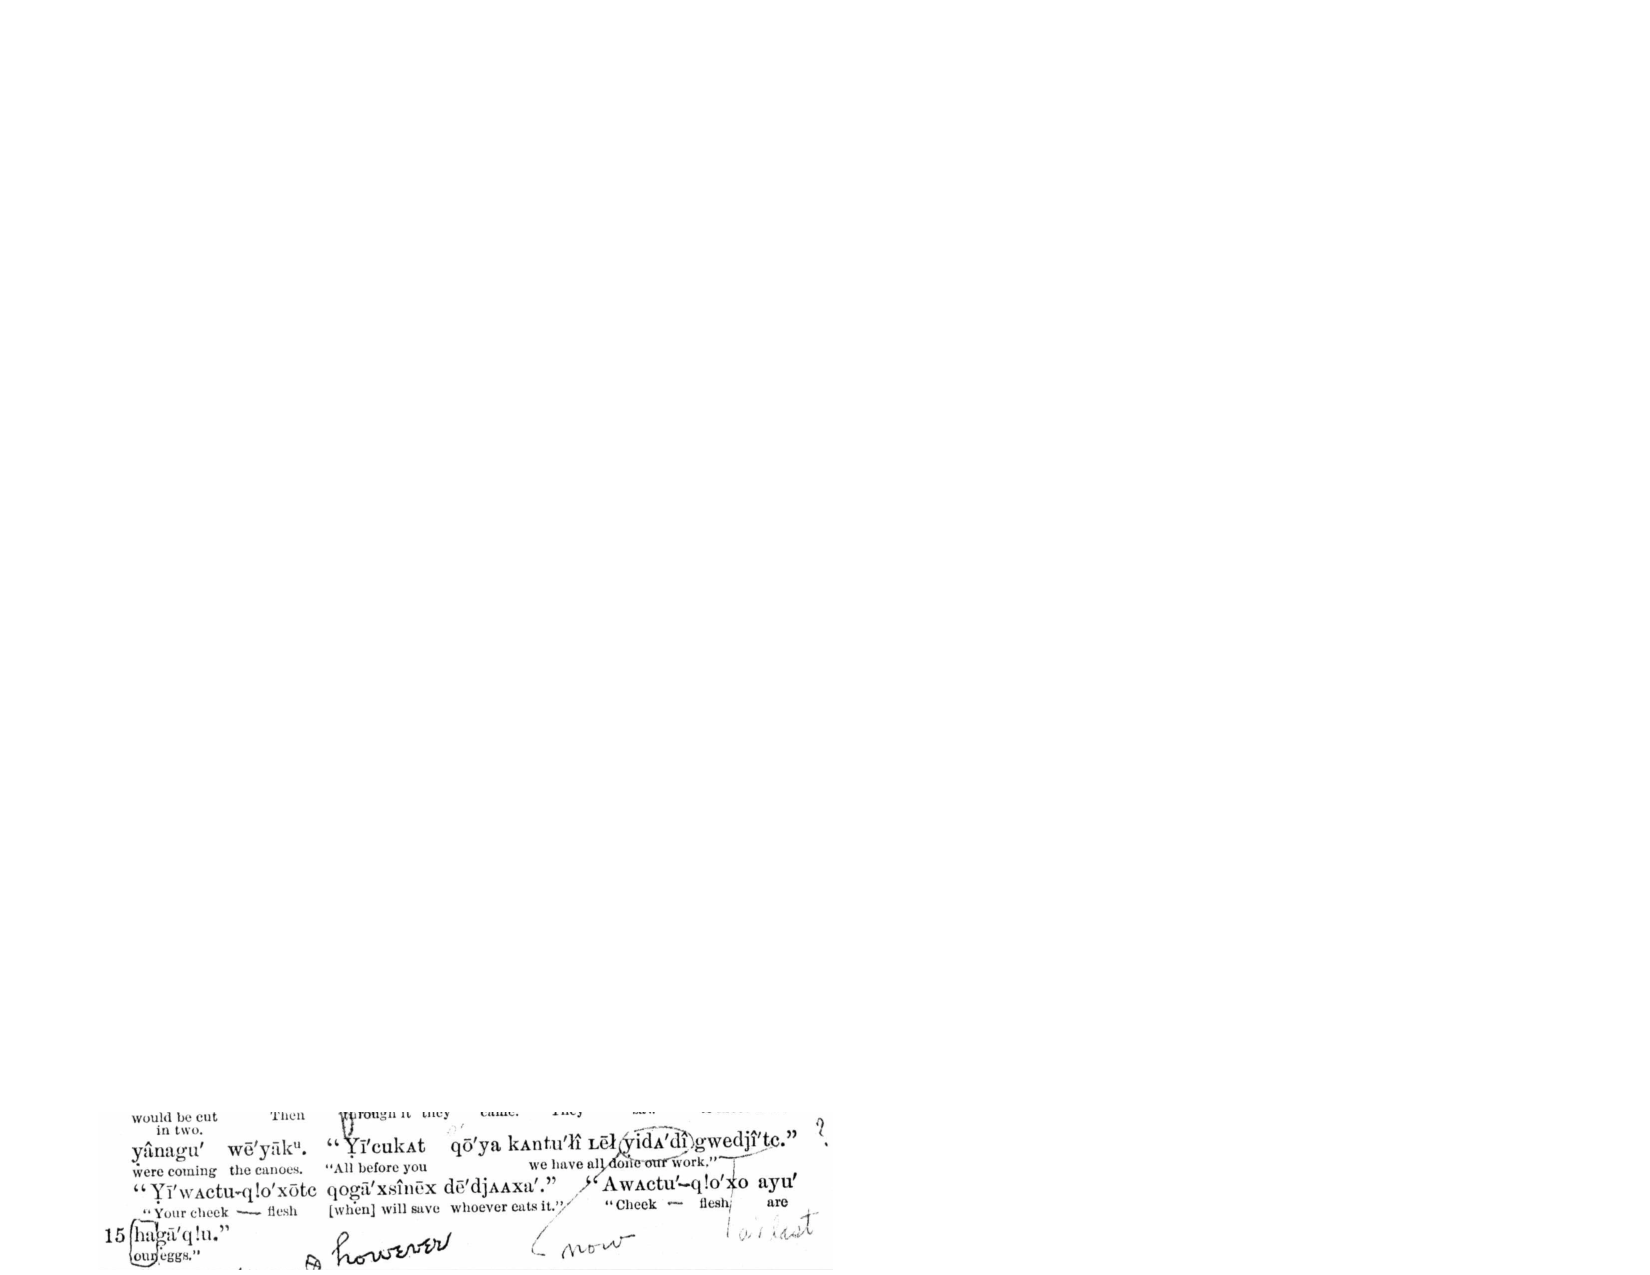
\includegraphics[width=0.9\textwidth]{figures/paul-1930-314-13.pdf}
\caption[Annotations of p.\ 314 l.\ 13 in Paul 1930]{Annotations of page 314 line 13 in \cite{paul:1930}}\label{fig:100-91-gweijich-paul-1930}
\end{figure}

\fm{Shgwínde} William L.\ Paul’s annotated copy of \cite{swanton:1909} \parencite{paul:1930} can be useful in cases like this because \citeauthor{paul:1930} occasionally offers alternative interpretations of words or phrases in \citeauthor{swanton:1909}’s transcription.
Unfortunately only a scan of a poor photocopy of this book is publicly available and consequently many of the marginalia – particularly those written in pencil – are difficult or impossible to read.
We would greatly benefit from a high resolution full colour scan of the original book with \citeauthor{paul:1930}’s notes.
For the sentence in (\lastx) \citeauthor{paul:1930} provides two annotations that can be see in figure \ref{fig:100-91-gweijich-paul-1930}.
The first is a circle around \orth{ỵidᴀ′dî} with a note below reading “now”.
This suggests that this is a form of \fm{ÿeedát} ‘moment; now’.
The second annotation is an underline below \orth{gwedjî′tc} with a faded note below it probably reading “at last”.
In addition there is a question mark in the inner margin after the end of the sentence, suggesting that the whole thing was as unclear to \citeauthor{paul:1930} as it is to us.

The first orthographic unit \orth{Ỵī′cukᴀt} in (\lastx) is clearly identifiable as \fm{ÿee shukát} ‘before you (pl.)’.
The second unit \orth{qō′ya} is probably a rendition of a common contraction of the contrastive particle \fm{ḵu.aa} ‘however, but’ and the focus particle \fm{áyá}.
It is transcribed here as the conventional form \fm{ḵu.aayá} [\ipa{qʰʷù.ˈʔàː.já}] but Ḵaadashaan’s pronunciation was probably more like a disyllabic \fm{ḵwaayá} [\ipa{ˈqʰʷà.já}] or \fm{ḵooyá} [\ipa{ˈqʰʷù.já}].

The third orthographic unit in (\lastx) is \orth{kᴀntu′łî} which is one of the two most difficult parts of this sentence.
At first blush it appears to represent something like \fm{kantóoli} [\ipa{kʰàn.ˈtʰúː.ɬì}], suggesting a verb based on the root \fm{\rt[²]{tul}} ‘spin, roll, drill’ as in \vblex{atóol}{∅}{\fm{-μμH} activity}{s/he drills it} and \vblex{aklatool}{∅/n}{\fm{-μ} activity}{s/he spins it, rolls it up} \parencites[07/11–14]{leer:1973}.
There is a phonologically similar root \fm{\rt[²]{tuʼl}} ‘murmur’ \parencites[07/16]{leer:1973} as well as a noun \fm{tóol} ‘sloping hill, plateau’ \parencites[07/17]{leer:1973}, but neither of these seems to fit here.
The interpretation of \orth{kᴀntu′łî} as \fm{kantóoli} is problematic because it appears to be an adjunct clause with no main clause verb and because it would mean e.g.\ ‘having rolled/spun (it)’ which is difficult to fit into the current discourse.

Another possible avenue is to interpret the \fm{tu-} as a first person plural subject matching \citeauthor{swanton:1909}’s translation.
This implies a form like \fm{kantoolée} suggesting a verb based on the root \fm{\rt[¹]{liʰ}} \~\ \fm{\rt[¹]{leʰ}} ‘far, distant’, which further leads to something like “it is far ahead of you”.
But  \fm{tu-} is a subject which is ungrammatical with \fm{\rt[¹]{liʰ}} ‘far, distant’ unless there is also a causative \fm{l-} prefix, meaning that the form would have to be something like \fm{kantuli̥lée} [\ipa{kʰàn.tʰùɬ.ˈɬíː}] ‘we have finally made it distant (ahead of you)’.
There must be an object in this case, but there is no obvious candidate.

Instead of the root \fm{\rt[¹]{liʰ}}, the stem in \orth{kᴀntu′łî} might instead be \fm{–léet} or \fm{–lít} and thus be based on either of the roots \fm{\rt[²]{lit}} ‘scatter, throw pl.’ or \fm{\rt[¹]{lit}} ‘slide’ \parencites[08/43–48]{leer:1973}[445–447]{leer:1976}.
The absence of \fm{t} in \citeauthor{swanton:1909}’s transcription could be explained by his mishearing it as part of the onset of the following \fm{tléil} [\ipa{tɬʰéːɬ}].
If we assume the root is \fm{\rt[²]{lit}} ‘scatter, throw pl.’ then we might suppose a form like \fm{kantuwaléet} ‘we have finally scattered them’, with \citeauthor{swanton:1909} mishearing [\ipa{ˌtʰù.wà}] as [\ipa{ˌtʰùː}].
The object of scattering might then be the \fm{gáaxʼw} ‘herring eggs’ of (\ref{ex:100-93-our-cheek-flesh}), but this seems unlikely given the intervening sentence in (\ref{ex:100-92-your-cheek-flesh}) with a different object.
If instead we assume that the root is  \fm{\rt[¹]{lit}} ‘slide’ then we could suppose a form like  \fm{kantuwaléet} ‘we have finally slid’.
This motion verb is known to be used with canoes as in the sentence \fm{Yaakw héent uwalít} ‘The canoe slid into the water’ \parencite[196.2725]{story-naish:1973}.
This interpretation is adopted in (\lastx) because it seems like the most plausible of the hypothetical readings in this narrative context.

The final word that \citeauthor{swanton:1909} transcribes as \orth{gwedjî′tc} in (\nextx) is obscure.
It appears to be \fm{gwéijích} as attested in one phrase recorded by \textcite[f05/212]{leer:1973}: “\fm{we.é tlèn gwéijích} you old thing you! (S)”, where \fm{we.é} is the second person singular independent pronoun and \fm{tlein} is ‘big, large’.
The \fm{we.é} instead of \fm{wa.é} suggests that this is from an Inland Tlingit speaker, but the “(S)” suggests a Southern speaker so the origin of this sentence is unclear.
The word \fm{gwéijích} is otherwise unknown. 

\ex\label{ex:100-92-your-cheek-flesh}%
\exmn{314.14}%
\begingl
	\glpreamble	“Ỵī′wᴀctu q!o′xōtc qog̣ā′xsînēx dē′djᴀᴀxa′.” //
	\glpreamble	Ÿee washtux̱ʼúx̱uch ḵug̱waax̱sineix̱; de chʼa ax̱á. //
	\gla	{} Ÿee \rlap{washtux̱ʼúx̱uch} @ {} @ {} @ {} @ {} {}
		\rlap{ḵug̱waax̱sineix̱;} @ {} @ {} @ {} @ {} @ {} @ {} @ {} +
		de chʼa \rlap{ax̱á.\!»} @ {} @ {} //
	\glb	{} ÿee wásh- tú- x̱ʼúx̱ -í -ch {}
		ḵu- w- g̱- g̱- s- i- \rt[¹]{nix̱} -μμL
		de chʼa a- \rt{x̱a} -H //
	\glc	{}[\pr{DP} \xx{2pl}·\xx{pss} cheek- inside- flesh -\xx{pss} -\xx{erg} {}]
		\xx{4h·o}- \xx{irr}- \xx{g̱cnj}- \xx{mod}- \xx{csv}- \xx{stv}- \rt[¹]{safe} -\xx{var}
		now just \xx{arg}- \rt[²]{eat} -\xx{var} //
	\gld	{} your cheek- inside- flesh -of {} {}
		\rlap{people.\xx{pot}.make.safe} {} {} {} {} {} {} {}
		now just \rlap{3>3.\xx{zcnj}.\xx{impfv}.eat} {} {} //
	\glft	‘Your cheek flesh can save people; they just eat it now.’
		%\exvblex{O-S-s-\rt{nex̱}}{g̱}{achievement, \fm{-tʼ} repetitive}{S make O safe, S save, rescue O}
		%\exvblex{O-S-∅-\rt{x̱a}}{∅}{\fm{-H} activity}{S eat O}
		//
\endgl
\xe

\label{note:100-fish-flesh-discussion}
The sentence in (\lastx) is the first occurrence of the word \fm{washtux̱ʼúx̱u} ‘cheek flesh’.
This is based on the relatively obscure noun \fm{x̱ʼúx̱} ‘fish flesh’ \parencite[f01/199]{leer:1973} which specifically describes the flesh of fish as distinct from \fm{dleeÿ} ‘meat, flesh’ for all other animals (birds, mammals, etc.), though today \fm{dleeÿ} is typically also used for fish.
The noun \fm{x̱ʼúx̱} ‘fish flesh’ may be related to the root \fm{\rt{x̱ʼish}} seen in \fm{atx̱ʼéeshi} ‘dryfish’ discussed earlier on page \pageref{note:100-dryfish-discussion}.
The cheek flesh of a large fish is prized as some of the highest quality meat despite being relatively small; for example, \fm{cháatl washtux̱ʼúx̱u} ‘halibut cheeks’ are often given as gifts to elders.

\ex\label{ex:100-93-our-cheek-flesh}%
\exmn{314.14}%
\begingl
	\glpreamble	“Awᴀctu′ q!o′xo ayu′ hag̣ā′q!u.” //
	\glpreamble	Haa washtux̱ʼúx̱u áyú haa g̱áaxʼu.\!» //
	\gla	{} Haa \rlap{washtux̱ʼúx̱u} @ {} @ {} @ {} {}
		\rlap{áyú} @ {}
		{} haa \rlap{g̱áaxʼu.\!»} @ {} {} //
	\glb	{} haa wásh- tú- x̱ʼúx̱ -í {}
		á -yú
		{} haa g̱áaxʼw -í {} //
	\glc	{}[\pr{DP} \xx{1pl}·\xx{pss} cheek- inside- flesh -\xx{pss} {}]
		\xx{cpl} -\xx{dist}
		{}[\pr{DP} \xx{1pl}·\xx{pss} herring·egg -\xx{pss} {}] //
	\gld	{} our cheek- inside- flesh -of {}
		\rlap{it.is} {}
		{} our \rlap{herring·eggs} {} {} //
	\glft	‘Our herring eggs are our cheek flesh.”’
		//
\endgl
\xe

\section{Paragraph 7}\label{sec:100-para-7}

\ex\label{ex:100-94-came-to-each-other}%
\exmn{315.1}%
\begingl
	\glpreamble	Adᴀ′xayu wucxᴀ′nt hᴀs ỵa′odîgu yū′xāt. //
	\glpreamble	Aadáx̱ áyú woosh x̱ánt has ÿawdigóo yú x̱áat. //
	\gla	{} \rlap{Aadáx̱} @ {} {} \rlap{áyú} @ {} 
		{} woosh \rlap{x̱ánt} @ {} {}
		has @ \rlap{ÿawdigóo} @ {} @ {} @ {} @ {} @ {} +
		{} yú x̱áat. {} //
	\glb	{} á -dáx̱ {} á -yú 
		{} woosh x̱án -t {}
		has= ÿ- wu- d- i- \rt{gu} -μμH
		{} yú x̱áat {} //
	\glc	{}[\pr{PP} \xx{3n} -\xx{abl} {}] \xx{foc} -\xx{dist}
		{}[\pr{PP} \xx{recip}·\xx{pss} near -\xx{pnct} {}]
		\xx{plh}= \xx{qual}- \xx{pfv}- \xx{mid}- \xx{stv}- \rt[¹]{poke} -\xx{var}
		{}[\pr{DP} \xx{dist} salmon {}] //
	\gld	{} that -after {} \rlap{it.is} {}
		{} ea·other’s near -to {}
		they \rlap{\xx{zcnj}.\xx{pfv}.swim·group} {} {} {} {} {}
		{} those salmon {} //
	\glft	‘After that they came near to each other, those salmon.’
		%\exvblex{ÿ-S-∅-\rt{gu}}{}{motion}{S (pl.\ group) swim}
		%+ \exvblex*{NP-\{t,x̱,dé\}}{∅}{\fm{-μ} repetitive}{arriving at NP}
		//
\endgl
\xe

\ex\label{ex:100-95-they-say}%
\exmn{315.1}%
\begingl
	\glpreamble	Ye hᴀs q!ā′ỵaqa, //
	\glpreamble	Yéi has x̱ʼaÿaḵá //
	\gla	Yéi @ has @ \rlap{x̱ʼaÿaḵá} @ {} @ {} @ {} //
	\glb	yéi= has= x̱ʼa- ÿ- \rt{ḵa} -μH //
	\glc	thus= \xx{plh}= mouth- \xx{qual}- \rt{say} -\xx{var} //
	\gld	thus they \rlap{\xx{ncnj}.\xx{impfv}.say} {} {} {} //
	\glft	‘They say’
		%\exvblex{yéi=(x̱ʼe)-ÿ-S-∅-\rt{ḵa}}{n}{\fm{x̱ʼe-…-H} activity}{S say thus}
		//
\endgl
\xe

\ex\label{ex:100-96-they-say}%
\exmn{315.2}%
\begingl
	\glpreamble	“Gudē′sa ỵī′ỵᴀkᵘgwaha.” //
	\glpreamble	«\!Goodé sá ÿee ÿakwg̱waháa?\!». //
	\gla	{} {} \llap{«\!}\rlap{Goodé} @ {} {} sá {}
		ÿee @ \rlap{ÿakwg̱waháa?\!»} @ {} @ {} @ {} @ {} @ {} //
	\glb	{} {} goo -dé {} sá {}
		ÿee= ÿ- w- g- g̱- \rt[¹]{ha} -μμH //
	\glc	{}[\pr{QP} {}[\pr{PP} where -\xx{all} {}] \xx{q} {}]
		\xx{2pl·o}= \xx{qual}- \xx{irr}- \xx{gcnj}- \xx{mod}- \rt[¹]{mv·invis} -\xx{var} //
	\gld	{} {} where -to {} ? {}
		you \rlap{\xx{zcnj}.\xx{prsp}.appear} {} {} {} {} {} //
	\glft	‘“Where are you going to appear at?”.’
		%\exvblex{O-ÿ-∅-\rt{haʰ}}{∅}{motion}{O appear}
		%+ \exvblex*{NP-\{t,x̱,dé\}}{∅}{\fm{-μ} repetitive}{arrive at NP}
		//
\endgl
\xe

\ex\label{ex:100-97-said-stikine}%
\exmn{315.2}%
\begingl
	\glpreamble	ᴀxō′a ye ỵawaqa′ “Ohā′n qō′a Stîq!hī′nde,” //
	\glpreamble	A x̱oo.aa yéi ÿaawaḵaa «\!Uháan ḵu.aa Shtaxʼhéende\!», //
	\gla	{} A \rlap{x̱oo.aa} @ {} {}
		yéi @ \rlap{ÿaawaḵaa} @ {} @ {} @ {} @ {}
		«\!Uháan ḵu.aa +
		{} \rlap{Shtaxʼhéende\!»} @ {} @ {} @ {} @ {} {} //
	\glb	{} a x̱oo- aa {} 
		yéi= ÿ- wu- i- \rt[¹]{ḵa} -μμH
		\pqp{}uháan ḵu.aa 
		{} sh- d- \rt[²]{taxʼ}- héen -dé {} //
	\glc	{}[\pr{DP} \xx{3n}·\xx{pss} among -\xx{part} {}]
		thus= \xx{qual}- \xx{pfv}- \xx{stv}- \rt[¹]{say} -\xx{var}
		\pqp{}\xx{1pl} \xx{contr}
		{}[\pr{PP} \xx{rflx}- \xx{mid}- \rt[²]{bite}- river -\xx{all} {}] //
	\gld	{} them among -some {}
		thus= \rlap{\xx{ncnj}.\xx{pfv}.say} {} {} {} {}
		\pqp{}us however
		{} \rlap{Stikine} {} {} {} -to {} //
	\glft	‘Some among them said “Us however, we are to the Stikine”,’
		%\exvblex{yéi=(x̱ʼe)-ÿ-S-∅-\rt{ḵa}}{n}{\fm{x̱ʼe-…-H} activity}{S say thus}
		//
\endgl
\xe

From (\ref{ex:100-97-said-stikine}) to (\ref{ex:100-101-alsek}) the salmon people speak in sentences that consist solely of a PP headed by the allative postposition \fm{-dé} ‘to, toward’.
The initial sentence in (\lastx) has a quotative speech verb from the narrator, but for the rest of the sentences this verb is implicit.
One additional speech verb is added in (\ref{ex:100-99-taku}) for ease of reading.

\ex\label{ex:100-98-chilkat}%
\exmn{315.3}%
\begingl
	\glpreamble	axō′a “Qō′a Djîłqā′tdê,” //
	\glpreamble	a x̱oo.aa ḵu.aa «\!Jilḵáatde\!», //
	\gla	{} a \rlap{x̱oo.aa} @ {} {} ḵu.aa 
		{} \llap{«\!}\rlap{Jilḵáatde\!»,} @ {} {} //
	\glb	{} a x̱oo- aa {} ḵu.aa
		{} Jilḵáat -dé {} //
	\glc	{}[\pr{DP} \xx{3n}·\xx{pss} among -\xx{part} {}] \xx{contr} 
		{}[\pr{PP} \xx{name} -\xx{all} {}] //
	\gld	{} them among -some {} however 
		{} Chilkat -to {} //
	\glft	‘some however said “to the Chilkat”,’
		//
\endgl
\xe

\ex\label{ex:100-99-taku}%
\exmn{315.3}%
\begingl
	\glpreamble	axō′a “T!aqo′dê,” //
	\glpreamble	a x̱oo.aa «\!Tʼaaḵóode\!», //
	\gla	{} a \rlap{x̱oo.aa} @ {} {} 
		{} \llap{«\!}\rlap{Tʼaaḵóode\!»,} @ {} {} //
	\glb	{} a x̱oo- aa {}
		{} Tʼaaḵú -dé {} //
	\glc	{}[\pr{DP} \xx{3n}·\xx{pss} among -\xx{part} {}]
		{}[\pr{PP} \xx{name} -\xx{all} {}] //
	\gld	{} them among -some {} 
		{} Taku -to {} //
	\glft	‘some “to the Taku”,’
		//
\endgl
\xe

\ex\label{ex:100-100-nass}%
\exmn{315.3}%
\begingl
	\glpreamble	axō′a “Nā′sdê,” //
	\glpreamble	a x̱oo.aa «\!Naasdé\!», //
	\gla	{} a \rlap{x̱oo.aa} @ {} {} 
		{} \llap{«\!}\rlap{Naasdé\!»,} @ {} {} //
	\glb	{} a x̱oo- aa {}
		{} Naas -dé {} //
	\glc	{}[\pr{DP} \xx{3n}·\xx{pss} among -\xx{part} {}]
		{}[\pr{PP} \xx{name} -\xx{all} {}] //
	\gld	{} them among -some {} 
		{} Nass -to {} //
	\glft	‘some “to the Nass”,’
		//
\endgl
\xe

\ex\label{ex:100-101-alsek}%
\exmn{315.4}%
\begingl
	\glpreamble	axō′a “Ałsē′xdê.” //
	\glpreamble	a x̱oo.aa «\!Aalséix̱de\!». //
	\gla	{} a \rlap{x̱oo.aa} @ {} {} 
		{} \llap{«\!}\rlap{Aalséix̱de\!».} @ {} {} //
	\glb	{} a x̱oo- aa {}
		{} Aalséix̱ -dé {} //
	\glc	{}[\pr{DP} \xx{3n}·\xx{pss} among -\xx{part} {}]
		{}[\pr{PP} \xx{name} -\xx{all} {}] //
	\gld	{} them among -some {} 
		{} Alsek -to {} //
	\glft	‘some said “to the Alsek”.’
		//
\endgl
\xe

\ex\label{ex:100-102-name-all-rivers}%
\exmn{315.4}%
\begingl
	\glpreamble	Djîłdakᴀ′t yahī′n hᴀs awasā′kᵘ. //
	\glpreamble	Chʼa ldakát yá héen has aawasáakw. //
	\gla	{} Chʼa ldakát yá héen {} 
		has @ \rlap{aawasáakw.} @ {} @ {} @ {} @ {} @ {} //
	\glb	{} chʼa ldakát yá héen {}
		has= a- wu- i- \rt[²]{sa} -μμH -kw //
	\glc	{}[\pr{DP} just all \xx{prox} river {}]
		\xx{plh}= \xx{arg}- \xx{pfv}- \xx{stv}- \rt[²]{name} -\xx{var} -\xx{rep} //
	\gld	{} just all these rivers {}
		they \rlap{3>3.\xx{zcnj}.\xx{pfv}.name.\xx{rep}} {} {} {} {} {} //
	\glft	‘They named all of the rivers.’
		%\exvblex{O-S-∅-\rt{sa}-μH-kw}{∅}{\fm{-μH-kw} repetitive state}{S call, name O}
		//
\endgl
\xe

\ex\label{ex:100-103-name-all-rivers}%
\exmn{315.5}%
\begingl
	\glpreamble	Adᴀ′xawe hīn wᴀtt wus!îx̣ī′x̣ wē′xāt. //
	\glpreamble	Aadáx̱ áwé héen wátt wusixeex wé x̱áat. //
	\gla	{} \rlap{Aadáx̱} @ {} {} \rlap{áwé} @ {} 
		{} héen \rlap{wátt} @ {} {}
		\rlap{wusixeex} @ {} @ {} @ {} @ {}
		{} wé x̱áat. {} //
	\glb	{} á -dáx̱ {} á -wé
		{} héen wát -t {} 
		wu- s- i- \rt[¹]{xix} -μμL
		{} wé x̱áat {} //
	\glc	{}[\pr{PP} \xx{3n} -\xx{abl} {}] \xx{foc} -\xx{mdst}
		{}[\pr{PP} river mouth -\xx{pnct} {}]
		\xx{pfv}- \xx{xtn}- \xx{stv}- \rt[¹]{fall} -\xx{var}
		{}[\pr{DP} \xx{mdst} salmon {}] //
	\gld	{} then -after {} \rlap{it.is} {} 
		{} river mouth -around {}
		\rlap{\xx{ncnj}.\xx{pfv}.disperse} {} {} {} {}
		{} those salmon {} //
	\glft	‘Then they spread out around the river mouths, those salmon.’
		%\exvblex{NP-t O-s-\rt{xix}}{n}{motion, \fm{yoo=i-…-k} repetitive}{O disperse, fall out around NP}
		//
\endgl
\xe

\ex\label{ex:100-104-someone-said}%
\exmn{315.5}%
\begingl
	\glpreamble	Ye qoỵā′waqa //
	\glpreamble	Yéi ḵuÿaawaḵaa //
	\gla	Yéi @ \rlap{ḵuÿaawaḵaa} @ {} @ {} @ {} @ {} @ {} //
	\glb	yéi= ḵu- ÿ- wu- i- \rt[¹]{ḵa} -μμL //
	\glc	thus= \xx{4h·s}- \xx{qual}- \xx{pfv}- \xx{stv}- \rt[¹]{say} -\xx{var} //
	\gld	thus \rlap{one.\xx{ncnj}.\xx{pfv}.say} {} {} {} {} {} //
	\glft	‘Someone said’
		%\exvblex{yéi=(x̱ʼe)-ÿ-S-∅-\rt{ḵa}}{n}{\fm{x̱ʼe-…-H} activity}{S say thus}
		//
\endgl
\xe

The verb \vblex{yéi x̱ʼayaḵá}{n}{\fm{x̱ʼe-…-μH} activity}{s/he says thus} used in (\lastx) has unique behaviour when it is used with the fourth person human subject ‘someone, they, people’.
Normally this subject is the prefix \fm{du-}, but for this verb the same fourth person human subject is represented by the fourth person human object prefix \fm{ḵu-}.
Thus instead of the expected \fm[*]{yéi yawduwaḵaa} ‘someone said, people said’ the form is \fm{yéi ḵuyaawaḵaa} as (\lastx).
This irregularity is shared by other languages in the Na-Dene family such as Koyukon \fm{dehʉdegheeneeʼ} ‘people said so’ with the \fm{hʉ-} that is cognate to Tlingit \fm{ḵu-} \parencite[437]{jette-jones:2000}.

\ex\label{ex:100-105-someone-said}%
\exmn{315.5}%
\begingl
	\glpreamble	“Yākᵘ nᴀx ā′gūx dᴀhā′nî.” //
	\glpreamble	«\!Yaakwnáx̱ áa gux̱daháani.\!» //
	\gla	{} \llap{«\!}\rlap{Yaakwnáx̱} @ {} {}
		{} \rlap{áa} @ {} {}
		\rlap{gux̱daháani.\!»} @ {} @ {} @ {} @ {} @ {} @ {} //
	\glb	{} yaakw -náx̱ {} 
		{} á -μ {}
		w- g- g̱- d- \rt[¹]{han} -μμH -í //
	\glc	{}[\pr{PP} boat -\xx{perl} {}]
		{}[\pr{PP} \xx{3n} -\xx{loc} {}]
		\xx{irr}- \xx{gcnj}- \xx{mod}- \xx{mid}- \rt[¹]{stand·\xx{sg}} -\xx{var} -\xx{sub} //
	\gld	{} boat -along {}
		{} there -at {}
		\rlap{\xx{ncnj}.\xx{prsp}.stand·\xx{sg}} {} {} {} {} {} {} -\xx{sub} //
	\glft	‘“He will stand up there alongside the boat”.’
		%\exvblex{S-d-∅-\rt{han}}{g}{achievement}{S (sg.)\ stand up}
		%+ \exvblex*{NP-xʼ}{∅}{\fm{-x̱} repetitive}{near NP}
		%\newline+ \exvblex*{NP-náx̱}{n}{\fm{yoo=i-…-k} repetitive}{via, through, across, along NP}
		//
\endgl
\xe

\ex\label{ex:100-106-jumper-stood-up}%
\exmn{315.6}%
\begingl
	\glpreamble	Adᴀ′xayu qᴀdu′ ke wutā′nî ᴀsgē′yu yākᵘ nᴀx wudîhā′n. //
	\glpreamble	Aadáx̱ áyú ḵáju kei wutáani ásgéyú yaakwnáx̱ wudihaan. //
	\gla	{} \rlap{Aadáx̱} @ {} {} \rlap{áyú} @ {} 
		ḵáju
		{} kei @ \rlap{wutáani} @ {} @ {} @ {} {}
		\rlap{ásgéyú} @ {} @ {} @ {} +
		{} \rlap{yaakwnáx̱} @ {} {}
		\rlap{wudihaan} @ {} @ {} @ {} @ {} //
	\glb	{} á -dáx̱ {} á -yú
		ḵáju
		{} kei= wu- \rt[¹]{taʼn} -μμH -í {}
		á -sí -gí -yú
		{} yaakw -náx̱ {}
		wu- d- i- \rt[¹]{han} -μμL //
	\glc	{}[\pr{PP} \xx{3n} -\xx{abl} {}] \xx{foc} -\xx{dist} 
		actually
		{}[\pr{DP} up= \xx{pfv}- \rt[¹]{fish·jump} -\xx{var} -\xx{nmz} {}]
		\xx{foc} -\xx{dub} -\xx{yn} -\xx{dist}
		{}[\pr{PP} boat -\xx{perl} {}]
		\xx{pfv}- \xx{mid}- \xx{stv}- \rt[¹]{stand·\xx{sg}} -\xx{var} //
	\gld	{} that -after {} \rlap{it.is} {}
		actually
		{} up \rlap{jumping·fish} {} {} {} {}
		it.is \·\rlap{maybe} {} {}
		{} boat -along {}
		\rlap{\xx{ncnj}.\xx{pfv}.stand·\xx{sg}} {} {} {} {} //
	\glft	‘Then actually it’s a jumper who apparently stood up alongside the boat.’
		%\exvblex{S-∅-\rt{taʼn}}{}{motion}{S (fish) jump out of water}
		%+ \exvblex*{kei=}{∅}{\fm{-ch} repetitive}{upward}
		%\exvblex{S-d-∅-\rt{han}}{g}{achievement}{S (sg.)\ stand up}
		%\newline+ \exvblex*{NP-náx̱}{n}{\fm{yoo=i-…-k} repetitive}{via, through, across, along NP}
		//
\endgl
\xe

\ex\label{ex:100-107-salmon-saying}%
\exmn{315.7}%
\begingl
	\glpreamble	Adᴀ′xayu yū′xāt ye hᴀs ỵânaqē′tc, //
	\glpreamble	Aadáx̱ áyú yú x̱áat yéi has ÿanaḵéich //
	\gla	{} \rlap{Aadáx̱} @ {} {} \rlap{áyú} @ {}
		{} yú x̱áat {}
		yéi @ has @ \rlap{ÿanaḵéich} @ {} @ {} @ {} @ {} //
	\glb	{} á -dáx̱ {} á -yú
		{} yú x̱áat {}
		yéi= has= ÿ- n- \rt[¹]{ḵa} -eμH -ch //
	\glc	{}[\pr{PP} \xx{3n} -\xx{abl} {}] \xx{foc} -\xx{dist} 
		{}[\pr{DP} \xx{dist} salmon {}]
		thus= \xx{plh}= \xx{qual}- \xx{ncnj}- \rt[¹]{say} -\xx{var} -\xx{rep} //
	\gld	{} that -after {} \rlap{it.is} {} 
		{} those salmon {}
		thus they \rlap{\xx{hab}.say} {} {} {} {} //
	\glft	‘After that those salmon were repeatedly saying’
		%\exvblex{yéi=(x̱ʼe)-ÿ-S-∅-\rt{ḵa}}{n}{\fm{x̱ʼe-…-H} activity}{S say thus}
		//
\endgl
\xe

The verbs in (\ref{ex:100-107-salmon-saying}) through (\ref{ex:100-112-he-said}) are all marked for habitual aspect.
The habitual is used here because it introduces a meaning of repetition so that this sequence describes a series of events where the salmon people ask about the fort, send someone to check, and that one returns to report.
The forms in (\ref{ex:100-107-salmon-saying}), (\ref{ex:100-109-told-one-go-in-sight}), and (\ref{ex:100-112-he-said}) show the characteristic combination of the \fm{n-} conjugation prefix and the \fm{-ch} repetitive suffix that together regularly form the habitual aspect for \fm{n}-conjugation verbs.
The forms in (\ref{ex:100-108-fort-ready}) and (\ref{ex:100-111-swam-back}) have the \fm{∅}-conjugation perfective prefix \fm{u-} along with repetitive \fm{-ch} that together indicate the habitual aspect for \fm{∅}-conjugation verbs.
In (\ref{ex:100-108-fort-ready}) the \fm{u-} is lengthened by the irrealis \fm{u-} that appears because the verb is negated and in (\ref{ex:100-111-swam-back}) the \fm{u-} is preceded by the qualifier \fm{ÿ-} which together form a syllable \fm{wu} [\ipa{wù}].

\clearpage
\ex\label{ex:100-108-fort-ready}%
\exmn{315.7}%
\begingl
	\glpreamble	“Yū′nū ᴀgî′ ʟēł yên unī′tc.” //
	\glpreamble	«\!Yú noow ágí tléil yan ooneech?\!». //
	\gla	{} \llap{«\!}Yú noow {} \rlap{ágí} @ {}
		tléil yan @ \rlap{ooneech?\!».} @ {} @ {} @ {} @ {} //
	\glb	{} yú noow {} á -gí 
		tléil ÿán= u- u- \rt[¹]{niʰ} -μμL -ch //
	\glc	{}[\pr{DP} \xx{dist} fort {}] \xx{foc} -\xx{yn} 
		\xx{neg} \xx{term}= \xx{irr}- \xx{zpfv}- \rt[¹]{happen} -\xx{var} -\xx{rep} //
	\gld	{} that fort {} is.it \·?
		not done \rlap{\xx{hab}.happen} {} {} {} {} //
	\glft	‘“Isn’t that fort ready?”.’
		%\exvblex{yéi=O-∅-\rt{niʰ}}{n}{achievement, \fm{-μ-n} progressive}{O happen; happen thus to O}
		//
\endgl
\xe

\ex\label{ex:100-109-told-one-go-in-sight}%
\exmn{315.8}%
\begingl
	\glpreamble	Tc!uʟe′ ʟē′nᴀx ᴀkīkᴀ′ndî akᴀ′nduqē′tc. //
	\glpreamble	Chʼu tle tléináx̱ a keekánde aa kanduḵéich. //
	\gla	Chʼu tle {} \rlap{tléináx̱} @ {} {} 
		{} a \rlap{keekánde} @ {} {}
		aa @ \rlap{kanduḵéich} @ {} @ {} @ {} @ {} @ {} //
	\glb	chʼu tle {} tléixʼ -náx̱ {} 
		{} a keekán -dé {}
		aa= k- n- du- \rt[¹]{ḵa} -eμH -ch //
	\glc	just then {}[\pr{DP} one -\xx{hum} {}]
		{}[\pr{PP} \xx{3n}·\xx{pss} vision -\xx{all} {}]
		\xx{part·o}= \xx{qual}- \xx{ncnj}- \xx{4h·s}- \rt[¹]{say} -\xx{var} -\xx{rep} //
	\gld	just then {} \rlap{one.person} {} {} 
		{} its vision -to {}
		some \rlap{\xx{hab}.people.order} {} {} {} {} {} //
	\glft	‘So then they repeatedly told one of them to go into the sight of it.’
		%\exvblex{yéi=O-k-(u)-S-∅-\rt{ḵa}}{n}{\fm{-H} activity}{S tell O to do thus}
		//
\endgl
\xe

\ex\label{ex:100-110-apparently-fish-trap}%
\exmn{315.8}%
\begingl
	\glpreamble	Hᴀdju′ yucā′ł ᴀ′sgîyu yunū′wu ye hᴀs aỵasā′kᵘ. //
	\glpreamble	X̱áju yú sháal ásgíyú yú noow yéi has aÿasáakw. //
	\gla	X̱áju 
		{} yú sháal {} \rlap{ásgíyú} @ {} @ {} @ {} 
		{} yú noow {}
		yéi @ has @ \rlap{aÿasáakw.} @ {} @ {} @ {} //
	\glb	x̱áju 
		{} yú sháal {} á -s -gí -yú 
		{} yú noow {}
		yéi= has= a- i- \rt[¹]{sa} -μμH -kw //
	\glc	actually 	
		{}[\pr{DP} \xx{dist} fishtrap {}] \xx{foc} -\xx{dub} -\xx{yn} -\xx{dist}
		{}[\pr{DP} \xx{dist} fort {}]
		thus= \xx{plh}= \xx{arg}- \xx{stv}- \rt[¹]{name} -\xx{var} -\xx{rep} //
	\gld	actually
		{} that fishtrap {} it.is \·\rlap{maybe} {} {}
		{} that fort {}
		thus they \rlap{3>3.\xx{zcnj}.\xx{impfv}.call.\xx{rep}} {} {} {} //
	\glft	‘Actually it’s apparently a fish trap that they keep calling a fort.’
		%\exvblex{O-S-∅-\rt{sa}-μH-kw}{∅}{\fm{-μH-kw} repetitive state}{S call, name O}
		//
\endgl
\xe

\ex\label{ex:100-111-swam-back}%
\exmn{315.9}%
\begingl
	\glpreamble	Tc!uʟe′ qox wudaq!ā′ktc ye ỵânaqē′tc //
	\glpreamble	Chʼu tle ḵux̱ wudaxʼaakch. //
	\gla	Chʼu tle ḵux̱ @ \rlap{wudaxʼaakch.} @ {} @ {} @ {} @ {} @ {} //
	\glb	chʼu tle ḵúx̱= ÿ- u- d- \rt[¹]{x̱ʼak} -μμL -ch //
	\glc	just then \xx{rev}= \xx{qual}- \xx{zpfv}- \xx{mid}- \rt[¹]{swim} -\xx{var} -\xx{rep} //
	\gld	just then back \rlap{\xx{hab}.swim} {} {} {} {} {} //
	\glft	‘So then he always swims back.’
		%\exvblex{S-d-∅-\rt{xʼak}}{}{motion}{S (fish) swim}
		%+ \exvblex*{ḵúx̱(-dé) d-}{∅}{\fm{-ch} repetitive}{reverting, returning directly}
		%\exvblex{yéi=(x̱ʼe)-ÿ-S-∅-\rt{ḵa}}{n}{\fm{x̱ʼe-…-H} activity}{S say thus}
		//
\endgl
\xe

%The verb that Swanton transcribes as \fm{qox wudaq!ā′ktc} in (\nextx) is particularly interesting.
Swanton’s gloss is “back every time he came”, presumably reflecting Ḵadishaan’s intention and suggesting that the verb root is actually \fm{\rt{xʼak}} ‘(fish) swim’.
This root may be related to two other roots \fm{\rt{x̱ʼakw}} ‘(salmon) turn red’ and \fm{\rt{xʼaḵw}} ‘come to end, die’.
The \fm{qox} of Swanton’s transcription is certainly the revertive motion derivation with \fm{ḵúx̱(-dé)} which is accompanied by middle voice \fm{d-} in the classifier because \fm{ḵúx̱} entails the start and end of a path being identical, similar to the agent and patient of a reflexive being identical.
The initial \fm{wu} in Swanton’s transcription could be taken to represent the \fm{wu-} perfective prefix, but because the revertive motion derivation is \fm{∅}-conjugation we instead expect the \fm{∅}-conjugation perfective \fm{u-} \xx{zpfv}.
I interpret the \fm{wu-} as indicating the presence of a preceding \fm{ÿ-} qualifier, though I am uncertain what this contributes.
The \fm{ÿ-} is found in some motion derivations that describe paths oblique to the origo, as well as the perambulative revertive derivation \vblex{a-ÿ-d-}{∅}{\fm{-x̱} repetitive}{turning back} that describes a path which returns indirectly or circuitously to the start.

\ex\label{ex:100-112-he-said}%
\exmn{315.10}%
\begingl
	\glpreamble	ye ỵânaqē′tc //
	\glpreamble	Yéi ÿanaḵéich //
	\gla	Yéi @ \rlap{ÿanaḵéich} @ {} @ {} @ {} @ {} //
	\glb	yéi= ÿ- n- \rt[¹]{ḵa} -eμH -ch //
	\glc	thus= \xx{qual}- \xx{ncnj}- \rt[¹]{say} -\xx{var} -\xx{rep} //
	\gld	thus \rlap{\xx{hab}.say} {} {} {} {} //
	\glft	‘He keeps saying’
		%\exvblex{S-d-∅-\rt{xʼak}}{}{motion}{S (fish) swim}
		%+ \exvblex*{ḵúx̱(-dé) d-}{∅}{\fm{-ch} repetitive}{reverting, returning directly}
		%\exvblex{yéi=(x̱ʼe)-ÿ-S-∅-\rt{ḵa}}{n}{\fm{x̱ʼe-…-H} activity}{S say thus}
		//
\endgl
\xe

\ex\label{ex:100-113-getting-toward-done}%
\exmn{315.10}%
\begingl
	\glpreamble	“Deyêndê ỵanᴀnī′n.” //
	\glpreamble	«\!De yánde ÿaa naneen\!». //
	\gla	«\!De 
		{} \rlap{yánde} @ {} {} 
		ÿaa @ \rlap{naneen\!».} @ {} @ {} @ {} @ {} @ {} @ {} //
	\glb	\pqp{}de
		{} ÿán -dé {} 
		ÿaa= n- \rt[¹]{niʰ} -μμL -n //
	\glc	\pqp{}now
		{}[\pr{PP} \xx{term} -\xx{all} {}]
		along= \xx{ncnj}- \rt[¹]{happen} -\xx{var} -\xx{nsfx} //
	\gld	\pqp{}now
		{} done -toward {}
		along \rlap{\xx{zcnj}.\xx{prog}.happen} {} {} {} {} {} {} //
	\glft	‘“It’s still becoming ready”.’
		%\exvblex{yéi=O-∅-\rt{niʰ}}{n}{achievement, \fm{-μ-n} progressive}{O happen; happen thus to O}
		%\newline+ \exvblex*{ÿan \~\ ÿax̱ \~\ ÿánde}{∅}{\fm{-μ} repetitive}{to rest, ashore, completing}
		//
\endgl
\xe

\ex\label{ex:100-114-at-some-point-ready}%
\exmn{315.10}%
\begingl
	\glpreamble	Wananī′sayu yên uwanī′ ye ỵawaqa′. //
	\glpreamble	Wáa nanée sáyú yan uwanée yéi ÿaawaḵaa. //
	\gla	{} Wáa \rlap{nanée} @ {} @ {} @ {} {} \rlap{sáyú} @ {} @ {}
		{} yan @ \rlap{uwanée} @ {} @ {} @ {} @ {} {} 
		yéi @ \rlap{ÿaawaḵaa.} @ {} @ {} @ {} @ {}//
	\glb	{} wáa n- \rt[¹]{niʰ} -μμH {} {} s- á -yú
		{} ÿán= u- i- \rt[¹]{niʰ} -μμH {} {}
		yéi= ÿ- wu- i- \rt[¹]{ḵa} -μμL //
	\glc	{}[\pr{CP} how \xx{ncnj}- \rt[¹]{happen} -\xx{var} \·\xx{sub} {}] \xx{q}- \xx{foc} -\xx{dist}
		{}[\pr{CP} \xx{term}= \xx{zpfv}- \xx{stv}- \rt[¹]{happen} -\xx{var} \·\xx{sub} {}]
		thus= \xx{qual}- \xx{pfv}- \xx{stv}- \rt[¹]{say} -\xx{var} //
	\gld	{} how \rlap{\xx{csec}.happen} {} {} \·when {} {} \rlap{it.is} {}
		{} done \rlap{\xx{zcnj}.\xx{pfv}.happen} {} {} {} \·that {}
		thus \rlap{\xx{ncnj}.\xx{pfv}.say} {} {} {} {} //
	\glft	‘At some point he said that it had become ready.’
		%\exvblex{yéi=O-∅-\rt{niʰ}}{n}{achievement, \fm{-μ-n} progressive}{O happen; happen thus to O}
		%\newline+ \exvblex*{ÿan \~\ ÿax̱ \~\ ÿánde}{∅}{\fm{-μ} repetitive}{to rest, ashore, completing}
		%\exvblex{yéi=(x̱ʼe)-ÿ-S-∅-\rt{ḵa}}{n}{\fm{x̱ʼe-…-H} activity}{S say thus}
		//
\endgl
\xe

\ex\label{ex:100-115-fish-people-ready}%
\exmn{315.11}%
\begingl
	\glpreamble	Xāt qoa′nî de yên uwanī′. //
	\glpreamble	X̱áat ḵwáani de yan uwanée. //
	\gla	{} X̱áat \rlap{ḵwáani} @ {} {} de 
		yan @ \rlap{uwanée.}  @ {} @ {} @ {} //
	\glb	{} x̱áat ḵwáan -í {} de 
		ÿán= u- i- \rt[¹]{niʰ} -μμH //
	\glc	{}[\pr{DP} salmon people -\xx{pss} {}] now 
		\xx{term}= \xx{zpfv}- \xx{stv}- \rt[¹]{happen} -\xx{var} //
	\gld	{} salmon people –of {} now
		done \rlap{\xx{zcnj}.\xx{pfv}.happen} {} {} {} //
	\glft	‘The salmon people now got ready.’
		%\exvblex{yéi=O-∅-\rt{niʰ}}{n}{achievement, \fm{-μ-n} progressive}{O happen; happen thus to O}
		%\newline+ \exvblex*{ÿan \~\ ÿax̱ \~\ ÿánde}{∅}{\fm{-μ} repetitive}{to rest, ashore, completing}
		//
\endgl
\xe

\ex\label{ex:100-116-fish-people-ready}%
\exmn{315.11}%
\begingl
	\glpreamble	Tc!uʟe′ hīn uwaq!ᴀ′q yū′xāt. //
	\glpreamble	Chʼu tle héent uwaxʼák yú x̱áat. //
	\gla	Chʼu tle {} \rlap{héent} @ {} {} 
		\rlap{uwaxʼák} @ {} @ {} @ {} 
		{} yú x̱áat. {} //
	\glb	chʼu tle {} héen -t {} 
		u- i- \rt[¹]{xʼak} -μH 
		{} yú x̱áat {} //
	\glc	just then {}[\pr{PP} river -\xx{pnct} {}]
		\xx{zpfv}- \xx{stv}- \rt[¹]{fish·swim} -\xx{var}
		{}[\pr{PP} \xx{dist} salmon {}] //
	\gld	just then {} river -to {} 
		\rlap{\xx{zcnj}.\xx{pfv}.they.swim} {} {} {} 
		{} those salmon {} //
	\glft	‘Then they swam to the river, those salmon.’
		%\exvblex{S-∅-\rt{xʼak}}{}{motion}{S (fish) swim}
		%+ \exvblex*{NP-\{t,x̱,dé\}}{∅}{\fm{-μ} repetitive}{arriving at NP}
		//
\endgl
\xe

\ex\label{ex:100-117-they-are-very-happy}%
\exmn{315.12}%
\begingl
	\glpreamble	ʟᴀx hᴀsdutuwu′ yuk!e′. //
	\glpreamble	Tlax̱ hasdu toowú yakʼéi. //
	\gla	Tlax̱ {} \rlap{hasdu} @ {} \rlap{toowú} @ {} {} 
		\rlap{yakʼéi.} @ {} @ {} @ {} @ {} @ {} //
	\glb	tlax̱ {} has= du tú -í {}
		i- \rt[¹]{kʼe} -μμH //
	\glc	very {}[\pr{DP} \xx{plh}= \xx{3h·pss} inside -\xx{pss} {}]
		\xx{stv}- \rt[¹]{good} -\xx{var} //
	\gld	very {} \rlap{their} {} \rlap{minds} {} {} 
		\rlap{\xx{gcnj}.\xx{impfv}.good} {} {} //
	\glft	‘They were very happy.’
		%\exvblex{O-∅-\rt{kʼe}}{g}{\fm{-μH} state}{O be good}
		//
\endgl
\xe

\section{Paragraph 8}\label{sec:100-para-8}

\ex\label{ex:100-118-went-around-it}%
\exmn{315.12}%
\begingl
	\glpreamble	He adᴀ′x yux̣ā′na ᴀdade′ ā′waāt yūnū′. //
	\glpreamble	Hé aadáx̱ yú xáanaa a daadé aawa.aat yú noow. //
	\gla	Hé {} \rlap{aadáx̱} @ {} {} 
		{} yú xáanaa {} 
		{} a \rlap{daadé} @ {} {} 
		\rlap{aawa.aat} @ {} @ {} @ {} @ {} +
		{} yú noow. {} //
	\glb	hé {} á -dáx̱ {} 
		{} yú xáanaa {} 
		{} a daa -dé {} 
		a- wu- i- \rt{.at} -μμL
		{} yú noow {} //
	\glc	\xx{interj} {}[\pr{PP} \xx{3n} -\xx{abl} {}]
		{}[\pr{DP} \xx{dist} evening {}]
		{}[\pr{PP} \xx{3n·pss} around -\xx{all} {}]
		\xx{4h·s}- \xx{pfv}- \xx{stv}- \rt{go·\xx{pl}} -\xx{var}
		{}[\pr{PP} \xx{dist} fort {}] //
	\gld	well {} then -after {} 
		{} that evening {} 
		{} its around -to {} 
		\rlap{ppl.\xx{ncnj}.\xx{pfv}.go·\xx{pl}} {} {} {} {}
		{} that fort {} //
	\glft	‘Well, then that evening they went around it, that fort.’
		%\exvblex{S-∅-\rt{.at}}{}{motion}{S (pl.)\ go}
		%+ \exvblex*{NP-dé}{n}{\fm{yoo=i-…-k} repetitive}{toward NP}
		//
\endgl
\xe

\ex\label{ex:100-119-ran-to-river}%
\exmn{315.13}%
\begingl
	\glpreamble	Adᴀ′x djîłdakᴀ′t yū′xāt dēxnayê′x hīnt ỵā′waa. //
	\glpreamble	Aadáx̱ chʼa ldakát yú x̱áat, déix̱ naa yáx̱ héent ÿaawa.áa. //
	\gla	{} \rlap{Aadáx̱} @ {} {} 
		{} chʼa ldakát yú x̱áat, {} 
		{} déix̱ naa yáx̱ {} 
		{} \rlap{héent} @ {} {}
		\rlap{ÿaawa.áa.} @ {} @ {} @ {} @ {} @ {} //
	\glb	{} á -dáx̱ {} 
		{} chʼa ldakát yú x̱áat {} 
		{} déix̱ naa yáx̱ {} 
		{} héen -t {} 
		ÿ- wu- i- \rt[¹]{.a} -μμH //
	\glc	{}[\pr{PP} \xx{3n} -\xx{abl} {}]
		{}[\pr{DP} just all \xx{dist} salmon {}]
		{}[\pr{PP} two tribe \xx{sim} {}]
		{}[\pr{PP} river -\xx{pnct} {}]
		\xx{qual}- \xx{pfv}- \xx{stv}- \rt[¹]{extend} -\xx{var} //
	\gld	{} then -after {}
		{} just all those salmon {}
		{} two tribes like {}
		{} river -to {}
		\rlap{\xx{zcnj}.\xx{pfv}.migrate} {} {} {} {} //
	\glft	‘Then all of those salmon, they ran to the river like two tribes.’
		%\exvblex{O-ÿ-∅-\rt{.a}}{}{motion}{O (fish) migrate}
		%+ \exvblex*{NP-\{t,x̱,dé\}}{∅}{\fm{-μ} repetitive}{arriving at NP}
		//
\endgl
\xe

\ex\label{ex:100-120-saw-his-mother}%
\exmn{315.14}%
\begingl
	\glpreamble	Adᴀ′x aî′t aosîtī′n duʟā′ īg̣edᴀx̣ᴀ′c Ak!ᵘtatsī′n. //
	\glpreamble	Aadáx̱ a ítx̱ awsiteen, du tláa éeg̱i daxásh, Aakʼwtaatseen. //
	\gla	{} \rlap{Aadáx̱} @ {} {}
		{} a \rlap{ítx̱} @ {} {}
		\rlap{awsiteen,} @ {} @ {} @ {} @ {} @ {} +
		{} {} du tláa {}
			{} \rlap{éeg̱i} @ {} {}
			\rlap{daxásh,} @ {} @ {} @ {} {}
		{} Aakʼwtaatseen. {} //
	\glb	{} á -dáx̱ {}
		{} a ít -dáx̱ {}
		a- wu- s- i- \rt[²]{tin} -μμL
		{} {} du tláa {}
			{} éeḵ -í {}
			d- \rt[²]{xash} -μH {} {}
		{} Aakʼwtaatseen {} //
	\glc	{}[\pr{PP} \xx{3n} -\xx{abl} {}]
		{}[\pr{PP} \xx{3n·pss} after -\xx{abl} {}]
		\xx{arg}- \xx{pfv}- \xx{xtn}- \xx{stv}- \rt[²]{see} -\xx{var}
		{}[\pr{CP} {}[\pr{DP} \xx{3h·pss} mother {}]
			{}[\pr{PP} beach -\xx{loc} {}]
			\xx{apsv}- \rt[²]{cut} -\xx{var}\hspace{1.25em} \·\xx{sub} {}]
		{}[\pr{DP} \xx{name} {}] //
	\gld	{} then -after {}
		{} its after -from {}
		\rlap{3>3.\xx{g̱cnj}.\xx{pfv}.see} {} {} {} {} {}
		{} {} his mother {}
			{} beach -at {}
			\rlap{\xx{ncnj}.\xx{impfv}.\xx{apsv}.cut} {} {} \·ing {}
		{} Aakʼwtaatseen {} //
	\glft	‘Then after it he saw her, his mother cutting fish on the beach, Aakʼwtaatseen did.’
		%\exvblex{O-S-s-\rt{tin}}{g̱}{achievement}{S see O}
		%\exvblex{S-d-∅-\rt{xash}}{n}{\fm{-μH} activity}{S cut stuff (antipassive)}
		//
\endgl
\xe

The translation of (\lastx) includes an object ‘fish’ for the verb ‘cutting’.
This does not exist in the Tlingit \fm{daxásh} which is literally just ‘s/he cuts’.
The Tlingit verb has been antipassivized with \fm{d-} so that its object is suppressed and thus can only be guessed at.
Cutting fish is a traditional activity expected in the context described by this narrative, so the inferred object is \fm{x̱áat} ‘fish’.
English does not have an antipassive so the object is explicit in the translation for clarity.

\ex\label{ex:100-121-want-to-go-near-mom}%
\exmn{315.14}%
\begingl
	\glpreamble	Adᴀ′x duʟā′ xᴀ′ndî ỵānagu′t dutuwu′tc. //
	\glpreamble	Aadáx̱ du tláa x̱ánde ÿaa nagút du toowúch. //
	\gla	{} \rlap{Aadáx̱} @ {} @ {}
		{} du tláa \rlap{x̱ánde} @ {} {} 
		ÿaa @ \rlap{nagút} @ {} @ {}
		{} du \rlap{toowúch.} @ {} @ {} {} //
	\glb	{} á -dáx̱ {} 
		{} du tláa x̱án -dé {} 
		ÿaa= n- \rt[¹]{gut} -μH
		{} du tú -í -ch {} //
	\glc	{}[\pr{PP} \xx{3n} -\xx{abl} {}]
		{}[\pr{PP} \xx{3h·pss} mother near -\xx{all} {}]
		along= \xx{ncnj}- \rt{go·\xx{sg}} -\xx{var}
		{}[\pr{PP} \xx{3h·pss} inside -\xx{pss} -\xx{instr} {}] //
	\gld	{} then -after {} 
		{} his mother near -to {} 
		along \rlap{\xx{ncnj}.\xx{prog}.go·\xx{sg}} {} {}
		{} his \rlap{mind} {} -by {} //
	\glft	‘Then he wanted to go near to his mother.’
		%\exvblex{S-∅-\rt{gut}}{}{motion}{S (sg.)\ go}
		%+ \exvblex*{NP-dé}{n}{\fm{yoo=i-…-k} repetitive}{toward NP}
		//
\endgl
\xe

The sentence in (\lastx) features an idiomatic adjunct \fm{du toowúch} ‘according to his/her mind’.
The noun \fm{tú} ‘inside of hollow object’ is regularly used in the possessed form \fm{toowú} to denote various shades of ‘mind’, ‘emotions’, ‘feelings’, ‘sense of self’, etc.
Combined with the instrumental \fm{-ch}, this forms an adjunct PP that describes the possessor’s desires or intentions.
This is crucially an adjunct and not an argument so that the \fm{-ch} is not the ergative suffix marking a subject.
Thus (\lastx) does not mean ‘his mind wanted to go near to his mother’ and is instead literally something like ‘he is going along towards the area near his mother according to his desire’.

\ex\label{ex:100-122-mom-calls-dad-to-spear}%
\exmn{315.14}%
\begingl
	\glpreamble	Tc!uʟe′ duʟā′tc t!a′yawaqa duī′ctc g̣ᴀtag̣ê′t //
	\glpreamble	Chʼu tle du tláach tʼaaÿaawaḵaa du éeshch g̱ataag̱ít; //
	\gla	Chʼu tle 
		{} du \rlap{tláach} @ {} {} 
		\rlap{tʼaaÿaawaḵaa} @ {} @ {} @ {} @ {} @ {} @ {} +
		{} {} {} du \rlap{éeshch} @ {} {}
			\rlap{g̱ataag̱ít;} @ {} @ {} @ {} @ {} @ {} {} {} {} //
	\glb	chʼu tle
		{} du tláa -ch {} ⱥ- tʼaa- ÿ- wu- i- \rt[²]{ḵa} -μμL
		{} {} {} du éesh -ch {} 
			ⱥ- {} g̱- \rt{taḵ} -μμL -í {} -t {} //
	\glc	just then 
		{}[\pr{DP} \xx{3h·pss} mother -\xx{erg} {}]
		\xx{arg}- back- \xx{qual}- \xx{pfv}- \xx{stv}- \rt[²]{say} -\xx{var}
		{}[\pr{PP} {}[\pr{CP} {}[\pr{DP} \xx{3h·pss} father -\xx{erg} {}]
			\xx{arg}- \xx{zcnj}\· \xx{mod}- \rt{spear} -\xx{var} -\xx{sub} {}] -\xx{pnct} {}] //
	\gld	just then
		{} his \rlap{mother} {} {} 
		\rlap{3>3.back.\xx{ncnj}.\xx{pfv}.say} {} {} {} {} {} {}
		{} {} {} his \rlap{father} {} {}
			\rlap{3>3.\xx{hort}.spear} {} {} {} {} -that {} -for {} //
	\glft	‘Just then his mother called back for his father to spear it;’
		%\exvblex{O-tʼaa-(x̱ʼe?)-ÿ-S-∅-\rt{ḵa}}{n}{\fm{x̱ʼe?-…-H} activity}{S say behind to O}
		%\exvblex{O-S-∅-\rt{taḵ}}{∅}{achievement, \fm{-t} repetitive}{S spear O}
		//
\endgl
\xe

\ex\label{ex:100-123-and-just-swims-up}%
\exmn{315.15}%
\begingl
	\glpreamble	qᴀ′dju ᴀxᴀ′nt ᴀ′skî ūwaq!ᴀ′q. //
	\glpreamble	ḵa chʼu a x̱ánt ásgí uwaxʼák. //
	\gla	ḵa chʼu 
		{} a \rlap{x̱ánt} @ {} {} \rlap{ásgí} @ {} @ {}
		\rlap{uwaxʼák.} @ {} @ {} @ {} //
	\glb	ḵa chʼu 
		{} a x̱án -t {} á -sí -gí 
		u- i- \rt[¹]{xʼak} -μH //
	\glc	and just 
		{}[\pr{PP} \xx{3h·pss} near -\xx{pnct} {}] \xx{foc} -\xx{dub} -\xx{yn}
		\xx{zpfv}- \xx{stv}- \rt[¹]{fish·swim} -\xx{var} //
	\gld	and just 
		{} her near -to {} it.is \·\rlap{maybe} {} 
		\rlap{\xx{zcnj}.\xx{pfv}.swim} {} {} {} //
	\glft	‘and apparently he just swam up to her.’
		%\exvblex{S-∅-\rt{xʼak}}{}{motion}{S (fish) swim}
		%+ \exvblex*{NP-\{t,x̱,dé\}}{∅}{\fm{-μ} repetitive}{arriving at NP}
		//
\endgl
\xe

\ex\label{ex:100-124-she-said-to-him-there}%
\exmn{316.1}%
\begingl
	\glpreamble	Adᴀ′x ts!u aî′t ts!u ᴀt aỵawaqā′, //
	\glpreamble	Aadáx̱ tsú a eet tsú át aÿaawaḵaa //
	\gla	{} \rlap{Aadáx̱} @ {} {} tsú 
		{} a \rlap{eet} @ {} {} tsú 
		{} \rlap{át} @ {} {}
		\rlap{aÿaawaḵaa} @ {} @ {} @ {} @ {} @ {} //
	\glb	{} á -dáx̱ {} tsú
		{} a ee -t {} tsú
		{} á -t {} 
		a- ÿ- wu- i- \rt[²]{ḵa} -μμL //
	\glc	{}[\pr{PP} \xx{3n} -\xx{abl} {}] also
		{}[\pr{PP} \xx{3n} \xx{base} -\xx{pnct} {}] also 
		{}[\pr{PP} \xx{3n} -\xx{pnct} {}]
		\xx{arg}- \xx{qual}- \xx{pfv}- \xx{stv}- \rt[²]{say} -\xx{var} //
	\gld	{} then -after {} also 
		{} him {} -to {} also 
		{} there -at {}
		\rlap{3>3.\xx{ncnj}.\xx{pfv}.say} {} {} {} {} {} //
	\glft	‘And then she also said to him there’
		%\exvblex{O-(x̱ʼe)-ÿ-S-∅-\rt{ḵa}}{n}{\fm{x̱ʼe-…-H} activity}{S say to O}
		%+ \exvblex*{NP-t}{n}{no rep.}{around NP}
		//
\endgl
\xe

\ex\label{ex:100-125-good-salmon-swimming-here}%
\exmn{316.1}%
\begingl
	\glpreamble	“Ak!ê′ xāt hēx uwaq!ᴀ′q.” //
	\glpreamble	«\!Aakʼé x̱áat héix̱ uwaxʼák\!». //
	\gla	{} \llap{«\!}\rlap{Aakʼé} @ {} @ {} x̱áat {}
		{} \rlap{héix̱} @ {} {} 
		\rlap{uwaxʼák\!».} @ {} @ {} @ {} //
	\glb	{} aa- \rt{kʼe} -H x̱áat {}
		{} hé -x̱ {} 
		u- i- \rt[¹]{xʼak} -μH // 
	\glc	{}[\pr{DP} \xx{part}- \rt[¹]{good} -\xx{var} salmon {}]
		{}[\pr{PP} \xx{mprx} -\xx{pert} {}]
		\xx{zpfv}- \xx{stv}- \rt[¹]{fish·swim} -\xx{var} //
	\gld	{} \rlap{good.one} {} {} salmon {}
		{} here -at {} 
		\rlap{\xx{zcnj}.\xx{pfv}.swim} {} {} {} //
	\glft	‘“A good salmon swam over here”.’
		%\exvblex{S-∅-\rt{xʼak}}{}{motion}{S (fish) swim}
		%+ \exvblex*{NP-x̱}{∅}{\fm{-x̱} repetitive}{moving in place at NP}
		//
\endgl
\xe

\ex\label{ex:100-126-father-speared-him}%
\exmn{316.2}%
\begingl
	\glpreamble	Adᴀ′x qō′a duī′ctc uwatᴀ′q. //
	\glpreamble	Aadáx̱ ḵu.aa du éeshch uwatáḵ. //
	\gla	{} \rlap{Aadáx̱} @ {} {} ḵu.aa 
		{} du \rlap{éeshch} @ {} {} 
		\rlap{uwatáḵ.} @ {} @ {} @ {} @ {} //
	\glb	{} á -dáx̱ {} ḵu.aa 
		{} du éesh -ch {} 
		ⱥ- u-  i- \rt[²]{taḵ} -μH //
	\glc	{}[\pr{PP} \xx{3n} -\xx{abl} {}] \xx{contr} 
		{}[\pr{DP} \xx{3h·pss} father -\xx{erg} {}]
		\xx{arg}- \xx{zpfv}- \xx{stv}- \rt[²]{spear} -\xx{var} //
	\gld	{} then -after {} however 
		{} his \rlap{father} {} {}
		\rlap{3>3.\xx{zcnj}.\xx{pfv}.spear} {} {} {} {} //
	\glft	‘Then his father speared him.’
		%\exvblex{O-S-∅-\rt{taḵ}}{∅}{achievement, \fm{-t} repetitive}{S spear O}
		//
\endgl
\xe

\ex\label{ex:100-127-didnt-feel-it}%
\exmn{316.2}%
\begingl
	\glpreamble	Tc!uʟe′ ʟēł ctāx aodanu′kᵘ wudutā′g̣ê. //
	\glpreamble	Chʼu tle tléil sh daax̱ awdanook wudutaag̱í. //
	\gla	Chʼu tle tléil
		{} sh \rlap{daax̱} @ {} {} 
		\rlap{awdanook} @ {} @ {} @ {} @ {} @ {} +
		{} \rlap{wudutaag̱í.} @ {} @ {} @ {} @ {} @ {} //
	\glb	chʼu tle tléil
		{} sh daa -x̱ {}
		a- u- wu- d- \rt[²]{nuk} -μμL
		{} wu- du- \rt[²]{taḵ} -μμL -í {} //
	\glc	just then \xx{neg}
		{}[\pr{PP} \xx{rflx}·\xx{pss} around -\xx{pert} {}]
		\xx{xpl}- \xx{irr}- \xx{pfv}- \xx{mid}- \rt[²]{feel} -\xx{var}
		{}[\pr{CP} \xx{pfv}- \xx{4h·s}- \rt[²]{spear} -\xx{var} -\xx{sub} {}] //
	\gld	just then not
		{} self’s around -at {}
		\rlap{\xx{ncnj}.\xx{pfv}.\xx{mid}.feel} {} {} {} {} {}
		{} \rlap{\xx{zcnj}.\xx{pfv}.one.spear} {} {} {} -when {} //
	\glft	‘He just didn’t feel it when he was speared.’
		%\exvblex{NP daa-x̱ a-S-∅-\rt{nuk}}{n}{\fm{-μ} state}{S feel NP}
		%\exvblex{O-S-∅-\rt{taḵ}}{∅}{achievement, \fm{-t} repetitive}{S spear O}
		//
\endgl
\xe

\ex\label{ex:100-128-didnt-feel-it}%
\exmn{316.3}%
\begingl
	\glpreamble	Adᴀ′x qō′a ducᴀ′t ye aỵa′osîqa, //
	\glpreamble	Aadáx̱ ḵu.aa du shát yéi aÿawsiḵaa //
	\gla	{} \rlap{Aadáx̱} @ {} {} ḵu.aa 
		{} du shát {} 
		yéi @ \rlap{aÿawsiḵaa} @ {} @ {} @ {} @ {} @ {} @ {} //
	\glb	{} á -dáx̱ {} ḵu.aa
		{} du shát {} 
		yéi= a- ÿ- wu- s- i- \rt[¹]{ḵa} -μμL //
	\glc	{}[\pr{PP} \xx{3n} -\xx{abl} {}] \xx{contr}
		{}[\pr{DP} \xx{3h}·\xx{pss} wife {}]
		thus= \xx{arg}- \xx{qual}- \xx{pfv}- \xx{csv}- \xx{stv}- \rt[¹]{say} -\xx{var} //
	\gld	{} then -after {} however
		{} his wife {} 
		thus\• \rlap{3>3.\xx{ncnj}.\xx{pfv}.say} {} {} {} {} {} {} {} //
	\glft	‘Then he told his wife’
		%\exvblex{yéi=O-ÿ-S-s-\rt{ḵa}}{n}{achievement}{S tell O thus}
		//
\endgl
\xe

The sentence in (\lastx) exhibits a surprising shift of perspective in the narrative.
So far the story has followed the protagonist’s perspective.
Here in (\lastx) the referent of the third person human possessive pronoun \fm{du} ‘his, hers’ can only be the protagonist’s father.
This is because the noun \fm{shát} ‘wife’ would be inappropriate for the protagonist since he is described as a young boy and has never been described as married.
Since the phrase \fm{du shát} ‘his/her wife’ occurs without an ergative suffix \fm{-ch} it is most likely the object of the verb and thus the father of the protagonist is inferred to be the subject.

\ex\label{ex:100-129-didnt-feel-it}%
\exmn{316.3}%
\begingl
	\glpreamble	“Tūdj sᴀkᵘ nᴀx̣ᴀ′c.” //
	\glpreamble	«\!Tóoch sákw naxásh\!». //
	\gla	{} \llap{«\!}Tóoch sákw {} 
		\rlap{naxásh\!».} @ {} @ {} @ {} //
	\glb	{} tóoch sákw {} 
		n- {} \rt[²]{xash} -μH //
	\glc	{} fresh·fish \xx{fut} {}
		\xx{ncnj}- \xx{2sg·s}\· \rt[²]{cut} -\xx{var} //
	\gld	{} fresh·fish for {}
		\rlap{\xx{imp}.you·\xx{sg}.cut} {} {} {} //
	\glft	‘“Cut it for fresh fish”.’
		//
\endgl
\xe

The noun \fm{tóoch} ‘fresh, raw’ in (\lastx) is relatively uncommon.
It is based on the root \fm{\rt[¹]{tuch}} ‘freshly killed (fish)’ which also supports several related verbs like in \fm{x̱áat latúch} ‘broil the salmon fast! (still tastes somewhat raw)’ \parencite[37.341]{story-naish:1973}, \fm{x̱áat dultúchx̱} ‘they kill fish fresh from water and cook it fast’ \parencite[56.628]{story-naish:1973}, \fm{wudlitúch} ‘it (fish) is fresh, still twitching’ \parencite[97.1235]{story-naish:1973}, \fm{awlitúch} ‘he cleaned and split it (fish) to keep it fresh’ \parencite[07/23]{leer:1973}, and \fm{litóoch} ‘it (fish) is fresh’ \parencite[07/24]{leer:1973}.
\citeauthor{leer:1973} records two nouns based on the same root, one an inalienable noun \fm{a tóoch} ‘its (fish) raw flesh’ and another an alienable noun \fm{a toojí} ‘its (fish) raw flesh’ \parencite[07/24]{leer:1973}.

\ex\label{ex:100-130-as-she-cuts}%
\exmn{316.4}%
\begingl
	\glpreamble	Adᴀ′x qō′a kāx yᴀx āsaỵa′ʟîq!, yêtī′q! //
	\glpreamble	Aadáx̱ ḵu.aa a kaax̱ yax̱ aa saÿadléexw, yatʼéexʼ. //
	\gla	{} \rlap{Aadáx̱} @ {} {} ḵu.aa
		{} {} a \rlap{kaax̱} @ {} {}
			yax̱ @ aa @ \rlap{saÿadléexw} @ {} @ {} @ {} @ {} {}
		\rlap{yatʼéexʼ.} @ {} @ {} //
	\glb	{} á -dáx̱ {} ḵu.aa
		{} {} a ká -dáx̱ {}
			yax̱= aa= se- ÿ- \rt[²]{dlixw} -μμH {} {}
		i- \rt[¹]{tʼixʼ} -μμH //
	\glc	{}[\pr{PP} \xx{3n} -\xx{abl} {}] \xx{contr}
		{}[\pr{CP} {}[\pr{PP} \xx{3n·pss} \xx{hsfc} -\xx{abl} {}]
			\xx{term}= \xx{part}= neck- \xx{qual}- \rt[²]{peel} -\xx{var} \·\xx{sub} {}]
		\xx{stv}- \rt[¹]{hard} -\xx{var} //
	\gld	{} then -after {} however
		{} {} its atop -from {}
			done some \rlap{neck.\xx{zcnj}.\xx{impfv}.peel} {} {} {} {} {}
		\rlap{\xx{gcnj}.\xx{impfv}.hard} {} {} //
	\glft	‘Then however, as she peels some skin off of its neck, it’s hard.’
		%\exvblex{O-se-ÿ-S-∅-\rt{lit}}{∅}{\fm{-μH} activity}{S slice neck of O}
		%\exvblex{O-∅-\rt{tʼixʼ}}{∅}{\fm{-μH} state}{O be hard}
		//
\endgl
\xe

The first verb in (\lastx) is transcribed by \citeauthor{swanton:1909} as \orth{āsaỵa′ʟîq} which implies something like \fm{aasaÿadliḵʼ} but this is nonsense.
The root seems to be \fm{\rt[²]{dlixw}} \~\ \fm{\rt[²]{dlux}} ‘peel (skin)’.
This is recorded from an unknown source by \citeauthor{leer:1973} in the verb form \fm{ayaawadlíxw} translated as “he peels (fish flesh) off skin, he only ate part of it (large portion)” \parencite[08/113]{leer:1973}.
This perfective form is accompanied by an activity imperfective form \fm{ayadléexw} that lacks a translation.
The verb \fm{aa saÿadléexw} in (\lastx) is based on these forms with an additional \fm{se-} ‘neck, throat’ and a partitive object \fm{aa=} ‘some of’.

The semantic contribution of the \fm{ÿáx̱=} preverb in (\lastx) is not entirely clear.
It is glossed here as one of the allomorphs of the terminative, reflecting the aspectual derivation \vbderiv{ÿán= \~\ ÿáx̱= \~\ ÿánde=}{∅}{\fm{-μμL} repetitive}{completing, finishing, ending}.
This implies that the form is actually a repetitive imperfective rather than an activity imperfective.
It also implies that the mother should be finishing peeling but this does not make sense in this context since she has only just begun to do so.
The alternatives are exhaustive \fm{ÿáx̱=} ‘using up’ and \fm{ÿáx̱=} ‘facing’ but these also do not seem to fit well in this context.

\ex\label{ex:100-131-knife-crumbling}%
\exmn{316.4}%
\begingl
	\glpreamble	dułî′taỵî ᴀt yuỵᴀcîq!ēłk dā′sayu. //
	\glpreamble	Du lítaÿi át yoo ÿashix̱ʼélk, daa sáyú. //
	\gla	{} Du \rlap{lítaÿi} @ {} @ {} @ {} {}
		{} \rlap{át} @ {} {} 
		yoo @ \rlap{ÿashix̱ʼélk,} @ {} @ {} @ {} @ {} @ {} +
		{} daa \rlap{sáyú} {} {} @ {} //
	\glb	{} du \rt[²]{lit} -H -aa -í {} 
		{} á -t {} 
		yoo= ÿ- sh- i- \rt[¹]{x̱ʼeʼl} -μH -k
		{} daa s- {} á -yú //
	\glc	{}[\pr{DP} \xx{3h·pss} \rt[²]{slit} -\xx{var} -\xx{nmz} -\xx{pss} {}]
		{}[\pr{PP} \xx{3n} -\xx{pnct} {}]
		\xx{alt}= \xx{qual}- \xx{pej}- \xx{stv}- \rt[¹]{crumble} -\xx{var} -\xx{rep}
		{}[\pr{QP} what \xx{q}- {}] \xx{foc} -\xx{dist} //
	\gld	{} her \rlap{knife} {} {} {} {} 
		{} it -on {}
		\xx{alt}= \rlap{\xx{ncnj}.\xx{impfv}.crumble.\xx{rep}} {} {} {} {} {}
		{} what ever- {} \rlap{it.is} {} //
	\glft	‘Her knife is crumbling there on something.’
		%\exvblex{O-ÿ-sh-\rt{x̱ʼel}}{g̱}{achievement}{O crumble, break in pieces}
		%+ \exvblex{NP-t}{n}{\fm{yoo=i-…-k} repetitive}{around NP}
		//
\endgl
\xe

The noun \fm{lítaa} ‘knife’ is well known, but its structure as shown in (\lastx) deserves some comment.
The root \fm{\rt[²]{lit}} is documented with three distinct meanings.
One is ‘throw pl., scatter’ as in \fm{aléet} ‘s/he throws, flings, scatters them’ \parencite[08/44]{leer:1973} which is also seen in e.g.\ \fm{séew yoo akakg̱walítk} ‘it’s going to sprinkle with rain’ \parencite[166.2277]{story-naish:1973}.
Another meaning is ‘slide, glide’ as in \fm{yáakw héent uwalít} ‘the canoe slid into the water’ \parencite[196.2725]{story-naish:1973} and \fm{át wulileedi yaakw} ‘automobile, car; lit.\ boat that glides around’ \parencite[08/47]{leer:1973}; this may be a homophonous but monovalent root \fm{\rt[¹]{lit}} ‘slide’.
The third meaning is ‘slit’ which is poorly documented as a verb only with the forms \fm{x̱aléet} ‘I slit it (impfv.)’ and \fm{x̱waalít} ‘I slit it (pfv.)’ \parencite[08/46]{leer:1973}.
It is this last meaning which is significant in the noun \fm{lítaa} that must literally mean ‘slitter, instrument used for cutting slits’.
The loss of vowel length in (\lastx) is regular in that all nouns with final \fm{-aa} ‘instrument for’ have short [\ipa{à}] with the possessive suffix: \fm{gúxʼaa} [\ipa{ˈkʷú.xʼʷàː}] : \fm{ax̱ gúxʼayi} [\ipa{ʔàχ ˈkʷú.xʼʷà.jì}] ‘my cup’, \fm{xʼisháa} [\ipa{xʼì.ˈʃáː}] : \fm{ax̱ xʼisháyi} [\ipa{ʔàχ xʼì.ˈʃá.jì}] ‘my bucket’, \fm{dáanaa} [\ipa{ˈtáː.nàː}] : \fm{ax̱ dáanayi} [\ipa{ʔàχ ˈtáː.nà.jì}] ‘my money’.

The verb phrase \fm{át yoo ÿashix̱ʼélk} in (\lastx) reflects a fairly uncommon root \fm{\rt[¹]{x̱ʼeʼl}} ‘crumble, break into pieces’.
The basic verb is \vblex{yawshix̱ʼéil}{g̱}{achievement}{it crumbled, broke into pieces}.
This root is also recorded as \fm{\rt[¹]{x̱ʼelʼ}} /\ipa{χʼeɬʼ}/ in Tongass Tlingit with a coda ejective \parencite[f01/163]{leer:1973}.
The use of this root implies that the knife – or part of it, perhaps its edge – is breaking into multiple pieces.
Given the pre-European time of this story, the knife is plausibly made of obsidian or chert and so like glass it can easily crumble or shatter.
The presence of pejorative \fm{sh-} indicates that this is an undesirable situation.

\ex\label{ex:100-132-see-copper-necklace}%
\exmn{316.5}%
\begingl
	\glpreamble	Aosîtī′n duỵī′t sî ēq kᴀtî′q!î. //
	\glpreamble	Awsiteen du ÿéet sé eeḵ katíx̱ʼi. //
	\gla	\rlap{Awsiteen} @ {} @ {} @ {} @ {} @ {}
		{} du ÿéet sé eeḵ \rlap{katíx̱ʼi.} @ {} @ {} @ {} @ {} {} //
	\glb	a- wu- s- i- \rt{tin} -μ 
		{} du ÿéet sé eeḵ k- \rt[²]{tix̱ʼ} -μH -í {} //
	\glc	\xx{arg}- \xx{pfv}- \xx{xtn}- \xx{stv}- \rt{see} -\xx{var}
		{}[\pr{DP} \xx{3h}·\xx{pss} son neck copper \xx{qual}- \rt[²]{twist} -\xx{var} -\xx{pss} {}] //
	\gld	\rlap{3>3.\xx{g̱cnj}.\xx{pfv}.see} {} {} {} {} {}
		{} her son neck copper \rlap{twist} {} {} -of {} //
	\glft	‘She saw her son’s neck’s copper necklace.’
		%\exvblex{O-S-s-\rt{tin}}{g̱}{achievement}{S see O}
		//
\endgl
\xe

The noun phrase \fm{eeḵ katíx̱ʼi} in (\lastx) refers to twisted copper wires used for decoration and storage.
They were worn around the neck by aristocratic people up through the mid-19th century, but are largely unknown today.
See the discussion in chapter \ref{ch:89-origin-of-copper} at page \pageref{note:89-153-twist-of-copper} for more details.

\FIXME{Discuss long possessive sequence versus PP modifying DP with \fm{séi} having locative \fm{-μ}.
The possessive sequence explains the presence of \fm{-í} here where it is absent in (\ref{ex:100-136-copper-necklace-on-neck}).}

\ex\label{ex:100-133-call-out-to-self}%
\exmn{316.5}%
\begingl
	\glpreamble	Tc!uʟe′ ke ct!aỵa′odîqa, //
	\glpreamble	Chʼu tle kei sh tʼaaÿawdiḵáa //
	\gla	Chʼu tle kei @ sh @ \rlap{tʼaaÿawdiḵáa} @ {} @ {} @ {} @ {} @ {} @ {} //
	\glb	chʼu tle kei= sh= tʼaa- ÿ- wu- d- i- \rt[²]{ḵa} -μμH //
	\glc	just then up= \xx{rflx}= back- \xx{qual}- \xx{pfv}- \xx{mid}- \xx{stv}- \rt[²]{say} -\xx{var} //
	\gld	just then up self \rlap{back.\xx{zcnj}.\xx{pfv}.say} {} {} {} {} {} {} //
	\glft	‘Just then she called out to herself’
		%\exvblex{O-ÿ-S-∅-\rt{ḵa}}{n}{\fm{-H} activity}{S say to O}
		%+ \exvblex*{kei=}{∅}{\fm{-ch} repetitive}{upward}
		//
\endgl
\xe

The verb in (\lastx) is reflexive, meaning that the mother is speaking to herself in this passage.
But the verb occurs with the same \fm{tʼaa-} ‘back’ seen earlier in (\ref{ex:100-50-call-out}) and (\ref{ex:100-122-mom-calls-dad-to-spear}).
This implies that the mother is calling to herself where she stands behind herself, but this is nonsensical.
The \fm{tʼaa-} instead presumably indicates here is that she is acting as though she is talking to herself but she is intentionally speaking loud enough to be heard by her husband.

\ex\label{ex:100-134-maybe-my-son}%
\exmn{316.6}%
\begingl
	\glpreamble	“ᴀxỵī′tk! ᴀsgē′ya //
	\glpreamble	«\!Ax̱ ÿéetkʼ ásgéyá. //
	\gla	{} \llap{«\!}Ax̱ \rlap{ÿéetkʼ} @ {} {} \rlap{ásgéyá.} @ {} @ {} @ {} //
	\glb	{} ax̱ ÿéet -kʼ {} á -sí -gí -yá //
	\glc	{}[\pr{DP} \xx{1sg·pss} son -\xx{dim} {}] \xx{cpl} -\xx{dub} -\xx{yn} -\xx{prox} //
	\gld	{} my son -dear {} it.is \rlap{-maybe} {} {} // 
	\glft	‘“Maybe this is my son.’
		//
\endgl
\xe

\citeauthor{swanton:1909} runs together the sentences in (\lastx) and (\nextx) as a single long sentence, glossing this as “My little son this is salmon people by he must have been captured”.
But he translates these as two sentences “This is my little son.
He must have been captured by the salmon people”.
Here his translation is more accurate than his gloss; the crucial error is interpreting \orth{ᴀ′sk!î} as “by”.
Both \fm{ásgéyá} in (\lastx) and \fm{ásgí} in (\nextx) are focus particles based on \fm{á}.
Aside from the optional appearance of a focused temporal PP like \fm{aadáx̱ áwé} or \fm{aag̱áa áyá} in the left periphery, only one focus particle is allowed in a single sentence.
The appearance of \fm{ásgí} in (\nextx) thus requires that its sentence be separate from the one in (\lastx), which is just how \citeauthor{swanton:1909} presents the English translation.

\ex\label{ex:100-135-maybe-salmon-people-rescued}%
\exmn{316.6}%
\begingl
	\glpreamble	xāt qoa′nitc ᴀ′sk!î wusnexê′n. //
	\glpreamble	X̱áat ḵwáanich ásgí wusneix̱ín. //
	\gla	{} X̱áat \rlap{ḵwáanich} @ {} @ {} {} 
		\rlap{ásgí} @ {} @ {}
		\rlap{wusneix̱ín.\!»} @ {} @ {} @ {} @ {} @ {} @ {} //
	\glb	{} x̱áat ḵwáan -í -ch {} 
		á -sí -gí 
		ⱥ- wu- s- {} \rt[¹]{nix̱} -μμL -ín //
	\glc	{}[\pr{DP} salmon people -\xx{pss} -\xx{erg} {}]
		\xx{foc} -\xx{dub} -\xx{yn}
		\xx{arg}- \xx{pfv}- \xx{csv}- \xx{stv}- \rt[¹]{safe} -\xx{var} -\xx{past} //
	\gld	{} salmon \rlap{people} {} {} {}
		it.is \rlap{-maybe} {}
		\rlap{3>3.\xx{g̱cnj}.\xx{pfv}.make.safe.\xx{past}} {} {} {} {} {} {} {} //
	\glft	‘Perhaps it’s the salmon people who rescued him.’
		//
\endgl
\xe

\ex\label{ex:100-136-copper-necklace-on-neck}%
\exmn{316.7}%
\begingl
	\glpreamble	Dusē′t kᴀłī′nî ēq kᴀtî′q! a′ya ỵā′tî.” //
	\glpreamble	Du séit kaltlʼéeni eeḵ katíx̱ʼ áyá ÿatee.\!» //
	\gla	{} {} {} Du \rlap{séit} @ {} {} 
				\rlap{kaltlʼéeni} @ {} @ {} @ {} @ {} @ {} {}
			eeḵ \rlap{katíx̱ʼ} @ {} @ {} {}
		\rlap{áyá} @ {}
		\rlap{ÿatee.\!»} @ {} @ {} //
	\glb	{} {} {} du sé -t {} 
			k- d- l- \rt{tlʼiʼn} -μμH -i {}
			eeḵ k- \rt[¹]{tʼixʼ} -μμH {}
		á -yá 
		i- \rt[¹]{tiʰ} -μμL //
	\glc	{}[\pr{DP} {}[\pr{CP} {}[\pr{PP} \xx{3h·ss} neck -\xx{pnct} {}]
			\xx{qual}- \xx{pasv}- \xx{xtn}- \rt[²]{bunch} -\xx{var} -\xx{rel} {}]
			copper \xx{qual}- \rt[²]{twist} -\xx{var} {}]
		\xx{foc} -\xx{prox}
		\xx{stv}- \rt[¹]{be} -\xx{var} //
	\gld	{} {} {} his neck -at {} 
			\rlap{\xx{zcnj}.\xx{impfv}.\xx{pasv}.bunch} {} {} {} {} -that {}
			copper \rlap{twist} {} {} {}
		\rlap{it.is} {}
		\rlap{\xx{ncnj}.\xx{impfv}.be} {} {} //
	\glft	‘This is a copper necklace that is bunched on his neck.”’
		%\exvblex{yéi=O-∅-\rt{tiʰ}}{n}{\fm{-μ} state}{O be, exist thus}
		//
\endgl
\xe

\citeauthor{swanton:1909}’s transcription \orth{kᴀłī′nî} in (\lastx) suggests a form \fm[*]{kaléeni} but this is nonsense: the prefix \fm{ka-} and suffix \fm{-í} imply a root \fm[*]{\rt{lin}} that does not exist.
There is a phonologically close root \fm{\rt[²]{tlʼiʼn}} ‘tie up in bunch, make gathers or ruffles’ as in \fm{X̱waditlʼín} ‘I tied my hair up’ \parencite[229]{story-naish:1973}, \fm{Shaawát lʼaagí kadutlʼínx̱} ‘They gather a woman’s skirt (put gathers in it)’ \parencite[99]{story-naish:1973} and the noun \fm{shakatlʼéen} ‘skein of yarn; bunch of beads in hair’ \parencite[08/243]{leer:1973}.
This root \fm{\rt[²]{tlʼiʼn}} is related to the nearly homophonous root \fm{\rt[²]{chʼiʼn}} ‘tie up (esp.\ hair)’ as in \fm{Tʼaaw káxʼ wutudichʼín} ‘We tied our hair with feathers in it’ \parencite[230]{story-naish:1973} and the noun \fm{chʼéen} ‘ribbon’ \parencite[10/252]{leer:1973}.

If we suppose that \citeauthor{swanton:1909}’s \orth{kᴀłī′nî} in (\lastx) is actually \fm{katlʼéeni} then we might have a plausible relative clause form for an imperfective activity.
The problem with this is that \fm{\rt[²]{tlʼiʼn}} is bivalent as indicated by forms like transitive \fm{aawatlʼín} ‘he gathered it up (blanket)’ \parencite[08/243]{leer:1973} and a lack of forms like intransitive \fm[*]{uwatlʼín}.
We would then expect the form in (\lastx) to be something like \fm{atlʼéeni} with the argument prefix \fm{a-} indicating a subject and object, or something like \fm{dutlʼéeni} with the fourth person human subject \fm{du-} ‘someone, they, people’.
An alternative is to suppose that the verb has been passivized, but there is no obvious \fm{d-} prefix for this.
But if we further suppose an additional \fm{l-} prefix – plausibly extensional in reference to the shape of the copper wire necklace – then the combination of \fm{d-} and \fm{l-} would predictably be just \fm{l} [\ipa{ɬ}] in \fm{kaltlʼéeni} [\ipa{kʰàɬ.ˈtɬʼíː.nì}].
This cluster of [\ipa{ɬ}] followed by [\ipa{tɬʼ}] could have easily been misheard by \citeauthor{swanton:1909} as just [\ipa{ɬ}], particularly if Ḵaadashaan did not enunciate the cluster clearly.

\ex\label{ex:100-137-grabbed-a-mat}%
\exmn{316.7}%
\begingl
	\glpreamble	Tc!uʟe′ g̣ātc ī′qg̣e awacᴀ′t q!oaʟ!ᴀtū′. //
	\glpreamble	Chʼu tle g̱aach éeg̱i aawashát, x̱ʼwáalʼ tsú. //
	\gla	Chʼu tle 
		{} g̱aach {} 
		{} \rlap{éeg̱i} @ {} {} 
		\rlap{aawashát,} @ {} @ {} @ {} @ {}
		{} x̱ʼwáalʼ {} tsú //
	\glb	chʼu tle 
		{} g̱aach {} 
		{} éeḵ -í {} 
		a- wu- i- \rt[²]{shaʼt} -μH
		{} x̱ʼwáalʼ {} tsú //
	\glc	just then
		{}[\pr{DP} mat {}]
		{}[\pr{PP} beach -\xx{loc} {}]
		\xx{arg}- \xx{pfv}- \xx{stv}- \rt[²]{grab} -\xx{var}
		{}[\pr{DP} down {}] also //
	\gld	just then
		{} mat {}
		{} beach -to {}
		\rlap{3>3.\xx{zcnj}.\xx{pfv}.grab} {} {} {} {}
		{} down {} also //
	\glft	‘Then she took a mat down to the beach, and eagle down too.’
		%\exvblex{O-S-∅-\rt{shaʼt}}{g}{achievement}{S grab, catch O}
		%+ \exvblex*{éeg̱-i}{∅}{\fm{-x̱} repetitive}{down to beach}
		//
\endgl
\xe

Although not explicitly stated in (\lastx), we can infer from general knowledge of Tlingit culture that the \fm{x̱ʼwáalʼ} ‘down feathers’ used here are certainly \fm{chʼáakʼ x̱ʼwáalʼi} ‘eagle down’ \parencites[cf.][432]{de-laguna:1972}.

\ex\label{ex:100-138-wearing-the-mat}%
\exmn{316.8}%
\begingl
	\glpreamble	Ye aỵaū′ yug̣ātc. //
	\glpreamble	Yéi aÿa.óo yú g̱aach. //
	\gla	Yéi @ \rlap{aÿa.óo} @ {} @ {} @ {}
		{} yú g̱aach. {} //
	\glb	yéi= a- i- \rt{.uʰ} -μμH
		{} yú g̱aach {} //
	\glc	thus= \xx{arg}- \xx{stv}- \rt[²]{wear} -\xx{var}
		{}[\pr{DP} \xx{dist} mat {}] //
	\gld	thus \rlap{3>3.\xx{ncnj}.\xx{impfv}.wear} {} {} {}
		{} that mat {} //
	\glft	‘She wears it, that mat.’
		%\exvblex{yéi=O-S-∅-\rt{.uʰ}}{n}{\fm{-μH} state}{S wear, use O}
		//
\endgl
\xe

The sentence in (\lastx) is difficult to interpret.
The root \fm{\rt[²]{.uʰ}} can mean variously ‘own’, ‘buy’, ‘handle clothing, dress, wear’, or ‘put’.
The verb \fm{aÿa.óo} in (\lastx) has the appearance of a state imperfective.
This could be identified as \vblex{aÿa.óo}{n}{\fm{-μμH} state}{s/he owns it} or as \vblex{yéi aÿa.óo}{n}{\fm{-μμH} state}{s/he wears it, uses it, is dressed in it}.
\citeauthor{swanton:1909} however gives the gloss “she put” and the translation “She laid the mat down”, both of which suggest the verb \vblex{NP-xʼ yéi aawa.oo}{n}{achievement}{s/he put, left them at NP}.
But this verb is documented as an achievement and so should not have either a state or activity imperfective form whereas the form in (\lastx) looks like a state imperfective.
The discourse context has already established in (\ref{ex:100-137-grabbed-a-mat}) that the mother has a mat so the ‘own’ interpretation is ruled out, leaving ‘wear’ as the only other option matching \citeauthor{swanton:1909}’s transcription.

\ex\label{ex:100-139-down-around}%
\exmn{316.8}%
\begingl
	\glpreamble	Tc!uʟe′ yūxā′t daỵê′ awaū′ yuq!oa′ʟ!. //
	\glpreamble	Chʼu tle yú x̱áat daa yéi aawa.oo yú x̱ʼwáalʼ. //
	\gla	Chʼu tle
		{} yú x̱áat daa @ {} {} 
		yéi @ \rlap{aawa.oo} @ {} @ {} @ {} @ {}
		{} yú x̱ʼwáalʼ. {} //
	\glb	chʼu tle
		{} yú x̱áat daa {} {} 
		yéi= a- wu- i- \rt[²]{.uʰ} -μμL 
		{} yú x̱ʼwáalʼ. {} //
	\glc	just then 
		{}[\pr{PP} \xx{dist} salmon around -\xx{loc} {}]
		thus= \xx{arg}- \xx{pfv}- \xx{stv}- \rt[²]{use} -\xx{var}
		{}[\pr{DP} \xx{dist} down {}] //
	\gld	just then
		{} that salmon around -at {} 
		thus= \rlap{3>3.\xx{ncnj}.\xx{pfv}.put} {} {} {} {} 
		{} that down {} //
	\glft	‘Then she put down around that salmon.’
		%\exvblex{NP-xʼ yéi=O-S-∅-\rt{.uʰ}}{n}{}{S put, leave O at NP}
		//
\endgl
\xe

\ex\label{ex:100-140-lay-on-top}%
\exmn{316.9}%
\begingl
	\glpreamble	Adᴀ′x yuhî′t ka yên aosîta′ yug̣ā′tc. //
	\glpreamble	Aadáx̱ yú hít káa yan awsitáa yú g̱aach. //
	\gla	{} \rlap{Aadáx̱} @ {} {}
		{} yú hít \rlap{káa} @ {} {}
		yan @ \rlap{awsitáa} @ {} @ {} @ {} @ {} @ {} +
		{} yú g̱aach. {} //
	\glb	{} á -dáx̱ {} 
		{} yú hít ká -μ {}
		ÿan= a- wu- s- i- \rt{taʰ} -μμH
		{} yú g̱aach {} //
	\glc	{}[\pr{PP} \xx{3n} -\xx{abl} {}]
		{}[\pr{PP} \xx{mdst} house \xx{hsfc} -\xx{loc} {}]
		\xx{term}= \xx{arg}- \xx{pfv}-  \xx{csv}- \xx{stv}- \rt{sleep} -\xx{var}
		{}[\pr{DP} \xx{mdst} mat {}] //
	\gld	{} then -after {} 
		{} that house atop -on {}
		done \rlap{3>3.\xx{zcnj}.\xx{pfv}.make.sleep} {} {} {} {} {}
		{} that mat {} //
	\glft	‘After that she laid the mat down on top of the house.’
		%\exvblex{O-S-s-\rt{taʰ}}{n}{\fm{-H} activity}{S make O sleep, S lay O down}
		%\newline+ \exvblex*{ÿan \~\ ÿax̱ \~\ ÿánde}{∅}{\fm{-μ} repetitive}{to rest, ashore, completing}
		//
\endgl
\xe

\ex\label{ex:100-141-singing-songs}%
\exmn{316.9}%
\begingl
	\glpreamble	Nēł qo′a tcᴀʟᴀ′kᵘ îxt! cī′ỵê ducî′ dudā′q!. //
	\glpreamble	Neil ḵu.aa chʼa tlákw íx̱tʼ sheeÿí dushí du daaxʼ. //
	\gla	{} Neil @ {} {} ḵu.aa
		chʼa tlákw 
		{} íx̱tʼ \rlap{sheeÿí} @ {} {} 
		\rlap{dushée} @ {} @ {} +
		{} du \rlap{daaxʼ.} @ {} {} //
	\glb	{} neil {} {} ḵu.aa
		chʼa tlákw
		{} íx̱tʼ shí -í {} 
		du- \rt{shiʰ} -μμH
		{} du daa -xʼ {} //
	\glc	{}[\pr{PP} inside -\xx{loc} {}] \xx{contr}
		just always
		{}[\pr{DP} shaman song -\xx{pss} {}]
		\xx{4h·s}- \rt{sing} -\xx{var} 
		{}[\pr{PP} \xx{3h}·\xx{pss} around -\xx{loc} {}] //
	\gld	{} inside -at {} however
		just always 
		{} shaman \rlap{songs} {} {} 
		\rlap{\xx{gcnj}.\xx{impfv}.people.sing} {} {}
		{} him about -at {} //
	\glft	‘Inside they are always singing shaman songs about him.’
		%\exvblex{O-S-∅-\rt{shiʰ}}{g}{\fm{-H} activity}{S sing O}
		//
\endgl
\xe

The PP \fm{du daaxʼ} ‘around him/her’ in (\lastx) can be interpreted either spatially as ‘surrounding him/her’ or metaphorically as ‘regarding, concerning him/her’.
The same ambiguity is present in English \fm{about} as in \fm{all about me} which can describe things surrounding the speaker or topics concerning the speaker.
Since the protagonist – who is the referent of \fm{du} in (\lastx) – has been placed on top of the house but the singers are inside of the house, the interpretation of \fm{daa} in (\lastx) must be the metaphorical ‘concerning, regarding’.
This contrasts with its spatial interpretation in (\ref{ex:100-139-down-around}).

\section{Paragraph 9}\label{sec:100-para-9}

\ex\label{ex:100-142-trembling-atop}%
\exmn{316.11}%
\begingl
	\glpreamble	Adᴀ′x qo′a ade′ kaodinê′t yū′tāt ỵīn yuhî′t kādê′. //
	\glpreamble	Aadáx̱ ḵu.aa aadé kawdinét yú taat ÿeen yú hít kaadé. //
	\gla	{} \rlap{Aadáx̱} @ {} {} ḵu.aa 
		{} \rlap{aadé} @ {} {}
		\rlap{kawdinét} @ {} @ {} @ {} @ {} @ {} +
		{} yú taat ÿeen {} 
		{} yú hít \rlap{kaadé.} @ {} {} //
	\glb	{} á -dáx̱ {} ḵu.aa
		{} á -dé {} 
		k- wu- d- i- \rt[²]{net} -μH
		{} yú taat ÿeen {} 
		{} yú hít ká -dé {} //
	\glc	{}[\pr{PP} \xx{3n} -\xx{abl} {}] \xx{contr}
		{}[\pr{PP} \xx{3n} -\xx{all} {}]
		\xx{qual}- \xx{pfv}- \xx{pasv}- \xx{stv}- \rt[²]{shake} -\xx{var}
		{}[\pr{PP} \xx{d}·\xx{dist} night during {}]
		{}[\pr{DP} \xx{d}·\xx{dist} house \xx{hsfc} -\xx{all} {}] //
	\gld	{} then -after {} however 
		{} there -to {} 
		\rlap{\xx{zcnj}.\xx{pfv}.\xx{pasv}.shake} {} {} {} {} {}
		{} that night during {} 
		{} that house atop -to {} //
	\glft	‘Then he shook there during the night on top of the house.’
		%\exvblex{O-k-d-∅-\rt{neʼt}}{∅}{achievement}{O shake, tremble, shiver}
		//
\endgl
\xe

\ex\label{ex:100-143-look-at-son}%
\exmn{316.11}%
\begingl
	\glpreamble	Adᴀ′x qo′a yuqā′ duỵī′t aoʟ̣îg̣ê′n //
	\glpreamble	Aadáx̱ ḵu.aa yú ḵáa du ÿéett awdlig̱én. //
	\gla	{} \rlap{Aadáx̱} @ {} {} ḵu.aa
		{} yú ḵáa {} 
		{} du \rlap{ÿéett} @ {} {} 
		\rlap{awdlig̱én;} @ {} @ {} @ {} @ {} @ {} @ {} //
	\glb	{} á -dáx̱ {} ḵu.aa
		{} yú ḵáa {} 
		{} du ÿéet -t {} 
		a- wu- d- l- i- \rt[²]{g̱in} -μH //
	\glc	{}[\pr{PP} \xx{3n} -\xx{abl} {}] \xx{contr}
		{}[\pr{DP} \xx{d}·\xx{dist} man {}]
		{}[\pr{PP} \xx{3h}·\xx{pss} son -\xx{pnct} {}]
		\xx{xpl}- \xx{pfv}- \xx{mid}- \xx{xtn}- \xx{stv}- \rt[²]{look} -\xx{var} //
	\gld	{} then -after {} however
		{} that man {}
		{} his son -at {}
		\rlap{\xx{zcnj}.\xx{pfv}.look} {} {} {} {} {} {} //
	\glft	‘After that the man looked at his son.’
		%\exvblex{a-S-d-l-\rt{g̱en}}{n}{achievement}{S look}
		%+ \exvblex*{NP-\{t,x̱,dé\}}{∅}{\fm{-μ} repetitive}{arriving at NP}
		//
\endgl
\xe

\ex\label{ex:100-144-human-head}%
\exmn{316.12}%
\begingl
	\glpreamble	aosîtē′n ducā′nᴀx qo′a tc!uʟe′ łīngî′tx sîti′. //
	\glpreamble	Awsiteen du shaanáx̱ ḵu.aa chʼu tle leengítx̱ sitee. //
	\gla	\rlap{Awsiteen} @ {} @ {} @ {} @ {} @ {}
		{} du \rlap{shaanáx̱} @ {} {} ḵu.aa +
		chʼu tle {} \rlap{leengítx̱} @ {} {} 
		\rlap{sitee.} @ {} @ {} @ {} //
	\glb	a- wu- s- i- \rt[²]{tin} -μμL
		{} du shá -náx̱ {} ḵu.aa 
		chʼu tle {} leengít -x̱ {} 
		s- i- \rt[¹]{tiʰ} -μ //
	\glc	\xx{arg}- \xx{pfv}- \xx{xtn}- \xx{stv}- \rt[²]{see} -\xx{var}
		{}[\pr{PP} \xx{3h}·\xx{pss} head -\xx{perl} {}] \xx{contr}
		just then {}[\pr{PP} person -\xx{pert} {}]
		\xx{appl}- \xx{stv}- \rt[¹]{be} -\xx{var} //
	\gld	\rlap{3>3.\xx{g̱cnj}.\xx{pfv}.see} {} {} {} {} {}
		{} his head -along {} however
		just then {} human -of {}
		\rlap{\xx{impfv}.\xx{appl}.be} {} {} {} //
	\glft	‘He saw from his head however that he was human.’
		%\exvblex{O-S-s-\rt{tin}}{g̱}{achievement}{S see, catch sight of O}
		%\exvblex{NP-x̱ O-s-\rt{tiʰ}}{n}{\fm{-μ} state}{O be(come) NP}
		//
\endgl
\xe

From (\ref{ex:100-144-human-head}) through (\ref{ex:100-147-look-there-again}) the narrative switches back and forth between the third person human and nonhuman pronouns in referring to the protagonist.
This could be done to reflect the different perspectives of the father and the omniscient narrator.
It may also be done as a stylistic seffect to reflect the liminal status of the protagonist in between human and nonhuman worlds.
Since the referent throughout is identical – always the protagonist – the alternation between human and nonhuman pronouns is not associated with discourse forwarding or backgrounding (e.g.\ obviation).
This is important because the nonhuman pronouns are sometimes used to situate human referents in the background of a narrative \parencites{leer:1990b}{leer:1993}.

\ex\label{ex:100-145-look-there-again}%
\exmn{316.13}%
\begingl
	\glpreamble	Adᴀ′x ts!u a-î′t ᴀt aoʟ̣îg̣ê′n //
	\glpreamble	Aadáx̱ tsu a eet át awdlig̱én. //
	\gla	{} \rlap{Aadáx̱} @ {} {} tsu 
		{} a \rlap{eet,} @ {} {} 
		{} \rlap{át} @ {} {} 
		\rlap{awdlig̱én;} @ {} @ {} @ {} @ {} @ {} @ {} //
	\glb	{} á -dáx̱ {} tsu
		{} a ee -t, {} 
		{} á -t {}
		a- wu- d- l- i- \rt[¹]{g̱in} -μH //
	\glc	{}[\pr{PP} \xx{3n} -\xx{abl} {}] again 
		{}[\pr{PP} \xx{3n}\ix{i} \xx{base} -\xx{pnct} {}]
		{}[\pr{PP} \xx{3n}\ix{i} -\xx{pnct} {}]
		\xx{xpl}- \xx{pfv}- \xx{mid}- \xx{xtn}- \xx{stv}- \rt{look} -\xx{var} //
	\gld	{} then -after {} again 
		{} it {} -at {}
		{} there -at {}
		\rlap{\xx{pfv}.look} {} {} {} {} {} {} //
	\glft	‘Then again at it, he looked there.’
		%\exvblex{a-S-d-l-\rt{g̱en}}{n}{achievement}{S look}
		%+ \exvblex*{NP-\{t,x̱,dé\}}{∅}{\fm{-μ} repetitive}{arriving at NP}
		//
\endgl
\xe

\ex\label{ex:100-146-human-waist-to-top}%
\exmn{316.13}%
\begingl
	\glpreamble	dāsayu′ dukᴀtū′t dᴀx dukî′ndî łīngî′tx sîti′. //
	\glpreamble	Daa sáyú du katʼóotdáx̱ du kínde leengítx̱ sitee. //
	\gla	{} Daa {} \rlap{sáyú} @ {} @ {} 
		{} du \rlap{katʼóotdáx̱} @ {} {}
		{} du \rlap{kínde} @ {} {}
		{} \rlap{leengítx̱} @ {} {}
		\rlap{sitee.} @ {} @ {} @ {} @ {} @ {} //
	\glb	{} daa {} s- á -yú
		{} du katʼóot -dáx̱ {}
		{} du kín -de {}
		{} leengít -x̱ {}
		s- i- \rt{tiʰ} -μμL //
	\glc	{}[\pr{DP} what {}] \xx{q}- \xx{foc} -\xx{dist}
		{}[\pr{PP} \xx{3h}·\xx{pss} partway -\xx{abl} {}]
		{}[\pr{PP} \xx{3h}·\xx{pss} above -\xx{all} {}]
		{}[\pr{PP} person -\xx{part} {}]
		\xx{appl}- \xx{stv}- \rt{be} -\xx{var} //
	\gld	{} what {} ever \rlap{-it.is} {}
		{} his waist -from {}
		{} his above -to {}
		{} person -of {}
		\rlap{\xx{ncnj}.\xx{impfv}.\xx{appl}.be} {} {} {} //
	\glft	‘Whatever it is is a human from the waist to the top.’
		%\exvblex{NP-x̱ O-s-\rt{tiʰ}}{n}{\fm{-μ} state}{O be(come) NP}
		//
\endgl
\xe

The Q-phrase \fm{daa sá} in (\lastx) could be either a wh-question ‘what?’ or a wh-indefinite ‘whatever’.
\citeauthor{swanton:1909} does not suggest in either his gloss or translation that this is a question, so it should therefore be an indefinite.
\citeauthor{swanton:1909}’s gloss “how” is misleading; \fm{daa} is ‘what’ and \fm{wáa} \~\ \fm{máa} is ‘how’.
If the two PPs \fm{du katʼóotdáx̱} ‘from his waist’ and \fm{du kínde} ‘to his top’ are dropped the resulting sentence is \fm{Daa sáyú leengítx̱ sitee} which, with the wh-indefinite interpretation, must be ‘whatever it is is a person/human’.
This sounds strange from the omniscient perspective of the narrator, but if it is from the mental perspective of the father then it is plausible that he perceives the protagonist as something strange, neither salmon nor human.
This sentence is probably therefore an expression of the father’s thoughts.
Arguably (\lastx) could be treated like quoted speech, but it is left unquoted following \citeauthor{swanton:1909}’s representation.

\ex\label{ex:100-147-look-there-again}%
\exmn{317.1}%
\begingl
	\glpreamble	Adᴀ′x a-î′t ts!u ᴀt aoʟ̣îg̣ê′n. //
	\glpreamble	Aadáx̱ a eet tsu át awdlig̱én. //
	\gla	{} \rlap{Aadáx̱} @ {} {}
		{} a \rlap{eet} @ {} {} tsu
		{} \rlap{át} @ {} {}
		\rlap{awdlig̱én.} @ {} @ {} @ {} @ {} @ {} @ {} //
	\glb	{} á -dáx̱ {}
		{} a ee -t {} tsu
		{} á -t {}
		a- wu- d- l- i- \rt[¹]{g̱en} -μH //
	\glc	{}[\pr{PP} \xx{3n} -\xx{abl} {}]
		{}[\pr{PP} \xx{3n}\ix{i} \xx{base} -\xx{pnct} {}] again
		{}[\pr{PP} \xx{3n}\ix{i} -\xx{pnct} {}]
		\xx{xpl}- \xx{pfv}- \xx{mid}- \xx{xtn}- \xx{stv}- \rt[¹]{look} -\xx{var} //
	\gld	{} then -after {}
		{} it {} -at {} again
		{} there -at {}
		\rlap{\xx{zcnj}.\xx{pfv}.look} {} {} {} {} {} {} //
	\glft	‘Then at it again, he looked there.’
		%\exvblex{a-S-d-l-\rt{g̱en}}{n}{achievement}{S look}
		%+ \exvblex*{NP-\{t,x̱,dé\}}{∅}{\fm{-μ} repetitive}{arriving at NP}
		//
\endgl
\xe

The sentence in (\lastx) is nearly identical to the sentence earlier in (\ref{ex:100-145-look-there-again}), with the only difference being the position of the adverb \fm{tsu} ‘again’.
This implies a difference in the scope of \fm{tsu} between the two sentences, but there do not seem to be any obvious consequences for interpretation of the narrative.
The English translations reflect the positional difference with different positions of \fm{again}.
It is possible that the word in question is actually the additive focus \fm{tsú} ‘also, too, in addition’ since \citeauthor{swanton:1909}’s transcription does not record tone, but \citeauthor{swanton:1909}’s gloss in both cases is “again” and the narrative context makes more sense with an added time ‘again’ rather than an added entity ‘also’.

\ex\label{ex:100-148-completely-human}%
\exmn{317.1}%
\begingl
	\glpreamble	Djîłdakᴀ′t łīngî′tx sîti′. //
	\glpreamble	Chʼa ldakát leengítx̱ sitee. //
	\gla	Chʼa ldakát 
		{} \rlap{leengítx̱} @ {} {}
		\rlap{sitee.} @ {} @ {} @ {} //
	\glb 	chʼa ldakát
		{} leengít -x̱ {}
		s- i- \rt[¹]{tiʰ} -μμL //
	\glc	just all
		{}[\pr{PP} person -\xx{pert} {}]
		\xx{appl}- \xx{stv}- \rt[¹]{be} -\xx{var} //
	\gld	just all
		{} person -of {}
		\rlap{\xx{ncnj}.\xx{impfv}.\xx{appl}.be} {} {} {} //
	\glft	‘He is completely human.’
		%\exvblex{NP-x̱ O-s-\rt{tiʰ}}{n}{\fm{-μ} state}{O be(come) NP}
		//
\endgl
\xe

\ex\label{ex:100-149-spirit-speaking}%
\exmn{317.2}%
\begingl
	\glpreamble	Adᴀ′x a-î′t ade′ yēk dutu′ yuq!aỵatᴀ′nk. //
	\glpreamble	Aadáx̱ a eet aadé yéik du tóo yoo x̱ʼaÿatánk. //
	\gla	{} \rlap{Aadáx̱} @ {} {} 
		{} a \rlap{eet} @ {} {} 
		{} \rlap{aadé} @ {} {} 
		{} yéik {} 
		{} du \rlap{tóo} @ {} {}
		yoo @ \rlap{x̱ʼaÿatánk.} @ {} @ {} @ {} @ {} //
	\glb	{} á -dáx̱ {} 
		{} a ee -t {} 
		{} á -dé {} 
		{} yéik {} 
		{} du tú -μ {} 
		yoo= x̱ʼe- i- \rt[²]{tan} -μH -k //
	\glc	{}[\pr{PP} \xx{3n}\ix{a} -\xx{abl} {}]
		{}[\pr{PP} \xx{3n}\ix{b} \xx{base} -\xx{pnct} {}]
		{}[\pr{PP} \xx{3n}\ix{c} -\xx{all} {}]
		{}[\pr{DP} spirit\ix{d} {}]
		{}[\pr{PP} \xx{3h}·\xx{pss}\ix{e} inside -\xx{loc} {}]
		\xx{alt}= mouth- \xx{stv}- \rt[²]{hdl·w/e} -\xx{var} -\xx{rep} //
	\gld	{} then -after {} 
		{} it {} -at {} 
		{} it -to {} 
		{} spirit {}
		{} his inside -at {}
		\xx{alt} \rlap{\xx{ncnj}.\xx{impfv}.speak.\xx{rep}} {} {} {} {} //
	\glft	‘Then the spirit inside him is speaking to him there.’
		%\exvblex{x̱ʼe-S-∅-\rt{tan}}{}{motion}{S speak}
		%+ \exvblex*{NP-dé}{n}{\fm{yoo=i-…-k} repetitive}{toward NP}
		//
\endgl
\xe

The interpretation of (\lastx) is complicated because of pronoun ambiguity.
There are two male human referents currently in the foreground of the discourse: the protagonist (just transformed from a salmon) and his father (witnessing the transformation).
There are five third person pronouns in (\lastx) which are, in linear order:
\begin{inlineenum}[label=(\alph*), ref=\alph*]
\item\label{itemize:100-149-spirit-speaking-from}%
		the third person nonhuman of \fm{aadáx̱}
\item\label{itemize:100-149-spirit-speaking-to}%
		the third person nonhuman of \fm{a eet}
\item\label{itemize:100-149-spirit-speaking-toward}%
		the third person nonhuman of \fm{aadé}
\item\label{itemize:100-149-spirit-speaking-his}%
		the third person human of \fm{du}
\item\label{itemize:100-149-spirit-speaking-subject}%
		the third person subject of \fm{yoo x̱ʼaÿatánk}.
\end{inlineenum}
The referent of (\ref{itemize:100-149-spirit-speaking-from}) \fm{aadáx̱} is a time because this PP expresses temporal sequencing, hence the gloss ‘then’.
The referent of (\ref{itemize:100-149-spirit-speaking-his}) \fm{du} is the protagonist who has been through a spiritual experience and can thus be reasonably accomodated as having spirits dwelling within him.
The referent of (\ref{itemize:100-149-spirit-speaking-subject}) the subject is the DP \fm{yéik} ‘spirit’ and thus the spirits within the protagonist. 
This leaves (\ref{itemize:100-149-spirit-speaking-to}) \fm{a eet} and (\ref{itemize:100-149-spirit-speaking-toward}) \fm{aadé}.
One of these two is the recipient of the spirits’ speech event expressed by the verb, but the other is unclear.

There are at least three plausible interpretations available for both (\ref{itemize:100-149-spirit-speaking-to}) \fm{a eet} and (\ref{itemize:100-149-spirit-speaking-toward}) \fm{aadé}: the protagonist, his father, and an unspecified location (e.g.\ ‘there’).
The use of \fm{a eet} for a location would be unusual if not ungrammatical – this is normally \fm{á-t} – so (\ref{itemize:100-149-spirit-speaking-to}) \fm{a eet} probably only refers to the protatgonist or the father.
\citeauthor{swanton:1909}’s gloss of (\ref{itemize:100-149-spirit-speaking-to}) \fm{a eet} is the literal “at it” which is unhelpful.
His translation is the loose “they heard a spirit talking to him” which suggests that \fm{a eet} refers to the protagonist, and that the father (and the mother as implied by “they”)  overhears the speech.
The implicit overhearing then entails that the spirits are audible, either through the protagonist’s mouth or as disembodied voices.
The use of nonhuman \fm{a} ‘it’ rather than human \fm{du} ‘him/her’ or \fm{hasdu} ‘them’ for (\ref{itemize:100-149-spirit-speaking-toward}) \fm{a eet} is presumably the backgrounding function of the nonhuman pronoun, pushing the protagonist into the background while the spirits within him enter into the foreground and begin identifying themselves.

The last ambiguous pronoun is (\ref{itemize:100-149-spirit-speaking-toward}) \fm{aadé}.
Given that (\ref{itemize:100-149-spirit-speaking-to}) \fm{a eet} corresponds to \citeauthor{swanton:1909}’s “to him”, there is no representation of (\ref{itemize:100-149-spirit-speaking-toward}) \fm{aadé} in his translation.
\citeauthor{swanton:1909} glosses this phrase as “there”, suggesting that it refers to a location rather than to an entity.
An alternative interpretation could be that it refers to a generic manner, i.e.\ ‘that way’, but this interpretation of \fm{aadé} is usually found in relative clauses and not in main clauses.

\ex\label{ex:100-150-then-it-says}%
\exmn{317.2}%
\begingl
	\glpreamble	Adᴀ′x qo′a yē q!aỵaqᴀ′ //
	\glpreamble	Aadáx̱ ḵu.aa yéi x̱ʼaÿaḵá //
	\gla	{} \rlap{Aadáx̱} @ {} {} ḵu.aa
		yéi @ \rlap{x̱ʼaÿaḵá} @ {} @ {} @ {} //
	\glb	{} á -dáx̱ {} ḵu.aa
		yéi= x̱ʼe- ÿ- \rt[¹]{ḵa} -H //
	\glc	{}[\pr{PP} \xx{3n} -\xx{abl} {}] \xx{contr}
		thus= mouth- \xx{qual}- \xx{zcnj}- \rt[¹]{say} -\xx{var} //
	\gld	{} then -after {} however
		thus \rlap{\xx{ncnj}.\xx{impfv}.say} {} {} {} //
	\glft	‘Then it says’
		%\exvblex{yéi=(x̱ʼe)-ÿ-S-∅-\rt{ḵa}}{n}{\fm{x̱ʼe-…-H} activity}{S say thus}
		//
\endgl
\xe

\ex\label{ex:100-151-me-Shanyaakwtlaaxh}%
\exmn{317.3}%
\begingl
	\glpreamble	“Xᴀta′ỵa Cᴀnyak!ᵘʟā′x, ᴀxāt,′” //
	\glpreamble	«\!X̱át áÿá, Shanyaakʼwtlaax̱ áÿá x̱át\!»; //
	\gla	{} {} \llap{«\!}X̱át {} \rlap{áÿá,} @ {} {}
		{} {} \rlap{Shanyaakʼwtlaax̱} @ {} @ {} @ {} {}
			\rlap{áÿá} @ {} 
			{} x̱át\!»; {} {} //
	\glb	{} {} x̱át {} á -ÿá {}
		{} {} shá- niÿaa -kʼw =tlaax̱ {}
			á -ÿá
			{} x̱át {} {} //
	\glc	{}[\pr{CP} {}[\pr{DP} \xx{1sg} {}] \xx{cpl} -\xx{prox} {}]
		{}[\pr{CP} {}[\pr{DP} head- direction -\xx{dim} =mould {}]
			\xx{cpl} -\xx{prox}
			{}[\pr{DP} \xx{1sg} {}] {}] //
	\gld	{} {} \llap{«\!}me {} \rlap{it.is} {} {}
		{} {} \rlap{Shanyaakʼwtlaax̱} {} {} {} {}
			\rlap{it.is} {} 
			{} me {} {} //
	\glft	‘“It’s me, I’m Shanyaakʼwtlaax̱”;’
		//
\endgl
\xe

The quoted speech in (\lastx) is actually two independent clauses.
The first clause is \fm{X̱át áÿá} ‘It’s me’ and the second clause is \fm{Shanyaakʼwtlaax̱ áÿá x̱át} ‘I am \fm{Shanyaakʼwtlaax̱}’.
This same pattern is repeated with the other identifying statements of spirits in (\ref{ex:100-153-its-me-spirit-inside-him})–(\ref{ex:100-164-its-me-salmon-canoe}).

What \citeauthor{swanton:1909} transcribes as \orth{ᴀxāt,′} probably reflects a reduction of \fm{áÿá} [\ipa{ʔá.ɰá}] to something like [\ipa{ʔá.á}] from articulatory lenition of \fm{ÿ}.
An alternative analysis of this is that Ḵaadashaan actually says \fm{á x̱át} [\ipa{ʔá χát}] with a bare \fm{á}.
This doees not occur in modern Tlingit, but it is plausible that the copula-complementizerr \fm{á} could have been usable without a deictic suffix in older forms of the language.
The same applies to the other instances of apparently lone \orth{ᴀ} below.

The sentence in (\lastx) is then the first instance in this narrative where Ḵaadashaan has \fm{ÿá} rather than \fm{yá} for the proximal determiner; \citeauthor{swanton:1909} writes \orth{y} in (\ref{ex:100-61-they-rescued-you}), (\ref{ex:100-91-gweijich}), (\ref{ex:100-134-maybe-my-son}), and (\ref{ex:100-136-copper-necklace-on-neck}).

\ex\label{ex:100-152-thus-said-inside}%
\exmn{317.3}%
\begingl
	\glpreamble	yū′q!ỵaqᴀ yuyē′k dutū′q!. //
	\glpreamble	yóo x̱ʼḁÿaḵá yú yéik du tóoxʼ. //
	\gla	yóo @ \rlap{x̱ʼḁÿaḵá} @ {} @ {} @ {}
		{} yú yéik {}
		{} du \rlap{tóoxʼ.} @ {} {} //
	\glb	yóo= x̱ʼe- ÿ- \rt[¹]{ḵa} -μH
		{} yú yéik {}
		{} du tú -xʼ {} //
	\glc	thus= mouth- \xx{qual}- \rt[¹]{say} -\xx{var}
		{}[\pr{DP} \xx{d}·\xx{dist} spirit {}]
		{}[\pr{PP} \xx{3h}·\xx{pss} inside -\xx{loc} {}] //
	\gld	thus \rlap{\xx{ncnj}.\xx{impfv}.say} {} {} {}
		{} that spirit {}
		{} his inside -at {} //
	\glft	‘thus it speaks, that spirit inside him.’
		%\exvblex{yéi=(x̱ʼe)-ÿ-S-∅-\rt{ḵa}}{n}{\fm{x̱ʼe-…-H} activity}{S say thus}
		//
\endgl
\xe

\citeauthor{swanton:1909}’s transcription \fm{yū′q!ỵaqᴀ} in (\lastx) indicates the syncopoation of a vowel \fm{a} [\ipa{à}] in the phrase \fm{yóo x̱ʼḁÿaḵá} [\ipa{ˌ\!júːχʼ.ɰà.ˈqʰá}] ‘he said thus’.
This same syncopation still occasionally occurs in rapid speech as e.g.\ [\ipa{ˌ\!júχʼ.jà.ˈqʰá}]; the equivalent form without syncopation is \fm{yóo x̱ʼaÿaḵá} [\ipa{ˌ\!júː.ˌχʼà.jà.ˈqʰá}].

\ex\label{ex:100-153-its-me-spirit-inside-him}%
\exmn{317.4}%
\begingl
	\glpreamble	“Xᴀta′ỵa,” yuq!aỵaqa′ dutū′q! yuyē′k, //
	\glpreamble	«\!X̱át áyá\!» yóo x̱ʼaÿaḵá du tóoxʼ yú yéik, //
	\gla	{} {} \llap{«\!}X̱át {} \rlap{áÿá\!»} @ {} {} 
		yóo @ \rlap{x̱ʼaÿaḵá} @ {} @ {} @ {}
		 {} du \rlap{tóoxʼ} @ {} {}
		 {} yú yéik, {} //
	\glb	{} {} x̱át {} á -ÿá {} 
		yóo= x̱ʼe- ÿ- \rt[¹]{ḵa} -μH
		{} du tú -xʼ {}
		{} yú yéik {} //
	\glc	{}[\pr{CP} {}[\pr{DP} \xx{1sg} {}] \xx{cpl} -\xx{prox} {}]
		thus= mouth- \xx{qual}- \rt[¹]{say} -\xx{var}
		{}[\pr{PP} \xx{3h}·\xx{pss} inside -\xx{loc} {}]
		{}[\pr{DP} \xx{d}·\xx{dist} spirit {}] //
	\gld	{} {} me {} \rlap{it.is} {} {}
		thus \rlap{\xx{ncnj}.\xx{impfv}.say} {} {} {}
		{} his inside -at {}
		{} that spirit {} //
	\glft	‘“It’s me” says that spirit inside him,’
		//
\endgl
\xe

\ex\label{ex:100-154-its-me-spirit-inside-him}%
\exmn{317.4}%
\begingl
	\glpreamble	“Qatukwᴀ′x-sᴀka-hī′nî-wᴀtkᴀ-dū′łî a′ỵa xᴀt.” //
	\glpreamble	«\!Ḵaatukax̱saké Héeni Watká Dóoli áÿá x̱át\!». //
	\gla	{} \llap{«\!}\rlap{Ḵaatukax̱saké} @ {} @ {} @ {} @ {} @ {} @ {} @ {}
			\rlap{Héeni} @ {}
			\rlap{Watká} @ {}
			\rlap{Dóoli} @ {} {}
		\rlap{áÿá} @ {} +
		{} x̱át\!». {} //
	\glb	{} ḵaa= tu- k- {} g̱- s- \rt[¹]{ke} -μH
			héen -í
			wát- ká
			dóol -í {}
		á -ÿá
		{} x̱át {} //
	\glc	{}[\pr{DP} \xx{4h·o}= mind- \xx{qual}- \xx{zcnj}\· \xx{mod}- \xx{csv}- \rt[¹]{unravel} -\xx{var}
			river -\xx{pss}
			mouth- \xx{hsfc}
			crane -\xx{pss} {}]
		\xx{cpl} -\xx{prox}
		{}[\pr{DP} \xx{1sg} {}] //
	\gld	{} \rlap{one’s.mind.\xx{zcnj}.\xx{hort}.cause.unravel} {} {} {} {} {} {} {}
			river -of
			mouth- atop
			crane -of {}
		\rlap{it.is} {}
		{} me {} //
	\glft	‘“I am Crane of the Mouth of Ḵaatukax̱saké River”.’
		%\exvblex{O-k-S-s-\rt{ke}}{n}{achievement}{S unravel, untangle, undo O; track, follow O}
		//
\endgl
\xe

Phrases like \fm{Ḵaatukax̱saké Héeni Watká Dóoli} in (\lastx) can be interpreted either as descriptive noun phrases or as proper names; Tlingit is generally ambiguous in this context because there is no regular syntactic distinction between proper names and other kinds of noun phrases.
As a description, \fm{Ḵaatukax̱saké Héeni Watká Dóoli} would be best represented in English with a definite determiner like ‘the crane of the mouth of Ḵaatukax̱saké River’.
As a proper name the same phrase would be represented without a determiner as ‘Crane of the Mouth of Ḵaatukax̱saké River’.
Since each spirit is implicitly unique in this story, proper names have been adopted.

\ex\label{ex:100-155-that-spirit-too}%
\exmn{317.5}%
\begingl
	\glpreamble	Ts!u ye ỵawaqa′ yuyē′k dutū′q!, //
	\glpreamble	Tsu yéi ÿaawaḵaa yú yéik du tóoxʼ //
	\gla	Tsu yéi @ \rlap{ÿaawaḵaa} @ {} @ {} @ {} @ {}
		{} yú yéik {}
		{} du \rlap{tóoxʼ} @ {} {} //
	\glb	tsu yéi= ÿ- wu- i- \rt[¹]{ḵa} -μμL
		{} yú yéik {}
		{} du tú -xʼ {} //
	\glc	also thus= \xx{qual}- \xx{pfv}- \xx{stv}- \rt[¹]{say} -\xx{var}
		{}[\pr{DP} \xx{d}·\xx{dist} spirit {}]
		{}[\pr{PP} \xx{3h}·\xx{pss} inside -\xx{loc} {}] //
	\gld	also thus \rlap{\xx{ncnj}.\xx{pfv}.say} {} {} {} {}
		{} that spirit {}
		{} his inside -at {} //
	\glft	‘It too said, that spirit inside him,’
		%\exvblex{yéi=(x̱ʼe)-ÿ-S-∅-\rt{ḵa}}{n}{\fm{x̱ʼe-…-H} activity}{S say thus}
		//
\endgl
\xe

\ex\label{ex:100-156-seet-spirit}%
\exmn{317.5}%
\begingl
	\glpreamble	“Xᴀ′taỵa Sîī′t-koyē′ga xᴀt.” //
	\glpreamble	«\!X̱át áÿá, Sʼéetʼ Ḵuyéigi áÿá x̱át\!». //
	\gla	{} {} \llap{«\!}X̱át {} \rlap{áÿá,} @ {} {}
		{} {} Sʼéetʼ \rlap{Ḵuyéigi} @ {} @ {} {}
			\rlap{áÿá} @ {}
			{} x̱át\!». {} {} //
	\glb	{} {} x̱át {} á -ÿá {}
			{} {} sʼéetʼ ḵú- yéik -í {}
			á -ÿá {} x̱át {} {} //
	\glc	{}[\pr{CP} {}[\pr{DP} \xx{1sg} {}] \xx{cpl} -\xx{prox} {}]
		{}[\pr{CP} {}[\pr{DP} \xx{unkn} \xx{areal}- spirit -\xx{pss} {}]
			\xx{cpl} -\xx{prox}
			{}[\pr{DP} \xx{1sg} {}] {}] //
	\gld	{} {} me {} \rlap{it.is} {} {}
		{} {} Sʼéetʼ \rlap{spirit} {} -of {}
			\rlap{it.is} {} 
			{} me {} {} //
	\glft	‘“It’s me, I’m Sʼéetʼ Spirit”.’
		//
\endgl
\xe

\ex\label{ex:100-157-woman-who-advised}%
\exmn{317.6}%
\begingl
	\glpreamble	Adᴀ′x yū′cāwᴀt ᴀcukawudjā′ỵî ts!u duyē′gîx osîte′, //
	\glpreamble	Aadáx̱ yú shaawát ashukawujaaÿí tsú du yéigix̱ wusitee, //
	\gla	{} \rlap{Aadáx̱} @ {} {} 
		{} yú 
			\rlap{shaawát} @ {}
			\rlap{ashukawujaaÿí} @ {} @ {} @ {} @ {} @ {} @ {} {}
		tsú +
		{} du \rlap{yéigix̱} @ {} @ {} {}
		\rlap{wusitee,} @ {} @ {} @ {} @ {} //
	\glb	{} á -dáx̱ {} 
		{} yú 
			sháaʷ- ÿát
			a- shu- k- wu- \rt[²]{jaʰ} -μμL -í {}
		tsú 
		{} du yéik -i -x̱ {}
		wu- s- i- \rt[¹]{tiʰ} -μμL //
	\glc	{}[\pr{PP} \xx{3n} -\xx{abl} {}]
		{}[\pr{DP} \xx{dist} woman- child
			\xx{arg}- end- \xx{qual}- \xx{pfv}- \rt[²]{instruct} -\xx{var} -\xx{nmz} {}]
		also
		{}[\pr{PP} \xx{3h}·\xx{pss} spirit -\xx{pss} -\xx{pert} {}]
		\xx{pfv}- \xx{appl}- \xx{stv}- \rt[¹]{be} -\xx{var} //
	\gld	{} then -after {} 
		{} that \rlap{woman} {}
			\rlap{3>3.\xx{zcnj}.\xx{pfv}.advise} {} {} {} {} {} {} {}
		also
		{} his \rlap{spirit} {} -of {}
		\rlap{\xx{ncnj}.\xx{pfv}.\xx{appl}.become} {} {} {} {} //
	\glft	‘Then that woman advising him also had become one of his spirits,’
%		\exvblex{O-shu-k-(u)-S-∅-\rt{jaʰ}}{∅}{achievement, \fm{-sʼ} repetitive}{S advise, instruct O}
%		\exvblex{NP-x̱ O-s-\rt{tiʰ}}{n}{\fm{-μ} state}{O be(come) NP}
		//
\endgl
\xe

The phrase \fm{yú shaawát ashukawujaaÿí} in (\lastx) is syntactically surprising.
The English translation ‘woman advising him’ suggests a reduced relative clause, but the Tlingit form is structurally different.
The verb form \fm{ashukawujaaÿí} has the hallmarks of a subordinate clause rather than a relative clause, namely the combined lack of \fm{i-} and the presence of \fm{-í}.
This subordinate clause could either be an adjunct clause or a nominalized clause.
\citeauthor{swanton:1909}’s translation and gloss “the woman that had helped him” imply that this is not an adjunct clause (not e.g.\ ‘when’ or ‘while’), so it must therefore be a nominalized clause functioning as the subject of the verb \fm{wusitee} ‘became’.

The difficulty here is that the nominalized clause must also include the DP \fm{yú shaawát} ‘that woman’.
But this can only be interpreted as the subject of the nominalized verb and Tlingit normally prohibits clause-internal subjects in nominalized clauses.
If the DP \fm{yú shaawát} is instead a clause-external possessor of the nominalized clause then the interpretation of the sentence would have to be ‘the woman’s advising also had become one of his spirits’.
This would mean that the event of advising became a spirit, not the woman herself.
Although this context is explicitly spiritual and thus not bound by the usual constraints of reality, an event becoming a spirit is still unusual.

It is also possible that the phrase \fm{yú shaawát ashukawujaaÿí} in (\lastx) is actually a kind of headless or head-internal relative clause.
These are not known to be grammatical in modern Tlingit, but they could have been grammatical in older varieties of Tlingit.
The equivalent relative clause in modern Tlingit as implied by \citeauthor{swanton:1909}’s translation would be \fm{yú ashukaawajaaÿi shaawát} ‘that woman who advised him’.

\ex\label{ex:100-158-woman-who-advised}%
\exmn{317.6}%
\begingl
	\glpreamble	“Xᴀta′ỵa Cāwᴀ′t-qoyē′k ᴀ′xᴀt.” //
	\glpreamble	«\!X̱át áÿá Shaawát Ḵuyéigi áÿá x̱át\!». //
	\gla	{} {} \llap{«\!}X̱át {} \rlap{áÿá,} @ {} {} 
		{} {} \rlap{Shaawát} @ {} \rlap{Ḵuyéigi} @ {} @ {} {}
			\rlap{áÿá} @ {}
			{} x̱át\!». {} {} //
	\glb	{} {} x̱át {} á -ÿá {}
		{} {} sháaʷ- ÿát ḵú- yéik -í {} 
			á -yá
			{} x̱át {} {} //
	\glc	{}[\pr{CP} {}[\pr{DP} \xx{1sg} {}] \xx{cpl} -\xx{prox} {}]
		{}[\pr{CP} {}[\pr{DP} woman- child \xx{areal}- spirit -\xx{pss} {}]
			\xx{cpl} -\xx{prox}
			{}[\pr{DP} \xx{1sg} {}] {}] //
	\gld	{} {} me {} \rlap{it.is} {} {} 
		{} {} \rlap{woman} {} \rlap{spirit} {} -of {} 
			\rlap{it.is} {} 
			{} me {} {} //
	\glft	‘“It’s me, I’m Woman Spirit”.’
		//
\endgl
\xe

\ex\label{ex:100-159-someone-inside-him-spoke}%
\exmn{317.7}%
\begingl
	\glpreamble	Adᴀ′x ts!u dutū′q! ye aỵā′waqa //
	\glpreamble	Aadáx̱ tsú du tóoxʼ yéi aÿaawaḵaa //
	\gla	{} \rlap{Aadáx̱} @ {} {} tsú 
		{} du \rlap{tóoxʼ} @ {} {} 
		yéi @ \rlap{aÿaawaḵaa} @ {} @ {} @ {} @ {} @ {} //
	\glb	{} á -dáx̱ {} tsú
		{} du tú -xʼ {}
		yéi= a- ÿ- wu- i- \rt[¹]{ḵa} -μμL //
	\glc	{} \xx{3n} -\xx{abl} {} also
		{} \xx{3h}·\xx{pss} inside -\xx{loc} {}
		thus= \xx{4h·s}- \xx{qual}- \xx{pfv}- \xx{stv}- \rt[¹]{say} -\xx{var} //
	\gld	{} then -after {} also
		{} his inside -at {} 
		thus= \rlap{one.\xx{ncnj}.\xx{pfv}.say} {} {} {} {} {} //
	\glft	‘Then also someone said inside him’
		%\exvblex{yéi=(x̱ʼe)-ÿ-S-∅-\rt{ḵa}}{n}{\fm{x̱ʼe-…-H} activity}{S say thus}
		//
\endgl
\xe

The verb \fm{yéi aÿaawaḵaa} in (\lastx) is unusual because it has \fm{a-} for an indefinite human subject rather than the expected \fm{ḵu-} as in \fm{yéi ḵuyaawaḵaa} ‘someone said; people said’ as in (\ref{ex:100-104-someone-said}).
The \fm{a-} prefix is used for indefinite human subjects of unergative motion verbs and other verbs have the \fm{du-} prefix.
The unergative speech verb based on \fm{\rt[¹]{ḵa}} ‘say’ irregularly has \fm{ḵu-} for the indefinite human subject instead of the usual \fm{du-}.
It is unclear why Ḵaadashaan uses \fm{a-} instead of \fm{ḵu-} here.

\ex\label{ex:100-160-its-me-herring}%
\exmn{317.8}%
\begingl
	\glpreamble	“Xᴀta′ỵa, yao-qoyē′k ᴀ′xᴀt.” //
	\glpreamble	«\!X̱át áÿá, Yaaw Ḵuyéigi áÿá x̱át\!». //
	\gla	{} {} \llap{«\!}X̱át {} \rlap{áÿá,} @ {} {} 
		{} {} Yaaw \rlap{Ḵuyéigi} @ {} @ {} {}
			\rlap{áÿá} @ {}
			{} x̱át\!». {} {} //
	\glb	{} {} x̱át {} á -yá {}
		{} {} yaaw ḵú- yéik -í {} 
			á -yá
			{} x̱át {} {} //
	\glc	{}[\pr{CP} {}[\pr{DP} \xx{1sg} {}] \xx{cpl} -\xx{prox} {}]
		{}[\pr{CP} {}[\pr{DP} herring \xx{areal}- spirit -\xx{pss} {}]
			\xx{cpl} -\xx{prox}
			{}[\pr{DP} \xx{1sg} {}] {}] //
	\gld	{} {} me {} \rlap{it.is} {} {} 
		{} {} herring \rlap{spirit} {} -of {} 
			\rlap{it.is} {} 
			{} me {} {} //
	\glft	‘“It’s me, I’m Herring Spirit”.’
		//
\endgl
\xe

\ex\label{ex:100-161-again-speaking-inside-him}%
\exmn{317.8}%
\begingl
	\glpreamble	Adᴀ′x ts!u a-î′t ts!u dutū′q! āq!aodîta′, //
	\glpreamble	Aadáx̱ tsu a eet tsú du tóoxʼ ÿaa x̱ʼawditaan //
	\gla	{} \rlap{Aadáx̱} @ {} {}
		tsu {} a \rlap{eet} @ {} {} tsú
		{} du \rlap{tóoxʼ} @ {} {}
		ÿaa @ \rlap{x̱ʼawditaan} @ {} @ {} @ {} @ {} @ {} //
	\glb	{} á -dáx̱ {}
		tsu {} a ee -t {} tsú
		{} du tú -xʼ {}
		ÿaa= x̱ʼe- wu- d- i- \rt[²]{tan} -μμL //
	\glc	{}[\pr{PP} \xx{3n} -\xx{abl} {}]
		again {}[\pr{PP} \xx{3n} \xx{base} -\xx{pnct} {}] also
		{}[\pr{PP} \xx{3h}·\xx{pss} inside -\xx{loc} {}]
		along= mouth- \xx{pfv}- \xx{apsv}- \xx{stv}- \rt[²]{hdl·w/e} -\xx{var} //
	\gld	{} then -after {}
		again {} \rlap{him} {} -to {} also
		{} his inside -at {} 
		along \rlap{\xx{zcnj}.\xx{pfv}.speak} {} {} {} {} {} {} {} //
	\glft	‘Then again to him also it was speaking inside him’
		%\exvblex{x̱ʼe-S-d-∅-\rt{tan}}{}{motion}{S speak}
		%+ \exvblex*{NP-\{t,x̱,dé\}}{∅}{\fm{-μ} repetitive}{arriving at NP}
		//
\endgl
\xe

The sentences in (\lastx) and (\nextx) are not present in \citeauthor{swanton:1909}’s translation even though they appear in his transcription and gloss.
The reasons for their absence are unknown, but this is probably either an accident on \citeauthor{swanton:1909}’s part in preparing the translation or an error in preparing the printed copy from \citeauthor{swanton:1909}’s manuscript.

\ex\label{ex:100-162-its-me-seagull}%
\exmn{317.9}%
\begingl
	\glpreamble	“Xᴀ′taỵe Kē′ʟ̣adî-qoyē′k axᴀ′t.” //
	\glpreamble	«\!X̱át áÿá, Kéidladi Ḵuyéigi áÿá x̱át\!». //
	\gla	{} {} \llap{«\!}X̱át {} \rlap{áÿá,} @ {} {} 
		{} {} Kéidladi \rlap{Ḵuyéigi} @ {} @ {} {}
			\rlap{áÿá} @ {}
			{} x̱át\!». {} {} //
	\glb	{} {} x̱át {} á -yá {}
		{} {} kéidladi ḵú- yéik -í {} 
			á -yá
			{} x̱át {} {} //
	\glc	{}[\pr{CP} {}[\pr{DP} \xx{1sg} {}] \xx{cpl} -\xx{prox} {}]
		{}[\pr{CP} {}[\pr{DP} seagull \xx{areal}- spirit -\xx{pss} {}]
			\xx{cpl} -\xx{prox}
			{}[\pr{DP} \xx{1sg} {}] {}] //
	\gld	{} {} me {} \rlap{it.is,} {} {} 
		{} {} seagull \rlap{spirit} {} -of {} 
			\rlap{it.is} {} 
			{} me {} {} //
	\glft	‘“It’s me, I’m Seagull Spirit”.’
		//
\endgl
\xe

The noun \fm{kéidladi} [\ipa{ˈkʰéː.tɬà.tì}] ‘seagull’ (\textit{Larus} spp.)\ is phonologically unusual in Tlingit because it has initial stress.
It is historically derived from a compound that ended with something like \fm{át} ‘thing’ or \fm{ÿát} ‘child’ and the possessive suffix \fm{-í}.
This is supported by older forms like \fm{kéitl.adi} [\ipa{ˈkʰéːtɬ.ʔà.tì}], \fm{kéitlyadi} [\ipa{ˈkʰéːtɬ.jà.tì}], and Tongass Tlingit \fm{keítl.adi} [\ipa{ˈkʰeˀtɬ.ʔa.ti}] or \fm{keílhadi} [\ipa{ˈkʰeˀɬ.ha.ti}] \parencite[all][f06/66]{leer:1973}.
The beginning of the noun looks suspiciously like \fm{keitl} [\ipa{kʰèːtɬ}] ‘dog’ (Tongass \fm{keìdl} [\ipa{kʰeʰtɬ}]), but the low tone vowel [\ipa{èː}] in Northern Tlingit and the fading vowel [\ipa{eʰ}] in Tongass Tlingit do not match the high tone [\ipa{éː}] and glottalized [\ipa{eˀ}] that occur in all the attested forms of ‘seagull’.
A still unexplored possibility is an initial \fm[*]{keˀ} ‘up’ and the classifier prefixes \fm[*]{d-} and \fm[*]{ł-}, implying that the original word was based on \fm{\rt{.at}} ‘pl.\ go’.

\ex\label{ex:100-163-again-spoke}%
\exmn{317.9}%
\begingl
	\glpreamble	Adᴀ′x ts!u a-î′t ye ỵawaqa′ dutū′q! //
	\glpreamble	Aadáx̱ tsu a eet yéi ÿaawaḵaa du tóoxʼ //
	\gla	{} \rlap{Aadáx̱} @ {} {} tsu
		{} a \rlap{eet} @ {} {}
		yéi @ \rlap{ÿaawaḵaa} @ {} @ {} @ {} @ {}
		{} du \rlap{tóoxʼ} @ {} {} //
	\glb	{} á -dáx̱ {} tsu
		{} a ee -t {}
		yéi= ÿ- wu- i- \rt[¹]{ḵa} -μμL
		{} du tú -xʼ {} //
	\glc	{}[\pr{PP} \xx{3n} -\xx{abl} {}] also 
		{}[\pr{PP} \xx{3n} \xx{base} -\xx{pnct} {}]
		thus= \xx{qual}- \xx{pfv}- \xx{stv}- \rt[¹]{say} -\xx{var}
		{}[\pr{PP} \xx{3h}·\xx{pss} inside -\xx{loc} {}] //
	\gld	{} then -after {} again
		{} \rlap{him} {} -to {}
		thus \rlap{\xx{ncnj}.\xx{pfv}.say} {} {} {} {}
		{} his inside -at {} //
	\glft	‘Then again to him it said inside him’
		%\exvblex{yéi=(x̱ʼe)-ÿ-S-∅-\rt{ḵa}}{n}{\fm{x̱ʼe-…-H} activity}{S say thus}
		//
\endgl
\xe

\ex\label{ex:100-164-its-me-salmon-canoe}%
\exmn{317.10}%
\begingl
	\glpreamble	“Xᴀta′ỵa Xāt-qoa′nî-yā′gu-qoyē′k, ᴀxᴀ′t.” //
	\glpreamble	«\!X̱át áÿá, X̱áat Ḵwáani Yaagú Ḵuyéigi áÿá x̱át\!». //
	\gla	{} {} \llap{«\!}X̱át {} \rlap{áÿá,} @ {} {} +
		{} {} X̱áat \rlap{Ḵwáani} @ {} \rlap{Yaagú} @ {} \rlap{Ḵuyéigi} @ {} @ {} {}
			\rlap{áÿá} @ {}
			{} x̱át\!». {} {} //
	\glb	{} {} x̱át {} á -ÿá {}
		{} {} x̱áat ḵwáan -í yaakw -í ḵú- yéik -í {} 
			á -ÿá
			{} x̱át {} {} //
	\glc	{}[\pr{CP} {}[\pr{DP} \xx{1sg} {}] \xx{cpl} -\xx{prox} {}]
		{}[\pr{CP} {}[\pr{DP} salmon people -\xx{pss} canoe -\xx{pss} \xx{areal}- spirit -\xx{pss} {}]
			\xx{cpl} -\xx{prox}
			{}[\pr{DP} \xx{1sg} {}] {}] //
	\gld	{} {} me {} \rlap{it.is} {} {}
		{} {} salmon people -of canoe -of \rlap{spirit} {} -of {} 
			\rlap{it.is} {} 
			{} me {} {} //
	\glft	‘“It’s me, I’m Salmon People’s Canoe Spirit”.’
		//
\endgl
\xe

\section{Paragraph 10}\label{sec:100-para-10}

\ex\label{ex:100-165-father-went-to-him}%
\exmn{317.11}%
\begingl
	\glpreamble	Adᴀ′x duī′c duxᴀ′nt uwagu′t. //
	\glpreamble	Aadáx̱ du éesh du x̱ánt uwagút. //
	\gla	{} \rlap{Aadáx̱} @ {} {}
		{} du éesh {} 
		{} du \rlap{x̱ánt} @ {} {}
		\rlap{uwagút.} @ {} @ {} @ {} //
	\glb	{} á -dáx̱ {} 
		{} du éesh {} 
		{} du x̱án -t {} 
		u- i- \rt[¹]{gut} -μH //
	\glc	{}[\pr{PP} \xx{3n} -\xx{abl} {}]
		{}[\pr{DP} \xx{3h}·\xx{pss} father {}]
		{}[\pr{PP} \xx{3h}·\xx{pss} near -\xx{pnct} {}]
		\xx{zpfv}- \xx{stv}- \rt[¹]{go·\xx{sg}} -\xx{var} //
	\gld	{} then -after {}
		{} his father {}
		{} his near -to {}
		\rlap{\xx{zcnj}.\xx{pfv}.go·\xx{sg}} {} {} {} {} {} //
	\glft	‘Then his father went up to him.’
		%\exvblex{S-∅-\rt{gut}}{}{motion}{S (sg.)\ go}
		%+ \exvblex*{NP-\{t,x̱,dé\}}{∅}{\fm{-μ} repetitive}{arriving at NP}
		//
\endgl
\xe

\ex\label{ex:100-166-shaman-says}%
\exmn{317.11}%
\begingl
	\glpreamble	Yē q!aỵaqa′ yuî′xt!, //
	\glpreamble	Yéi x̱ʼaÿaḵá yú íx̱tʼ //
	\gla	Yéi @ \rlap{x̱ʼaÿaḵá} @ {} @ {} @ {}
		{} yú íx̱tʼ {} //
	\glb	yéi= x̱ʼe- ÿ- \rt[¹]{ḵa} -μH
		{} yú íx̱tʼ {} //
	\glc	thus= mouth- \xx{qual}- \rt[¹]{say} -\xx{var}
		{}[\pr{DP} \xx{dist} shaman {}] //
	\gld	thus \rlap{\xx{ncnj}.\xx{impfv}.say} {} {} {}
		{} that shaman {} //
	\glft	‘That shaman says’
		%\exvblex{yéi=(x̱ʼe)-ÿ-S-∅-\rt{ḵa}}{n}{\fm{x̱ʼe-…-H} activity}{S say thus}
		//
\endgl
\xe

\ex\label{ex:100-167-wash-house}%
\exmn{317.11}%
\begingl
	\glpreamble	“Wé′nēłỵi łdakᴀ′t tcēq! āxgᴀ′ndî naiū′s!.” //
	\glpreamble	«\!Wé neilÿee ldakát chʼéix̱ʼw aax̱ gánde nay.óosʼ\!». //
	\gla	{} \llap{«\!}Wé \rlap{neilÿee} @ {} {} 
		{} ldakát chʼéix̱ʼw {} 
		{} \rlap{aax̱} @ {} {} 
		{} \rlap{gánde} @ {} {}
		\rlap{nay.óosʼ\!».} @ {} @ {} @ {} //
	\glb	{} wé neil- ÿee {}
		{} ldakát chʼéix̱ʼw {} 
		{} á -dáx̱ {}
		{} gáan -dé {} 
		n- ÿi- \rt[²]{.usʼ} -μμH //
	\glc	{}[\pr{DP} \xx{mdst} inside- below\ix{i} {}]
		{}[\pr{DP} every dirt {}]
		{}[\pr{PP} \xx{3n}\ix{i} -\xx{abl} {}]
		{}[\pr{PP} outside -\xx{all} {}]
		\xx{ncnj}- \xx{2pl·s}- \rt[²]{wash} -\xx{var} //
	\gld	{} that inside -below {} 
		{} all dirt {}
		{} there -from {}
		{} outside -to {}
		\rlap{\xx{imp}.you·\xx{pl}.wash} {} {} {} //
	\glft	‘“Inside the house, wash all dirt from there outside”.’
		%\exvblex{O-S-∅-\rt{.usʼ}}{n}{achievement, \fm{-kw} repetitive}{S wash O}
		//
\endgl
\xe

\ex\label{ex:100-168-also-says}%
\exmn{317.12}%
\begingl
	\glpreamble	Adᴀ′x ts!u ye q!aỵaqᴀ′, //
	\glpreamble	Aadáx̱ tsu yéi x̱ʼaÿaḵá //
	\gla	{} \rlap{Aadáx̱} @ {} {}
		tsu
		yéi @ \rlap{x̱ʼaÿaḵá} @ {} @ {} @ {} //
	\glb	{} á -dáx̱ {}
		tsu
		yéi= x̱ʼe- ÿ- \rt[¹]{ḵa} -μH //
	\glc	{}[\pr{PP} \xx{3n} -\xx{abl} {}]
		also 
		thus= mouth- \xx{qual}- \rt[¹]{say} -\xx{var} //
	\gld	{} then -after {}
		also 
		thus \rlap{\xx{ncnj}.\xx{impfv}.say} {} {} {} //
	\glft	‘Then he also says’
		%\exvblex{yéi=(x̱ʼe)-ÿ-S-∅-\rt{ḵa}}{n}{\fm{x̱ʼe-…-H} activity}{S say thus}
		//
\endgl
\xe

\ex\label{ex:100-169-young-women}%
\exmn{317.12}%
\begingl
	\glpreamble	“Yīs aca′ łîł wé′nełq! ye //
	\glpreamble	«\!Yées aa sháa líl wé neilxʼ yéi; //
	\gla	{} \llap{«\!}Yées aa sháa {} 
		líl
		{} wé \rlap{neilxʼ} @ {} {}
		yéi; //
	\glb	{} yées aa sháa {} 
		líl
		{} wé neil -xʼ {}
		yéi //
	\glc	{}[\pr{DP} young \xx{part} woman {}]
		\xx{phib}
		{}[\pr{PP} \xx{mdst} inside -\xx{loc} {}]
		thus //
	\gld	{} young one woman {} 
		don’t
		{} that inside -at {}
		thus //
	\glft	‘“Young women must not be inside the house;’
		//
\endgl
\xe

The sentence in (\lastx) has an elided verb after \fm{yéi} ‘thus’.
The missing verb is most likely \fm{yéi uteeḵ} ‘(don’t) be thus’.
The same verb based on \fm{\rt[¹]{tiʰ}} ‘be, exist’ appears in (\nextx) as a hortative so the elision in (\lastx) is anticipatory.
This shows that a verb form can be contextually elided even when its aspectual morphology is different from other corresponding forms in its discourse context.

\ex\label{ex:100-170-different-house}%
\exmn{317.13}%
\begingl
	\glpreamble	tcᴀg̣ō′t āhî′t ỵīq! ye hᴀs nᴀgᴀti′.” //
	\glpreamble	chʼa g̱óot aa hít ÿeexʼ yéi has nag̱atee\!». //
	\gla	{} chʼa g̱óot aa hít \rlap{ÿeexʼ} @ {} {} 
		yéi @ has @ \rlap{nag̱atee\!».} @ {} @ {} @ {}//
	\glb	{} chʼa g̱óot aa hít ÿee -xʼ {} 
		yéi= has= n- g̱- \rt[¹]{tiʰ} -μμL //
	\glc	{}[\pr{PP} just other \xx{part} house below -\xx{loc} {}]
		thus= \xx{plh}= \xx{ncnj}- \xx{mod}- \rt[¹]{be} -\xx{var} //
	\gld	{} just different one house inside -at {}
		thus they \rlap{\xx{hort}.be} {} {} {} {} {} {} //
	\glft	‘they should be inside a different house”.’
		%\exvblex{yéi=O-∅-\rt{tiʰ}}{n}{\fm{-μ} state}{O be so}
		//
\endgl
\xe

\ex\label{ex:100-171-also-said}%
\exmn{317.14}%
\begingl
	\glpreamble	Adᴀ′x ts!u ye ỵawaqa′ //
	\glpreamble	Aadáx̱ tsu yéi ÿaawaḵaa //
	\gla	{} \rlap{Aadáx̱} @ {} {}
		tsu
		yéi @ \rlap{ÿaawaḵaa} @ {} @ {} @ {} @ {} //
	\glb	{} á -dáx̱ {} 
		tsu
		yéi= ÿ- wu- i- \rt[¹]{ḵa} -μμL //
	\glc	{}[\pr{PP} \xx{3n} -\xx{abl} {}]
		also
		thus= \xx{qual}- \xx{pfv}- \xx{stv}- \rt[¹]{say} -\xx{var} //
	\gld	{} then -after {}
		also
		thus \rlap{\xx{ncnj}.\xx{pfv}.say} {} {} {} {} //
	\glft	‘Then he also said’
		%\exvblex{yéi=(x̱ʼe)-ÿ-S-∅-\rt{ḵa}}{n}{\fm{x̱ʼe-…-H} activity}{S say thus}
		//
\endgl
\xe

The verb \fm{yéi ÿaawaḵaa} ‘he said’ in (\lastx) is perfective aspect whereas the verb \fm{yéi x̱ʼaÿaḵá} ‘he says’ in (\ref{ex:100-166-shaman-says}) is imperfective aspect.
Sentences preceding (\ref{ex:100-166-shaman-says}) were also perfective aspect back until (\ref{ex:100-153-its-me-spirit-inside-him}).
The discourse or stylistic significance of this shifting is still unclear \parencite[cf.][]{dauenhauer:2012}.

\ex\label{ex:100-172-sand-around-fire}%
\exmn{317.14}%
\begingl
	\glpreamble	“Wé′nēłye gᴀ′nda k!êdē′n naiʟ!ē′wu.” //
	\glpreamble	«\!Wé neilÿeegandaa kʼédéin naylʼéiwu\!». //
	\gla	{} \llap{«\!}Wé \rlap{neilÿeegandaa} @ {} @ {} @ {} {}
		\rlap{kʼédéin} @ {} @ {}
		\rlap{naylʼéiwu\!».} @ {} @ {} @ {} @ {} //
	\glb	{} wé neil- ÿee- gán- daa {} 
		\rt[¹]{kʼe} -μH -déin
		n- ÿi-  \rt[²]{lʼeʼw} -μμH -í //
	\glc	{}[\pr{DP} \xx{mdst} inside- below- fire- around {}]
		\rt[¹]{good} -\xx{var} -\xx{adv}
		\xx{ncnj}- \xx{2pl·s}- \rt[²]{sand} -\xx{var} -\xx{sub} //
	\gld	{} that \rlap{area.around.fire} {} {} {} {}
		\rlap{well} {} {}
		\rlap{\xx{imp}.you·\xx{pl}.sand} {} {} {} //
	\glft	‘“Sand that area around the fire well”.’
		%\exvblex{O-S-∅-\rt{lʼeʼw}}{n}{\fm{-μH} activity}{S put sand on/at O}
		//
\endgl
\xe

\ex\label{ex:100-173-also-said}%
\exmn{317.15}%
\begingl
	\glpreamble	Adᴀ′x ts!u ye ỵawaqa′ //
	\glpreamble	Aadáx̱ tsu yéi ÿaawaḵaa //
	\gla	{} \rlap{Aadáx̱} @ {} {}
		tsu
		yéi @ \rlap{ÿaawaḵaa} @ {} @ {} @ {} @ {} //
	\glb	{} á -dáx̱ {} 
		tsu
		yéi= ÿ- wu- i- \rt[¹]{ḵa} -μμL //
	\glc	{}[\pr{PP} \xx{3n} -\xx{abl} {}]
		also
		thus= \xx{qual}- \xx{pfv}- \xx{stv}- \rt[¹]{say} -\xx{var} //
	\gld	{} then -after {}
		also
		thus \rlap{\xx{ncnj}.\xx{pfv}.say} {} {} {} {} //
	\glft	‘Then he also said’
		%\exvblex{yéi=(x̱ʼe)-ÿ-S-∅-\rt{ḵa}}{n}{\fm{x̱ʼe-…-H} activity}{S say thus}
		//
\endgl
\xe

\ex\label{ex:100-174-also-said}%
\exmn{317.15}%
\begingl
	\glpreamble	“Łîł cāwᴀ′t xāx ułg̣enê′q.” //
	\glpreamble	«\!Líl shaawát x̱áax̱ oolg̱einíḵ\!». //
	\gla	«\!Líl 
		{} \rlap{shaawát} @ {} {} 
		{} \rlap{x̱áax̱} @ {} {}
		\rlap{oolg̱einíḵ\!».} @ {} @ {} @ {} @ {} @ {} @ {} //
	\glb	\pqp{}líl
		{} sháaʷ- ÿát {} 
		{} x̱á -x̱ {} 
		a- u- d- l- \rt[²]{g̱in} -μμL -ḵ  //
	\glc	\pqp{}\xx{phib}
		{}[\pr{DP} woman- child {}]
		{}[\pr{PP} \xx{1sg} -\xx{pert} {}]
		\xx{xpl}- \xx{irr}- \xx{mid}- \xx{xtn}- \rt[²]{look} -\xx{var} -\xx{phib} //
	\gld	\pqp{}don’t
		{} \rlap{woman} {} {}
		{} me -at {}
		\rlap{\xx{zcnj}.\xx{impfv}.look.\xx{rep}} {} {} {} {} {} -\xx{phib} //
	\glft	‘“Women must not look at me”.’
		%\exvblex{a-S-d-l-\rt{g̱en}}{n}{achievement}{S look}
		%+ \exvblex*{NP-\{t,x̱,dé\}}{∅}{\fm{-μ} repetitive}{arriving at NP}
		//
\endgl
\xe

\ex\label{ex:100-175-spirits-singing}%
\exmn{317.15}%
\begingl
	\glpreamble	ᴀt cî yū′yēk dutu′. //
	\glpreamble	At shí yú yéik du tóo. //
	\gla	At @ \rlap{shí} @ {}
		{} yú yéik {}
		{} du \rlap{tóo.} @ {} {} //
	\glb	at= \rt[²]{shiʰ} -μH
		{} yú yéik {} 
		{} du tú -μ {} //
	\glc	\xx{4n·o}= \rt[²]{sing} -\xx{var}\hspace{2em}
		{}[\pr{DP} \xx{dist} spirit {}]
		{}[\pr{PP} \xx{3h}·\xx{pss} inside -\xx{loc} {}] //
	\gld	thing \rlap{\xx{gcnj}.\xx{impfv}.sing} {}
		{} those spirits {}
		{} his inside -at {} //
	\glft	‘Those spirits are singing things inside him.’
		%\exvblex{O-S-∅-\rt{shiʰ}}{∅}{\fm{-H} activity}{S sing O}
		//
\endgl
\xe

The phrase \fm{at shí} in (\lastx) can be analyzed two different ways.
One way is as a noun, conventionally written \fm{atshí} and interpreted as ‘song’.
The other way is as a verb, conventionally written \fm{at shí} and interpreted as ‘s/he sings something, things’.
\citeauthor{swanton:1909}’s gloss “was singing” and his translation “The spirit was singing in him” both suggest the verb.
The syntactic structure of the sentence also supports the analysis as a verb; there is a subject DP \fm{yú yéik} ‘that spirit; those spirits’, but if \fm{at shí} were a noun the sentence would be verbless and the DP would have no syntactic role: ‘songs those spirits inside him’.

\citeauthor{swanton:1909} interprets \fm{yú yéik} in (\lastx) as singular, glossing it as “the spirit”.
The interpretation here is that this is plural ‘those spirits’.
Although Tlingit does have a plural suffix \fm{-xʼ}, it is often not used and the resulting unmarked nouns are number neutral: interpretable as either singular or plural depending on the context.
Paragraph 8 explicitly listed at least six different spirits and the context here gives no reason to believe only one of these six is singing.
It is impossible to divine Ḵaadashaan’s intentions, but referring to plural spirits in English avoids any unintended implications of one particular spirit being more significant than the others.
This plural interpretation is maintained for the rest of the translation. 

\ex\label{ex:100-176-went-stiff}%
\exmn{318.1}%
\begingl
	\glpreamble	Adᴀ′x yū′g̣ātc tūq! kaołît!î′k. //
	\glpreamble	Aadáx̱ yú g̱aach tóoxʼ kawlitʼík. //
	\gla	{} \rlap{Aadáx̱} @ {} {}
		{} yú g̱aach \rlap{tóoxʼ} @ {} {}
		\rlap{kawlitʼík.} @ {} @ {} @ {} @ {} @ {} @ {} //
	\glb	{} á -dáx̱ {}
		{} yú g̱aach tú -xʼ {} 
		k- wu- l- i- \rt[¹]{tʼiʼk} -μH //
	\glc	{}[\pr{PP} \xx{3n} -\xx{abl} {}]
		{}[\pr{PP} \xx{dist} mat inside -\xx{loc} {}]
		\xx{qual}- \xx{pfv}- \xx{xtn}- \xx{stv}- \rt[¹]{stiff} -\xx{var} //
	\gld	{} that -after {}
		{} that mat inside -at {}
		\rlap{\xx{zcnj}.\xx{pfv}.become.stiff} {} {} {} {} {} //
	\glft	‘Then he went stiff inside that mat.’
		%\exvblex{O-k-l-\rt{tʼiʼk}}{∅}{achievement}{O (person, animal) get stiff, rigor mortis}
		//
\endgl
\xe

\ex\label{ex:100-177-took-inside}%
\exmn{318.1}%
\begingl
	\glpreamble	Adᴀ′x nēł wuduwacᴀ′t. //
	\glpreamble	Aadáx̱ neil wuduwashát. //
	\gla	{} \rlap{Aadáx̱} @ {} {} 
		{} \rlap{neil} @ {} {} 
		\rlap{wuduwashát.} @ {} @ {} @ {} @ {} @ {} @ {} //
	\glb	{} á -dáx̱ {} 
		{} neil {} {}
		wu- du- i- \rt[²]{shaʼt} -μH //
	\glc	{}[\pr{PP} \xx{3n} -\xx{abl} {}]
		{}[\pr{PP} inside -\xx{pnct} {}]
		\xx{pfv}- \xx{4h·s}- \xx{stv}- \rt[²]{grab} -\xx{var} //
	\gld	{} then -after {}
		{} inside -to {}
		\rlap{\xx{zcnj}.\xx{pfv}.people.grab} {} {} {} {} {} {} //
	\glft	‘Then they took him inside.’
		%\exvblex{O-S-∅-\rt{shaʼt}}{g}{achievement}{S grab, catch O}
		%+ \exvblex*{NP-\{t,x̱,dé\}}{∅}{\fm{-μ} repetitive}{arriving at NP}
		//
\endgl
\xe

\ex\label{ex:100-178-eagle-down}%
\exmn{318.2}%
\begingl
	\glpreamble	Nēłq! q!oaʟ! duq!we′ ye duwau′. //
	\glpreamble	Neilxʼ x̱ʼwáalʼ du x̱ʼéi yéi wduwa.óo. //
	\gla	{} \rlap{Neilxʼ} @ {} {} 
		{} x̱ʼwáalʼ {} 
		{} du \rlap{x̱ʼéi} @ {} {} 
		yei @ \rlap{wduwa.óo.} @ {} @ {} @ {} @ {} //
	\glb	{} neil -xʼ {} 
		{} x̱ʼwáalʼ {} 
		{} du x̱ʼé -μ {} 
		yéi= wu- du- i- \rt[²]{.u} -μμH //
	\glc	{}[\pr{PP} inside -\xx{loc} {}]
		{}[\pr{DP} down {}]
		{}[\pr{PP} \xx{3h}·\xx{pss} mouth -\xx{loc} {}]
		thus= \xx{pfv}- \xx{4h·s}- \xx{stv}- \rt[²]{put} -\xx{var} //
	\gld	{} inside -at {}
		{} down {}
		{} his mouth -at {}
		thus \rlap{\xx{zcnj}.\xx{pfv}.they.put} {} {} {} {} //
	\glft	‘Inside, they put eagle down by his mouth.’
		%\exvblex{yéi=O-S-∅-\rt{.uʰ}}{n}{\fm{-μH} state}{S wear, use O}
		%+ \exvblex*{NP-xʼ}{∅}{\fm{-x̱} repetitive}{near NP}
		//
\endgl
\xe

\ex\label{ex:100-179-singing-inside}%
\exmn{318.2}%
\begingl
	\glpreamble	Adᴀ′x ᴀt cî′ nēłq!. //
	\glpreamble	Aadáx̱ at shí, neilxʼ. //
	\gla	{} \rlap{Aadáx̱} @ {} {} 
		at @ \rlap{shí,} @ {}
		{} \rlap{neilxʼ.} @ {} {} //
	\glb	{} á -dáx̱ {}
		at= \rt[²]{shiʰ} -μH
		{} neil -xʼ {} //
	\glc	{}[\pr{PP} \xx{3n} -\xx{abl} {}]
		\xx{4n·o}= \rt[²]{sing} -\xx{var}\hspace{2em}
		{}[\pr{PP} inside -\xx{loc} {}] //
	\gld	{} then -after {}
		thing \rlap{\xx{gcnj}.\xx{impfv}.sing} {}
		{} inside -at {} //
	\glft	‘Then he’s singing, inside.’
		%\exvblex{O-S-∅-\rt{shiʰ}}{∅}{\fm{-H} activity}{S sing O}
		//
\endgl
\xe

\ex\label{ex:100-180-around-fire}%
\exmn{318.2}%
\begingl
	\glpreamble	Tc!uʟe′ gᴀ′nda ỵᴀgū′t. //
	\glpreamble	Chʼu tle gandaa ÿagóot. //
	\gla	Chʼu tle
		{} \rlap{gandaa} @ {} @ {} {} 
		\rlap{ÿagóot.} @ {} @ {} //
	\glb	chʼu tle
		{} gán -daa {} {}
		i- \rt[¹]{gut} -μμH //
	\glc	just then
		{} fire -around \·\xx{loc} {}
		\xx{stv}- \rt[¹]{go·\xx{sg}} -\xx{var} //
	\gld	just then
		{}[\pr{PP} fire -around \·at {}]
		\rlap{\xx{zcnj}.\xx{impfv}.go·\xx{sg}} {} {} //
	\glft	‘He just goes rapidly around the fire.’
		%\exvblex{S-∅-\rt{gut}}{}{motion}{S (sg.)\ go}
		%+ \exvblex*{NP daa-x̱}{∅}{\fm{-ch} repetitive}{circling NP}
		%\newline+ \exvblex*{NP-\{t,x̱,dé\}}{∅}{\fm{-μ} repetitive}{arriving at NP}
		//
\endgl
\xe

\ex\label{ex:100-181-make-rattle}%
\exmn{318.3}%
\begingl
	\glpreamble	Adᴀ′x duyē′gî q!a yᴀx cecu′x wuduʟ̣îyᴀ′x dudjiỵî′s. //
	\glpreamble	Aadáx̱ du yéigi x̱ʼayáx̱ sheishóox̱ wududliyéx̱ du jeeÿís. //
	\gla	{} \rlap{Aadáx̱} @ {} {}
		{} du \rlap{yéigi} @ {} \rlap{x̱ʼayáx̱} @ {} {}
		{} sheishóox̱ {}
		\rlap{wududliyéx̱} @ {} @ {} @ {} @ {} @ {} @ {}
		{} du \rlap{jeeÿís.} @ {} {} //
	\glb	{} á -dáx̱ {}
		{} du yéik -í x̱ʼé =yáx̱ {}
		{} sheishóox̱ {} 
		wu- du- d- l- i- \rt[²]{yex̱} -μH
		{} du jee -ÿís {} //
	\glc	{}[\pr{PP} \xx{3n} -\xx{abl} {}]
		{}[\pr{PP} \xx{3h}·\xx{pss} spirit -\xx{pss} mouth =\xx{sim} {}]
		{}[\pr{DP} rattle {}]
		\xx{pfv}- \xx{4h·s}- \xx{mid}- \xx{xtn}- \xx{stv}- \rt[²]{make} -\xx{var}
		{}[\pr{PP} \xx{3h}·\xx{pss} poss’n -\xx{ben} {}] //
	\gld	{} then -after {} 
		{} his \rlap{spirit’s} {} mouth \•like {}
		{} rattle {}
		\rlap{\xx{zcnj}.\xx{pfv}.people.make} {} {} {} {} {} {}
		{} his poss’n -for {} //
	\glft	‘Then they made a rattle for him as his spirit instructed.’
		%\exvblex{O-S-l-\rt{yex̱}}{∅}{\fm{-μH} activity}{S make, build O}
		//
\endgl
\xe

The translation of \fm{du yéigi x̱ʼayáx̱} in (\lastx) as ‘as his spirit instructed’ is slightly misleading.
The adjunct PP \fm{NP x̱ʼayáx̱} literally means ‘like NP’s mouth’ but it is rarely if ever used for this literal meaning.
Instead, this adjunct PP is almost always idiomatically used to mean something like ‘according to the speech of NP’ or more loosely ‘per NP’s specifications’.
This exploits Tlingit’s regular metaphoric mapping of \fm{x̱ʼé} ‘mouth’ to speech and communication as seen more often in various speech verbs like \fm{yéi x̱ʼayaḵá} ‘s/he says so’ and \fm{yóo x̱ʼatuli.átk} ‘we converse’.
There is no succinct way to convey this idiomatic interpretation of \fm{NP x̱ʼayáx̱} in English without using a verb, so the PP \fm{du yéigi x̱ʼayáx̱} has been converted to an adjunct clause ‘as his spirit instructed’.
Note that \citeauthor{swanton:1909}’s translation “Then his spirit asked to have a rattle made for him” is misleading; nowhere in (\lastx) does a spirit explicitly ask for anything and the communication entailed by \fm{du yéigi x̱ʼayáx̱} could plausibly be indirectly relayed by the shaman.

\ex\label{ex:100-182-future-apron}%
\exmn{318.4}%
\begingl
	\glpreamble	Ts!u duk!êdē′dî sᴀkᵘ ā′kadjî kā′waqa. //
	\glpreamble	Tsu du kʼideidí sákw áa ajikaawaḵaa. //
	\gla	Tsu 
		{} du \rlap{kʼideidí} @ {} @ {} @ {} sákw {} 
		{} a \rlap{káa} @ {} {}
		\rlap{ajikaawaḵaa.} @ {} @ {} @ {} @ {} @ {} @ {} @ {} @ {} //
	\glb	tsu 
		{} du kʼí- daa- át -í sákw {} 
		{} a ká -μ {}
		a- ji- k- wu- i- \rt[²]{ḵa} -μμL //
	\glc	also
		{}[\pr{DP} \xx{3h}·\xx{pss} base- around- thing -\xx{pss} \xx{fut} {}]
		{}[\pr{PP} \xx{3n}·\xx{pss} \xx{hsfc} -\xx{loc} {}]
		\xx{arg}- hand- \xx{qual}- \xx{pfv}- \xx{stv}- \rt[²]{say} -\xx{var} //
	\gld	also 
		{} his \rlap{apron} {} {} {} to.be {}
		{} its atop -on {}
		\rlap{3>3.\xx{ncnj}.\xx{pfv}.order} {} {} {} {} {} {} //
	\glft	‘Also his future shaman’s apron, he told them to work on it.’
		%\exvblex{NP-xʼ O-ji-k-S-∅-\rt{ḵa}}{n}{\fm{-H} activity}{S tell O to work on NP}
		//
\endgl
\xe

The noun that Swanton transcribes as \orth{k!êdē′dî} in (\lastx) is glossed and translated by him as “apron”.
Shaman’s aprons are elsewhere documented as \fm{keit} [\ipa{kʰèːt}], described in a note by \citeauthor{leer:1973} as an “apron with fringe, usually worn by shaman, fringe had deer hooves or puffin bills attached” \parencite[02/103]{leer:1973}.
This noun \fm{keit} is derived from \fm{ká} ‘horizontal surface’ + \fm{át} ‘thing’, and there are related nouns like \fm{x̱ʼuskeit} [\ipa{χʼʷùs.ˈkʰèːt}] ‘leggings’ with \fm{x̱ʼoos} ‘foot, leg’, \fm{lʼax̱keit} [\ipa{ɬʼàχ.ˈkʰèːt}] ‘dance apron’ with \fm{\rt[²]{lʼex̱}} ‘dance’, \fm{naakeit} [\ipa{nàː.ˈkʰèːt}] ‘apron’ with \fm{náa} ‘draped over’, and \fm{sankeit} [\ipa{sàn.ˈkʰèːt}] ‘apron’ cf.\ \fm{kasán} ‘waist’.
But \citeauthor{swanton:1909}’s transcription \orth{k!êdē′dî} implies something like \fm{kʼedeidí} [\ipa{kʼè.ˈtèː.tí}].
This is not an accident as confirmed by his similar but not identical transcription of the same noun in (\ref{ex:100-184-apron-seet}) as \orth{k!îde′di} implying \fm{kʼideidí} [\ipa{kʼì.ˈtèː.tí}].
\citeauthor{swanton:1909} thus records an otherwise undocumented noun formed from \fm{kʼí} ‘stem, rump, base of standing object’ \parencite[f04/116]{leer:1973} with \fm{daa} ‘around’, \fm{át} ‘thing’, and \fm{-í} ‘possessive’.
The contraction of sequences of [\ipa{àʔát}] to [\ipa{èːt}] (Tongass [\ipa{aʔat}] → [\ipa{eʰt}]) is well attested in the lexicon (cf.\ \fm{keit} above vs.\ \fm{ka.át} ‘covering’ at \cite[02/103]{leer:1973}); although this contraction is not productively available for modern speakers, it was probably still productive in Ḵaadashaan’s era.

\ex\label{ex:100-183-rattle-harlequin}%
\exmn{318.4}%
\begingl
	\glpreamble	Adᴀ′x ducecū′xu qo′a s!ūs! yêx wuduʟ̣îyê′x //
	\glpreamble	Aadáx̱ du sheishóox̱u ḵu.aa sʼúsʼ yáx̱ wududliyéx̱; //
	\gla	{} \rlap{Aadáx̱} @ {} {}
		{} du \rlap{sheishóox̱u} @ {} {} ḵu.aa
		{} sʼúsʼ yáx̱ {}
		\rlap{wududliyéx̱;} @ {} @ {} @ {} @ {} @ {} @ {} //
	\glb	{} á -dáx̱ {}
		{} du sheishóox̱ -í {} ḵu.aa
		{} sʼúsʼ yáx̱ {}
		wu- du- d- l- i- \rt[²]{yex̱} -μH //
	\glc	{}[\pr{PP} \xx{3n} -\xx{abl} {}]
		{}[\pr{DP} \xx{3h}·\xx{pss} rattle -\xx{pss} {}] \xx{contr}
		{}[\pr{PP} harlequin \xx{sim} {}]
		\xx{pfv}- \xx{4h·s}- \xx{mid}- \xx{xtn}- \xx{stv}- \rt[²]{make} -\xx{var} //
	\gld	{} then -after {} 
		{} his \rlap{rattle} {} {} however
		{} harlequin like {}
		\rlap{\xx{zcnj}.\xx{pfv}.people.make} {} {} {} {} {} {} {} //
	\glft	‘Then they made his rattle like a harlequin duck;’
		%\exvblex{O-S-l-\rt{yex̱}}{∅}{\fm{-μH} activity}{S make, build O}
		//
\endgl
\xe

The \fm{sʼúsʼ} ‘harlequin duck’ mentioned in (\nextx) is \species{Histrionicus}{histrionicus}[L.], also known in English by other names like ‘painted duck’ and ‘glacier duck’.
Even though Swanton gives \fm{s!ūs!} “a water bird” with a long vowel, the noun ‘harlequin duck’ is only otherwise known with a short vowel as \fm{sʼúsʼ} \parencites[09/282]{leer:1973}[43]{leer:1978b}[\textsc{m}·137]{leer:2001}.
There is an unrelated homophone \fm{sʼóosʼ} ‘drying stick’ with a long vowel, based on the verb root \fm{\rt[²]{sʼusʼ}} ‘string up for drying’ and reflected in the noun \fm{sʼóosʼani} ‘spruce cone’, but rattles are not made in the shape of sticks used for drying fish.

\ex\label{ex:100-184-apron-seet}%
\exmn{318.5}%
\begingl
	\glpreamble	duk!îde′di qo′a sîī′t yêx kᴀndū′djîxît. //
	\glpreamble	du kʼideidí ḵu.aa sʼéetʼ yáx̱ kandujixéet. //
	\gla	{} du \rlap{kʼideidí} @ {} @ {} @ {}  {} ḵu.aa
		{} sʼéetʼ yáx̱ {}
		\rlap{kandujixéet.} @ {} @ {} @ {} @ {} @ {} @ {} @ {} //
	\glb	{} du kʼí- daa- át -í {} ḵu.aa
		{} sʼéetʼ yáx̱ {}
		k- n- du- d- sh- i- \rt[²]{xit} -μμH //
	\glc	{}[\pr{DP} \xx{3h}·\xx{pss} base- around- thing -\xx{pss} {}] \xx{contr}
		{}[\pr{PP} \xx{unkn} \xx{sim} {}]
		\xx{qual}- \xx{ncnj}- \xx{4h·s}- \xx{mid}- \xx{xtn}- \xx{stv}- \rt[²]{mark} -\xx{var} //
	\gld	{} his \rlap{apron} {} {} {} {} \rlap{however}
		{} sʼéetʼ like {}
		\rlap{\xx{rlzn}.people.mark} {} {} {} {} {} {} {} // 
	\glft	‘his apron however they painted like a sʼéetʼ.’
		%\exvblex{O-k-S-sh-\rt{xit}}{∅}{\fm{-μH} activity}{S draw, paint, write, picture O}
		//
\endgl
\xe

\ex\label{ex:100-185-drum-crane}%
\exmn{318.6}%
\begingl
	\glpreamble	Dugā′wu dū′łi yêx kandudjîxî′t. //
	\glpreamble	Du gaawú dóol yáx̱ kandujixéet. //
	\gla	{} Du \rlap{gaawú} @ {} {} 
		{} dóol yáx̱ {}
		\rlap{kandujixéet.} @ {} @ {} @ {} @ {} @ {} @ {} @ {} //
	\glb	{} du gaaw -í {}
		{} dóol yáx̱ {}
		k- n- du- d- sh- i- \rt[²]{xit} -μμH //
	\glc	{}[\pr{DP} \xx{3h}·\xx{pss} drum -\xx{pss} {}]
		{}[\pr{PP} crane \xx{sim} {}]
		\xx{qual}- \xx{ncnj}- \xx{4h·s}- \xx{mid}- \xx{xtn}- \xx{stv}- \rt[²]{mark} -\xx{var} //
	\gld	{} his \rlap{drum} {} {}
		{} crane like {}
		\rlap{\xx{rlzn}.they.mark} {} {} {} {} {} {} {} // 
	\glft	‘They painted his drum like a crane.’
		%\exvblex{O-k-S-sh-\rt{xit}}{∅}{\fm{-μH} activity}{S draw, paint, write, picture O}
		//
\endgl
\xe

\citeauthor{swanton:1909}’s transcription \orth{dū′łi} in (\lastx) implies \fm{dóoli}, and thus that the noun \fm{dóol} ‘crane’ has the possessive suffix \fm{-í} so that it is possessed by something.
The only possible possessor in this case would be the phrase \fm{du gaawú} ‘his drum’ and so whole the sentence would have to mean ‘they painted it like his drum’s crane’.
This is obviously not the intended meaning so the possessive suffix is probably spurious.
\citeauthor{swanton:1909}’s transcription probably reflects phonetic epenthesis like [\ipa{dúːɬəjáχ}] or [\ipa{dúːɬɪjáχ}] separating the coda /\ipa{ɬ}/ of /\ipa{túːɬ}/ from the onset /\ipa{j}/ of /\ipa{jáχ}/.

\ex\label{ex:100-186-bone-necklace}%
\exmn{318.6}%
\begingl
	\glpreamble	Adᴀ′x dus!ᴀqse′dî wuduʟ̣îyê′x //
	\glpreamble	Aadáx̱ du sʼaḵseidí wududliyéx̱; //
	\gla	{} \rlap{Aadáx̱} @ {} {} 
		{} du \rlap{sʼaḵseidí} @ {} @ {} @ {} {} 
		\rlap{wududliyéx̱;} @ {} @ {} @ {} @ {} @ {} @ {} @ {} //
	\glb	{} á -dáx̱ {}
		{} du sʼaaḵ- sé- át -í {}
		wu- du- d- l- i- \rt[²]{yex̱} -μH //
	\glc	{}[\pr{PP} \xx{3n} -\xx{abl} {}]
		{}[\pr{DP} \xx{3h}·\xx{pss} bone- neck- thing -\xx{pss} {}]
		\xx{pfv}- \xx{4h·s}- \xx{mid}- \xx{xtn}- \xx{stv}- \rt[²]{make} -\xx{var} //
	\gld	{} then -after {} 
		{} his \rlap{bone.necklace} {} {} {} {} 
		\rlap{\xx{zcnj}.\xx{pfv}.people.make} {} {} {} {} {} {} {} //
	\glft	‘Then they made his bone necklace;’
		%\exvblex{O-S-l-\rt{yex̱}}{∅}{\fm{-μH} activity}{S make, build O}
		//
\endgl
\xe

\ex\label{ex:100-187-bone-necklace}%
\exmn{318.7}%
\begingl
	\glpreamble	xāt yêx qa yao yêx yên duʟ̣îyê′x. //
	\glpreamble	x̱áat yáx̱ ḵa yaaw yáx̱ yan wududliyéx̱. //
	\gla	{} x̱áat yáx̱ {} 
		ḵa
		{} yaaw yáx̱ {} 
		yan @ \rlap{wududliyéx̱.} @ {} @ {} @ {} @ {} @ {} @ {} //
	\glb	{} x̱áat yáx̱ {}
		ḵa
		{} yaaw yáx̱ {}
		ÿán= wu- du- d- l- i- \rt[²]{yex̱} -μH //
	\glc	{} salmon \xx{sim} {} 
		and
		{} herring \xx{sim} {}
		\xx{term}= \xx{pfv}- \xx{4h·s}- \xx{mid}- \xx{xtn}- \xx{stv}- \rt[²]{make} -\xx{var} //
	\gld	{} salmon like {}
		and
		{} herring like {}
		done \rlap{\xx{zcnj}.\xx{pfv}.people.make} {} {} {} {} {} {} //
	\glft	‘they made it up like salmon and like herring.’
		%\exvblex{O-S-l-\rt{yex̱}}{∅}{\fm{-μH} activity}{S make, build O}
		%\newline+ \exvblex*{ÿan \~\ ÿax̱ \~\ ÿánde}{∅}{\fm{-μ} repetitive}{to rest, ashore, completing}
		//
\endgl
\xe

\ex\label{ex:100-188-spirits-dancing}%
\exmn{318.7}%
\begingl
	\glpreamble	Adᴀ′x aʟ!ē′x yēk dutū′q!. //
	\glpreamble	Aadáx̱ alʼeix̱ yéik du tóoxʼ. //
	\gla	{} \rlap{Aadáx̱} @ {} {} 
		\rlap{alʼeix̱} @ {} @ {}
		{} yéik {} 
		{} du \rlap{tóoxʼ.} @ {} {} //
	\glb	{} á -dáx̱ {}
		a- \rt[²]{lʼex̱} -μμL
		{} yéik {} 
		{} du tú -xʼ {} //
	\glc	{}[\pr{PP} \xx{3n} -\xx{abl} {}]
		\xx{xpl}- \rt[²]{dance} -\xx{var}~
		{}[\pr{DP} spirit {}]
		{}[\pr{PP} \xx{3h}·\xx{pss} inside -\xx{loc} {}] //
	\gld	{} then -after {} 
		\rlap{\xx{ncnj}.\xx{impfv}.they.dance} {} {}
		{} spirit {}
		{} his inside -at {} //
	\glft	‘Then the spirits are dancing inside him.’
		%\exvblex{a-S-∅-\rt{lʼex̱}}{n}{\fm{-μ} activity}{S dance}
		//
\endgl
\xe

\ex\label{ex:100-189-can-see-salmon}%
\exmn{318.8}%
\begingl
	\glpreamble	Adᴀ′x yuxā′t ʟᴀx wā′sᴀ aỵatī′n //
	\glpreamble	Aadáx̱ yú x̱áat tlax̱ wáa sá aÿatéen; //
	\gla	{} \rlap{Aadáx̱} @ {} {}
		{} yú x̱áat {}
		{} tlax̱ wáa sá {}
		\rlap{aÿatéen;} @ {} @ {} @ {} //
	\glb	{} á -dáx̱ {}
		{} yú x̱áat {}
		{} tlax̱ wáa sá {}
		a- i- \rt{tin} -μμH //
	\glc	{}[\pr{PP} \xx{3n} -\xx{abl} {}]
		{}[\pr{DP} \xx{dist} salmon {}]
		{}[\pr{QP} very how \xx{q} {}]
		\xx{arg}- \xx{stv}- \rt[²]{see} -\xx{var} //
	\gld	{} that -after {}
		{} those salmon {}
		{} very how ever {}
		\rlap{3>3.\xx{gcnj}.\xx{impfv}.can.see} {} {} {} //
	\glft	‘After that, how indeed can he see those salmon;’
		%\exvblex{O-S-∅-\rt{tin}}{g}{\fm{-μH} state}{S be able to see O}
		//
\endgl
\xe

\ex\label{ex:100-190-resemble-like-people}%
\exmn{318.8}%
\begingl
	\glpreamble	uwaỵa′ tcᴀ duyê′x łīngî′t yêx. //
	\glpreamble	oowaÿáa chʼa du yáx̱, leengít yáx̱. //
	\gla	\rlap{oowaÿáa} @ {} @ {} @ {} @ {} 
		{} chʼa du yáx̱, {} 
		{} leengít yáx̱. {} //
	\glb	a- u- i- \rt[²]{ÿaʰ} -μμH 
		{} chʼa du yáx̱ {}
		{} leengít yáx̱ {} //
	\glc	\xx{arg}- \xx{irr}- \xx{stv}- \rt[²]{resemble} -\xx{var}
		{}[\pr{PP} just \xx{3h} \xx{sim} {}]
		{}[ person \xx{sim} {}] //
	\gld	\rlap{3>3.\xx{zcnj}.\xx{impfv}.resemble} {} {} {} {}
		{} just him like {}
		{} person like {} //
	\glft	‘it is as though they are just like him, like humans.’
		%\exvblex{O-u-S-∅-\rt{ÿaʰ}}{∅}{\fm{-μH} state}{S resemble O}
		//
\endgl
\xe

\ex\label{ex:100-191-converse-with-salmon-people}%
\exmn{318.9}%
\begingl
	\glpreamble	Adᴀ′x yuxā′t qoa′nî tîn yuq!o′łaᴀtgînutc. //
	\glpreamble	Aadáx̱ yú x̱áat ḵwáani tin yoo x̱ʼala.átgi nooch. //
	\gla	{} \rlap{Aadáx̱} @ {} {} 
		{} yú x̱áat \rlap{ḵwáani} @ {} tin {}
		yoo @ \rlap{x̱ʼala.átgi} @ {} @ {} @ {} @ {} @ \•nooch. //
	\glb	{} á -dáx̱ {}
		{} yú x̱áat ḵwáan -í tin {} 
		yoo= x̱ʼe- l- \rt[¹]{.at} -μH -k =nooch //
	\glc	{}[\pr{PP} \xx{3n} -\xx{abl} {}]
		{}[\pr{PP} \xx{dist} salmon people -\xx{pss} \xx{instr} {}]
		\xx{alt}= mouth- \xx{csv}- \rt[¹]{go·\xx{pl}} -\xx{var} -\xx{rep} \•\xx{hab·aux} //
	\gld	{} then -after {}
		{} those salmon people -of with {}
		\xx{alt} \rlap{\xx{zcnj}.\xx{impfv}.converse.\xx{rep}} {} {} {} {} \•always //
	\glft	‘Then he would always be conversing with the salmon people.’
		%\exvblex{x̱ʼe-S-l-\rt{.at}}{∅}{achievement, \fm{yoo=i-…-k} repetitive state}{S (pl.)\ converse}
		//
\endgl
\xe

\ex\label{ex:100-192-converse-with-salmon-people}%
\exmn{318.10}%
\begingl
	\glpreamble	ʟᴀx wâ′sa qaya′ qot wuneỵî′ îxt!î′x sitî′. //
	\glpreamble	Tlax̱ wáa sá ḵaa ÿáa ḵut wuneiÿí íx̱tʼix̱ sitee. //
	\gla	{} {} Tlax̱ wáa sá {} 
			{} ḵaa \rlap{ÿáa} @ {} {}
			ḵut @ \rlap{wuneiÿí} @ {} @ {} @ {} {} +
		{} \rlap{íx̱tʼix̱} @ {} {} 
		\rlap{sitee.} @ {} @ {} @ {} //
	\glb	{} {} tlax̱ wáa sá {}
			{} ḵaa ÿá -μ {}
			ḵut= wu- \rt[¹]{niʰ} -μμL -í {}
		{} íx̱tʼ -x̱ {}
		s- i- \rt[¹]{tiʰ} -μ //
	\glc	{}[\pr{CP} {}[\pr{QP} very how \xx{q} {}]
			{}[\pr{PP} \xx{4h}·\xx{pss} face -\xx{loc} {}]
			\xx{err}= \xx{pfv}- \rt[¹]{happen} -\xx{var} -\xx{sub} {}]
		{}[\pr{PP} shaman -\xx{pert} {}]
		\xx{appl}- \xx{stv}- \rt[¹]{be} -\xx{var} //
	\gld	{} {} very how \xx{q} {}
			{} one’s face -to {} 
			wrong\• \rlap{\xx{gcnj}.\xx{pfv}.happen} {} {} -that {}
		{} shaman -of {}
		\rlap{\xx{ncnj}.\xx{impfv}.\xx{appl}.be} {} {} {} //
	\glft	‘How amazing it was to people that he is become a shaman.’
		%\exvblex{NP ÿá-xʼ ḵut=O-∅-\rt{niʰ}}{g}{achievement}{O be amazing to NP}
		%\exvblex{NP-x̱ O-s-\rt{tiʰ}}{n}{\fm{-μ} state}{O be(come) NP}
		//
\endgl
\xe

\FIXME{discuss idiom of ‘happened wrongly’ as ‘amazed, awed’; \fm{ḵut=} also in ‘lost’, problem lies with interpreting it coherently}

\FIXME{discuss sequence of tense?}

\ex\label{ex:100-193-family-lives-per-him}%
\exmn{318.10}%
\begingl
	\glpreamble	Yudoxō′nq!î ʟᴀx wâ′sa doq!wa′ yêx qodziti′. //
	\glpreamble	Yú du x̱oonxʼí tláx̱ wáa sá du x̱ʼayáx̱ ḵudzitee. //
	\gla	{} Yú du \rlap{x̱oonxʼí} @ {} @ {} {}
		{} tlax̱ wáa sá {}
		{} du \rlap{x̱ʼayáx̱} @ {} {}
		\rlap{ḵudzitee.} @ {} @ {} @ {} @ {} @ {} //
	\glb	{} yú du x̱oon -xʼ -í {}
		{} tlax̱ wáa sá {}
		{} du x̱ʼé =yáx̱ {}
		ḵu- d- s- i- \rt[¹]{tiʰ} -μμL //
	\glc	{}[\pr{DP} \xx{dist} \xx{3h}·\xx{pss} family -\xx{pl} -\xx{pss} {}]
		{}[\pr{QP} very how \xx{q} {}]
		{}[\pr{PP} \xx{3h}·\xx{pss} mouth =\xx{sim} {}]
		\xx{areal}- \xx{mid}- \xx{appl}- \xx{stv}- \rt[¹]{be} -\xx{var} //
	\gld	{} that his \rlap{family} {} {} {}
		{} very how ever {}
		{}  his mouth \•like {}
		\rlap{\xx{areal}.\xx{g̱cnj}.\xx{impfv}.live} {} {} {} {} {} //
	\glft	‘His family, how indeed do they live as he instructs.
		%\exvblex{ḵu-S-d-s-\rt{tiʰ}}{g̱}{achievement}{S exist, live, come into being}
		//
\endgl
\xe

\ex\label{ex:100-194-whatever-he-says-it-is-so}%
\exmn{318.11}%
\begingl
	\glpreamble	Tc!ᴀ dā′sa ᴀkᴀnī′k tc!uʟe′ ayê′x yuỵatī′k. //
	\glpreamble	Chʼa daa sá akanéek, chʼu tle a yáx̱ yoo ÿateek. //
	\gla	{} {} Chʼa daa sá {} 
			\rlap{akanéek,} @ {} @ {} @ {} {}
		{} chʼu tle 
			{} a yáx̱ {} +
			yoo @ \rlap{ÿateek.} @ {} @ {} @ {} {} //
	\glb	{} {} chʼa daa sá {} 
			a- k- \rt[²]{nik} -μμH {}
		{} chʼu tle 
			{} a yáx̱ {} 
			yoo= i- \rt[¹]{tiʰ} -μμL -k {} //
	\glc	{}[\pr{CP} {}[\pr{QP} just what \xx{q} {}]
			\xx{arg}- \xx{qual}- \rt[²]{tell} -\xx{var} {}]
		{}[\pr{CP} just then 
			{}[\pr{PP} \xx{3n} \xx{sim} {}]
			\xx{alt}= \xx{stv}- \rt[¹]{be} -\xx{var} -\xx{rep} {}] //
	\gld	{} {} just what \rlap{ever} {} 
			\rlap{3>3.\xx{ncnj}.\xx{impfv}.tell} {} {} {} {}
		{} just then
			{} it like {} 
			\xx{alt} \rlap{\xx{ncnj}.\xx{impfv}.be.\xx{rep}} {} {} {} {} //
	\glft	‘Whatever he foretells, that is the way it is.’
		%\exvblex{(NP-n) O-k-S-∅-\rt{nik}}{n}{\fm{-μH} activity}{S tell about O}
		%\exvblex{yéi=O-∅-\rt{tiʰ}}{n}{\fm{-μ} state}{O be so}
		//
\endgl
\xe

\ex\label{ex:100-195-when-someone-dies}%
\exmn{318.12}%
\begingl
	\glpreamble	Qokᵘgwanā′wu tc!uʟe′ qōn yuᴀkānî′k. //
	\glpreamble	Ḵukg̱wanaawú chʼu tle ḵóon yóo akanéek. //
	\gla	{} \rlap{Ḵukg̱wanaawú} @ {} @ {} @ {} @ {} @ {} @ {} {}
		chʼu tle 
		{} \rlap{ḵóon} @ {} {} 
		yóo @ \rlap{akanéek.} @ {} @ {} @ {} //
	\glb	{} ḵu- w- g- g̱- \rt[¹]{na} -μμL -í {} 
		chʼu tle
		{} ḵú -n {} 
		yóo= a- k- \rt[²]{nik} -μμH //
	\glc	{}[\pr{CP} \xx{4h·o}- \xx{irr}- \xx{gcnj}- \xx{mod}- \rt[¹]{die} -\xx{var} -\xx{sub} {}]
		just then
		{}[\pr{PP} \xx{4h} -\xx{instr} {}]
		thus= \xx{arg}- \xx{qual}- \rt[²]{tell} -\xx{var} //
	\gld	{} \rlap{one.\xx{ncnj}.\xx{prsp}.die} {} {} {} {} {} -when {}
		just then
		{} people -to {}
		thus \rlap{3>3.\xx{ncnj}.\xx{impfv}.tell} {} {} {} //
	\glft	‘When someone is going to die, he tells people about it.’
		%\exvblex{O-∅-\rt{na}}{n}{achievement}{O die}
		%\exvblex{(NP-n) O-k-S-∅-\rt{nik}}{n}{\fm{-μH} activity}{S tell about O}
		//
\endgl
\xe

\ex\label{ex:100-196-when-someone-is-safe}%
\exmn{318.12}%
\begingl
	\glpreamble	Qaye′ qō′kᵘgwanēxe tc!uʟe′ yuᴀkanî′kk //
	\glpreamble	Ḵa yéi ḵukg̱waneix̱í chʼu tle yóo akaníkk. //
	\gla	Ḵa {} yéi @ \rlap{ḵukg̱waneix̱í} @ {} @ {} @ {} @ {} @ {} @ {} {}
		chʼu tle yóo @ \rlap{akaníkk.} @ {} @ {} @ {} @ {} //
	\glb	ḵa {} yéi= ḵu- w- g- g̱- \rt[¹]{nix̱} -μμL -í {}
		chʼu tle yoo= a- k- \rt[²]{nik} -μH -k //
	\glc	and {}[\pr{CP} thus= \xx{4h·o}- \xx{irr}- \xx{gcnj}- \xx{mod}- \rt[¹]{safe} -\xx{var} -\xx{sub} {}]
		just then thus= \xx{3·o}- \xx{qual}- \rt[²]{tell} -\xx{var} -\xx{rep} //
	\gld	and {} thus \rlap{one.\xx{g̱cnj}.\xx{prsp}.safe} {} {} {} {} {} -when {}
		just then thus \rlap{3>3.\xx{ncnj}.\xx{impfv}.tell.\xx{rep}} {} {} {} {}  //
	\glft	‘And he tells about when someone is going to be safe.’
		%\exvblex{O-∅-\rt{nix̱}}{g̱}{achievement}{O be(come) safe}
		%\exvblex{(NP-n) O-k-S-∅-\rt{nik}}{n}{\fm{-μH} activity}{S tell about O}
		//
\endgl
\xe

\ex\label{ex:100-197-and-so-on}%
\exmn{318.13}%
\begingl
	\glpreamble	ayê′x yū′ỵᴀtīk. //
	\glpreamble	A yáx̱ yoo ÿateek. //
	\gla	{} A yáx̱ {}
		yoo @ \rlap{ÿateek.} @ {} @ {} @ {} //
	\glb	{} a yáx̱ {} 
		yoo= i- \rt{tiʰ} -μμL -k //
	\glc	{}[\pr{PP} \xx{3n} \xx{sim} {}]
		\xx{alt}= \xx{stv}- \rt{be} -\xx{var} -\xx{rep} //
	\gld	{} it like {}
		\xx{alt} \rlap{\xx{ncnj}.\xx{impfv}.be.\xx{rep}} {} {} {} //
	\glft	‘It is always like this.’
		%\exvblex{yéi=O-∅-\rt{tiʰ}}{n}{\fm{-μ} state}{O be so}
		//
\endgl
\xe

The referent of \fm{a} in \fm{a yáx̱} ‘like it’ in (\lastx) is not clear.
In this context it could be interpreted as either referring to the situation described above in (\ref{ex:100-195-when-someone-dies}) and (\ref{ex:100-197-and-so-on}), or alternatively to the situation described in (\ref{ex:100-198-tell-to-hunt}) and (\ref{ex:100-199-whatever-they-kill}).
As spoken there would be intonation and pause timing differences which would have clarified the ambiguity here, but we only have a transcription to work from.
The English translation attempts to replicate this ambiguity by using the demonstrative ‘this’ which could also refer to the situations described by the preceding or following sentences.

\ex\label{ex:100-198-tell-to-hunt}%
\exmn{318.13}%
\begingl
	\glpreamble	Yên cū′dê naqo′x yuyukoỵasîqē′k //
	\glpreamble	«\!Ÿanshóode naḵúx̱\!» yóo yoo ḵuÿasiḵéik; //
	\gla	{} {} \llap{«\!}\rlap{Ÿanshóode} @ {} @ {} {} 
			\rlap{naḵúx̱\!»} @ {} @ {} @ {} {}
		yóo @ yoo @ \rlap{ḵuÿasiḵéik;} @ {} @ {} @ {} @ {} @ {} @ {} //
	\glb	{} {} ÿán- shú -dé {} 
			n- {} \rt[¹]{ḵux̱} -H {}
		yóo= yoo= ḵu- ÿ- s- i- \rt[¹]{ḵa} -eμH -k //
	\glc	{}[\pr{CP} {}[\pr{DP} shore- end -\xx{all} {}]
			\xx{ncnj}- \xx{2sg·s}\· \rt[¹]{go·boat} -\xx{var} {}]
		thus= \xx{alt}= \xx{4h·o}- \xx{qual}- \xx{csv}- \xx{stv}- \rt[¹]{say} -\xx{var} -\xx{rep} //
	\gld	{} {} \rlap{camp} {} -to {} 
			\rlap{\xx{imp}.you·\xx{sg}.go·boat} {} {} {} {}
		thus \xx{alt} \rlap{people.\xx{ncnj}.\xx{impfv}.say.\xx{rep}} {} {} {} {} {} {} //
	\glft	‘He tells people “Go to camp”;’
		%\exvblex{S-∅-\rt{ḵux̱}}{}{motion}{S go by boat}
		%+ \exvblex*{NP-dé}{n}{\fm{yoo=i-…-k} repetitive}{toward NP}
		%\exvblex{yéi=O-ÿ-S-s-\rt{ḵa}}{n}{\fm{-H} activity}{S say thus to O}
		//
\endgl
\xe

\ex\label{ex:100-199-whatever-they-kill}%
\exmn{318.14}%
\begingl
	\glpreamble	dā′sᴀ g̣ᴀx dujā′q qōn yuᴀkā′ỵanîkk. //
	\glpreamble	daa sá gax̱dujáaḵ, ḵóon yoo akaÿaníkk. //
	\gla	{} {} {} daa {} sá {}
			\rlap{gax̱dujáaḵ,} @ {} @ {} @ {} @ {} @ {} {} +
		{} \rlap{ḵóon} @ {} {} 
		yoo @ \rlap{akaÿaníkk.} @ {} @ {} @ {} @ {} @ {} //
	\glb	{} {} {} daa {} sá {} 
			w- g- g̱- du- \rt[²]{jaḵ} -μμH {}
		{} ḵú -n {} 
			yoo= a- k- i- \rt[²]{nik} -μH -k //
	\glc	{}[\pr{CP} {}[\pr{QP} {}[\pr{DP} what {}] \xx{q} {}]
			\xx{irr}- \xx{gcnj}- \xx{mod}- \xx{4h·s}- \rt[²]{kill} -\xx{var} {}]
		{}[\pr{PP} \xx{4h} -\xx{instr} {}]
		\xx{alt}= \xx{arg}- \xx{qual}- \xx{stv}- \rt[²]{tell} -\xx{var} -\xx{rep} //
	\gld	{} {} {} what {} \xx{q} {} 
			\rlap{\xx{zcnj}.\xx{prsp}.people.kill} {} {} {} {} {} {}
		{} people -to {}
		\xx{alt} \rlap{3>3.\xx{ncnj}.\xx{impv}.tell.\xx{rep}} {} {} {} {} {} //
	\glft	‘whatever they will kill, he tells them about it.’
		%\exvblex{O-S-∅-\rt{jaḵ}}{∅}{achievement}{S kill O}
		%\exvblex{(NP-n) O-k-S-∅-\rt{nik}}{n}{\fm{-μH} activity}{S tell about O}
		//
\endgl
\xe

\section{Paragraph 11}\label{sec:text-swanton-100-para-11}

\ex\label{ex:100-200-and-he-says}%
\exmn{319.1}%
\begingl
	\glpreamble	Qa ye q!aỵaqᴀ′ //
	\glpreamble	Ḵa yéi x̱ʼaÿaḵá //
	\gla	Ḵa yéi @ \rlap{x̱ʼaÿaḵá} @ {} @ {} @ {} //
	\glb	ḵa yéi= x̱ʼe- ÿ- \rt[¹]{ḵa} -μH //
	\glc	and thus= mouth- \xx{qual}- \rt[¹]{say} -\xx{var} //
	\gld	and thus \rlap{\xx{ncnj}.\xx{impfv}.say} {} {} //
	\glft	‘And so he says’
		%\exvblex{yéi=(x̱ʼe)-ÿ-S-∅-\rt{ḵa}}{n}{\fm{x̱ʼe-…-H} activity}{S say thus}
		//
\endgl
\xe

\citeauthor{swanton:1909} glosses the word \orth{Qa} at the beginning of (\lastx) as “people”.
This suggests that it should be \fm{ḵáa} ‘man’.
The verb is intransitive so this bare DP would have to be the subject, but then the whole sentence would mean ‘a man says’ which is incongruous since (\nextx) is clearly the shaman speaking.
We might suppose that \fm{ḵáa} would be a man spoken to, i.e.\ the recipient, but since the verb is intransitive this would have to have an instrumental postposition like \fm{ḵáa een} ‘with/to a man’.
Instead, \orth{Qa} appears to represent the conjunction \fm{ḵa} [\ipa{qʰà}] ‘and’.
Sentence initial \fm{ḵa} ‘and’ also occurs in (\ref{ex:100-196-when-someone-is-safe}), (\ref{ex:100-221-will-eat-not-much}), (\ref{ex:100-223-water-he-drinks}), (\ref{ex:100-228-dont-eat-fresh}), (\ref{ex:100-229-didnt-marry}), and (\ref{ex:100-232-and-no-white-hair}).

\ex\label{ex:100-201-dont-move-immediately}%
\exmn{319.1}%
\begingl
	\glpreamble	“Łîł tc!a yūk ānx ᴀxī′n ỵīułg̣ā′s!î ʟᴀx tā′guỵīnq! tsa.” //
	\glpreamble	«\!Líl chʼayóokʼ aanx̱ ax̱ een ÿee ulgáasʼiḵ; tlax̱ táakw ÿeenxʼ tsá\!». //
	\gla	«\!Líl \rlap{chʼayóokʼ} @ {}
		{} \rlap{aanx̱} @ {} {}
		{} ax̱ \rlap{een} @ {} {}
		ÿee @ \rlap{ulgáasʼiḵ;} @ {} @ {} @ {} @ {} +
		tlax̱ {} táakw \rlap{ÿeenxʼ} @ {} {} tsá\!». //
	\glb	\pqp{}líl chʼa= yóokʼ
		{} aan -x̱ {}
		{} ax̱ ee -n {}
		ÿee= u- l- \rt[¹]{gasʼ} -μμH -ḵ
		tlax̱ {} táakw ÿeen -xʼ {} tsá //
	\glc	\pqp{}\xx{phib} just= now?
		{}[\pr{PP} town -\xx{pert} {}]
		{}[\pr{PP} \xx{1sg} \xx{base} -\xx{instr} {}]
		\xx{2pl·o}= \xx{irr}- \xx{xtn}- \rt[¹]{mv·end} -\xx{var} -\xx{phib}
		very {}[\pr{PP} winter during -\xx{loc} {}] only //
	\gld	\pqp{}don’t \rlap{immediately} {}
		{} town -to {} 
		{} me {} -with {}
		you·\xx{pl} \rlap{\xx{zcnj}.\xx{impfv}.migrate.\xx{rep}} {} {} {} {}
		very {} winter during -in {} only //
	\glft	‘“Don’t move to town with me immediately; only in the middle of winter.”’
		%\exvblex{O-l-\rt{gasʼ}}{g}{achievement}{O (people) migrate, move house}
		%+ \exvblex*{NP-\{t,x̱,dé\}}{∅}{\fm{-μ} repetitive}{arriving at NP}
		//
\endgl
\xe

The word \fm{chʼayóokʼ} ‘immediately’ in (\lastx) – also \fm{tsʼayóokʼ} – is another idiomatic adverb based on \fm{chʼa} ‘just’ as discussed earlier in the context of (\ref{ex:100-40-salmon-people-rescue}).
\citeauthor{leer:1973} translates it as ‘right away, immediately, just now’ \parencite[03/85]{leer:1973} and analyzes the \fm{yóokʼ} element as a form of the adverb \fm{yóo} ‘thus’.
This \fm{yóo} ‘thus’ is probably a variation on \fm{yéi} ‘thus’.
The \fm{-kʼ} suffix could be the diminutive, but it is also plausibly the same archaic allomorph of locative \fm{-xʼ} that is found with verbs of belief based on \fm{\rt[²]{hin}} ‘believe’ such as \fm{ákʼ ax̱aahéen} ‘I believe in it’.
With the origin of \fm{yéi} ‘thus’ in \fm{yé} ‘place, way, manner’, the original meaning of \fm{chʼayóokʼ} ‘immediately’ was probably something like ‘just in place’.
A modern paraphrase of \fm{chʼayóokʼ} is \fm{chʼa yá yeedát} ‘just this moment’.

\ex\label{ex:100-202-so-it-was}%
\exmn{319.2}%
\begingl
	\glpreamble	Ayê′x wuti′. //
	\glpreamble	A yáx̱ wootee. //
	\gla	{} A yáx̱ {}
		\rlap{wootee.} @ {} @ {} @ {} //
	\glb	{} á yáx̱ {}
		wu- i- \rt[¹]{tiʰ} -μμL //
	\glc	{}[\pr{PP} \xx{3n} \xx{sim} {}]
		\xx{pfv}- \xx{stv}- \rt[¹]{be} -\xx{var} //
	\glb	{} it like {}
		\rlap{\xx{ncnj}.\xx{pfv}.be} {} {} {} //
	\glft	‘So it was.’
		%\exvblex{yéi=O-∅-\rt{tiʰ}}{n}{\fm{-μ} state}{O be so}
		//
\endgl
\xe

\ex\label{ex:100-203-didnt-move}%
\exmn{319.2}%
\begingl
	\glpreamble	ʟēł duī′n nahe′ułgᴀstc. //
	\glpreamble	Tléil du een áhé ulgásʼch. //
	\gla	Tléil {} du \rlap{een} @ {} {} \rlap{áhé} @ {}
		\rlap{ulgásʼch.} @ {} @ {} @ {} @ {} //
	\glb	tléil {} du ee -n {} á -hé
		u- l- \rt[¹]{gasʼ} -μH -ch //
	\glc	\xx{neg} {}[\pr{PP} \xx{3h} \xx{base} -\xx{instr} {}] \xx{foc} -\xx{mprx}
		\xx{irr}- \xx{xtn}- \rt[¹]{mv·end} -\xx{var} -\xx{rep} //
	\gld	not {} him {} -with {} \rlap{it.is} {}
		\rlap{\xx{gcnj}.\xx{impfv}.migrate.\xx{rep}} {} {} {} {} //
	\glft	‘They weren’t moving with him.’
		%\exvblex{O-l-\rt{gasʼ}}{g}{achievement}{O (people) migrate, move house}
		//
\endgl
\xe

\ex\label{ex:100-204-winter-moved}%
\exmn{319.2}%
\begingl
	\glpreamble	ʟᴀx tā′kᵘỵīn tsa duī′n ān aołîgā′s!. //
	\glpreamble	Tlax̱ táakw ÿeenxʼ tsá du een aan áa wligáasʼ. //
	\gla	Tlax̱ {} táakw \rlap{ÿeenxʼ} @ {} {} tsá
		{} du \rlap{een} @ {} {}
		{} aan {}
		{} \rlap{áa} @ {} {}
		\rlap{wligáasʼ.} @ {} @ {} @ {} @ {} //
	\glb	tlax̱ {} táakw ÿeen -xʼ {} tsá
		{} du ee -n {}
		{} aan {}
		{} á -μ {}
		wu- l- i- \rt[¹]{gasʼ} -μμH //
	\glc	very {}[\pr{PP} winter during -\xx{loc} {}] only
		{}[\pr{PP} \xx{3h} \xx{base} -\xx{instr} {}]
		{}[\pr{DP} town {}]
		{}[\pr{PP} \xx{3n} -\xx{loc} {}]
		\xx{pfv}- \xx{xtn}- \xx{stv}- \rt[¹]{mv·end} -\xx{var} //
	\gld	very {} winter \rlap{during} {} {} only
		{} him {} -with {}
		{} town {}
		{} there -to {}
		\rlap{\xx{gcnj}.\xx{pfv}.migrate} {} {} {} {} //
	\glft	‘Only in the very middle of winter did they move there to town with him.’
		%\exvblex{O-l-\rt{gasʼ}}{g}{achievement}{O (people) migrate, move house}
		//
\endgl
\xe

\ex\label{ex:100-205-curious-townspeople}%
\exmn{319.3}%
\begingl
	\glpreamble	Adᴀ′x qo′a ʟᴀx yūk dū′wadjīk yū′āntqenitc. //
	\glpreamble	Aadáx̱ ḵu.aa tlax̱ yoo kwduwajeek, yú aantḵeiních. //
	\gla	{} \rlap{Aadáx̱} @ {} {} ḵu.aa 
		tlax̱ yoo @ \rlap{kwduwajeek,} @ {} @ {} @ {} @ {} @ {} @ {} +
		{} yú \rlap{aantḵeiních.} @ {} @ {} @ {} @ {} @ {} @ {} {} //
	\glb	{} á -dáx̱ {} ḵu.aa
		tlax̱ yoo= k- u- du- i- \rt[²]{jiʰ} -μμL -k
		{} yú aan- d- \rt[¹]{ḵi} -μμL -n -í -ch {} //
	\glc	{}[\pr{PP} \xx{3n} -\xx{abl} {}] \xx{contr} very
		\xx{alt}= \xx{qual}- \xx{irr}- \xx{4h·s}- \xx{stv}- \rt[²]{know} -\xx{var} -\xx{rep}
		{}[\pr{DP} \xx{d}·\xx{dist} town- \xx{mid}- \rt[¹]{sit·\xx{pl}} -\xx{var} -\xx{nsfx} -\xx{nmz} -\xx{erg} {}] //
	\gld	{} then -after {} however
		very \xx{alt}= \rlap{\xx{ncnj}.\xx{impfv}.people.curious.\xx{rep}} {} {} {} {} {} {}
		{} those \rlap{townspeople} {} {} {} {} {} {} {} //
	\glft	‘But then they were very curious about him, the townspeople were.’
		%\exvblex{yoo=O-k-u-S-∅-\rt{jiʰ}}{n}{\fm{yoo=i-…-k} repetitive state}{S be curious about O}
		//
\endgl
\xe

\ex\label{ex:100-206-one-good-man-sick}%
\exmn{319.4}%
\begingl
	\glpreamble	Adᴀ′x ye q!aỵaqa′ ʟē′nᴀx ỵᴀk!ē′ỵî qa kēkᵘg̣wᴀnī′kᵘ. //
	\glpreamble	Aadáx̱ yéi x̱ʼaÿaḵá tléináx̱ ÿakʼéiÿi ḵáa kei kg̱wanéekw. //
	\gla	{} \rlap{Aadáx̱} @ {} {} 
		yéi @ \rlap{x̱ʼaÿaḵá} @ {} @ {} @ {}
		{} \rlap{tléináx̱} @ {} {} \rlap{ÿakʼéiÿi} @ {} @ {} @ {} {} ḵáa {}
		kei @ \rlap{kg̱wanéekw.} @ {} @ {} @ {} @ {} //
	\glb	{} á -dáx̱ {} 
		yéi= x̱ʼe- ÿ- \rt[¹]{ḵa} -μH
		{} tléixʼ -náx̱ {} i- \rt[¹]{kʼe} -μμH\hspace{0.5ex} -i {} ḵáa {}
		kei= w- g- g̱- \rt[¹]{nikw} -μμH //
	\glc	{}[\pr{PP} \xx{3n} -\xx{abl} {}]
		thus= mouth- \xx{qual}- \rt[¹]{say} -\xx{var}
		{}[\pr{DP} one -\xx{hum} {}[\pr{CP} \xx{stv}- \rt[¹]{good} -\xx{var} -\xx{rel} {}] man {}]
		up= \xx{irr}- \xx{gcnj}- \xx{mod}- \rt[¹]{sick} -\xx{var} //
	\gld	{} then -after {} thus= \rlap{\xx{ncnj}.\xx{impfv}.it.say} {} {} {}
		{} one -\xx{hum} {} \rlap{\xx{gcnj}.\xx{impfv}.good} {} {} -who {} man {}
		up= \rlap{\xx{gcnj}.\xx{prsp}.sick} {} {} {} //
	\glft	‘Then he says that one good man is going to become sick.’
		%\exvblex{yéi=(x̱ʼe)-ÿ-S-∅-\rt{ḵa}}{n}{\fm{x̱ʼe-…-H} activity}{S say thus}
		%\exvblex{O-∅-\rt{nikw}}{g}{\fm{-μH} state}{O be(come) sick}
		//
\endgl
\xe

\ex\label{ex:100-207-they-believe}%
\exmn{319.5}%
\begingl
	\glpreamble	ʟᴀx dok!ē′ ᴀduwahī′n. //
	\glpreamble	Tlax̱ du x̱ʼéi aduwaheen. //
	\gla	Tlax̱ {} du \rlap{x̱ʼéi} @ {} {} 
		\rlap{aduwaheen.} @ {} @ {} @ {} @ {} @ {} @ {} //
	\glb	tlax̱ {} du x̱ʼé -μ {} 
		a- du- i- \rt[²]{hin} -μμL //
	\glc	very {}[\pr{PP} \xx{3h}·\xx{pss} mouth -\xx{loc} {}]
		\xx{xpl}- \xx{4h·s}- \xx{stv}- \rt[²]{believe} -\xx{var} //
	\gld	very {} his mouth -at {}
		\rlap{\xx{zcnj}.\xx{impfv}.people.believe} {} {} {} {} {} {} //
	\glft	‘People believe what he says.’
		%\exvblex{NP-kʼ/xʼ a-(u)-S-∅-\rt{hin}}{∅/n}{\fm{-μ} state}{O believe (in) NP}
		//
\endgl
\xe

\ex\label{ex:100-208-so-it-was}%
\exmn{319.5}%
\begingl
	\glpreamble	Ayᴀ′x wutī′ //
	\glpreamble	A yáx̱ wootee: //
	\gla	{} A yáx̱ {}
		\rlap{wootee:} @ {} @ {} @ {} //
	\glb	{} á yáx̱ {}
		wu- i- \rt{tiʰ} -μμL //
	\glc	{}[\pr{PP} \xx{3n} \xx{sim} {}]
		\xx{pfv}- \xx{stv}- \rt[¹]{be} -\xx{var} //
	\gld	{} it like {}
		\rlap{\xx{ncnj}.\xx{pfv}.be} {} {} {} //
	\glft	‘So it was:’
		%\exvblex{yéi=O-∅-\rt{tiʰ}}{n}{\fm{-μ} state}{O be so}
		//
\endgl
\xe

\ex\label{ex:100-209-good-man-got-sick}%
\exmn{319.5}%
\begingl
	\glpreamble	ʟē′nᴀx yuk!ē′ỵi qa wunī′k!ᵘ. //
	\glpreamble	tléináx̱ yakʼéiÿi ḵáa woonéekw. //
	\gla	{} \rlap{tléináx̱} @ {}
			{} \rlap{yakʼéiÿi} @ {} @ {} @ {} {} ḵáa {}
		\rlap{woonéekw.} @ {} @ {} @ {} @ {} //
	\glb	{} tléixʼ -náx̱
			{} i- \rt[¹]{kʼe} -μμH -i {} ḵáa {}
		wu- i- \rt[¹]{nikw} -μμH //
	\glc	{}[\pr{DP} one -\xx{hum}
			{}[\pr{CP} \xx{stv}- \rt[¹]{good} -\xx{var} -\xx{rel} {}] man {}]
		\xx{pfv}- \xx{stv}- \rt[¹]{sick} -\xx{var} //
	\gld	{} one -\xx{hum}
			{} \rlap{\xx{gcnj}.\xx{impfv}.good} {} {} -who {} man {}
		\rlap{\xx{gcnj}.\xx{pfv}.sick} {} {} {} {} //
	\glft	‘a good man became sick.’
		//
\endgl
\xe


\ex\label{ex:100-210-paid-to-cure}%
\exmn{319.6}%
\begingl
	\glpreamble	ᴀkᴀ′q! wuduwahi′ āwasê′n. //
	\glpreamble	A káxʼ wuduwahee aawasán. //
	\gla	{} A \rlap{káxʼ} @ {} {}
		\rlap{wuduwahee} @ {} @ {} @ {} @ {}
		{} \rlap{aawasán.} @ {} @ {} @ {} @ {} {} //
	\glb	{} a ká -xʼ {}
		wu- du- i- \rt[²]{hiʰ} -μμL
		{} a- wu- i- \rt[²]{saʼn} -μH {} //
	\glc	{}[\pr{PP} \xx{3n}·\xx{pss} \xx{hsfc} -\xx{loc} {}]
		\xx{pfv}- \xx{4h·s}- \xx{stv}- \rt[²]{pay·shaman} -\xx{var}
		{}[\pr{CP} \xx{arg}- \xx{pfv}- \xx{stv}- \rt[²]{cure·magic} -\xx{var} {}] //
	\gld	{} its\ix{a} atop -at {}
		\rlap{3\ix{b}.\xx{ncnj}.\xx{pfv}.ppl.pay·shaman} {} {} {} {}
		{} \rlap{3\ix{c}>3\ix{d}.\xx{zcnj}.\xx{pfv}.cure·magic\ix{a}} {} {} {} {} //
	\glft	‘People paid him\ix{b} to cure him\ix{c}.’
		%\exvblex{NP ká-xʼ O-S-∅-\rt{hiʰ}}{n}{achievement}{S pay O (shaman) for NP (service)}
		%\exvblex{O-S-∅-\rt{saʼn}}{∅}{\fm{-μH} activity}{S cure O magically}
		//
\endgl
\xe

There are four third person pronouns in (\lastx) which make its interpretation complicated.
These pronouns are, in left-to-right order in the sentence:
\begin{inlineenum}[label=(\alph*), ref=\alph*]
\item\label{itemize:100-210-third-possessive}%
		the third person nonhuman possessive \fm{a} ‘its’ in \fm{a káxʼ} ‘for it’
\item\label{itemize:100-210-third-object-paid}%
		the covert third person object of \fm{wuduwahee} ‘people paid him’
\item\label{itemize:100-210-third-subject-cured}%
		the covert third person subject of \fm{aawasán} ‘he cured him’
		as reflected by the argument marking prefix \fm{a-}
\item\label{itemize:100-210-third-object-cured}%
		the covert third person object of \fm{aawasán} ‘he cured him’
		as reflected by the argument marking prefix \fm{a-}.
\end{inlineenum}
Further complicating this is that three of the four pronouns – (\ref{itemize:100-210-third-object-paid}), (\ref{itemize:100-210-third-subject-cured}), and (\ref{itemize:100-210-third-object-cured}) – are covert with no spoken form.
The third person nonhuman possessive pronoun (\ref{itemize:100-210-third-possessive}) \fm{a} ‘its’ refers to the clause \fm{aawasán} ‘he cured him’ and thus to the event of curing.
The third person object (\ref{itemize:100-210-third-object-paid}) of \fm{wuduwahee} ‘people paid him’ refers to the shaman.
The third person subject (\ref{itemize:100-210-third-subject-cured}) of \fm{aawasán} ‘he cured him’ is also the shaman so that (\ref{itemize:100-210-third-object-paid}) and (\ref{itemize:100-210-third-subject-cured}) refer to the same entity.
Finally, the third person object (\ref{itemize:100-210-third-object-cured}) of \fm{aawasán} ‘he cured him’ is the \fm{tléináx̱ yakʼéiÿi ḵáa} ‘one good man’ of (\ref{ex:100-209-good-man-got-sick}).
An English translation replacing the pronouns with explicit phrases is ‘People paid the shaman for it, the shaman having cured the good man’, and the equivalent in Tlingit is something like \fm{Wé íx̱tʼ a káxʼ wuduwahée, wé íx̱tʼ wé yakʼéiyi ḵáa aawasán}.

The two verbs in (\lastx) are rare in modern Tlingit and so deserve some discussion.
The first verb is based on the root \fm{\rt[²]{hiʰ}} \~\ \fm{\rt[²]{heʰ}} ‘pay shaman’ \parencite[3]{leer:1978b}.
The verb \fm{aawahee} ‘s/he paid him/her (shaman)’ is \fm{n}-conjugation hence the long low tone stem \fm{–hee} for the perfective.
Some examples include \fm{íx̱tʼ has aawahee} ‘they paid a shaman’ and \fm{du káxʼ aawahee} ‘he₁ paid him₂ to heal him₃’ \parencite[01/127]{leer:1973} and \fm{íx̱tʼ áyú duheexʼín} ‘people used to pay shamans’ \parencite[146.1989]{story-naish:1973}.
It is also documented with \fm{s-} and an applicative instrument \fm{-ch} in \fm{yá wáach wé íx̱tʼ ách nas.hee} ‘pay that shaman with this watch’ \parencite[146.1988]{story-naish:1973} and \fm{kawóotch awsihei yú xíxchʼ} ‘he paid the frog with beads’ \parencite[01/127]{leer:1973}.
There is also a noun \fm{hee(xʼ)} ‘payment made to shaman’ which almost always includes the plural suffix \fm{-xʼ} as in \fm{yáadu i heexʼí, Clem} ‘here’s your payment, Clem’ \parencite[01/126]{leer:1973}.
But \citeauthor{leer:1973} uniquely gives the lyrics to a song \fm{sʼíksh x̱anḵáawoox̱ sitee sʼáxtʼ; sʼíksh x̱anḵáawu, yáadu i heiyí} ‘devilsclub is the companion of hellebore; hellebore companion, here is your payment’ where the form \fm{hei} is seen without \fm{-xʼ} \parencite[01/127]{leer:1973}.
The root \fm{\rt[²]{hiʰ}} \~\ \fm{\rt[²]{heʰ}} ‘pay shaman’ may be historically related to \fm{\rt[²]{hisʼ}} ‘borrow’ and/or \fm{\rt[²]{hen}} ‘claim ownership’; other possible connections include \fm{\rt[²]{hixw}} ‘bewitch’, \fm{héex̱waa} ‘magic’, \fm{\rt[²]{haʰ}} ‘willing, intending’, and \fm{\rt[²]{hi}} ‘be evil’.

The second verb in (\lastx) is based on the root \fm{\rt[²]{saʼn}} ‘cure shamanistically’ \parencite[36]{leer:1978b}.
The verb \fm{aawasán} ‘s/he cured him/her shamanistically’ is \fm{∅}-conjugation hence the short high tone stem \fm{–sán} for the perfective, and it has an activity imperfective form \fm{asáan} ‘s/he cures him/her shamanistically’.
A couple of examples are \fm{íx̱tʼch uwasán} ‘the shaman cured him/her’ and \fm{yanéegu ḵáa áwé dusáan} ‘people cure a sick man shamanistically’ \parencite[60.691–692]{story-naish:1973}.
\citeauthor{leer:1973} suggests a noun \fm{asáan} ‘incantation of a shaman’ \parencite[09/19]{leer:1973} as the interpretation of “\orth{Ŭ‵säu} Incantation of an Indian doctor” from \textcite[765]{kelly-willard:1905} where the final \orth{u} is plausibly a typesetter’s mistake for \orth{n}.
The same \fm{asáan} is supposed to refer to the shamanic séance according to \textcite[382]{emmons:1991}.
\citeauthor{leer:1973} also notes a verb \fm{aàwasaán} ‘he sprayed out spit’ in the Tongass dialect \parencite[09/19]{leer:1973} which could refer to how shamans would suck in evil from a patient through a bone charm and then blow it out \parencites[708]{de-laguna:1972}[384]{emmons:1991}.
Potential etymological connections of \fm{\rt[²]{saʼn}} ‘cure shamanistically’ include \fm{\rt[¹]{sa}} ‘breathe; rest’, \fm{\rt[²]{sa}} ‘name’, \fm{\rt[¹]{saʼÿ}} ‘sweaty, steamy; radiate heat’, and perhaps \fm{woosáani} ‘hunting spear’, but \fm{kasán} ‘waist’ and \fm{sáni} ‘father’s brother’ are not obviously related.

\ex\label{ex:100-211-became-aristocrat}%
\exmn{319.6}%
\begingl
	\glpreamble	Tc!uʟe′ ānqā′wo wusîti′. //
	\glpreamble	Chʼu tle aanḵáawux̱ wusitee. //
	\gla	Chʼu tle {} \rlap{aanḵáawux̱} @ {} @ {} @ {} {} 
		\rlap{wusitee.} @ {} @ {} @ {} @ {} @ {} //
	\glb	chʼu tle {} aan- ḵáaʷ -í -x̱ {} 
		wu- s- i- \rt{tiʰ} -μ //
	\glc	just then {}[\pr{PP} land- man -\xx{pss} -\xx{pert} {}]
		\xx{pfv}- \xx{appl}- \xx{stv}- \rt{be} -\xx{var} //
	\gld	just then {} \rlap{aristocrat} {} {} -of {} 
		\rlap{\xx{ncnj}.\xx{pfv}.\xx{appl}.be} {} {} {} {} {} //
	\glft	‘He became an aristocrat.’
		%\exvblex{NP-x̱ O-s-\rt{tiʰ}}{n}{\fm{-μ} state}{O be(come) NP}
		//
\endgl
\xe

\ex\label{ex:100-212-said-to-his-townspeople}%
\exmn{319.6}%
\begingl
	\glpreamble	Duāntqenî′ ye aỵa′osîqa, //
	\glpreamble	Du aantḵeiní yéi aÿawsiḵaa //
	\gla	{} Du \rlap{aantḵeiní} @ {} @ {} @ {} @ {} @ {} {}
		yéi @ \rlap{aÿawsiḵaa} @ {} @ {} @ {} @ {} @ {} @ {} //
	\glb	{} du aan- d- \rt[¹]{ḵi} -μμL -n -í {}
		yéi= a- ÿ- wu- s- i- \rt{ḵa} -μμL //
	\glc	{} \xx{3h}·\xx{pss} town- \xx{mid}- \rt[¹]{sit·\xx{pl}} -\xx{var} -\xx{nsfx} -\xx{nmz} {}
		thus= \xx{arg}- \xx{qual}- \xx{pfv}- \xx{csv}- \xx{stv}- \rt[¹]{say} -\xx{var} //
	\gld	{}[\pr{DP} his \rlap{townspeople} {} {} {} {} {} {}]
		thus= \rlap{3>3.\xx{ncnj}.\xx{pfv}.do.say} {} {} {} {} {} //
	\glft	‘He said to his townspeople’
		%\exvblex{yéi=O-ÿ-S-s-\rt{ḵa}}{n}{achievement}{S tell O thus}
		//
\endgl
\xe

\ex\label{ex:100-213-said-to-his-townspeople}%
\exmn{319.7}%
\begingl
	\glpreamble	“Q!ᴀg̣axeỵî adō′sᴀ ᴀt g̣ox łatī′n.” //
	\glpreamble	«\!X̱ʼag̱ax̱eiÿí aadóo sá at gux̱latéen\!». //
	\gla	{} \llap{«\!}\rlap{X̱ʼag̱ax̱eiÿí} @ {} @ {} @ {} @ {} {}
		{} aadóo sá {}
		at @ \rlap{gux̱latéen\!».} @ {} @ {} @ {} @ {} @ {} //
	\glb	{} x̱ʼe- g̱- \rt[¹]{x̱i} -μμL -í {}
		{} aadóo sá {}
		at= w- g- g̱- l- \rt[²]{tin} -μμH //
	\glc	{}[\pr{CP} mouth- \xx{mod}- \rt[¹]{overnight} -\xx{var} -\xx{sub} {}]
		{}[\pr{QP} who \xx{q} {}]
		\xx{4n·o}= \xx{irr}- \xx{gcnj}- \xx{mod}- \xx{xtn}- \rt[²]{see} -\xx{var} //
	\gld	{} \rlap{\xx{zcnj}.\xx{hort}.fast} {} {} {} -while {}
		{} who ever {}
		thing \rlap{\xx{zcnj}.\xx{prsp}.watch} {} {} {} {} {} //
	\glft	‘“Let fast whoever is going to watch things.”’
		%\exvblex{O-x̱ʼe-∅-\rt{x̱e}}{∅}{\fm{-μ} activity}{O fast (not eat)}
		%\exvblex{O-S-l-\rt{tin}}{∅}{\fm{-H} activity}{S watch O}
		//
\endgl
\xe

The syntax of (\lastx) is difficult to render in English.
A literal approximation is something like ‘whoever is going to watch things while s/he is fasting’, where the ‘while’ clause reflects the adjunct clause hortative \fm{x̱ʼag̱ax̱eiÿí} ‘s/he should fast; let him/her fast’.
The translation ‘whoever will watch things should fast’ is closer to the meaning in Tlingit but switches the syntactic positions of the adjunct and main clauses.

\ex\label{ex:100-214-townspeople-fasting}%
\exmn{319.7}%
\begingl
	\glpreamble	Tcᴀłdakᴀ′t yuāntqenî′ q!exē′tc //
	\glpreamble	Chʼa ldakát yú aantḵeiní x̱ʼeix̱éich; //
	\gla	{} Chʼa ldakát yú \rlap{aantḵeiní} @ {} @ {} @ {} @ {} @ {} {}
		\rlap{x̱ʼeix̱éich;} @ {} @ {} @ {} //
	\glb	{} chʼa ldakát yú aan- d- \rt{ḵi} -μμL -n -í {}
		x̱ʼe- \rt{x̱i} -μμH -ch //
	\glc	{}[\pr{DP} just all \xx{dist} town- \xx{mid}- \rt[¹]{sit·\xx{pl}} -\xx{var} -\xx{nsfx} -\xx{nmz} {}]
		mouth- \rt[¹]{overnight} -\xx{var} -\xx{rep} //
	\gld	{} just all those \rlap{townspeople} {} {} {} {} {} {}
		\rlap{\xx{zcnj}.\xx{impfv}.fast.\xx{rep}} {} {} {} //
	\glft	‘All of those townspeople were fasting;’
		%\exvblex{O-x̱ʼe-∅-\rt{x̱e}}{∅}{\fm{-μ} activity}{O fast (not eat)}
		//
\endgl
\xe

\ex\label{ex:100-215-theyre-curious}%
\exmn{319.8}%
\begingl
	\glpreamble	wā′sa yūk dū′wadjīk. //
	\glpreamble	wáa sá yoo kwduwajeek. //
	\gla	{} wáa sá {} 
		yoo @ \rlap{kwduwajeek.} @ {} @ {} @ {} @ {} @ {} @ {} //
	\glb	{} wáa sá {} 
		yoo= k- u- du- i- \rt[²]{jiʰ} -μμL -k //
	\glc	{}[\pr{QP} how \xx{q} {}]
		\xx{alt}= \xx{qual}- \xx{irr}- \xx{4h·s}- \xx{stv}- \rt[²]{know} -\xx{var} -\xx{rep} //
	\gld	{} how \xx{q} {} 
		\xx{alt} \rlap{\xx{ncnj}.\xx{impfv}.ppl.curious.\xx{rep}} {} {} {} {} {} {} //
	\glft	‘how curious they were about him.’
		%\exvblex{yoo=O-k-u-S-∅-\rt{jiʰ}}{n}{\fm{yoo=i-…-k} repetitive state}{S be curious about O}
		//
\endgl
\xe

\ex\label{ex:100-216-salmon-herring-crane-seet}%
\exmn{319.8}%
\begingl
	\glpreamble	He-adᴀ′x yū′xāt qa yū′yao qayudū′ł qa yusîī′t //
	\glpreamble	Hé aadáx̱ yú x̱áat ḵa yú yaaw ḵa yú dóol ḵa yú sʼéetʼ, //
	\gla	Hé {} \rlap{aadáx̱} @ {} {}
		{} yú x̱áat {}
		ḵa {} yú yaaw {}
		ḵa {} yú dóol {} +
		ḵa {} yú sʼéetʼ, {} //
	\glb	hé {} á -dáx̱ {}
		{} yú x̱áat {}
		ḵa {} yú yaaw {}
		ḵa {} yú dóol {}
		ḵa {} yú sʼéetʼ {} //
	\glc	\xx{interj} {}[\pr{PP} \xx{3n} -\xx{abl} {}]
		{}[\pr{DP} \xx{dist} salmon {}]
		and {}[\pr{DP} \xx{dist} herring {}]
		and {}[\pr{DP} \xx{dist} crane {}]
		and {}[\pr{DP} \xx{dist} \xx{unkn} {}] //
	\gld	well {} then -after {}
		{} that salmon {}
		and {} that herring {}
		and {} that crane {}
		and {} that sʼéetʼ {} //
	\glft	‘Well then that salmon and that herring and that crane and that sʼéetʼ,’
		%\exvblex{yéi=ḵu-S-∅-\rt{nuk}}{n}{\fm{-μH} state/activity}{S behave, act thus}
		%\exvblex{yéi=O-∅-\rt{tiʰ}}{n}{\fm{-μ} state}{O be so}
		//
\endgl
\xe

\ex\label{ex:100-217-how-he-behaved}%
\exmn{319.9}%
\begingl
	\glpreamble	tcᴀ wāsa kunūgu′n djîłdakᴀ′t wuti′. //
	\glpreamble	chʼa wáa sá ḵoonoogún, chʼa ldakát yéi wootee. //
	\gla	{} chʼa {} wáa sá {} 
			\rlap{ḵoonoogún,} @ {} @ {} @ {} @ {} {}
		chʼa ldakát
		yéi @ \rlap{wootee.} @ {} @ {} @ {} //
	\glb	{} chʼa {} wáa sá {}
			ḵu- wu- \rt[¹]{nuk} -μμL -ín {}
		chʼa ldakát
		yéi= wu- i- \rt[¹]{tiʰ} -μμL //
	\glc	{}[\pr{CP} just {}[\pr{QP} how \xx{q} {}]
			\xx{areal}- \xx{pfv}- \rt[¹]{act} -\xx{var} -\xx{past} {}]
		just all
		thus=  \xx{pfv}- \xx{stv}- \rt[¹]{be} -\xx{var} //
	\gld	{} just {} how \xx{q} {}
			\rlap{\xx{ncnj}.\xx{pfv}.behave.\xx{past}} {} {} {} {} {}
		just all
		thus \rlap{\xx{ncnj}.\xx{pfv}.be} {} {} {} //
	\glft	‘just however they had behaved, that’s all how he became.’
		%\exvblex{yéi=ḵu-S-∅-\rt{nuk}}{n}{\fm{-μH} state/activity}{S behave, act thus}
		%\exvblex{yéi=O-∅-\rt{tiʰ}}{n}{\fm{-μ} state}{O be so}
		//
\endgl
\xe

\ex\label{ex:100-218-amazing-to-one}%
\exmn{319.10}%
\begingl
	\glpreamble	ʟᴀx qaỵa′ qot wunê′ //
	\glpreamble	Tlax̱ ḵaa ÿáa ḵut woonei; //
	\gla	Tlax̱ {} ḵaa \rlap{ÿáa} @ {} {}
		ḵut @ \rlap{woonei} @ {} @ {} @ {} //
	\glb	tlax̱ {} ḵaa ÿá -μ {}
		ḵut= wu- i- \rt[¹]{niʰ} -μμL //
	\glc	very {}[\pr{PP} \xx{4h}·\xx{pss} face -\xx{loc} {}]
		\xx{err}= \xx{pfv}- \xx{stv}- \rt[¹]{happen} -\xx{var} //
	\gld	very {} one’s face -at {}
		wrong\• \rlap{\xx{gcnj}.\xx{pfv}.happen} {} {} {} //
	\glft	‘It was amazing to people;’
		%\exvblex{NP ÿá-xʼ ḵut=O-∅-\rt{niʰ}}{g}{achievement}{O be amazing to NP}
		//
\endgl
\xe

\ex\label{ex:100-219-amazing-to-one}%
\exmn{319.10}%
\begingl
	\glpreamble	djᴀtdakᴀ′t wuctī′n kᴀdunī′k. //
	\glpreamble	chʼa ldakát woosh teen kadunéek. //
	\gla	{} chʼa ldakát {}
		{} woosh teen {}
		\rlap{kadunéek.} @ {} @ {} @ {} //
	\glb	{} chʼa ldakát {}
		{} woosh teen {}
		k- du- \rt{nik} -μμH //
	\glc	{}[\pr{DP} just all {}]
		{}[\pr{PP} \xx{recip} \xx{instr} {}]
		\xx{qual}- \xx{4h·s}- \rt{tell} -\xx{var} //
	\gld	{} just every {}
		{} ea·other with {}
		\rlap{\xx{ncnj}.\xx{impfv}.people.tell} {} {} {} //
	\glft	‘everybody is telling each other.’
		%\exvblex{O-ka-S-∅-\rt{nik}}{n}{\fm{-μH} activity}{S tell about O}
		//
\endgl
\xe

\ex\label{ex:100-220-young-women-not-watch}%
\exmn{319.10}%
\begingl
	\glpreamble	Yuyī′s ca qo′a ʟēł ᴀc ūłtī′n. //
	\glpreamble	Yú yées sháa ḵu.aa tléil ash ultín. //
	\gla	{} Yú yées sháa {} ḵu.aa 
		tléil ash @ \rlap{ultín.} @ {} @ {} @ {} //
	\glb	{} yú yées sháaʷ {} ḵu.aa
		tléil ash= u- l- \rt[²]{tin} -μH //
	\glc	{}[\pr{DP} \xx{dist} young woman {}] \xx{contr}
		\xx{neg} \xx{3prx·o}= \xx{irr}- \xx{xtn}- \rt[²]{see} -\xx{var} //
	\gld	{} that young woman {} however
		not him \rlap{\xx{zcnj}.\xx{impfv}.watch} {} {} {}  //
	\glft	‘Those young women however do not watch him.’
		%{} \exvblex{O-S-l-\rt{tin}}{∅}{\fm{-H} activity}{S watch O}
		//
\endgl
\xe

\ex\label{ex:100-221-will-eat-not-much}%
\exmn{319.11}%
\begingl
	\glpreamble	Kayū′ ᴀt gugwaxā′ỵî ʟēł tc!ᴀ kugē′ỵî //
	\glpreamble	Ḵa yú at gug̱wax̱aaÿí tléil chʼa kugéiÿi; //
	\gla	Ḵa {} yú {} at @ \rlap{gug̱wax̱aaÿí} @ {} @ {} @ {} @ {} @ {} {} {}
		tléil chʼa \rlap{koogéiÿi;} @ {} @ {} @ {} @ {} //
	\glb	ḵa {} yú {} at= w- g- g̱- \rt[²]{x̱a} -μμL -í {} {}
		tléil chʼa k- u- \rt[¹]{ge} -μμH -í //
	\glc	and {}[\pr{DP} \xx{dist}
			{}[\pr{NP} \xx{4n·o}= \xx{irr}- \xx{gcnj}- \xx{mod}- \rt[²]{eat} -\xx{var} -\xx{nmz} {}] {}]
		\xx{neg} just \xx{cmpv}- \xx{irr}- \rt[¹]{big} -\xx{var} -\xx{sub} //
	\gld	and {} that {} thing \rlap{\xx{zcnj}.\xx{prsp}.eat} {} {} {} {} -ing {} {}
		not just \rlap{\xx{cmpv}.\xx{ncnj}.\xx{impfv}.big} {} {} {} {} -\xx{sub} //
	\glft	‘And what he will be eating is just not much;’
		%\exvblex{O-S-∅-\rt{x̱a}}{∅}{\fm{-H} activity}{S eat O}
		%\exvblex{O-k-u-∅-\rt{ge}}{n}{\fm{-μH} state}{O be big, many, much}
		//
\endgl
\xe

\ex\label{ex:100-222-what-spirits-make-good}%
\exmn{319.12}%
\begingl
	\glpreamble	ts!ᴀs duyē′gitc k!êdē′n wūsniỵî′ ts!a ᴀt uxwa′îtc. //
	\glpreamble	tsʼas du yéigich kʼédéin wusneeÿí, tsʼa at ux̱áaych. //
	\gla	{} \rlap{tsʼas} @ {}
			{} du \rlap{yéigich} @ {} @ {} {}
			\rlap{kʼédéin} @ {} @ {}
			\rlap{wusneeÿí,} @ {} @ {} @ {} @ {} @ {} {} +
		tsʼa at @ \rlap{ux̱áaych.} @ {} @ {} @ {} @ {} //
	\glb	{} tsʼa =s
			{} du yéik -í -ch {}
			\rt[¹]{kʼe} -μH -déin
			ⱥ- wu- s- \rt[¹]{niʰ} -μμL -í {}
		tsʼa at= u- \rt[²]{x̱a} -μμH -ÿ -ch //
	\glc	{}[\pr{CP} only =\xx{dub}
			{}[\pr{DP} \xx{3h}·\xx{pss} spirit -\xx{pss} -\xx{erg} {}]
			\rt[¹]{good} -\xx{var} -\xx{adv}
			\xx{arg}- \xx{pfv}- \xx{csv}- \rt[¹]{happen} -\xx{var} -\xx{sub} {}]
		only \xx{4n·o}= \xx{zpfv}- \rt[²]{eat} -\xx{var} -\xx{ÿsfx} -\xx{rep} //
	\gld	{} \rlap{only} {}
			{} his \rlap{spirit} {} {} {}
			\rlap{well} {} {}
			\rlap{3>3.\xx{ncnj}.\xx{pfv}.make.happen} {} {} {} {} -when {}
		only thing \rlap{\xx{zcnj}.\xx{hab}.eat} {} {} {} {} //
	\glft	‘only when his spirits had made it good, only then did he eat things.’
		%\exvblex{yéi=O-S-s-\rt{niʰ}}{n}{achievement}{S do, make O happen thus}
		%\exvblex{O-S-∅-\rt{x̱a}}{∅}{\fm{-H} activity}{S eat O}
		//
\endgl
\xe

\ex\label{ex:100-223-water-he-drinks}%
\exmn{319.12}%
\begingl
	\glpreamble	Qa hīn ᴀgu′x dᴀnaî′ ts!u yuyē′ktc k!êdē′n yusînī′k. //
	\glpreamble	Ḵa héen agux̱danaaÿí tsu yú yéikch kʼédéin yoo sineek. //
	\gla	Ḵa {} {} héen {}
			\rlap{agux̱danaaÿí} @ {} @ {} @ {} @ {} @ {} @ {} @ {} {}
			tsú +
		{} yú \rlap{yéikch} @ {} {} 
		\rlap{kʼédéin} @ {} @ {}
		yoo @ \rlap{sineek.} @ {} @ {} @ {} @ {} @ {} //
	\glb	ḵa {} {} héen {}
			a- w- g- g̱- d- \rt[²]{naʰ} -μμL -í {}
			tsu
		{} yú yéik -ch {}
		\rt[¹]{kʼe} -μH -déin
		yoo= ⱥ- s- i- \rt[¹]{niʰ} -μμL -k //
	\glc	and {}[\pr{CP} {}[\pr{DP} water {}]
			\xx{arg}- \xx{irr}- \xx{gcnj}- \xx{mod}- \xx{mid}- \rt[²]{drink} -\xx{var} -\xx{sub} {}]
			also
		{}[\pr{DP} \xx{dist} spirit -\xx{erg} {}]
		\rt[¹]{good} -\xx{var} -\xx{adv}
		\xx{alt}= \xx{arg}- \xx{csv}- \xx{stv}- \rt[¹]{happen} -\xx{var} -\xx{rep} //
	\gld	and {} {} water {} 
			\rlap{3>3.\xx{zcnj}.\xx{prsp}.drink} {} {} {} {} {} {} -\xx{sub} {} also
		{} that spirit {} {} 
		\rlap{well} {} {}
		\xx{alt}= \rlap{3>3.\xx{ncnj}.\xx{impfv}.make.happen.\xx{rep}} {} {} {} {} {} //
	\glft	‘And when he would drink water too, those spirits make it good.’
		%\exvblex{O-S-d-∅-\rt{naʰ}}{∅}{\fm{-H} activity}{S drink O}
		%\exvblex{yéi=O-S-s-\rt{niʰ}}{n}{achievement}{S do, make O happen thus}
		//
\endgl
\xe

\ex\label{ex:100-224-whatever-spirit-says}%
\exmn{319.13}%
\begingl
	\glpreamble	Dā′sᴀỵ duyē′gîtc ye ỵaosîqa′, //
	\glpreamble	Daa sáÿá du yéigich yéi ÿawsiḵaa: //
	\gla	{} Daa \rlap{sáÿá} @ {} @ {} @ {}
		{} du \rlap{yéigich} @ {} @ {} {}
		yéi @ \rlap{ÿawsiḵaa:} @ {} @ {} @ {} @ {} @ {} @ {} //
	\glb	{} daa s= {} á -ÿá
		{} du yéik -í -ch {}
		yéi= ⱥ- ÿ- wu- s- i- \rt[¹]{ḵa} -μμL //
	\glc	{}[\pr{QP} what \xx{q}= \llap{]~}{} \xx{foc} -\xx{prox}
		{}[\pr{DP} \xx{3h}·\xx{pss} spirit -\xx{pss} -\xx{erg} {}]
		thus= \xx{arg}- \xx{qual}- \xx{pfv}- \xx{csv}- \xx{stv}- \rt[¹]{say} -\xx{var} //
	\gld	{} what ever= {} \rlap{it.is} {}
		{} his \rlap{spirits} {} {} {}
		thus= \rlap{him.\xx{ncnj}.\xx{pfv}.they.do.say} {} {} {} {} {} {} //
	\glft	‘Whatever it is that his spirits say to him:’
		%\exvblex{yéi=O-ÿ-S-s-\rt{ḵa}}{n}{achievement}{S tell O thus}
		//
\endgl
\xe

\ex\label{ex:100-225-eat-that-master}%
\exmn{319.14}%
\begingl
	\glpreamble	“Yūt!ᴀ′t gᴀg̣e′xa, ᴀxs!ā′tî.” //
	\glpreamble	«\!Yóotʼát gag̱eex̱áa, ax̱ sʼaatí\!». //
	\gla	{} \llap{«\!}\rlap{Yóotʼát} @ {} @ {} {} 
		\rlap{gag̱eex̱áa,} @ {} @ {} @ {} @ {} @ {}
		{} ax̱ sʼaatí\!». {} //
	\glb	{} yú- tʼ- át {}
		w- g- g̱- i- \rt[²]{x̱a} -μμH
		{} ax̱ sʼaatí {} //
	\glc	{}[\pr{DP} \xx{dist}- \xx{dem}- thing {}]
		\xx{irr}- \xx{gcnj}- \xx{mod}- \xx{2sg·s}- \rt[²]{eat} -\xx{var}
		{}[\pr{DP} \xx{1sg}·\xx{pss} master {}] //
	\gld	{} that {} thing {}
		\rlap{\xx{zcnj}.\xx{prsp}.you·\xx{sg}.eat} {} {} {} {} {}
		{} my master {} //
	\glft	‘“You will eat that thing, my master”.’
		%\exvblex{O-S-∅-\rt{x̱a}}{∅}{\fm{-H} activity}{S eat O}
		//
\endgl
\xe

\ex\label{ex:100-226-then-eat-it}%
\exmn{319.14}%
\begingl
	\glpreamble	ᴀg̣a′ tsᴀ ᴀxē′x. //
	\glpreamble	Aag̱áa tsá ax̱éix̱. //
	\gla	{} \rlap{Aag̱áa} @ {} {} tsá
		\rlap{ax̱éix̱.} @ {} @ {} @ {} //
	\glb	{} á -g̱áa {} tsá 
		a- \rt[²]{x̱a} -eμH -x̱ //
	\glc	{}[\pr{PP} \xx{3n} -\xx{ades} {}] only
		\xx{arg}- \rt{eat} -\xx{var} -\xx{rep} //
	\gld	{} then -after {} then
		\rlap{3>3.\xx{zcnj}.\xx{impfv}.eat.\xx{rep}} {} {} {} {} {} {} {} //
	\glft	‘Only then does he eat it.’
		%\exvblex{O-S-∅-\rt{x̱a}}{∅}{\fm{-H} activity}{S eat O}
		//
\endgl
\xe

\ex\label{ex:100-227-what-they-tell-him-he-does}%
\exmn{319.15}%
\begingl
	\glpreamble	Djᴀłdakᴀ′t-ᴀt ts!ᴀs duyē′gî q!ᴀqā′k ts!ᴀ′tsᴀ ᴀq!ayê′x tsa ye yuᴀsînē′q. //
	\glpreamble	Chʼa ldakát át tsʼas du yéigi x̱ʼaaḵéik, tsʼa tsá a x̱ʼayáx̱ tsá yéi yoo asineek. //
	\gla	{} Chʼa ldakát át {}
		\rlap{tsʼas} @ {} 
		{} du \rlap{yéigi} @ {} {}
		\rlap{x̱ʼaaḵéik,} @ {} @ {} @ {} @ {} @ {} +
		tsʼa tsá 
		{} a \rlap{x̱ʼayáx̱} @ {} {}
		tsá
		yéi @ yoo @ \rlap{asineek.} @ {} @ {} @ {} @ {} @ {} @ {} @ {} //
	\glb	{} chʼa ldakát át {}
		tsʼa =s
		{} du yéik -í {}
		x̱ʼe- ÿ- i- \rt{ḵa} -eμH -k
		tsʼa tsá
		{} a x̱ʼé =yáx̱ {}
		tsá
		yéi= yoo= a- s- i- \rt[¹]{niʰ} -μμL -k //
	\glc	{}[\pr{DP} just all thing {}]
		only =\xx{dub}
		{}[\pr{DP} \xx{3h}·\xx{pss} spirit -\xx{pss} {}]
		mouth- \xx{qual}- \xx{stv}- \rt[¹]{say} -\xx{var} -\xx{rep}
		only then
		{}[\pr{PP} \xx{3n}·\xx{pss} mouth =\xx{sim} {}]
		then
		thus= \xx{alt}= \xx{arg}- \xx{csv}- \xx{stv}- \rt[¹]{happen} -\xx{var} -\xx{rep} //
	\gld	{} just all thing {}
		only \•maybe
		{} his \rlap{spirit} {} {}
		\rlap{\xx{ncnj}.\xx{impfv}.say.\xx{rep}} {} {} {} {} {}
		only then
		{} its speech \•like {} 
		only
		thus \xx{alt} \rlap{3>3.\xx{ncnj}.\xx{impfv}.make.happen.\xx{rep}} {} {} {} {} {}  //
	\glft	‘His spirits apparently say everything to him, and only then does he do as they say.’
		%\exvblex{yéi=(x̱ʼe)-ÿ-S-∅-\rt{ḵa}}{n}{\fm{x̱ʼe-…-H} activity}{S say thus}
		//
\endgl
\xe

\ex\label{ex:100-228-dont-eat-fresh}%
\exmn{320.1}%
\begingl
	\glpreamble	Qa ʟēł ʟ̣îtū′djî ᴀt uxua′. //
	\glpreamble	Ḵa tléil litóoji át oox̱á. //
	\gla	Ḵa tléil {} {} \rlap{litóoji} @ {} @ {} @ {} @ {} {} át {}
		\rlap{oox̱á.} @ {} @ {} @ {} //
	\glb	ḵa tléil {} {} l- i- \rt[¹]{tuch} -μμH -i {} át {}
		a- u- \rt{x̱a} -μH //
	\glc	and \xx{neg} {}[\pr{DP} {}[\pr{CP} \xx{xtn}- \xx{stv}- \rt[¹]{fresh} -\xx{var} -\xx{rel} {}] thing {}]
		\xx{arg}- \xx{irr}- \rt[²]{eat} -\xx{var} //
	\gld	and not {} {} \rlap{\xx{gcnj}.\xx{impfv}.fresh} {} {} {} -that {} thing {}
		\rlap{3>3.\xx{zcnj}.\xx{impfv}.eat} {} {} {} //
	\glft	‘And he does not eat anything that is fresh.’
		%\exvblex{O-l-\rt{tuch}}{g}{\fm{-μH} state}{O (fish, seafood) be fresh, (near) raw}
		%\exvblex{O-S-∅-\rt{x̱a}}{∅}{\fm{-H} activity}{S eat O}
		//
\endgl
\xe

\ex\label{ex:100-229-didnt-marry}%
\exmn{320.1}%
\begingl
	\glpreamble	Qa ʟēł awucᴀ′. //
	\glpreamble	Ḵa tléil awushá. //
	\gla	Ḵa tléil \rlap{awushá.} @ {} @ {} @ {} @ {} //
	\glb	ḵa tléil a- u- wu- \rt[²]{shaʷ} -μH //
	\glc	and \xx{neg} \xx{arg}- \xx{irr}- \xx{pfv}- \rt[²]{woman} -\xx{var} //
	\gld	and not \rlap{3>3.\xx{zcnj}.\xx{irr}.\xx{pfv}.marry} {} {} {} {} //
	\glft	‘And he didn’t marry anyone.’
		%\exvblex{O-S-∅-\rt[²]{shaʷ}}{∅ᴴ}{achievement}{S marry O (woman)}
		//
\endgl
\xe

%\FIXME{Looks like a subordinate clause as a free relative.}

\ex\label{ex:100-230-didnt-marry}%
\exmn{320.1}%
\begingl
	\glpreamble	Tcîłdakᴀ′t yēktc ade′ daỵaqaỵî′ ayê′x qodzîte′. //
	\glpreamble	Chʼa ldakát yéikch aadé daaÿaḵaaÿí, a yáx̱ ḵudzitee. //
	\gla	{} {} Chʼa ldakát \rlap{yéikch} @ {} {}
			{} \rlap{aadé} @ {} {}
			\rlap{daaÿaḵaaÿí,} @ {} @ {} @ {} @ {} @ {} {} +
		{} a @ \•yáx̱ {}
		\rlap{ḵudzitee.} @ {} @ {} @ {} @ {} @ {} //
	\glb	{} {} chʼa ldakát yéik -ch {}
			{} á -dé {}
			ⱥ- daa- ÿ- \rt[²]{ḵa} -μμL -í {}
		{} a =yáx̱ {}
		ḵu- d- s- i- \rt{tiʰ} -μμL //
	\glc	{}[\pr{CP} {}[\pr{DP} just all spirit -\xx{erg} {}]
			{}[\pr{PP} \xx{3n} -\xx{all} {}]
			\xx{arg}- around- \xx{qual}- \rt[²]{say} -\xx{var} -\xx{sub} {}]
		{}[\pr{PP} \xx{3n} =\xx{sim} {}]
		\xx{areal}- \xx{mid}- \xx{csv}- \xx{stv}- \rt[¹]{be} -\xx{var} //
	\gld	{} {} just all \rlap{spirit} {} {}
			{} it -way {}
			\rlap{3>3.about.\xx{ncnj}.\xx{impfv}.tell} {} {} {} {} {} {}
		{} it \•like {}
		\rlap{\xx{g̱cnj}.\xx{impfv}.live} {} {} {} {} {} //
	\glft	‘Whatever all the spirits tell him about, he lives like that.’
		%\exvblex{yéi=O-daa-ÿ-S-∅-\rt{ḵa}}{n}{\fm{-H} activity}{S say thus to/about O}
		%\exvblex{ḵu-S-d-s-\rt{tiʰ}}{g̱}{achievement}{S exist, live, come into being}
		//
\endgl
\xe

\ex\label{ex:100-231-live-long}%
\exmn{320.2}%
\begingl
	\glpreamble	Ỵiwuyā′t! ag̣a′ kodzitiỵî′. //
	\glpreamble	Ÿeewuÿáatʼ aag̱áa ḵudziteeÿí. //
	\gla	\rlap{Ÿeewuÿáatʼ} @ {} @ {} @ {}
		{} \rlap{aag̱áa} @ {} {}
		\rlap{ḵudziteeÿí.} @ {} @ {} @ {} @ {} @ {} @ {} //
	\glb	ÿee- wu- \rt[¹]{ÿatʼ} -μμH
		{} á -g̱áa {} 
		ḵu- d- s- i- \rt{tiʰ} -μμL -í //
	\glc	time- \xx{pfv}- \rt[¹]{long} -\xx{var}
		{}[\pr{PP} \xx{3n} -\xx{ades} {}]
		\xx{areal}- \xx{mid}- \xx{csv}- \xx{stv}- \rt[¹]{be} -\xx{var} -\xx{sub} //
	\gld	\rlap{time.\xx{ncnj}.\xx{pfv}.long} {} {} {}
		{} it -by {}
		\rlap{\xx{g̱cnj}.\xx{impfv}.live} {} {} {} {} {} //
	\glft	‘Because of that he lives a long time.’
		%\exvblex{(O)-ÿee-∅-\rt{ÿatʼ}}{n}{\fm{-H} state}{(O) be long time}
		%\exvblex{ḵu-S-d-s-\rt{tiʰ}}{g̱}{achievement}{S exist, live, come into being}
		//
\endgl
\xe

\FIXME{Looks like \fm{ÿeewuÿáatʼ} is a nominalization, but why is a state verb nominalized as a perfective?
Also, it’s interesting that \fm{i-} \xx{stv} is retained despite \fm{-í} \xx{sub} in \fm{ḵudziteeÿí}, showing that this isn’t a recent phenomenon.
And why is \fm{aag̱áa} in the position of a selected PP?}
\FIXME{Note problems with syntax in (\lastx) – \fm{ÿeewuÿáatʼ} looks nominal because no \fm{i-}, \fm{ḵudziteeÿí} looks subordinated, and \fm{aag̱áa} has unclear reference.}

\ex\label{ex:100-232-and-no-white-hair}%
\exmn{320.2}%
\begingl
	\glpreamble	Qa ducᴀxā′wu ʟēł ʟ̣etî′x wunî′ //
	\glpreamble	Ḵa du shax̱aawú tléil dleitx̱ wunee; //
	\gla	Ḵa {} du \rlap{shax̱aawú} @ {} @ {} {}
		tléil
		{} \rlap{dleitx̱} @ {} {} 
		\rlap{wunee;} @ {} @ {} //
	\glb	ḵa {} du shá- x̱aaw -í {}
		tléil
		{} dleit -x̱ {} 
		wu- \rt[¹]{niʰ} -μμL //
	\glc	and {}[\pr{DP} \xx{3h}·\xx{pss} head- fur -\xx{pss} {}]
		\xx{neg}
		{}[\pr{PP} snow -\xx{pert} {}]
		\xx{pfv}- \rt[¹]{happen} -\xx{var} //
	\gld	and {} his head- hair -of {}
		not
		{} white -of {} 
		\rlap{\xx{ncnj}.\xx{pfv}.happen} {} {} {} {} {} //
	\glft	‘And his hair did not become white;’
		%\exvblex{yéi=O-∅-\rt{niʰ}}{n}{achievement, \fm{-μ-n} progressive}{O happen; happen thus to O}
		//
\endgl
\xe

\ex\label{ex:100-234-just-old}%
\exmn{320.3}%
\begingl
	\glpreamble	tca āx wudicî′n. //
	\glpreamble	chʼa aax̱ wudishán. //
	\gla	chʼa {} \rlap{aax̱} @ {} {} 
		\rlap{wudishán.} @ {} @ {} @ {} @ {} //
	\glb	chʼa {} á -dáx̱ {}
		wu- d- i- \rt{shan} -μH //
	\glc	just {}[\pr{PP} \xx{3n} -\xx{abl} {}]
		\xx{pfv}- \xx{mid}- \xx{stv}- \rt{old} -\xx{var} //
	\gld	just {} that -after {} 
		\rlap{\xx{zcnj}.\xx{pfv}.old} {} {} {} {} //
	\glft	‘he just became old after that.’
		%\exvblex{O-d-∅-\rt{shan}}{∅}{achievement}{O become old}
		//
\endgl
\xe

\ex\label{ex:100-234-just-old}%
\exmn{320.4}%
\begingl
	\glpreamble	Hū′tc!aya. //
	\glpreamble	Hóochʼ áyá. //
	\gla	Hóochʼ \rlap{áyá.} @ {} //
	\glb	hóochʼ á -yá //
	\glc	finished \xx{cpl} -\xx{prox} //
	\gld	finished \rlap{it.is} {} //
	\glft	‘This is all.’
		//
\endgl
\xe
